\documentclass[a4paper,11pt]{report}
\usepackage{fullpage}

\usepackage{"../info/packages"}
\usepackage{"../info/nomenclature"}

\usepackage{scalerel}
\usepackage{hhline}

\newcommand{\xvecdot}{\dot{\xvec}}
\newcommand{\xdot}{\dot{x}}
\newcommand{\qvecdot}{\dot{\qvec}}
\newcommand{\qdot}{\dot{q}}

\title{High-Energy-Density Physics}
\author{Alejandro Campos}

\begin{document}
\maketitle
\tableofcontents

%%%%%%%%%%%%%%%%%%%%%%%%%%%%%%%%%%%%%%%%%%%%%%%%%%%%%%%%%%%%%%%%%%%%%%%%%
\part{Introduction}
%%%%%%%%%%%%%%%%%%%%%%%%%%%%%%%%%%%%%%%%%%%%%%%%%%%%%%%%%%%%%%%%%%%%%%%%%

%########################################################################
\chapter{Governing equations}
%########################################################################

%------------------------------------------------------------------------
\section{Particle description}
%------------------------------------------------------------------------
\begin{table}[H]
    \renewcommand{\arraystretch}{1.5}
    \centering
    \caption{Various coordinates of classical mechanics. }
    \label{tb:classical_mechanics_coordinates}
     \begin{tabular}{l|l|l}
        Classical coordinates & $\xvec(t)$ & $\vvec(t)$ \\
        \hline
        Generalized coordinates  & $\qvec$ & $\qvecdot$ \\
        \hline
        Canonical coordinates & $\qvec$ & $\pvec$ \\
        \hline
        Time-dependent canonical coordinates & $\tilde{\qvec}(t)$ & $ \tilde{\pvec}(t)$ \\
     \end{tabular}
\end{table}
    
%--------------------------------------------
\subsection{Lagrangian mechanics}
%--------------------------------------------
    
\begin{itemize}
    \item Define the position $\xvec = \xvec(t)$ and velocity $\vvec = \vvec(t)$ of a particle. 
    
    \item Define the Lagrangian as $L = L(\qvec, \qvecdot,t)$, where $\qvec$ and $\qvecdot$ are the generalized position and generalized velocity, respectively. 
    
    \item The equations of motion are obtained from the Euler-Lagrange equation, which is 
    \begin{equation}
    \frac{d}{dt} \left [ \left ( \frac{\partial L}{\partial \qdot_i } \right )_{\qvec =  \xvec, \qvecdot = \vvec }  \right] = \left ( \frac{\partial L}{\partial q_i} \right )_{ \qvec =  \xvec, \qvecdot = \vvec} .
    \end{equation}
    
    \item For example, the Lagrangian of a particle in an electromagnetic field where $\phi = \phi(\qvec,t)$ is the electric potential and $\Avec = \Avec(\qvec,t)$ is the magnetic potential, is
    \begin{equation}
    L = \frac{1}{2} m \qdot_i \qdot_i + e \qdot_i A_i - e\phi.
    \end{equation}
    The derivatives in the Euler-Lagrange equation are
    \begin{equation}
    \frac{\partial L}{\partial q_i} = e \qdot_j \frac{\partial A_j }{\partial q_i} - e \frac{\partial \phi}{ \partial q_i}
    \end{equation}
    \begin{equation}
    \frac{\partial L}{\partial \qdot_i} = m \qdot_i + e A_i 
    \end{equation}
    \begin{align}
    \frac{d}{dt}\left [ \left ( \frac{\partial L}{\partial \qdot_i } \right )_{\qvec =  \xvec, \qvecdot= \vvec }  \right] &= \frac{d}{dt} \left [ m v_i + e A_i(\xvec,t) \right ] \nonumber \\
    &= m \frac{ d v_i}{dt} + e v_j \left (\frac{\partial A_i}{\partial q_j} \right )_{\qvec = \xvec} +  e \left (\frac{\partial A_i}{\partial t} \right )_{\qvec = \xvec} .
    \end{align}
    Thus, the Euler-Lagrange equation becomes
    \begin{equation}
    \label{eq:lag_mech_tensor_lorentz}
    m \frac{ d v_i}{dt} = \left ( - e v_j \frac{\partial A_i}{\partial q_j} - e\frac{\partial A_i}{\partial t} + e v_j \frac{\partial A_j }{\partial q_i} - e \frac{\partial \phi}{ \partial q_i}\right )_{\qvec = \xvec}.
    \end{equation}
    In vector notation, this is written as
    \begin{equation}
        m \frac{d \vvec}{dt} = \left(-e\vvec \cdot \nabla_q \Avec - e \frac{\partial \Avec}{\partial t} + e \nabla_q (\vvec \cdot \Avec) - e \nabla_q \phi \right)_{\qvec = \xvec}.
    \end{equation}
    Using the vector identity (4) from Griffiths book, the above can be expressed as
    \begin{equation}
    m \frac{d\vvec}{dt} = e \left ( \Evec + \vvec \times \Bvec \right)_{\qvec = \xvec},
    \end{equation}
    where $\Evec = \Evec(\qvec,t)$ and $\Bvec = \Bvec(\qvec,t)$.
\end{itemize}
    
%--------------------------------------------
\subsection{Hamiltonian mechanics}
%--------------------------------------------
\begin{itemize}
    \item Define the Hamiltonian as $H = H(\qvec, \pvec, t)$, where $\qvec$ and $\pvec$ are the canonical position and momentum. For all purposes here, the canonical position is the same as the generalized position.
    
    \item The Hamiltonian is obtained from the Lagrangian using
    \begin{equation}
    H = \left ( \qvecdot \cdot \pvec - L \right)_{\qvecdot = \fvec(\qvec, \pvec)},
    \end{equation} 
    where the dependency of $\qvecdot$ on $\qvec$ and $\pvec$ is obtained from evaluating
    \begin{equation}
    \label{eq:v_from_qp}
    \pvec = \frac{ \partial L}{\partial \qvecdot}.
    \end{equation}
    
    \item For example, for a particle in an electromagnetic field we have
    \begin{equation}
    H = \left [ \qdot_i p_i - \left ( \frac{1}{2} m \qdot_i \qdot_i + e \qdot_i A_i - e\phi \right ) \right]_{\qvecdot = f(\qvec, \pvec)}. 
    \end{equation}
    Evaluating \cref{eq:v_from_qp} gives $ p_i = m \qdot_i + e A_i $, which allows us to express $\qvecdot$ in terms of $\qvec$ and $\pvec$ as $\qdot_i = \frac{1}{m} (p_i - eA_i )$. Thus
    \begin{align}
    H &= \frac{1}{m} (p_i - eA_i)p_i - \frac{1}{2m} (p_i - eA_i) (p_i-eA_i) - e\frac{1}{m} (p_i -eA_i) A_i + e\phi \nonumber \\
    & = \frac{1}{2m} (p_i -eA_i) (p_i -eA_i) + e\phi.
    \end{align}
    
    \item We introduce the variables $\tilde{\qvec} = \tilde{\qvec}(t)$ and $\tilde{\pvec} = \tilde{\pvec}(t)$, which are defined by
    \begin{align}
    \tilde{\qvec} &= \xvec \\ 
    \tilde{\pvec} & = \left ( \frac{\partial L}{\partial \qvecdot} \right)_{\qvec = \xvec, \qvecdot = \vvec}
    \end{align}
    
    \item The equations of motion are obtained from
    \begin{align}
    \frac{d \tilde{q}_i}{dt} &= \left ( \frac{ \partial H}{\partial p_i} \right )_{\qvec = \tilde{\qvec}, \pvec = \tilde{\pvec}} \\
    \frac{d \tilde{p}_i}{dt} & = -\left ( \frac{ \partial H}{\partial q_i} \right )_{\qvec = \tilde{\qvec}, \pvec = \tilde{\pvec}} \label{eq:hamil_p}
    \end{align}
    
    \item For example, for a particle in an electromagnetic field we have
    \begin{equation}
    \tilde{p}_i = mv_i + e A_i(\xvec,t)
    \end{equation}
    and thus
    \begin{align}
    \frac{d \tilde{p}_i}{dt} & = m \frac{d v_i}{dt} + e v_j \left ( \frac{\partial A_i}{\partial q_j} \right)_{\qvec = \xvec} + e \left ( \frac{ \partial A_i}{\partial t} \right)_{\qvec = \xvec}.
    \end{align}
    \begin{align}
    \frac{\partial H}{\partial q_i} &= \frac{\partial}{\partial q_i} \left [ \frac{1}{2m} (p_j -eA_j) (p_j -eA_j) + e\phi \right] \nonumber \\
    & = \frac{1}{m} (p_j -eA_j) \frac{\partial}{\partial q_i} (p_j - eA_j) + e\frac{\partial \phi}{\partial q_i} \nonumber \\
    &  = -\frac{e}{m} (p_j - eA_j) \frac{\partial A_j}{\partial q_i} + e \frac{\partial \phi}{\partial q_i}
    \end{align}
    \begin{align}
    \left ( \frac{ \partial H}{\partial q_i} \right )_{\qvec = \tilde{\qvec}, \pvec = \tilde{\pvec}} &= -\frac{e}{m} \left [ m v_j + eA_j(\xvec,t) - eA_j(\xvec,t) \right ] \left ( \frac{\partial A_j}{\partial q_i} \right)_{\qvec = \xvec} + e \left ( \frac{\partial \phi}{\partial q_i} \right)_{\qvec = \xvec} \nonumber \\
    & = \left( -e v_j \frac{\partial A_j}{\partial q_i} + e \frac{ \partial \phi}{\partial q_i} \right)_{\qvec = \xvec} .
    \end{align}
    
    \Cref{eq:hamil_p} thus leads to
    \begin{equation}
    m \frac{d v_i}{dt} = \left ( -e v_j \frac{ \partial A_i}{\partial q_j} - e \frac{ \partial A_i}{\partial t} + e v_j \frac{ \partial A_j}{\partial q_i} - e \frac{ \partial \phi}{\partial q_i} \right)_{\qvec = \xvec}.
    \end{equation}
    This is the same as \cref{eq:lag_mech_tensor_lorentz} and thus, as shown before, the above can be expressed as
    \begin{equation}
    \label{eq:single_particle_classical_mechanics}
    m \frac{d \vvec}{dt} = e \left ( \Evec + \vvec \times \Bvec \right)_{\qvec = \xvec}.
    \end{equation}
    
\end{itemize}

%------------------------------------------------------------------------
\section{Kinetic description}
%------------------------------------------------------------------------
We denote the distribution function for a species $\alpha$ as $f_\alpha = f_\alpha(\rvec, \vvec, t)$, where $\rvec$ and $\vvec$ are the sample space variables for position and velocity. Note that the distribution function is appropriately normalized such that
\begin{equation}
\int f_\alpha \, d\rvec d\vvec = N_\alpha,
\end{equation}
where $N_\alpha$ is the total number of particles corresponding to species $\alpha$. 

The dynamics of a plasma can be characterized by the Boltzmann evolution equation for the distribution along with Maxwell's equations
\begin{equation}
\label{eq:kinetic_equation}
\frac{\partial f_\alpha}{\partial t} + \vvec \cdot \nabla f_\alpha + \frac{Z_\alpha e}{m_\alpha} ( \Evec + \vvec \times \Bvec ) \cdot \nabla_v f_\alpha = C_\alpha + S_\alpha
\end{equation}
\begin{equation}
\label{eq:maxwell_3}
\nabla \cdot \Evec = \frac{\rho_e}{\epsilon_0} 
\end{equation}
\begin{equation}
\label{eq:maxwell_4}
\nabla \cdot \Bvec = 0
\end{equation}
\begin{equation}
\label{eq:maxwell_1}
\nabla \times \Evec = -\frac{ \partial \Bvec}{\partial t}
\end{equation}
\begin{equation}
\label{eq:maxwell_2}
\nabla \times \Bvec = \mu_0 \Jvec + \mu_0 \epsilon_0 \frac{\partial \Evec}{\partial t}
\end{equation}
\begin{equation}
\Jvec = \sum_\alpha Z_\alpha e \int \vvec f_\alpha \, d\vvec
\end{equation}
\begin{equation}
\rho_e = \sum_\alpha Z_\alpha e \int f_\alpha \, d\vvec.
\end{equation}
In the above, 
\begin{itemize}
\item $m_\alpha$ is the species mass
\item $e$ is the charge
\item $Z_\alpha$ the charge number
\item $\Jvec = \Jvec(\rvec,t)$ the charge current
\item $\rho_e = \rho_e(\rvec,t)$ the charge density
\item $\Evec = \Evec(\rvec,t)$ the electric field
\item $\Bvec = \Bvec(\rvec,t)$ the magnetic field.
\end{itemize}
The terms $C_\alpha$ and $S_\alpha$ represent collision and source terms.

If we express the collision term in the usual way, that is $C_\alpha = \sum_\beta C_{\alpha \beta}$, then we can make the following statements:
\begin{enumerate}
\item Conservation of particles:
\begin{equation}
\int C_{\alpha \alpha} \, d\vvec = 0 \quad \forall \alpha \qquad \qquad
\int C_{\alpha \beta} \,d\vvec = 0 \quad \forall \alpha, \beta | \beta \ne \alpha.
\end{equation}

\item Conservation of momentum:
\begin{equation}
\int m_\alpha \vvec C_{\alpha \alpha} \, d\vvec = 0 \quad \forall \alpha \qquad \qquad \sum_\alpha \sum_{\beta, \beta \ne \alpha} \int m_\alpha \vvec C_{\alpha \beta} d\vvec = 0.
\end{equation}

\item Conservation of energy:
\begin{equation}
\int \frac{1}{2} m_\alpha v^2 C_{\alpha \alpha} \, d\vvec = 0 \quad \forall \alpha \qquad \qquad \sum_\alpha \sum_{\beta, \beta \ne \alpha} \int \frac{1}{2} m_\alpha v^2 C_{\alpha \beta} \, d\vvec = 0.
\end{equation}

\end{enumerate}

%------------------------------------------------------------------------
\section{Fluid description}
%------------------------------------------------------------------------
We now define the particle density $n_\alpha = n_\alpha(\rvec,t)$, the fluid velocity $\uvec_\alpha = \uvec_\alpha(\rvec,t)$ and the fluid energy per unit mass $E_\alpha = E_\alpha(\rvec,t)$ as follows
\begin{align}
n_\alpha &= \int f_\alpha \, d\vvec \\
\uvec_\alpha &= \frac{1}{n_\alpha} \int \vvec f_\alpha \, d\vvec \\
E_\alpha &= \frac{1}{n_\alpha} \int \frac{1}{2} v^2 f_\alpha \, d\vvec.
\end{align}
Their evolution equations are obtained by taking the appropriate moments of the Boltzmann plasma equation. Before doing so, we re-write the Boltzmann equation as
\begin{equation}
\label{eq:boltz_mod}
\frac{\partial f_\alpha}{\partial t} + \nabla \cdot (\vvec f_\alpha) + \nabla_v \cdot \left [ \frac{Z_\alpha e}{m_\alpha} ( \Evec + \vvec \times \Bvec ) f_\alpha \right ] = C_\alpha + S_\alpha
\end{equation}

%--------------------------------------------
\subsection{Mass}
%--------------------------------------------
Integrating \cref{eq:boltz_mod} over all $\vvec$ we obtain
%\begin{empheq}[box=\widefbox]{equation}
\begin{equation}
\frac{\partial n_\alpha}{\partial t} + \nabla \cdot \left ( n_\alpha \uvec_\alpha \right ) = \hat{S}_\alpha
\end{equation}
%\end{empheq}
where 
\begin{equation}
\hat{S}_\alpha = \int S_\alpha \, d\vvec
\end{equation}
is an external source of mass.

%--------------------------------------------
\subsection{Momentum}
%--------------------------------------------
Multiplying \cref{eq:boltz_mod} by $\vvec$ and then integrating over all $\vvec$ leads to
\begin{multline}
\label{eq:mom_derv_1}
\frac{\partial n_\alpha \uvec_\alpha}{\partial t} + \nabla \cdot \left ( \int \vvec \vvec f_\alpha \, d\vvec \right) + \int \nabla_v \cdot \left [ \vvec \frac{Z_\alpha e}{m_\alpha} ( \Evec + \vvec \times \Bvec ) f_\alpha \right ] - \nabla_v \vvec \cdot \left [ \frac{Z_\alpha e}{m_\alpha} ( \Evec + \vvec \times \Bvec ) f_\alpha \right ] \, d\vvec =\\
\sum_{\beta, \beta \ne \alpha} \int \vvec C_{\alpha \beta} \, d\vvec + \int \vvec S_\alpha \, d\vvec.
\end{multline}
We note that the third term in \cref{eq:mom_derv_1} is zero since we are integrating over all space, and that $\nabla_v \vvec$ is the identity matrix. We thus have
\begin{multline}
\label{eq:mom_derv_2}
\frac{\partial n_\alpha \uvec_\alpha}{\partial t} + \nabla \cdot \left ( \int \vvec \vvec f_\alpha \, d\vvec \right) - \frac{Z_\alpha e n_\alpha}{m_\alpha} ( \Evec + \uvec_\alpha \times \Bvec ) =\\
\sum_{\beta, \beta \ne \alpha} \int \vvec C_{\alpha \beta} \, d\vvec + \int \vvec S_\alpha \, d\vvec.
\end{multline}

To proceed, we decompose $\vvec$ into a mean and a fluctuation, that is, $\vvec = \uvec_\alpha + \wvec_\alpha$. Using this decomposition 
\begin{equation}
\label{eq:identity_vv}
\int \vvec \vvec f_\alpha \, d\vvec = \int ( \uvec_\alpha \uvec_\alpha + 2 \uvec_\alpha \wvec_\alpha + \wvec_\alpha \wvec_\alpha) f_\alpha \, d\vvec = n_\alpha \uvec_\alpha \uvec_\alpha + \int \wvec_\alpha \wvec_\alpha f_\alpha \, d\vvec.
\end{equation}
Thus, \cref{eq:mom_derv_2} becomes
\begin{multline}
\label{eq:mom_derv_3}
\frac{\partial n_\alpha \uvec_\alpha}{\partial t} + \nabla \cdot \left ( n_\alpha \uvec_\alpha \uvec_\alpha \right) - \frac{Z_\alpha e n_\alpha}{m_\alpha} ( \Evec + \uvec_\alpha \times \Bvec ) = -\nabla \cdot \int \wvec_\alpha \wvec_\alpha f_\alpha d\vvec + \\
\sum_{\beta, \beta \ne \alpha} \int \vvec C_{\alpha \beta} \, d\vvec + \int \vvec S_\alpha \, d\vvec.
\end{multline}
Conservation of particles is used to modify the collisional term to thus obtain
\begin{multline}
\label{eq:mom_derv_4}
\frac{\partial n_\alpha \uvec_\alpha}{\partial t} + \nabla \cdot \left ( n_\alpha \uvec_\alpha \uvec_\alpha \right) - \frac{Z_\alpha e n_\alpha}{m_\alpha} ( \Evec + \uvec_\alpha \times \Bvec ) = -\nabla \cdot \int \wvec_\alpha \wvec_\alpha f_\alpha d\vvec + \\
\sum_{\beta, \beta \ne \alpha} \int \wvec_\alpha C_{\alpha \beta} \, d\vvec + \int \vvec S_\alpha \, d\vvec.
\end{multline}

Multiplying by mass leads to the following equation
%\begin{empheq}[box=\widefbox]{equation}
\begin{equation}
\label{eq:mom_derv_5}
\frac{\partial m_\alpha n_\alpha \uvec_\alpha}{\partial t} + \nabla \cdot \left ( m_\alpha n_\alpha \uvec_\alpha \uvec_\alpha \right) - Z_\alpha e n_\alpha ( \Evec + \uvec_\alpha \times \Bvec ) = \nabla \cdot \boldsymbol{\sigma}_\alpha + \Rvec_\alpha + \hat{\Mvec}_\alpha,
\end{equation}
%\end{empheq}
where the stress tensor is
\begin{equation}
\boldsymbol{\sigma}_\alpha = -\int m_\alpha \wvec_\alpha \wvec_\alpha f_\alpha \, d\vvec,
\end{equation}
the momentum transferred between unlike particles due to friction of collisions is
\begin{equation}
\Rvec_\alpha = \sum_{\beta, \beta \ne \alpha} \int m_\alpha \wvec_\alpha C_{\alpha \beta} \, d\vvec,
\end{equation}
and the external source of momentum is
\begin{equation}
\hat{\Mvec}_\alpha = \int m_\alpha \vvec S_\alpha \, d\vvec.
\end{equation}
 
The stress tensor is typically decomposed into isotropic $p_\alpha$ and anisotropic (shear) $\tvec_\alpha$ tensors as follows
\begin{equation}
\boldsymbol{\sigma}_\alpha = - p_\alpha \Ivec + \tvec_\alpha,
\end{equation}
where $P_\alpha$ is given by
\begin{equation}
p_\alpha = \frac{1}{3} \int m_\alpha (\wvec_\alpha \cdot \wvec_\alpha) f_\alpha d\vvec.
\end{equation}
Thus, conservation of momentum becomes
\begin{equation}
\label{eq:mom_derv_6}
\frac{\partial m_\alpha n_\alpha \uvec_\alpha}{\partial t} + \nabla \cdot \left ( m_\alpha n_\alpha \uvec_\alpha \uvec_\alpha \right) - Z_\alpha e n_\alpha ( \Evec + \uvec_\alpha \times \Bvec ) = - \nabla p_\alpha + \nabla \cdot \tvec_\alpha + \Rvec_\alpha + \hat{\Mvec}_\alpha.
\end{equation}

%--------------------------------------------
\subsection{Energy}
%--------------------------------------------
Multiplying \cref{eq:boltz_mod} by $\frac{1}{2} v^2$ and then integrating over all $\vvec$ leads to
\begin{multline}
\label{eq:energy_derv_1}
\frac{\partial n_\alpha E_\alpha}{\partial t} + \nabla \cdot \left [ \int \frac{1}{2} (\vvec \cdot \vvec) \vvec f_\alpha \, d\vvec \right ] + \int \nabla_v \cdot \left [ \frac{1}{2} (\vvec \cdot \vvec) \frac{Z_\alpha e}{m_\alpha} ( \Evec + \vvec \times \Bvec ) f_\alpha \right ] \\
- \nabla_v \left [ \frac{1}{2} (\vvec \cdot \vvec) \right ] \cdot \left [ \frac{Z_\alpha e}{m_\alpha} ( \Evec + \vvec \times \Bvec ) f_\alpha \right ] \, d\vvec = \sum_{\beta, \beta \ne \alpha} \int \frac{1}{2} (\vvec \cdot \vvec) C_{\alpha \beta} \, d\vvec + \int \frac{1}{2} (\vvec \cdot \vvec) S_\alpha \, d\vvec.
\end{multline}
We note that the third term above is zero since we are integrating over all space, and that $\nabla_v [ 1/2 (\vvec \cdot \vvec ) ] = \vvec$. Thus, we have
\begin{multline}
\label{eq:energy_derv_2}
\frac{\partial n_\alpha E_\alpha}{\partial t} + \nabla \cdot \left [ \int \frac{1}{2} (\vvec \cdot \vvec) \vvec f_\alpha \, d\vvec \right ] - \frac{Z_\alpha e n_\alpha}{m_\alpha} \Evec \cdot \uvec_\alpha =\\
\sum_{\beta, \beta \ne \alpha} \int \frac{1}{2} (\vvec \cdot \vvec) C_{\alpha \beta} \, d\vvec + \int \frac{1}{2} (\vvec \cdot \vvec) S_\alpha \, d\vvec.
\end{multline}

To proceed with the derivation we first note that
\begin{multline}
\int \frac{1}{2} (\vvec \cdot \vvec) \vvec f_\alpha \, d\vvec = \int \frac{1}{2} (\vvec \cdot \vvec) (\uvec_\alpha + \wvec_\alpha) f_\alpha \, d\vvec = n_\alpha E_\alpha \uvec_\alpha + \int \frac{1}{2} (\vvec \cdot \vvec ) \wvec_\alpha f_\alpha \, d\vvec
\end{multline}
The last term on the right-hand side above can be re-written as
\begin{align}
\int \frac{1}{2} ( \vvec \cdot \vvec ) \wvec_\alpha f_\alpha \, d\vvec &= \int \frac{1}{2} ( \uvec_\alpha \cdot \uvec_\alpha + 2\uvec_\alpha \cdot \wvec_\alpha + \wvec_\alpha \cdot \wvec_\alpha ) \wvec_\alpha f_\alpha \, d\vvec \\
& =  \uvec_\alpha \cdot \int \wvec_\alpha \wvec_\alpha f_\alpha \, d\vvec + \int \frac{1}{2} ( \wvec_\alpha \cdot \wvec_\alpha ) \wvec_\alpha f_\alpha \, d\vvec.
\end{align}
Using the expressions above, \cref{eq:energy_derv_2} becomes
\begin{multline}
\label{eq:energy_derv_3}
\frac{\partial n_\alpha E_\alpha}{\partial t} + \nabla \cdot (n_\alpha E_\alpha \uvec_\alpha ) - \frac{Z_\alpha e n_\alpha}{m_\alpha} \Evec \cdot \uvec_\alpha =  - \nabla \cdot \left ( \uvec_\alpha \cdot \int \wvec_\alpha \wvec_\alpha f_\alpha \, d\vvec \right ) - \nabla \cdot \int \frac{1}{2} ( \wvec_\alpha \cdot \wvec_\alpha ) \wvec_\alpha f_\alpha \, d\vvec\\
+ \sum_{\beta, \beta \ne \alpha} \int \frac{1}{2} (\vvec \cdot \vvec) C_{\alpha \beta} \, d\vvec + \int \frac{1}{2} (\vvec \cdot \vvec) S_\alpha \, d\vvec.
\end{multline}
Conservation of particles is used to modify the collisional term to thus obtain
\begin{multline}
\label{eq:energy_derv_4}
\frac{\partial n_\alpha E_\alpha}{\partial t} + \nabla \cdot (n_\alpha E_\alpha \uvec_\alpha ) - \frac{Z_\alpha e n_\alpha}{m_\alpha} \Evec \cdot \uvec_\alpha = - \nabla \cdot \left ( \uvec_\alpha \cdot \int \wvec_\alpha \wvec_\alpha f_\alpha \, d\vvec  \right ) - \nabla \cdot \int \frac{1}{2} ( \wvec_\alpha \cdot \wvec_\alpha ) \wvec_\alpha f_\alpha \, d\vvec \\
+ \uvec_\alpha \cdot \sum_{\beta,\beta \ne \alpha} \int \wvec_\alpha C_{\alpha \beta} \, d\vvec + \sum_{\beta, \beta \ne \alpha} \int \frac{1}{2} (\wvec_\alpha \cdot \wvec_\alpha) C_{\alpha \beta} \, d\vvec + \int \frac{1}{2} (\vvec \cdot \vvec) S_\alpha \, d\vvec.
\end{multline}

Multiplying by mass leads to the following equation
%\begin{empheq}[box=\widefbox]{multline}
\begin{multline}
\label{eq:energy_derv_5}
\frac{\partial m_\alpha n_\alpha E_\alpha}{\partial t} + \nabla \cdot (m_\alpha n_\alpha E_\alpha \uvec_\alpha ) - Z_\alpha e n_\alpha \Evec \cdot \uvec_\alpha = \nabla \cdot ( \uvec_\alpha \cdot \boldsymbol{\sigma}_\alpha ) - \nabla \cdot \qvec_\alpha \\
+ \uvec_\alpha \cdot \Rvec_\alpha + Q_{\alpha} + \hat{Q}_\alpha, 
\end{multline}
%\end{empheq}
where heat flux due to random motion is
\begin{equation}
\qvec_\alpha = \int \frac{1}{2} m_\alpha (\wvec_\alpha \cdot \wvec_\alpha ) \wvec_\alpha f_\alpha \, d\vvec,
\end{equation}
the heat generated and transferred between unlike particles due to collisional dissipation is 
\begin{equation}
Q_{\alpha} = \sum_{\beta,\beta \ne \alpha} \int \frac{1}{2} m_\alpha (\wvec_\alpha \cdot \wvec_\alpha) C_{\alpha \beta} \, d\vvec,
\end{equation}
and the external source of energy is
\begin{equation}
\hat{Q}_\alpha = \int \frac{1}{2} m_\alpha (\vvec \cdot \vvec) S_\alpha \, d\vvec.
\end{equation}

Using the decomposition for the stress tensor, the conservation of energy equation becomes
\begin{multline}
\label{eq:energy_derv_6}
\frac{\partial m_\alpha n_\alpha E_\alpha}{\partial t} + \nabla \cdot (m_\alpha n_\alpha E_\alpha \uvec_\alpha + p_\alpha \uvec_\alpha ) - Z_\alpha e n_\alpha \Evec \cdot \uvec_\alpha = \nabla \cdot ( \uvec_\alpha \cdot \tvec_\alpha ) - \nabla \cdot \qvec_\alpha \\
+ \uvec_\alpha \cdot \Rvec_\alpha + Q_{\alpha} + \hat{Q}_\alpha, 
\end{multline}
We also note that the energy $m_\alpha n_\alpha E_\alpha$ can be decomposed into internal and kinetic energies. Using the trace of the decomposition shown in \cref{eq:identity_vv} one obtains
\begin{align}
m_\alpha n_\alpha E_\alpha & = \int \frac{1}{2} m_\alpha (\vvec \cdot \vvec) f_\alpha \, d\vvec \nonumber \\
& = \int \frac{1}{2} m_\alpha (\wvec_\alpha \cdot \wvec_\alpha) f_\alpha \, d\vvec + \frac{1}{2} m_\alpha n_\alpha (\uvec_\alpha \cdot \uvec_\alpha) \nonumber \\
& = \frac{3}{2} p_\alpha + \frac{1}{2} m_\alpha n_\alpha (\uvec_\alpha \cdot \uvec_\alpha) \nonumber \\
& = \frac{3}{2} p_\alpha + m_\alpha n_\alpha K_\alpha.
\end{align}
where $K_\alpha = \frac{1}{2} \uvec_\alpha \cdot \uvec_\alpha$ is the kinetic energy of species $\alpha$.

%--------------------------------------------
\subsection{Kinetic and Internal Energies}
%--------------------------------------------
The equation for the kinetic energy is obtained by dotting \cref{eq:mom_derv_6} with $\uvec_\alpha$. For this, we first show that
\begin{align}
    \uvec_\alpha \cdot &\left [ \frac{\partial m_\alpha n_\alpha \uvec_\alpha}{\partial t} + \nabla \cdot \left ( m_\alpha n_\alpha \uvec_\alpha \uvec_\alpha \right) \right ] \\
    & =\uvec_\alpha \cdot \left \{ \left [ \frac{\partial m_\alpha n_\alpha }{\partial t} + \nabla \cdot \left ( m_\alpha n_\alpha \uvec_\alpha \right) \right] \uvec_\alpha  + m_\alpha n_\alpha \left ( \frac{\partial \uvec_\alpha}{\partial t} + \uvec_\alpha \cdot \nabla \uvec_\alpha \right ) \right \}\\
    & =\uvec_\alpha \cdot \left [ m_\alpha \hat{S}_\alpha \uvec_\alpha  + m_\alpha n_\alpha \left ( \frac{\partial \uvec_\alpha}{\partial t} + \uvec_\alpha \cdot \nabla \uvec_\alpha \right ) \right ] \\
    & =2m_\alpha \hat{S}_\alpha K_\alpha + m_\alpha n_\alpha \left ( \frac{\partial K_\alpha}{\partial t} + \uvec_\alpha \cdot \nabla K_\alpha \right) \\
    & =m_\alpha \hat{S}_\alpha K_\alpha + \left [ \frac{\partial m_\alpha n_\alpha}{\partial t} + \nabla \cdot \left (m_\alpha n_\alpha \uvec_\alpha \right ) \right] K_\alpha + m_\alpha n_\alpha \left ( \frac{\partial K_\alpha}{\partial t} + \uvec_\alpha \cdot \nabla K_\alpha \right) \\
    & =m_\alpha \hat{S}_\alpha K_\alpha + \frac{\partial m_\alpha n_\alpha K_\alpha}{\partial t} + \nabla \cdot ( m_\alpha n_\alpha K \uvec_\alpha ).
\end{align}
Thus, the equation for the turbulent kinetic energy is
\begin{multline}
\frac{\partial m_\alpha n_\alpha K_\alpha}{\partial t} + \nabla \cdot ( m_\alpha n_\alpha K \uvec_\alpha ) - Z_\alpha e n_\alpha \Evec \cdot \uvec_\alpha =\\
-\nabla \cdot ( \uvec_\alpha p_\alpha ) + \nabla \cdot (\uvec_\alpha \cdot \tvec_\alpha ) + p_\alpha \nabla \cdot \uvec_\alpha - \tvec_\alpha : \nabla \uvec_\alpha + \uvec_\alpha \cdot \Rvec_\alpha + \uvec_\alpha \cdot \hat{\Mvec}_\alpha - m_\alpha K_\alpha \hat{S}_\alpha .
\end{multline}
Subtracting the above equation from \cref{eq:energy_derv_6} leads to 
\begin{equation}
\frac{\partial}{\partial t} \left ( \frac{3}{2} p_\alpha \right ) + \nabla \cdot \left ( \frac{3}{2} p_\alpha \uvec_\alpha \right ) = -p_\alpha \nabla \cdot \uvec_\alpha + \tvec_\alpha : \nabla \uvec_\alpha - \nabla \cdot \qvec_\alpha + Q_{\alpha} + \hat{Q}_\alpha - \uvec_\alpha \cdot \hat{\Mvec}_\alpha + m_\alpha K_\alpha \hat{S}_\alpha .
\end{equation}

%--------------------------------------------
\subsection{Summary}
%--------------------------------------------
To summarize, we have,
\begin{itemize}
    \item Particle density
\begin{equation}
\label{eq:cons_mass}
    \frac{\partial n_\alpha}{\partial t} + \nabla \cdot \left ( n_\alpha \uvec_\alpha \right ) = \hat{S}_\alpha,
\end{equation}

    \item Momentum
\begin{equation}
\label{eq:cons_mom}
    \frac{\partial m_\alpha n_\alpha \uvec_\alpha}{\partial t} + \nabla \cdot \left ( m_\alpha n_\alpha \uvec_\alpha \uvec_\alpha \right) - Z_\alpha e n_\alpha ( \Evec + \uvec_\alpha \times \Bvec ) = - \nabla p_\alpha + \nabla \cdot \tvec_\alpha + \Rvec_\alpha + \hat{\Mvec}_\alpha,
\end{equation}

    \item Total Energy
\begin{multline}
\label{eq:cons_te}
\frac{\partial m_\alpha n_\alpha E_\alpha}{\partial t} + \nabla \cdot (m_\alpha n_\alpha E_\alpha \uvec_\alpha + p_\alpha \uvec_\alpha ) - Z_\alpha e n_\alpha \Evec \cdot \uvec_\alpha = \nabla \cdot ( \uvec_\alpha \cdot \tvec_\alpha ) - \nabla \cdot \qvec_\alpha \\
+ \uvec_\alpha \cdot \Rvec_\alpha + Q_{\alpha} + \hat{Q}_\alpha, 
\end{multline}
    
    \item Kinetic Energy
\begin{multline}
\label{eq:cons_ke}
\frac{\partial m_\alpha n_\alpha K_\alpha}{\partial t} + \nabla \cdot ( m_\alpha n_\alpha K \uvec_\alpha ) - Z_\alpha e n_\alpha \Evec \cdot \uvec_\alpha =\\
-\nabla \cdot ( \uvec_\alpha p_\alpha ) + \nabla \cdot (\uvec_\alpha \cdot \tvec_\alpha ) + p_\alpha \nabla \cdot \uvec_\alpha - \tvec_\alpha : \nabla \uvec_\alpha + \uvec_\alpha \cdot \Rvec_\alpha + \uvec_\alpha \cdot \hat{\Mvec}_\alpha - m_\alpha K_\alpha \hat{S}_\alpha .
\end{multline}    
    
    \item Internal Energy
\begin{equation}
\label{eq:cons_ie}
    \frac{\partial}{\partial t} \left ( \frac{3}{2} p_\alpha \right ) + \nabla \cdot \left ( \frac{3}{2} p_\alpha \uvec_\alpha \right ) = -p_\alpha \nabla \cdot \uvec_\alpha + \tvec_\alpha : \nabla \uvec_\alpha - \nabla \cdot \qvec_\alpha + Q_{\alpha} + \hat{Q}_\alpha - \uvec_\alpha \cdot \hat{\Mvec}_\alpha + m_\alpha K_\alpha \hat{S}_\alpha .  
\end{equation}

\end{itemize}

%########################################################################
\chapter{Fundamental concepts}
%########################################################################

%------------------------------------------------------------------------
\section{The two-fluid model}
%------------------------------------------------------------------------
This section focuses on a fluid model for plasmas that consist of electrons and a single species of ions.

%--------------------------------------------
\subsection{General equations}
%--------------------------------------------
\label{sec:two_fluid_equations}
The starting point are the multi-fluid conservation laws and the Maxwell equations. The assumptions are
\begin{enumerate}
    \item There are two species: ions and electrons.
    \item No sources ($\hat{S}_\alpha$, $\hat{\Mvec}_\alpha$, $\hat{Q}_\alpha$).
\end{enumerate}
Thus, the governing equations are
\begin{equation}
    \label{eq:twof_ni}
    \frac{\partial n_i}{\partial t} + \nabla \cdot \left ( n_i \uvec_i \right ) = 0,
\end{equation}
\begin{equation}
    \label{eq:twof_ne}
    \frac{\partial n_e}{\partial t} + \nabla \cdot \left ( n_e \uvec_e \right ) = 0,
\end{equation}
\begin{equation}
    \label{eq:twof_ui}
    \frac{\partial m_i n_i \uvec_i}{\partial t} + \nabla \cdot \left ( m_i n_i \uvec_i \uvec_i \right) - Z e n_i ( \Evec + \uvec_i \times \Bvec ) = - \nabla p_i + \nabla \cdot \tvec_i + \Rvec_i,
\end{equation}
\begin{equation}
    \label{eq:twof_ue}
    \frac{\partial m_e n_e \uvec_e}{\partial t} + \nabla \cdot \left ( m_e n_e \uvec_e \uvec_e \right) + e n_e ( \Evec + \uvec_e \times \Bvec ) = - \nabla p_e + \nabla \cdot \tvec_e + \Rvec_e,
\end{equation}
\begin{equation}
    \label{eq:twof_iei}
    \frac{\partial}{\partial t} \left ( \frac{3}{2} p_i \right ) + \nabla \cdot \left ( \frac{3}{2} p_i \uvec_i \right ) = -p_i \nabla \cdot \uvec_i + \tvec_i : \nabla \uvec_i - \nabla \cdot \qvec_i + Q_i,
\end{equation}
\begin{equation}
    \label{eq:twof_iee}
    \frac{\partial}{\partial t} \left ( \frac{3}{2} p_e \right ) + \nabla \cdot \left ( \frac{3}{2} p_e \uvec_e \right ) = -p_e \nabla \cdot \uvec_e + \tvec_e : \nabla \uvec_e - \nabla \cdot \qvec_e + Q_e,
\end{equation}
\begin{equation}
    \label{eq:twof_maxwell_3}
    \nabla \cdot \Evec = \frac{\rho_e}{\epsilon_0},
\end{equation}
\begin{equation}
    \label{eq:twof_maxwell_4}
    \nabla \cdot \Bvec = 0,
\end{equation}
\begin{equation}
    \label{eq:twof_maxwell_1}
    \nabla \times \Evec = -\frac{ \partial \Bvec}{\partial t},
\end{equation}
\begin{equation}
    \label{eq:twof_maxwell_2}
    \nabla \times \Bvec = \mu_0 \Jvec + \mu_0 \epsilon_0 \frac{\partial \Evec}{\partial t},
\end{equation}
\begin{equation}
    \label{eq:twof_curr_density}
    \Jvec = e (Z n_i \uvec_i - n_e \uvec_e),
\end{equation}
\begin{equation}
    \label{eq:twof_mass_density}
    \rho_e = e (Z n_i - n_e).
\end{equation}
We'll also introduce the following simple equations of state
\begin{equation}
    \label{eq:twof_eos_ion}
    p_i = n_i k_B T_i,
\end{equation}
\begin{equation}
    \label{eq:twof_eos_elec}
    p_e = n_e k_B T_e.
\end{equation}
These equations correspond to eq.\@ (2.22) in Freidberg's Ideal MHD book, but for ions that are not singly charged.

%--------------------------------------------
\subsection{Isentropic plasmas}
%--------------------------------------------
We now add a couple of extra assumptions
\begin{enumerate}
    \item No stresses $\tvec_\alpha$, heat flux $\qvec_\alpha$, and collisions $\Rvec_\alpha$, $Q_\alpha$. This in itself would make the flow isentropic.
    \item The flow is not just isentropic but also homentropic. This allows for \cref{eq:pwaves_ion_pressure,eq:pwaves_electron_pressure} to hold across all space, not just along streamlines.
\end{enumerate}

Thus, the governing equations are
\begin{equation}
    \label{eq:pwaves_ion_density}
    \frac{\partial n_i}{\partial t} + \nabla \cdot \left (n_i \uvec_i \right ) = 0,
\end{equation}
\begin{equation}
    \label{eq:pwaves_electron_density}
    \frac{\partial n_e}{\partial t} + \nabla \cdot \left (n_e \uvec_e \right ) = 0,
\end{equation}
\begin{equation}
    \label{eq:pwaves_ion_momentum}
    \frac{\partial m_i n_i \uvec_i}{\partial t} + \nabla \cdot \left ( m_i n_i \uvec_i \uvec_i \right ) - Ze n_i \left ( \Evec + \uvec_i \times \Bvec \right ) = -\nabla p_i,
\end{equation}
\begin{equation}
    \label{eq:pwaves_electron_momentum}
    \frac{\partial m_e n_e \uvec_e}{\partial t} + \nabla \cdot \left ( m_e n_e \uvec_e \uvec_e \right ) + e n_e \left ( \Evec + \uvec_e \times \Bvec \right ) = -\nabla p_e,
\end{equation}
\begin{equation}
    \label{eq:pwaves_ion_pressure}
    p_i = C_i n_i^{\gamma_i},
\end{equation}
\begin{equation}
    \label{eq:pwaves_electron_pressure}
    p_e = C_e n_e^{\gamma_e},
\end{equation}
\begin{equation}
    \label{eq:pwaves_maxwell_3}
    \nabla \cdot \Evec = \frac{\rho_e}{\epsilon_0},
\end{equation}
\begin{equation}
    \label{eq:p_waves_maxwell_4}
    \nabla \cdot \Bvec = 0,
\end{equation}
\begin{equation}
    \label{eq:p_waves_maxwell_1}
    \nabla \times \Evec = -\frac{ \partial \Bvec}{\partial t},
\end{equation}
\begin{equation}
    \label{eq:p_waves_maxwell_2}
    \nabla \times \Bvec = \mu_0 \Jvec + \mu_0 \epsilon_0 \frac{\partial \Evec}{\partial t},
\end{equation}
\begin{equation}
    \label{eq:p_waves_curr_density}
    \Jvec = e (Z n_i \uvec_i - n_e \uvec_e),
\end{equation}
\begin{equation}
    \label{eq:p_waves_mass_density}
    \rho_e = e (Z n_i - n_e),
\end{equation}
\begin{equation}
    p_i = n_i k_B T_i,
\end{equation}
\begin{equation}
    p_e = n_e k_B T_e.
\end{equation}

%------------------------------------------------------------------------
\section{Electron-plasma and ion-acoustic waves}
%------------------------------------------------------------------------

%--------------------------------------------
\subsection{Linearization}
%--------------------------------------------
\label{sec:p_waves_linearization}
The following decompositions will be used in the derivation of electron-plasma and ion-acoustic waves:
\begin{align}
    n_i &= n_{i0} + n_{i1}, \nonumber \\
    n_e &= n_{e0} + n_{e1}, \nonumber \\
    p_i &= p_{i0} + p_{i1}, \nonumber \\
    p_e &= p_{e0} + p_{e1}, \nonumber \\
    \uvec_i &= \uvec_{i0} + \uvec_{i1}, \nonumber \\
    \uvec_e &= \uvec_{e0} + \uvec_{e1}, \nonumber \\
    \Evec &= \Evec_0 + \Evec_1, \nonumber \\
    \Bvec &= \Bvec_0 + \Bvec_1.
\end{align}
For these decompositions, we'll assume
\begin{enumerate}
    \item Terms with a subscript 1 are small and thus products of two small quantities can be neglected. \label{it:p_waves_assumption_1}
    \item $\uvec_{i0}$, $\uvec_{e0}$, $\Evec_0$, and $\Bvec_0$ are zero. \label{it:p_waves_assumption_2}
    \item $n_{i0}$, $n_{e0}$, $p_{i0}$, and $p_{e0}$ are uniform in space and time. \label{it:p_waves_assumption_3}
\end{enumerate}

Using the variable decompositions in the evolution equation for electron density \cref{eq:pwaves_electron_density}, we have
\begin{equation*}
    \frac{\partial n_{e0} + n_{e1}}{\partial t} + \nabla \cdot \left [ \left ( n_{e0} + n_{e1} \right )  \left ( \uvec_{e0} + \uvec_{e1} \right ) \right ] = 0.
\end{equation*}
Using assumptions in \cref{it:p_waves_assumption_1,it:p_waves_assumption_2,it:p_waves_assumption_3}, the above simplifies to
\begin{equation}
    \label{eq:p_waves_e_den_linearized}
    \frac{\partial n_{e1}}{\partial t} + \nabla \cdot \left (n_{e0} \uvec_{e1} \right ) = 0.
\end{equation}
Using the variable decompositions in the evolution equation for ion density \cref{eq:pwaves_ion_density}, we have
\begin{equation*}
    \frac{\partial n_{i0} + n_{i1}}{\partial t} + \nabla \cdot \left [ \left ( n_{i0} + n_{i1} \right )  \left ( \uvec_{i0} + \uvec_{i1} \right ) \right ] = 0.
\end{equation*}
Given the assumptions in \cref{it:p_waves_assumption_1,it:p_waves_assumption_2,it:p_waves_assumption_3}, the above simplifies to
\begin{equation}
    \label{eq:p_waves_i_den_linearized}
    \frac{\partial n_{i1}}{\partial t} + \nabla \cdot \left (n_{i0} \uvec_{i1} \right ) = 0.
\end{equation}

Using the variable decompositions in the momentum equation for electrons \cref{eq:pwaves_electron_momentum}, we have 
\begin{multline*}
    \frac{\partial}{\partial t} \left [ m_e \left ( n_{e0} + n_{e1} \right ) \left ( \uvec_{e0} + \uvec_{e1} \right ) \right ] + \nabla \cdot \left [ m_e \left ( n_{e0} + n_{e1} \right ) \left ( \uvec_{e0} + \uvec_{e1} \right ) \left ( \uvec_{e0} + \uvec_{e1} \right ) \right ] \\
    + e \left ( n_{e0} + n_{e1} \right ) \left [ \left ( \Evec_0 + \Evec_1 \right ) + \left ( \uvec_{e0} + \uvec_{e1} \right ) \times \left ( \Bvec_0 + \Bvec_1 \right ) \right ] = -\nabla \left ( p_{e0} + p_{e1} \right ).
\end{multline*}
Given the assumptions in \cref{it:p_waves_assumption_1,it:p_waves_assumption_2,it:p_waves_assumption_3}, the above simplifies to
\begin{equation}
    \label{eq:p_waves_e_mom_linearized}
    \frac{\partial n_{e0} \uvec_{e1}}{\partial t} + \frac{e n_{e0}}{m_e} \Evec_1 = - \frac{1}{m_e} \nabla p_{e1} .
\end{equation}
Using the variable decompositions in the momentum equation for ions \cref{eq:pwaves_ion_momentum}, we have 
\begin{multline*}
    \frac{\partial}{\partial t} \left [ m_i \left ( n_{i0} + n_{i1} \right ) \left ( \uvec_{i0} + \uvec_{i1} \right ) \right ] + \nabla \cdot \left [ m_i \left ( n_{i0} + n_{i1} \right ) \left ( \uvec_{i0} + \uvec_{i1} \right ) \left ( \uvec_{i0} + \uvec_{i1} \right ) \right ] \\
    - Z e \left ( n_{i0} + n_{i1} \right ) \left [ \left ( \Evec_0 + \Evec_1 \right ) + \left ( \uvec_{i0} + \uvec_{i1} \right ) \times \left ( \Bvec_0 + \Bvec_1 \right ) \right ] = -\nabla \left ( p_{i0} + p_{i1} \right ).
\end{multline*}
Given the assumptions in \cref{it:p_waves_assumption_1,it:p_waves_assumption_2,it:p_waves_assumption_3}, the above simplifies to
\begin{equation}
    \label{eq:p_waves_i_mom_linearized}
    \frac{\partial n_{i0} \uvec_{i1}}{\partial t} - \frac{Z e n_{i0}}{m_i} \Evec_1 = - \frac{1}{m_i}\nabla p_{i1}.
\end{equation}

We'll often need to take the gradient of the ion and electron pressure. Given $p_\alpha = C_\alpha n_\alpha^{\gamma_\alpha}$, where $\alpha = i,e$, we have 
\begin{equation*}
    \nabla p_\alpha = C_\alpha \gamma_\alpha n_\alpha^{\gamma_\alpha-1} \nabla n_\alpha = C_\alpha \gamma_\alpha \frac{n_\alpha^{\gamma_\alpha}}{n_\alpha} \nabla n_\alpha = \gamma_\alpha \frac{p_\alpha}{n_\alpha} \nabla n_\alpha,
\end{equation*}
Using the equation of state $p_\alpha = n_\alpha k_B T_\alpha$, the above becomes
\begin{equation}
    \nabla p_\alpha = \gamma_\alpha k_B T_\alpha \nabla n_\alpha.
\end{equation}
Given the assumption in \cref{it:p_waves_assumption_3}, the above simplifies to
\begin{equation}
    \label{eq:p_waves_pressure_gradient}
    \nabla p_{\alpha 1} = \gamma_\alpha k_B T_\alpha \nabla n_{\alpha 1}.
\end{equation}

%--------------------------------------------
\subsection{Electron Plasma Waves}
%--------------------------------------------
\label{sec:ep_waves}
On top of the assumptions in \cref{sec:p_waves_linearization}, we'll assume 
\begin{enumerate}
    \item Quasi-neutrality for the base flow, $Zn_{i0} = n_{e0}$.
    \item Uniform ion density, $n_{i1} = 0$.
\end{enumerate}

Combining \Cref{eq:p_waves_e_mom_linearized} with \cref{eq:p_waves_pressure_gradient} gives
\begin{equation}
    \label{eq:ep_waves_mom_linearized}
    \frac{\partial n_{e0} \uvec_{e1}}{\partial t} + \frac{e n_{e0}}{m_e} \Evec_1 = - \frac{\gamma_e k_B T_e}{m_e} \nabla n_{e1}.
\end{equation}
Taking the time derivative of \cref{eq:p_waves_e_den_linearized} and using \cref{eq:ep_waves_mom_linearized} leads to the the wave equation for electron density
\begin{equation}
    \label{eq:ep_waves_den_combined}
    \frac{\partial^2 n_{e1}}{\partial t^2} - \frac{e n_{e0}}{m_e} \nabla \cdot \Evec_1 = \frac{\gamma_e k_B T_e}{m_e} \nabla^2 n_{e1}.
\end{equation}
For electron plasma waves, we'll assume that $n_{i}$ varies in space and time so slowly that it can be assumed to be constant. That is, we assume $n_{i1} = 0$. Thus, Gauss's law now takes the form
\begin{equation*}
    \nabla \cdot \Evec_1 = \frac{e}{\epsilon_0} \left ( Z n_{i0} - n_{e0} - n_{e1} \right ).
\end{equation*}
Using the quasi-neutrality assumption ($Zn_{i0} = n_{e0}$)
\begin{equation}
    \label{eq:ep_waves_efield_divergence}
    \nabla \cdot \Evec_1 = -\frac{e}{\epsilon_0} n_{e1}.
\end{equation}
Plugging the above in the electron wave equation we obtain
\begin{equation*}
    \frac{\partial^2 n_{e1}}{\partial t^2} + \frac{e^2 n_{e0}}{m_e \epsilon_0} n_{e1} = \frac{\gamma_e k_B T_e}{m_e}. \nabla^2 n_{e1},
\end{equation*}
We now introduce the electron plasma frequency
\begin{equation}
    \label{eq:ep_waves_frequency}
    w_{pe} = \left ( \frac{n_{e0} e^2}{m_e \epsilon_0} \right )^{1/2},
\end{equation}
and the thermal velocity
\begin{equation}
    \label{eq:ep_waves_thermal_vel}
    v_{T\alpha} = \sqrt{ \frac{k_B T_\alpha}{m_\alpha}}.
\end{equation}
These two allow us to write the equation for $n_{e1}$ as
\begin{equation}
    \label{eq:ep_waves_fluc_density}
    \frac{\partial^2 n_{e1}}{\partial t^2} + w^2_{pe} n_{e1} - \gamma_e v_{Te}^2 \nabla^2 n_{e1} = 0.
\end{equation}

Assuming a mode of the form $n_{e1} = \tilde{n}_{e1} \exp (-i w t)$, where $\tilde{n}_{e1} = \tilde{n}_{e1}(\xvec)$, gives the following
\begin{equation}
    \label{eq:ep_waves_pre_dispersion}
    \left ( w^2 - w_{pe}^2 \right ) n_{e1} + \gamma_e v_{Te}^2 \nabla^2 n_{e1} = 0.
\end{equation}
If we assume $w_{pe} < w$, then $\tilde{n}_{e1} = \hat{n}_{e1} \exp ( i \kvec_e \cdot \xvec )$ is a solution to \cref{eq:ep_waves_pre_dispersion}. Plugging in this expression for $\tilde{n}_{e1}$ in \cref{eq:ep_waves_pre_dispersion} finally gives
\begin{equation}
    \label{eq:ep_waves_dispersion}
    w^2 - w_{pe}^2 - \gamma_e v_{Te}^2 k_e^2 = 0.
\end{equation}
The above is the dispersion relation for electron plasma waves.

%--------------------------------------------
\subsection{Ion Acoustic Waves}
%--------------------------------------------
\label{sec:io_waves}
On top of the assumptions in \cref{sec:p_waves_linearization}, we'll assume 
\begin{enumerate}
    \item Quasi-neutrality for the base flow, $Zn_{i0} = n_{e0}$.
    \item Approximate quasi-neutrality for the fluctuations, $Z n_{i1} \approx n_{e1}$.
    \item Negligible electron mass, $m_e \to 0$.
\end{enumerate}

Combining \cref{eq:p_waves_i_mom_linearized} with \cref{eq:p_waves_pressure_gradient} gives
\begin{equation}
    \label{eq:ia_waves_mom_linearized}
    \frac{\partial n_{i0} \uvec_{i1}}{\partial t} - \frac{Z e n_{i0}}{m_i} \Evec_1 = - \frac{\gamma_i k_B T_i}{m_i} \nabla n_{i1}.
\end{equation}

Taking the time derivative of \cref{eq:p_waves_i_den_linearized} and using \cref{eq:ia_waves_mom_linearized} leads to the the wave equation for ion density
\begin{equation}
    \label{eq:ia_waves_den_combined}
    \frac{\partial^2 n_{i1}}{\partial t^2} + \frac{Z e n_{i0}}{m_i} \nabla \cdot \Evec_1 = \frac{\gamma_i k_B T_i}{m_i} \nabla^2 n_{i1}.
\end{equation}
For this case, we assume that the mass of the electron, which is significantly smaller than that of the ions, is negligible. Thus, \cref{eq:p_waves_e_mom_linearized} simplifies to 
\begin{equation}
    \label{eq:ia_waves_E}
    e n_{e0} \Evec_1 = -\gamma_e k_B T_e \nabla n_{e1}.
\end{equation}
Using the above in the ion wave equation we obtain
\begin{equation*}
    \frac{\partial^2 n_{i1}}{\partial t^2} = \frac{Z n_{i0}}{ n_{e0}} \frac{\gamma_e k_B T_e}{m_i} \nabla^2 n_{e1} + \frac{\gamma_i k_B T_i}{m_i} \nabla^2 n_{i1}.
\end{equation*}
Due to quasi-neutrality, we have $Z n_{i0} = n_{e0}$ and $Z n_{i1} \approx n_{e1}$, which gives
\begin{equation*}
    \frac{\partial^2 n_{i1}}{\partial t^2} = \left ( \frac{Z \gamma_e k_B T_e}{m_i} + \frac{\gamma_i k_B T_i}{m_i} \right ) \nabla^2 n_{i1}.
\end{equation*}
We now introduce the following velocity
\begin{equation}
    \label{eq:ia_waves_vs}
    v_s = \sqrt{ \frac{Z \gamma_e k_B T_e + \gamma_i k_B T_i }{m_i} },
\end{equation}
which allows us to write the equation for $n_{i1}$ as
\begin{equation}
    \frac{\partial^2 n_{i1}}{\partial t^2} - v_s^2 \nabla^2 n_{i1} = 0.
\end{equation}

Assuming a mode of the form $n_{i1} = \tilde{n}_{i1} \exp (-iwt)$, where $\tilde{n}_{i1} = \tilde{n}_{i1}(\xvec)$, gives the following
\begin{equation}
    \label{eq:ia_waves_pre_dispersion}
    w^2 n_{i1} + v_s^2 \nabla^2 n_{i1} = 0.
\end{equation}
Since $w^2$ is always positive, $\tilde{n}_{i1} = \hat{n}_{i1} \exp (i \kvec_i \cdot \xvec)$ is a solution to \cref{eq:ia_waves_pre_dispersion}. Plugging in this expression for $\tilde{n}_{i1}$ in \cref{eq:ia_waves_pre_dispersion} finally gives
\begin{equation}
    w^2 - k_i^2 v_s^2 = 0.
\end{equation}
The above is the dispersion relation for ion-acoustic waves.

%------------------------------------------------------------------------
\section{Plasma parameters}
%------------------------------------------------------------------------

%--------------------------------------------
\subsection{Debye length}
%--------------------------------------------
To describe the Debye length we'll use the governing equations from \cref{sec:two_fluid_equations} as well as the following assumptions
\begin{enumerate}
    \item Stationary plasma $\uvec_i = \uvec_e = 0$.
    \item No shear stresses $\tvec_\alpha$, heat flux $\qvec_\alpha$, and collisions $\Rvec_\alpha$, $Q_\alpha$.
    \item Effects of magnetic fields can be neglected, i.e. $\Bvec=0$.
    \item Constant temperatures $T_i$, $T_e$.
\end{enumerate}
Thus we have
\begin{equation*}
    -Zen_i\Evec = -\nabla p_i,
\end{equation*}
\begin{equation*}
    en_e\Evec = -\nabla p_e,
\end{equation*}
\begin{equation*}
    \nabla \cdot \Evec = \frac{\rho_e}{\epsilon_0},
\end{equation*}
\begin{equation*}
    \nabla \times \Evec = 0,
\end{equation*}
\begin{equation*}
    \rho_e = e(Zn_i - n_e),
\end{equation*}
\begin{equation*}
    p_i = n_i k_B T_i,
\end{equation*}
\begin{equation*}
    p_e = n_e k_B T_e.
\end{equation*}
We can simplify the above to obtain
\begin{equation*}
    Zen_i \nabla \phi = -k_B T_i \nabla n_i,
\end{equation*}
\begin{equation*}
    -en_e \nabla \phi = -k_B T_e \nabla n_e,
\end{equation*}
\begin{equation*}
    -\nabla^2 \phi = \frac{e}{\epsilon_0} (Zn_i - n_e).
\end{equation*}
The physical domain will be one dimensional with length $L$, namely, $[-L/2,L/2]$. Thus, we have
\begin{equation}
    \label{eq:debye_ode_ni}
    Zen_i \frac{d\phi}{dx} = -k_B T_i \frac{dn_i}{dx},
\end{equation}
\begin{equation}
    \label{eq:debye_ode_ne}
    -en_e \frac{d\phi}{dx} = -k_B T_e \frac{dn_e}{dx},
\end{equation}
\begin{equation}
    \label{eq:debye_ode_phi}
    -\frac{d^2\phi}{dx} = \frac{e}{\epsilon_0} (Zn_i - n_e).
\end{equation}

A voltage $V$ is applied across this domain and thus the boundary condition for the electric potential becomes $\phi(-L/2) - \phi(L/2) = V$. We'll also enforce the condition $\phi(0) = 0$ to fix the arbitrary constant of the potential. 

The simplest case to consider is the one for which the one-dimensional domain is empty. Gauss's law then gives
\begin{equation*}
    \frac{d^2 \phi}{dx^2} = 0,
\end{equation*}
which, upon applying the boundary conditions gives the trivial solution $\phi = -(V/L) x$ and a constant electric field $E=V/L$ pointing from left to right.

Now let's fill up the physical space with a plasma consisting of electrons and ions. Integrating \cref{eq:debye_ode_ni,eq:debye_ode_ne} we obtain
\begin{align*}
    \ln n_i &= -\frac{Z e}{k_B T_i} \phi + C_1, \\
    \ln n_e &= \frac{e}{k_B T_e} \phi + C_2,
\end{align*}
which we re-write as
\begin{align*}
    n_i &= D_1 \exp \left ( -\frac{Ze\phi}{k_B T_i} \right ), \\
    n_e &= D_2 \exp \left ( \frac{e\phi}{k_B T_e} \right ).
\end{align*}
We introduce $n_{i0}$ and $n_{e0}$ as the densities at $x=0$. Since $\phi = 0$ at $x=0$, we have 
\begin{align*}
    n_i &= n_{i0} \exp \left ( -\frac{Ze\phi}{k_B T_i} \right ), \\
    n_e &= n_{e0} \exp \left ( \frac{e\phi}{k_B T_e} \right ).
\end{align*}
A condition for the densities at the center is that they satisfy quasi-neutrality, that is, $Zn_{i0} = n_{e0}$. Note that this does not mean $Zn_i = n_e$. We'll assume the terms inside the exponential are small, so that we can use $\exp \alpha = 1 + \alpha$. Thus we have
\begin{align*}
    n_i &= n_{i0} - \frac{n_{i0}Ze\phi}{k_B T_i}, \\
    n_e &= n_{e0} + \frac{n_{e0} e\phi}{k_B T_e}.
\end{align*}
Plugin this into \cref{eq:debye_ode_phi} gives
\begin{equation}
    \label{eq:debye_ode_phi_2}
    \frac{d^2\phi}{dx^2} - \left ( \frac{n_{i0}Z^2 e^2}{\epsilon_0 k_B T_i} + \frac{n_{e0}e^2}{\epsilon_0 k_B T_e}\right ) \phi = 0.
\end{equation}
We now introduce the Debye length for a particular species $\alpha$ as
\begin{equation}
    \label{eq:debye_def}
    \lambda_{D\alpha} = \left ( \frac{\epsilon_0 k_B T_\alpha}{n_{\alpha0} Z^2 e^2} \right )^{1/2},
\end{equation}
and the total Debye length $\lambda_D$ as
\begin{equation}
    \frac{1}{\lambda_D} = \sum_\alpha \frac{1}{\lambda_{D\alpha}}.
\end{equation}
Using this, we can re-write \cref{eq:debye_ode_phi_2} simply as
\begin{equation}
    \frac{d^2 \phi}{dx^2} - \frac{1}{\lambda_D^2} \phi = 0.
\end{equation}
The solution to the above that also conforms to the boundary conditions is
\begin{equation}
    \phi = -\frac{V}{2} \frac{\sinh \left (\frac{x}{\lambda_D} \right )}{\sinh \left ( \frac{L}{2\lambda_D} \right )}.
\end{equation}
A plot of $\phi$ and the corresponding $E$ is shown in \cref{fig:debye_phi_elec} for various values of $\lambda_D/L$. As the figure shows, the presence of a plasma shields out the electric field, in contrast to the vacuum case where a constant electric field is present across the domain. Given a fixed domain size $L$, varying the parameter $\lambda_D$ determines how well the plasma shields away the electric field. 
\begin{figure}
    \centering
    \begin{subfigure}[b]{0.45\textwidth}
        \centering
        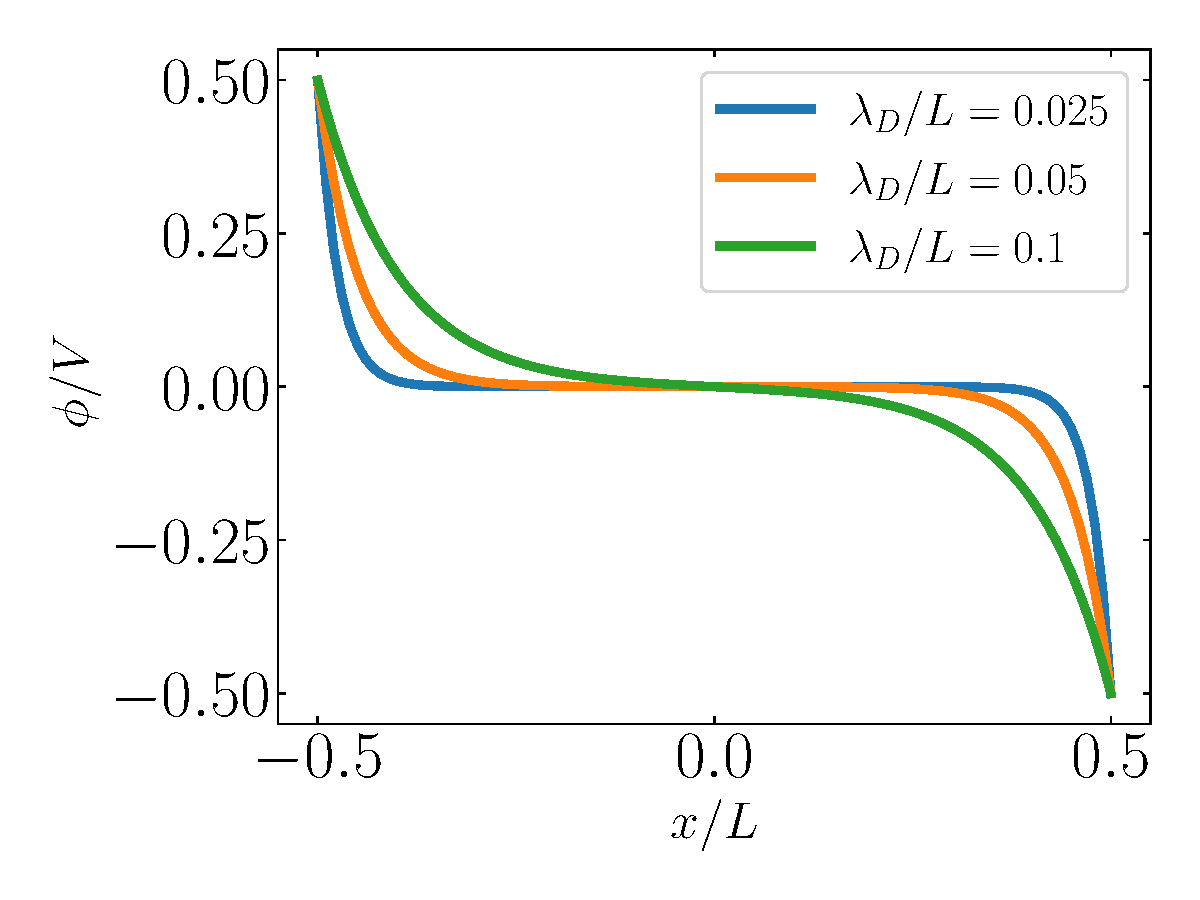
\includegraphics[width=\textwidth]{../images/debye_phi.pdf}
        \caption{}
        \label{fig:debye_phi}
    \end{subfigure}
    \begin{subfigure}[b]{0.45\textwidth}
        \centering
        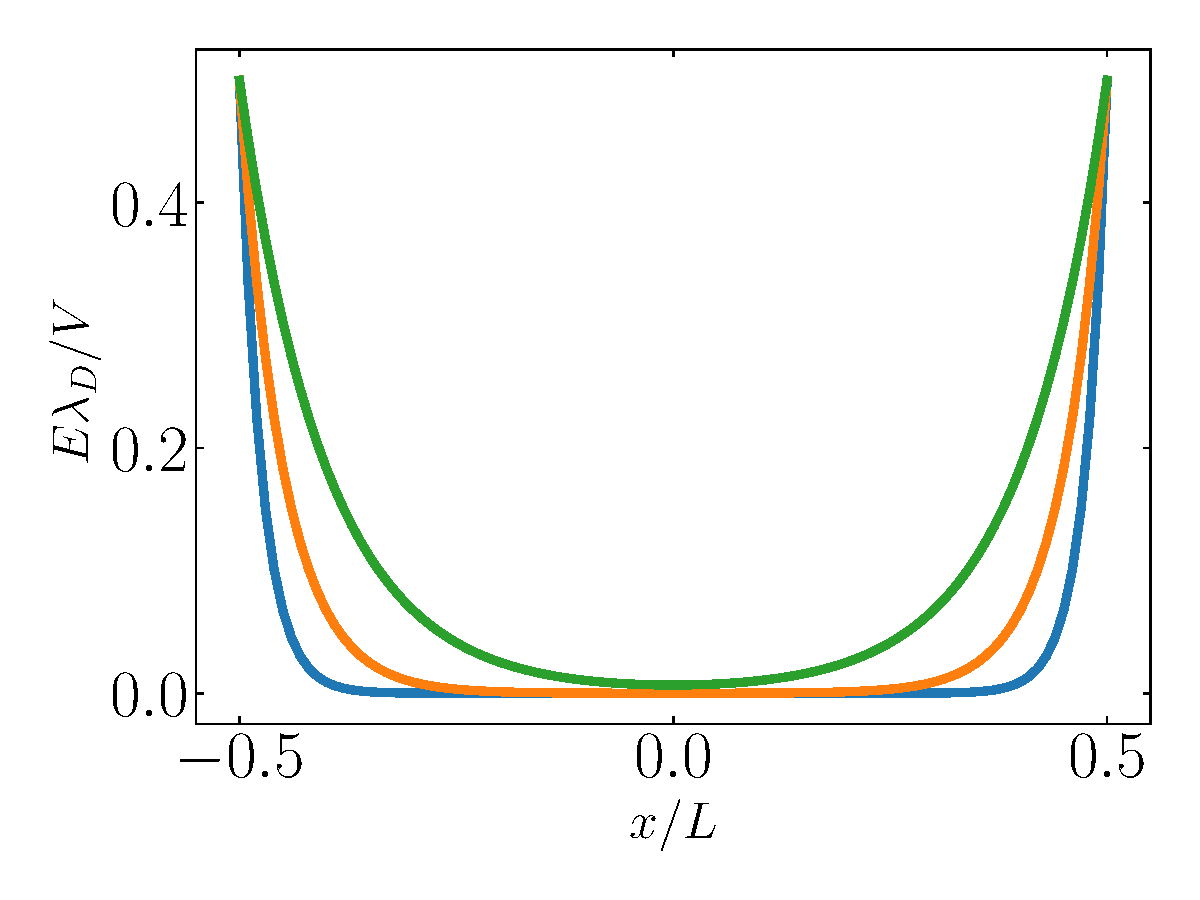
\includegraphics[width=\textwidth]{../images/debye_elec.pdf}
        \caption{}
        \label{fig:debye_elec}
    \end{subfigure}
    \caption{Electric potential and field for various values of $\lambda_D/L$.}
    \label{fig:debye_phi_elec}
\end{figure}

We note that $\lambda_{De}$,  $w_{pe}$, and $v_{Te}$ are all related to each other as shown below
\begin{equation}
    \label{eq:debye_3vars}
    \lambda_{De} w_{pe} = \left ( \frac{\epsilon_0 k_B T_e}{n_{e0} e^2} \right )^{1/2} \left ( \frac{n_{e0} e^2}{m_e \epsilon_0} \right )^{1/2} = \left ( \frac{k_B T_e}{m_e} \right )^{1/2} = v_{Te}.
\end{equation}

%--------------------------------------------
\subsection{Plasma frequency}
%--------------------------------------------
At the end of \cref{sec:ep_waves} we assumed $w_{pe} < w$ in \cref{eq:ep_waves_pre_dispersion} to obtain a dispersion relation for electron-plasma waves. We now consider the cases $w_{pe} > w$ and $w_{pe} = w$ to better understand the role played by the plasma frequency $w_{pe}$.

We first consider the case of $w_{pe} > w$. Plugging in \cref{eq:ep_waves_efield_divergence} in \cref{eq:ep_waves_pre_dispersion} and using the definition of the electric potential, we have 
\begin{equation}
    \label{eq:plasma_freq_quartic}
    (w^2 - w_{pe}^2) \nabla^2 \phi_1 + \gamma_e v_{Te}^2 \nabla^4 \phi_1 = 0.
\end{equation}
We'll use the same setting as that for the derivation of the Debye length. The only difference is that the potential drop across the domain now oscillates with a frequency of $w$, that is $\phi_1(-L/2) - \phi_1(L/2) = V \exp (-iwt)$. Simplifying due to the one-dimensional domain and re-arranging, \cref{eq:plasma_freq_quartic} becomes
\begin{equation*}
     \frac{d^4 \phi_1}{dx^4} - \frac{w_{pe}^2 - w^2}{\gamma_e v_{Te}^2} \frac{d^2 \phi_1}{dx^2} = 0.
\end{equation*}
Using \cref{eq:debye_3vars} the above becomes
\begin{equation*}
    \frac{d^4 \phi_1}{dx^4} - \frac{1}{\gamma_e \lambda_{De}^2} \left ( 1 - \frac{w^2}{w_{pe}^2} \right ) \frac{d^2 \phi_1}{dx^2} = 0,
\end{equation*}
which we re-write as
\begin{equation*}
    \frac{d^4 \phi_1}{dx^4} - \frac{1}{\hat{\lambda}^2_{De}} \frac{d^2 \phi_1}{dx^2} = 0,
\end{equation*}
where 
\begin{equation*}
    \hat{\lambda}_{De}^2 = \gamma_e \lambda_{De}^2 \left ( 1 - \frac{w^2}{w_{pe}^2} \right )^{-1}.
\end{equation*}  
Integrating the fourth-order PDE above twice, we get
\begin{equation*}
    \frac{d^2 \phi_1}{dx^2} - \frac{1}{\hat{\lambda}^2_{De}} \phi_1 + C_1 x + C_2= 0
\end{equation*}
Since to obtain \cref{eq:ep_waves_pre_dispersion} we assumed $n_{e1} = \tilde{n}_{e1} \exp(-iwt)$, where $\tilde{n}_{e1} = \tilde{n}_{e1}(\xvec)$, we'll also assume $\phi_1 = \tilde{\phi}_1 \exp(-iwt)$, where $\tilde{\phi}_1 = \tilde{\phi}_1(\xvec)$. Plugging this into the ODE above we get
\begin{equation*}
     \left (\frac{d^2 \tilde{\phi}_1}{dx^2} - \frac{1}{\hat{\lambda}^2_{De}} \tilde{\phi}_1 \right ) + \left ( \frac{C_1 x + C_2}{\exp(-iwt)} \right )= 0
\end{equation*}
Note that the first term in parenthesis above does not depend on time, and thus the second term in parenthesis should not do so either. This can only be accomplished if we set $C_1 = C_2 = 0$. Thus we finally have
\begin{equation}
    \frac{d^2 \tilde{\phi}_1}{dx^2} - \frac{1}{\hat{\lambda}^2_{De}} \tilde{\phi}_1 = 0.
\end{equation}
The solution to the above that also conforms to the boundary conditions is ...

It is often important to know the plasma density at which the electron plasma frequency $w_{pe}$ equals the external frequency $w$. This density is referred to as the critical density $n_{cr}$. Equating the electron plasma frequency with the external frequency we get
\begin{equation*}
    \frac{n_{cr} e^2}{m_e \epsilon_0} = w^2,
\end{equation*}
which leads to
\begin{equation}
    \label{eq:plas_freq_crit_den}
    n_{cr} = \frac{m_e \epsilon_0 w^2}{e^2}
\end{equation}
The above can be re-written as
\begin{equation*}
    n_{cr} = \frac{m_e \epsilon_0 (2 \pi \nu)^2}{e^2} = \frac{4 \pi^2 m_e \epsilon_0 c^2}{e^2} \frac{1}{\lambda^2} = 1.115 \times 10^{27} \frac{1}{\lambda_{\mu m}^2},
\end{equation*}
where $\lambda_{\mu m}$ is in units of microns and $n_{cr}$ in units of \#/m\textsuperscript{3}.

%--------------------------------------------
\subsection{The coupling parameter}
%--------------------------------------------

Coulomb interactions are those which occur when two charge particles head towards each other. We can define two types of Coulomb interactions: strong and weak. Strong Coulomb interactions are those for which the particle's Coulomb potential energy is larger than its kinetic energy, and viceversa for weak Coulomb interactions. Thus, we can also define two types of plasma regimes:
\begin{itemize}
    \item Strongly-coupled plasmas: plasmas where the Coulomb interactions are mostly strong and thus drive the dynamics of its evolution. Coulomb interactions tend to be strong when the inter-particle distances are small, and thus this regime would be dominated by \textit{short-range} interactions. These plasmas are also described as exhibiting \textit{collisional} behavior, since a strong Coulomb interaction essentially means a collision has occurred.
    \item Weakly-coupled plasmas: plasmas where the Coulomb interactions are mostly weak, and as a result do not drive the dynamics of its evolution. The plasma dynamics are instead driven by \textit{long-range} effects caused by smooth electromagnetic fields that result from integrating a large number of particles. These plasmas are also described as exhibiting \textit{collective} behavior, since the long-range electromagnetic fields follow from the collective integration of many particles.
\end{itemize}

We describe an approximate Coulomb potential energy for particles in a plasma as
\begin{equation}
    U =  \frac{q_\alpha^2}{4 \pi \epsilon_0 a_\alpha}.
\end{equation}
The impact parameter that has been used above is $a_\alpha$, the sphere radius. This provides a decent measure on the average spacing between particles in a plasma. Since the volume of a single particle is $1/n_\alpha$, and if we assume that this volume is given by $4/3 \pi a_\alpha^3$, then equating these two gives the expression for the sphere radius
\begin{equation}
    a_\alpha = \left ( \frac{3}{4 \pi n_\alpha} \right )^{1/3}.
\end{equation}
The thermal velocity of a particle is given by
\begin{equation}
    v_{T_\alpha} = \sqrt{\frac{k_B T_\alpha}{m_\alpha}}
\end{equation}
A measure of the kinetic energy of a particle is given in terms of the thermal velocity as shown below
\begin{equation}
    K = m_\alpha v_{T_\alpha}^2 = k_B T_\alpha
\end{equation}
The ratio of the particle's Coulomb potential energy and its kinetic energy is referred to as the coupling parameter $\Gamma_\alpha$. That is 
\begin{equation}
    \Gamma_\alpha = \frac{q_\alpha^2}{4 \pi \epsilon_0 a_\alpha k_B T_\alpha}.
\end{equation}
$\Gamma_\alpha > 1$ denotes a strongly coupled plasma, and $\Gamma_\alpha < 1$ denotes a weakly coupled plasma. 

%--------------------------------------------
\subsection{The plasma parameter}
%--------------------------------------------
The standard plasma parameter $\Lambda_\alpha$ is defined as
\begin{equation}
    \Lambda_\alpha = \frac{4}{3} \pi \lambda_{D\alpha}^3 n_\alpha.
\end{equation}

There is a one to one relationship between the coupling parameter and the standard plasma parameter. Simple algebra shows that 
\begin{equation}
    \Gamma_\alpha = (1/3) \Lambda_\alpha^{-2/3}.
\end{equation}
Thus, the coupling and plasma parameters are inversely proportional to each other. $\Lambda_\alpha < 1$ implies strongly-coupled plasmas, and $\Lambda_\alpha > 1$ weakly-coupled plasmas. Since $\Lambda_\alpha$ represents the number of particles per Debye sphere, it is interesting to see that a large number of particles within such a sphere is needed to be in the weakly-coupled-plasma regime. However, this does not correspond to a plasma with large density, in fact, it corresponds to the opposite. The explicit $n_\alpha$ term in the definition $\Lambda_\alpha = (4/3) \pi \lambda^3_{D\alpha} n_\alpha$ is dominated by the $n_\alpha$ in the denominator of $\lambda_{D\alpha}$. In other words, low plasma densities lead to large Debye spheres, which in turn leads to many particles per Debye sphere, and hence a weakly-coupled plasma.

%--------------------------------------------
\subsection{Electron degeneracy}
%--------------------------------------------

\begin{itemize}
    \item DeBroglie wavelength
    \begin{equation}
        \lambda_{B\alpha} = \dfrac{h}{\sqrt{2 \pi} m_\alpha v_{T\alpha}}
    \end{equation}
    \item Quantum plasma parameter
    \begin{equation}
        \chi_\alpha = \frac{4}{3} \pi \lambda_{B\alpha}^3 n_\alpha
    \end{equation}
    
    \item Fermi energy:
    \begin{equation}
        E_{f\alpha} = \frac{\hbar^2}{2m_\alpha} \left ( 3 \pi^2 n_\alpha \right)^{2/3}
    \end{equation}

    \item The Fermi energy can be used to define the Fermi temperature $T_{f\alpha}$, Fermi velocity $v_{f\alpha}$, Fermi momentum $p_{f\alpha}$, and Fermi wavevector $k_{f\alpha}$
    \begin{equation}
        E_{f\alpha} = k_B T_{f\alpha} = \frac{1}{2} m_\alpha v_{f\alpha}^2  = \frac{p_{f\alpha}^2}{2m_\alpha} = \frac{\left ( \hbar k_{f\alpha} \right ) ^2}{2m_\alpha}
    \end{equation}

    \item Degeneracy parameter:
    \begin{equation}
        \Theta_\alpha = \frac{k_B T_\alpha}{E_{f\alpha}} = \left( \frac{2^{10} \pi}{3^4} \right)^{1/3} \chi_\alpha^{-2/3}
    \end{equation}
\end{itemize}

%########################################################################
\chapter{Collisions}
%########################################################################
%------------------------------------------------------------------------
\section{Cross section}
%------------------------------------------------------------------------
%--------------------------------------------
\subsection{General definition}
%--------------------------------------------
Two particles traveling towards each other can undergo an interaction. Types of interactions include Coulomb collisions between two charged particles, fusion reactions between ions, and photon-matter phenomena such as Compton scattering, the photoelectric effect, and pair production.

\begin{figure}[ht]
    \centering
    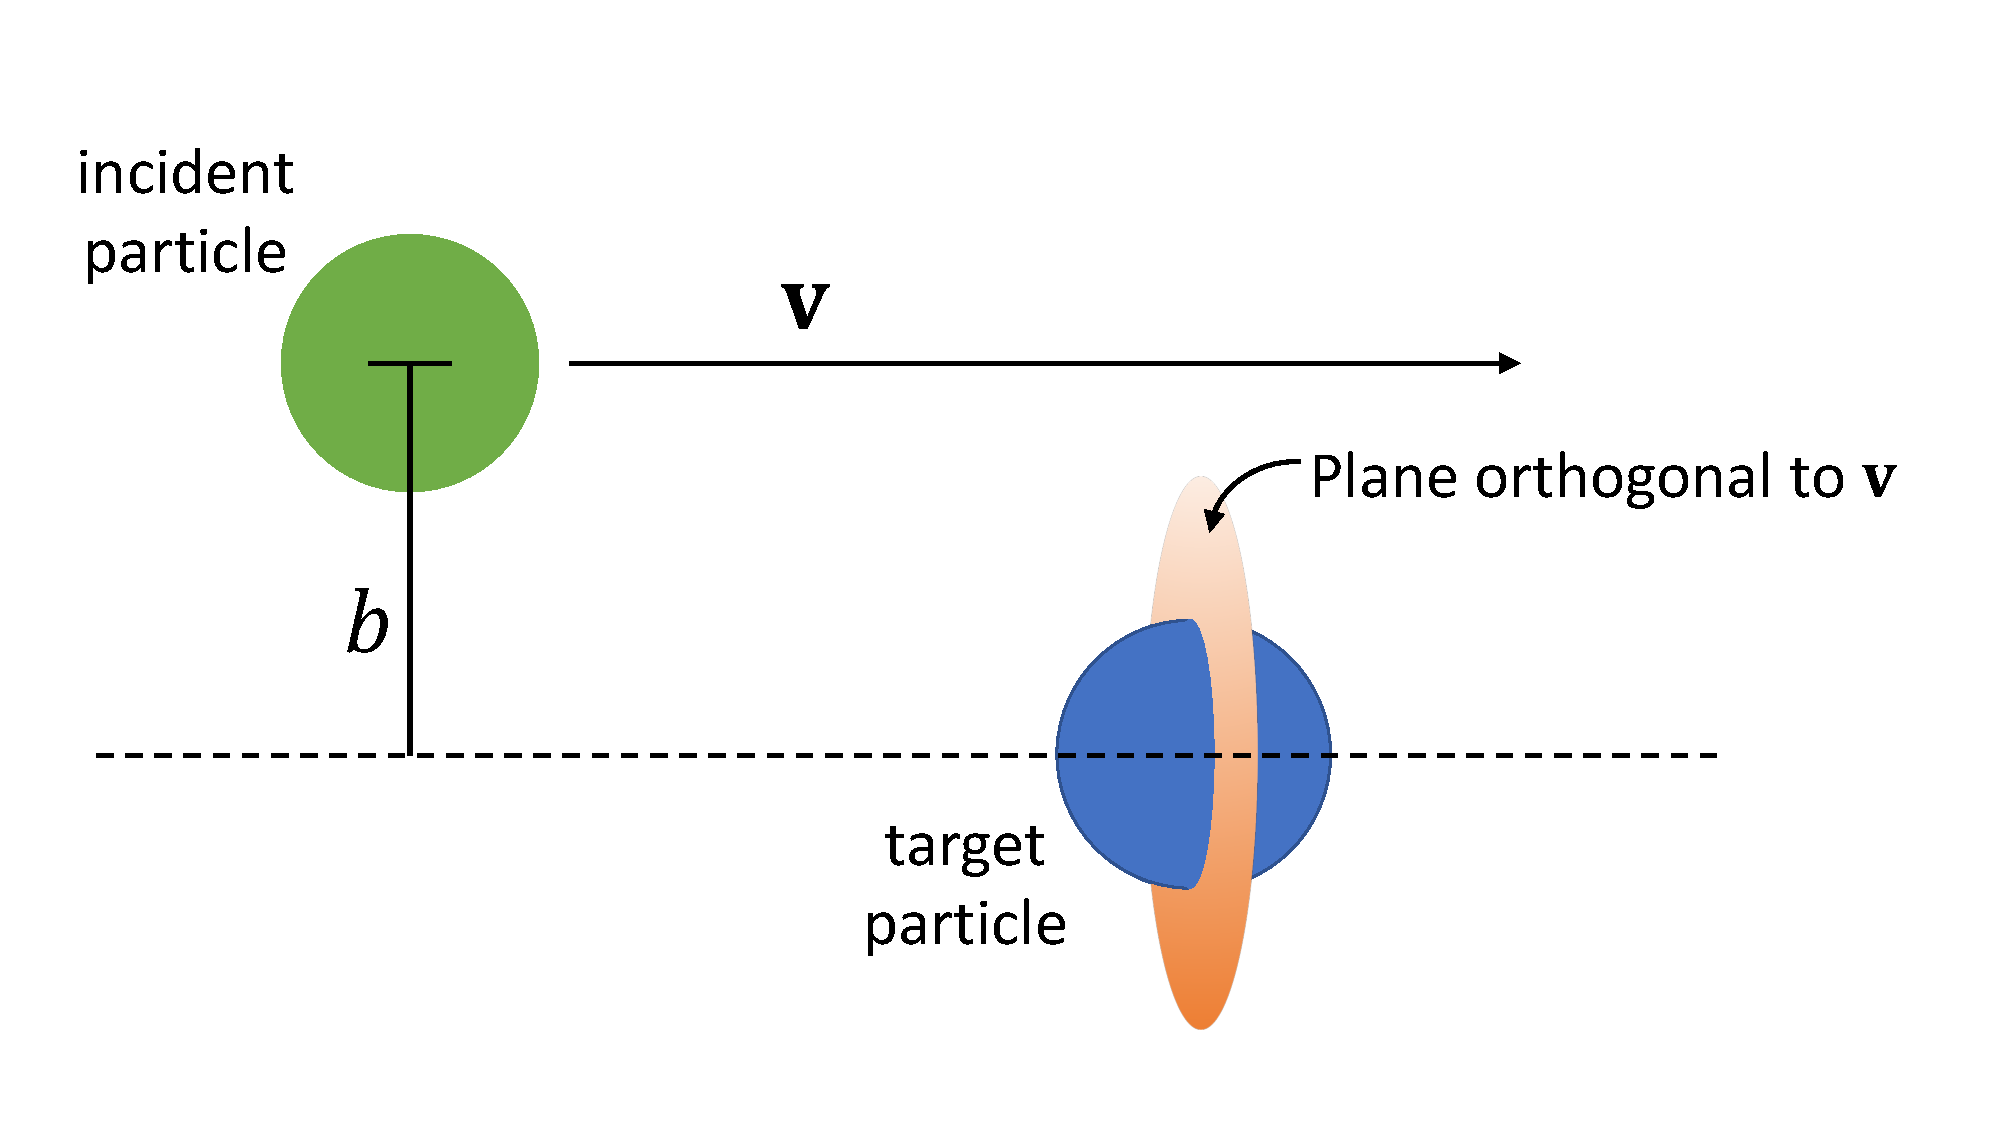
\includegraphics[width=10cm]{../images/cross_section.pdf}
    \caption{Interaction of incident and target particles.}
    \label{fig:cross_many_particles}
\end{figure}
To define the cross section, we'll consider $I$ incident particles heading towards $J$ stationary target particles (see \cref{fig:cross_many_particles}). Not all of the incident particles will interact with the target particles, some will instead continue to travel in a uniform trajectory. The number of incident particles that do interact with the target particles is labeled as $N$. The cross section $\sigma$ is then a constant of proportionality defined by the following equation
\begin{equation}
    \label{eq:cross_def}
    N = \sigma I n_A.
\end{equation}
In the above, $n_A$ is the areal number density, that is, $n_A = J / A = n \Delta x$, where $n$ is the volume number density.

%--------------------------------------------
\subsection{Differential cross section}
%--------------------------------------------
\begin{figure}[ht]
    \centering
    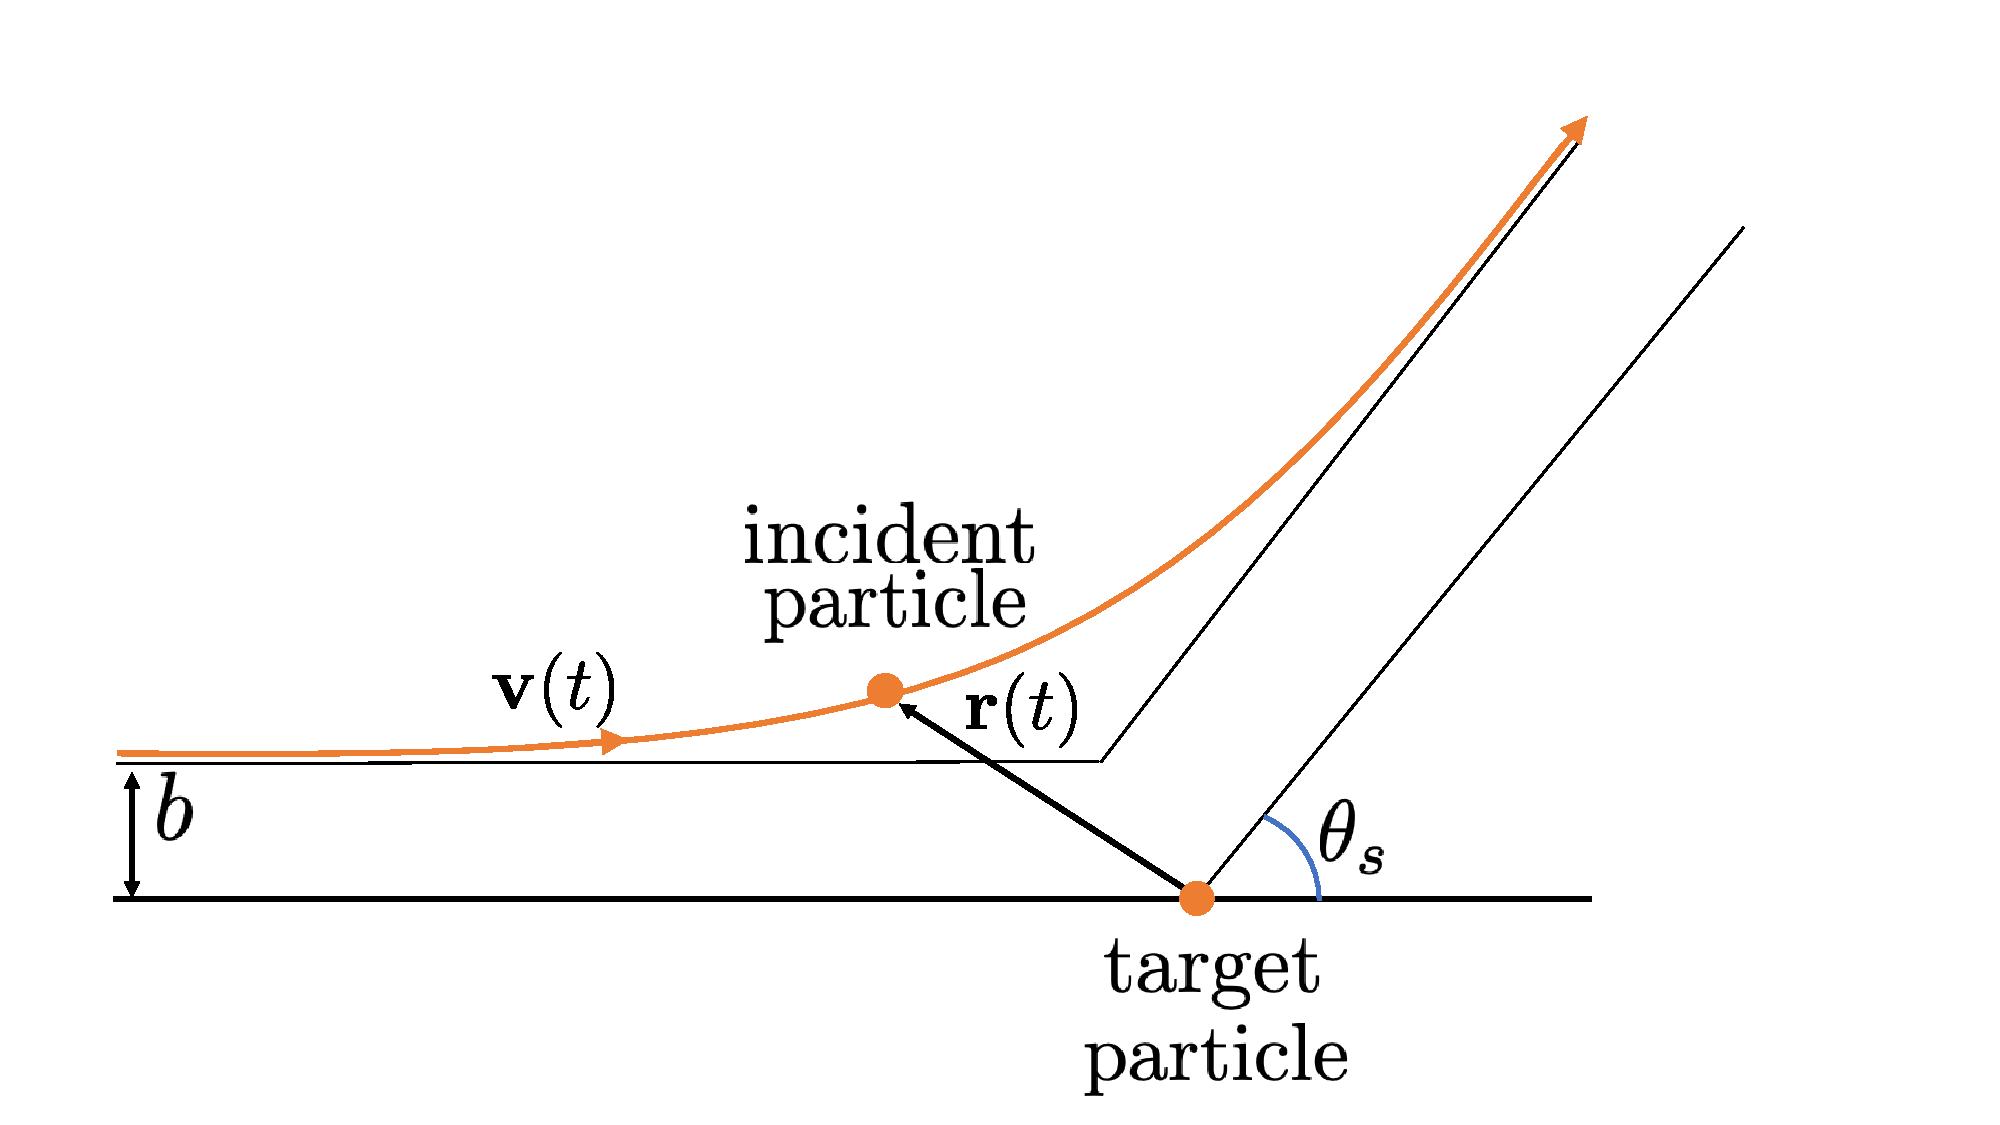
\includegraphics[width=10cm]{../images/scattering.pdf}
    \caption{Depiction of particle scattering.}
    \label{fig:scattering}
\end{figure}

Consider the scattering of two particles: an incident and a target particle. If we fix the reference frame to follow the target particle, then the scattering can be depicted as shown in \cref{fig:scattering}. The displacement parameter is labelled as $b$, and the scattering angle as $\theta_s$. For three dimensional scattering, the encounter is as shown in \cref{fig:scattering_3d}. Not that in that figure the incident particle starts within the $x-z$ plane, and after scattering the particle is confined to a plane that is tilted an angle $\phi_s$ from the $x-z$ plane.

\begin{figure}[ht]
    \centering
    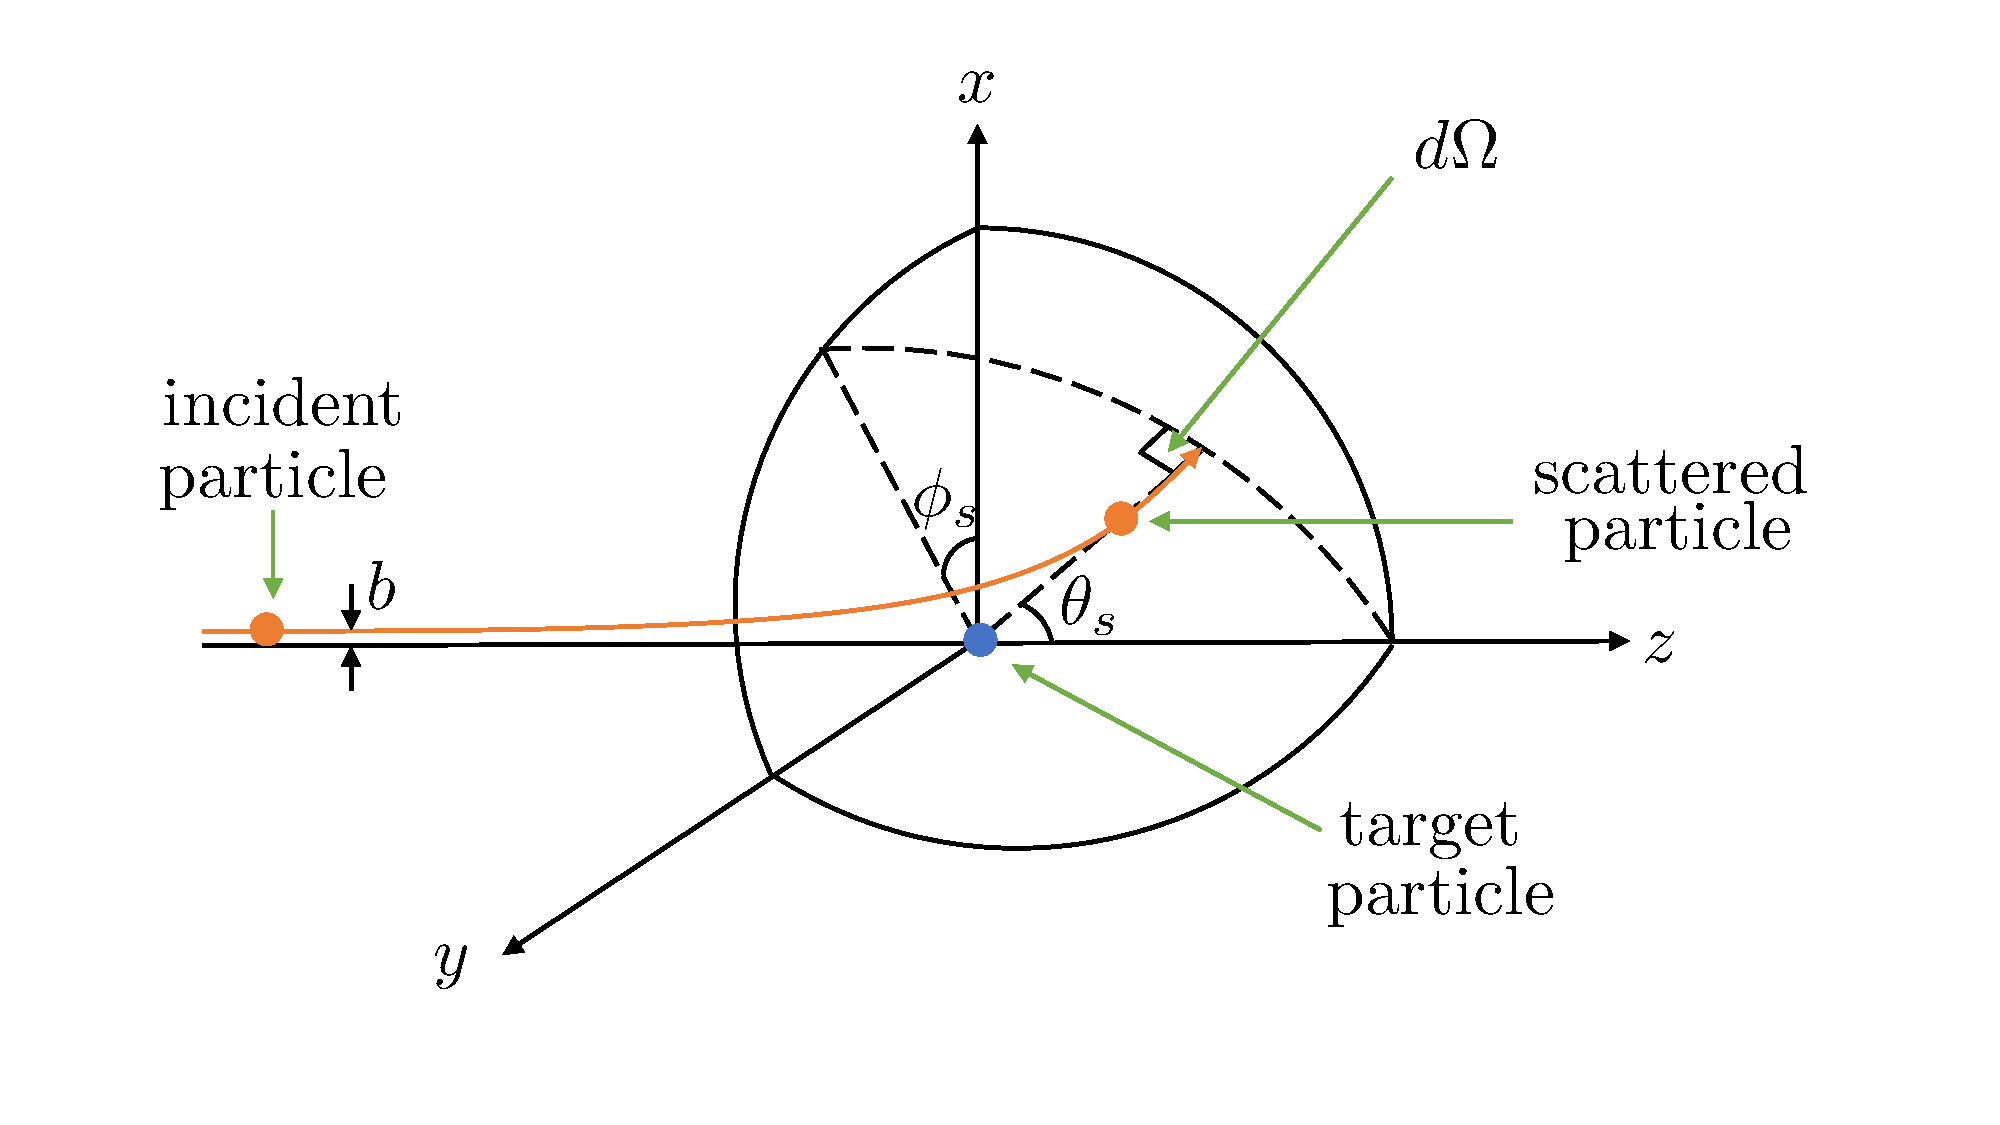
\includegraphics[width=10cm]{../images/scattering_3d.pdf}
    \caption{Depiction of particle scattering in 3D.}
    \label{fig:scattering_3d}
\end{figure}

From the entire set of incident particles $N$ that interact with the target particles, one can define an infinitesimal subset $N_{\theta,\phi} d\Omega$ as the number of particles scattered into an infinitesimal solid angle $d\Omega = \sin \theta_s d\theta_s d\phi_s$, as shown in \cref{fig:scattering_3d}. We note that $N_{\theta,\phi} = N_{\theta,\phi} (\theta_s, \phi_s)$. We introduce the differential cross section
\begin{equation}
    \frac{d\sigma_{\theta,\phi}}{d\Omega} = \frac{d\sigma_{\theta,\phi}}{d\Omega}(\theta_s,\phi_s),
\end{equation}
which is defined by the following expression in an analogous manner to \cref{eq:cross_def},
\begin{equation}
    \label{eq:cross_def_diff}
    N_{\theta, \phi} d\Omega = \left ( \frac{d\sigma_{\theta,\phi}}{d\Omega} d\Omega \right ) I n_A.
\end{equation}
It is best to not think of it as a derivative (what does a derivative with respect to solid angle mean?) and instead to simply think of it as a function that depends on $\theta_s$ and $\phi_s$. Integrating over all $\theta_s$ and $\phi_s$, i.e.
\begin{equation*}
    \int_{\theta_s = 0}^\pi \int_{\phi_s = 0}^{2\pi} N_{\theta, \phi} d\Omega = \int_{\theta_s = 0}^\pi \int_{\phi_s = 0}^{2\pi} \frac{d\sigma_{\theta,\phi}}{d\Omega}  d\Omega I n_A
\end{equation*}
gives \cref{eq:cross_def}.

\begin{figure}[ht]
    \centering
    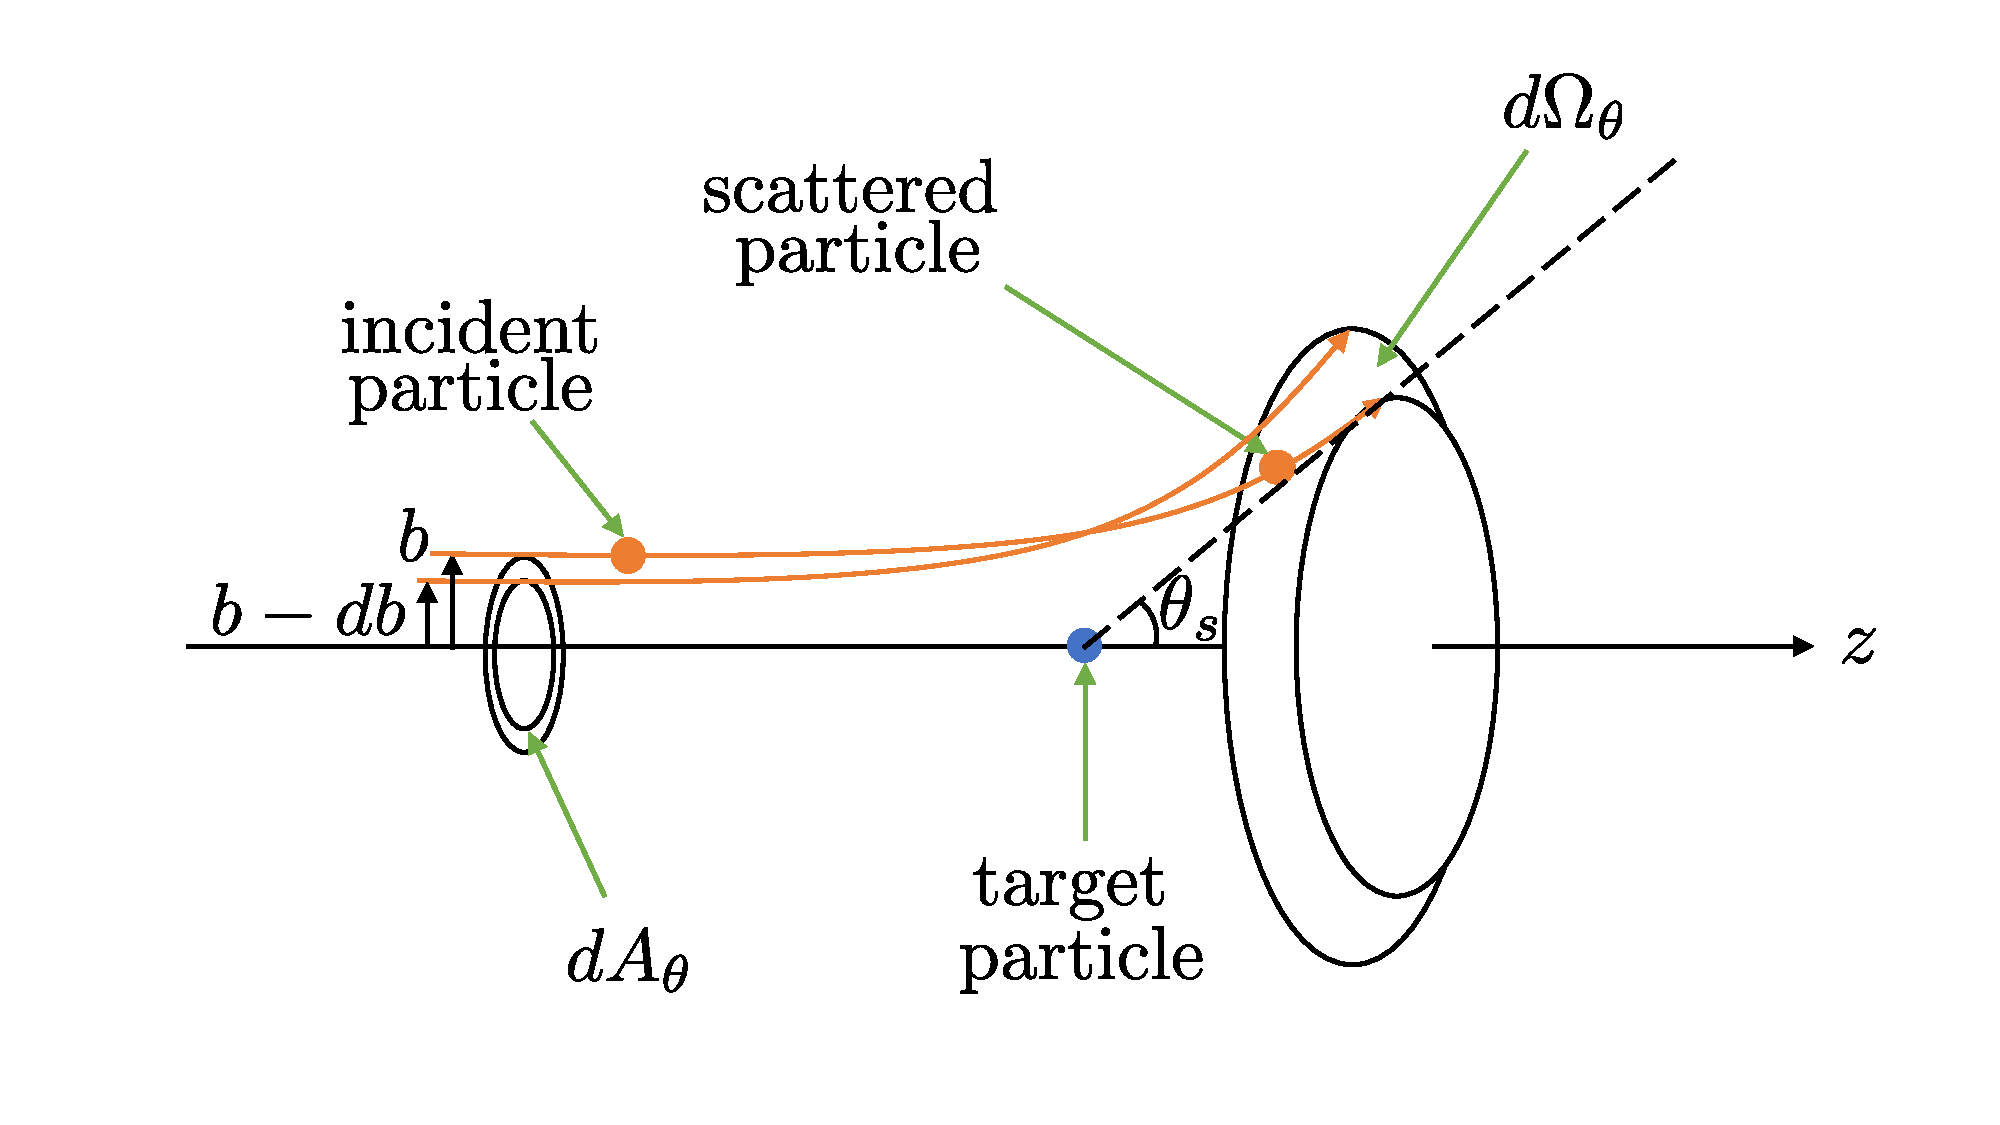
\includegraphics[width=10cm]{../images/scattering_axi.pdf}
    \caption{Depiction of particle scattering in for axisymmetric interactions.}
    \label{fig:scattering_axi}
\end{figure}
For various cases the scattering is axisymmetric, that is, it is independent of $\phi_s$. Thus
\begin{equation*}
    N_{\theta, \phi} \to N_\theta \qquad \frac{d\sigma_{\theta,\phi}}{d\Omega} \to \frac{d\sigma_\theta}{d\Omega},
\end{equation*}
where 
\begin{equation*}
    N_\theta = N_\theta (\theta_s),
\end{equation*}
and
\begin{equation*}
    \frac{d\sigma_\theta}{d\Omega} = \frac{d\sigma_\theta}{d\Omega} (\theta_s).
\end{equation*}
Integrating \cref{eq:cross_def_diff} from $\phi_s = 0$ to $\phi_s = 2\pi$ gives
\begin{equation}
    \label{eq:cross_def_diff_axi}
    N_\theta d\Omega_\theta = \frac{d\sigma_\theta}{d\Omega} d\Omega_\theta I n_A,
\end{equation}
where $d \Omega_\theta = 2\pi \sin \theta_s d\theta_s$. $N_\theta d\Omega_\theta$ thus represents the number of particles that are scattered into the infinitesimal band $d\Omega_\theta$ on a sphere, where $d\Omega_\theta$ is defined by scattering angle $\theta_s$ (see \cref{fig:scattering_axi}). We will note that there is a one-to-one correspondence between the impact parameter $b$ and the scattering angle $\theta_s$, that is, $b = b(\theta_s)$. In other words, any incident particle scattered out through the infinitesimal band $d\Omega_\theta$ would have approached the target-particle through the infinitesimal ring $dA_\theta$ that corresponds to $d\Omega_\theta$. Since there are many target particles, there are many $dA_\theta$'s that correspond to the same $d\Omega_\theta$. Thus, the total number of particles scattered through $d\Omega_\theta$ is given by all the incident particles that cross through the $dA_\theta$'s of all the target particles.

The number of incident particles crossing all the infinitesimal rings $dA_\theta$ is equal to the total number of incident particles $I$ times the probability $P$ that any single incident particle will cross one of those rings. Thus, we can write
\begin{equation*}
    N_\theta d\Omega_\theta = I P.
\end{equation*}
The probability that an incident particle will cross one of those rings is simply the ratio of the surface area covered by all the rings in a section of the target material to the total area of that section. The surface area covered by all the rings in a section of area $S$ is given by $(n_A S) dA_\theta$. Thus, $P = n_A dA_\theta$ and 
\begin{equation*}
    N_\theta d\Omega_\theta = I n_A dA_\theta.
\end{equation*}
We now introduce the differential 
\begin{equation}
    \label{eq:cross_impact_differential}
    db = \frac{db}{d\theta_s} d\theta_s.
\end{equation}
We note that by definition $d\theta_s$ is positive but $db$ can be either positive or negative depending on the sign of $db/d\theta_s$. The infinitesimal area $dA_\theta$ is then given by 
\begin{equation}
    \label{eq:cross_impact_area}
    dA_\theta= 2\pi b |db| = 2 \pi b \left | \frac{db}{d\theta_s} \right | d \theta_s.
\end{equation}
Thus, 
\begin{equation*}
    N_\theta d\Omega_\theta = n_A I 2 \pi b \left | \frac{db}{d\theta_s} \right | d \theta_s.
\end{equation*}
Using \cref{eq:cross_def_diff_axi} in the above, we get
\begin{equation*}
    \frac{d\sigma_\theta}{d\Omega} d\Omega_\theta I n_A = I n_A 2 \pi b \left | \frac{db}{d\theta_s} \right | d \theta_s, 
\end{equation*}
or 
\begin{equation}
    \label{eq:cross_diff_impact_axi}
    \frac{d\sigma_\theta}{d\Omega} = \frac{b}{\sin \theta_s} \left | \frac{db}{d\theta_s} \right |.
\end{equation}

%--------------------------------------------
\subsection{Mean free path \& collision frequency}
%--------------------------------------------
The mean free path can be expressed in terms of the cross section as
\begin{equation}
    \lambda_m = \frac{1}{n_1 \sigma}.
\end{equation}
Given the particle's speed $v$, on can also define the collision time as follows
\begin{equation}
    \tau_m = \frac{\lambda_m}{v} = \frac{1}{n_1 \sigma v}.
\end{equation}
Finally, the collision frequency is simply the inverse of the collision time, that is
\begin{equation}
    \nu_{m} = \frac{1}{\tau_m} = n_1 \sigma v.
\end{equation}

%------------------------------------------------------------------------
\section{Coulomb collisions}
%------------------------------------------------------------------------

%--------------------------------------------
\subsection{Particle equations}
%--------------------------------------------
\label{sec:coulomb_particle_equations}
Consider two particles, with positions $\rvec_1=\rvec_1(t)$ and $\rvec_2=\rvec_2(t)$, velocities $\vvec_1=\vvec_1(t)$ and $\vvec_2=\vvec_2(t)$, charges $q_1$ and $q_2$, and masses $m_1$ and $m_2$, respectively. Their positions and velocities are governed by the following equations 
\begin{equation}
    \label{eq:coul_particle_1_pos}
    \frac{d \rvec_1}{dt} = \vvec_1,
\end{equation}
\begin{equation}
    \label{eq:coul_particle_2_pos}
    \frac{d \rvec_2}{dt} = \vvec_2,
\end{equation}
\begin{equation}
    \label{eq:coul_particle_1_vel}
    m_1 \frac{d\vvec_1}{dt} = -\frac{q_1 q_2}{4 \pi \epsilon} \frac{\rvec_2 - \rvec_1}{\left | \rvec_2 - \rvec_1 \right |^3},
\end{equation}
\begin{equation}
    \label{eq:coul_particle_2_vel}
    m_2 \frac{d\vvec_2}{dt} = -\frac{q_1 q_2}{4 \pi \epsilon} \frac{\rvec_1 - \rvec_2}{\left | \rvec_1 - \rvec_2 \right |^3}.
\end{equation}
We note that the above system consists of twelve equations for twelve unknowns. We now introduce the center-of-mass position $\Rvec = \Rvec(t)$, the center-of-mass velocity $\Vvec = \Vvec(t)$, the shifted position $\rvec = \rvec(t)$ and the shifted velocity $\vvec = \vvec(t)$ as follows
\begin{equation*}
    \Rvec = \frac{m_1 \rvec_1 + m_2 \rvec_2}{m_1 + m_2} \qquad \rvec = \rvec_1 - \rvec_2,
\end{equation*}
\begin{equation*}
    \Vvec = \frac{m_1 \vvec_1 + m_2 \vvec_2}{m_1 + m_2} \qquad \vvec = \vvec_1 - \vvec_2
\end{equation*}
Thus, in terms of these new four variables, the particle equations can be written as
\begin{equation}
    \frac{d \Rvec}{dt} = \Vvec,
\end{equation}
\begin{equation}
    \frac{d \Vvec}{dt} = 0 ,
\end{equation}
\begin{equation}
    \label{eq:particle_pos}
    \frac{d \rvec}{dt} = \vvec,
\end{equation}
\begin{equation}
    \label{eq:coul_particle_vel}
    \frac{d \vvec}{dt} = \frac{q_1 q_2}{4\pi \epsilon_0 m_r} \frac{\rvec}{r^3},
\end{equation}
where the reduced mass $m_r$ is given by
\begin{equation}
    \label{eq:coul_reduced_mass}
    \frac{1}{m_r} = \frac{1}{m_1} + \frac{1}{m_2}.
\end{equation}
The first two equations above give the trivial solution $\Vvec = $ constant and $\Rvec$ = $\Rvec(0) + \Vvec t$. Thus, we have reduced the problem from twelve unknowns to six unknowns, namely $\rvec$ and $\vvec$.

%--------------------------------------------
\subsection{Conservation of energy and momentum}
%--------------------------------------------
Dotting \cref{eq:coul_particle_vel} by $\vvec$ gives 
\begin{align*}
    \vvec \cdot \frac{d \vvec}{dt} &= \frac{q_1 q_2}{4 \pi \epsilon_0 m_r} \vvec \cdot \frac{\rvec}{r^3} \nonumber \\
    &= \frac{q_1 q_2}{4 \pi \epsilon_0 m_r} \frac{d\rvec}{dt} \cdot \frac{\rvec}{r^3} \nonumber \\
    &= \frac{q_1 q_2}{4 \pi \epsilon_0 m_r} \frac{1}{2} \frac{dr^2}{dt} \frac{1}{r^3} \nonumber \\
    &= \frac{q_1 q_2}{4 \pi \epsilon_0 m_r} \frac{1}{r^2} \frac{dr}{dt} \nonumber \\
    &= -\frac{q_1 q_2}{4 \pi \epsilon_0 m_r} \frac{d}{dt} \left ( \frac{1}{r} \right ).
\end{align*} 
For the left hand side above we have
\begin{equation*}
    \vvec \cdot \frac{d \vvec}{dt} = \frac{1}{2} \frac{d v^2}{dt},
\end{equation*}
and thus we obtain the following expression for conservation of energy
\begin{equation*}
    \frac{d}{dt} \left ( \frac{1}{2} m_r v^2 + \frac{q_1 q_2}{4 \pi \epsilon_0} \frac{1}{r} \right ) = 0.
\end{equation*}

Crossing \cref{eq:coul_particle_vel} by $\rvec$ gives
\begin{equation*}
    \rvec \times \frac{d \vvec}{dt} = \frac{q_1 q_2}{4 \pi \epsilon_0 m_r} \frac{\rvec \times \rvec}{r^3} = 0,
\end{equation*}
and thus
\begin{equation*}
    \frac{d}{dt} \left [ m_r \left ( \rvec \times \vvec \right ) \right ] = 0.
\end{equation*}
That is, angular momentum is conserved. A consequence of this is that the vector $\rvec \times \vvec$ is always pointing in the same direction. Thus, if $\rvec(0)$ and $\vvec(0)$ form a plane, then $\rvec(t)$ and $\vvec(t)$ need to reside within that same plane for all times $t$ so that $\rvec(t) \times \vvec(t)$ points in the same direction as $\rvec(0) \times \vvec(0)$. Therefore, the evolution of the position and velocity are confined to a plane and the problem can be reduced from six unknowns to four unknowns. This planar encounter is depicted in \cref{fig:coulomb_scattering}.
\begin{figure}[ht]
    \centering
    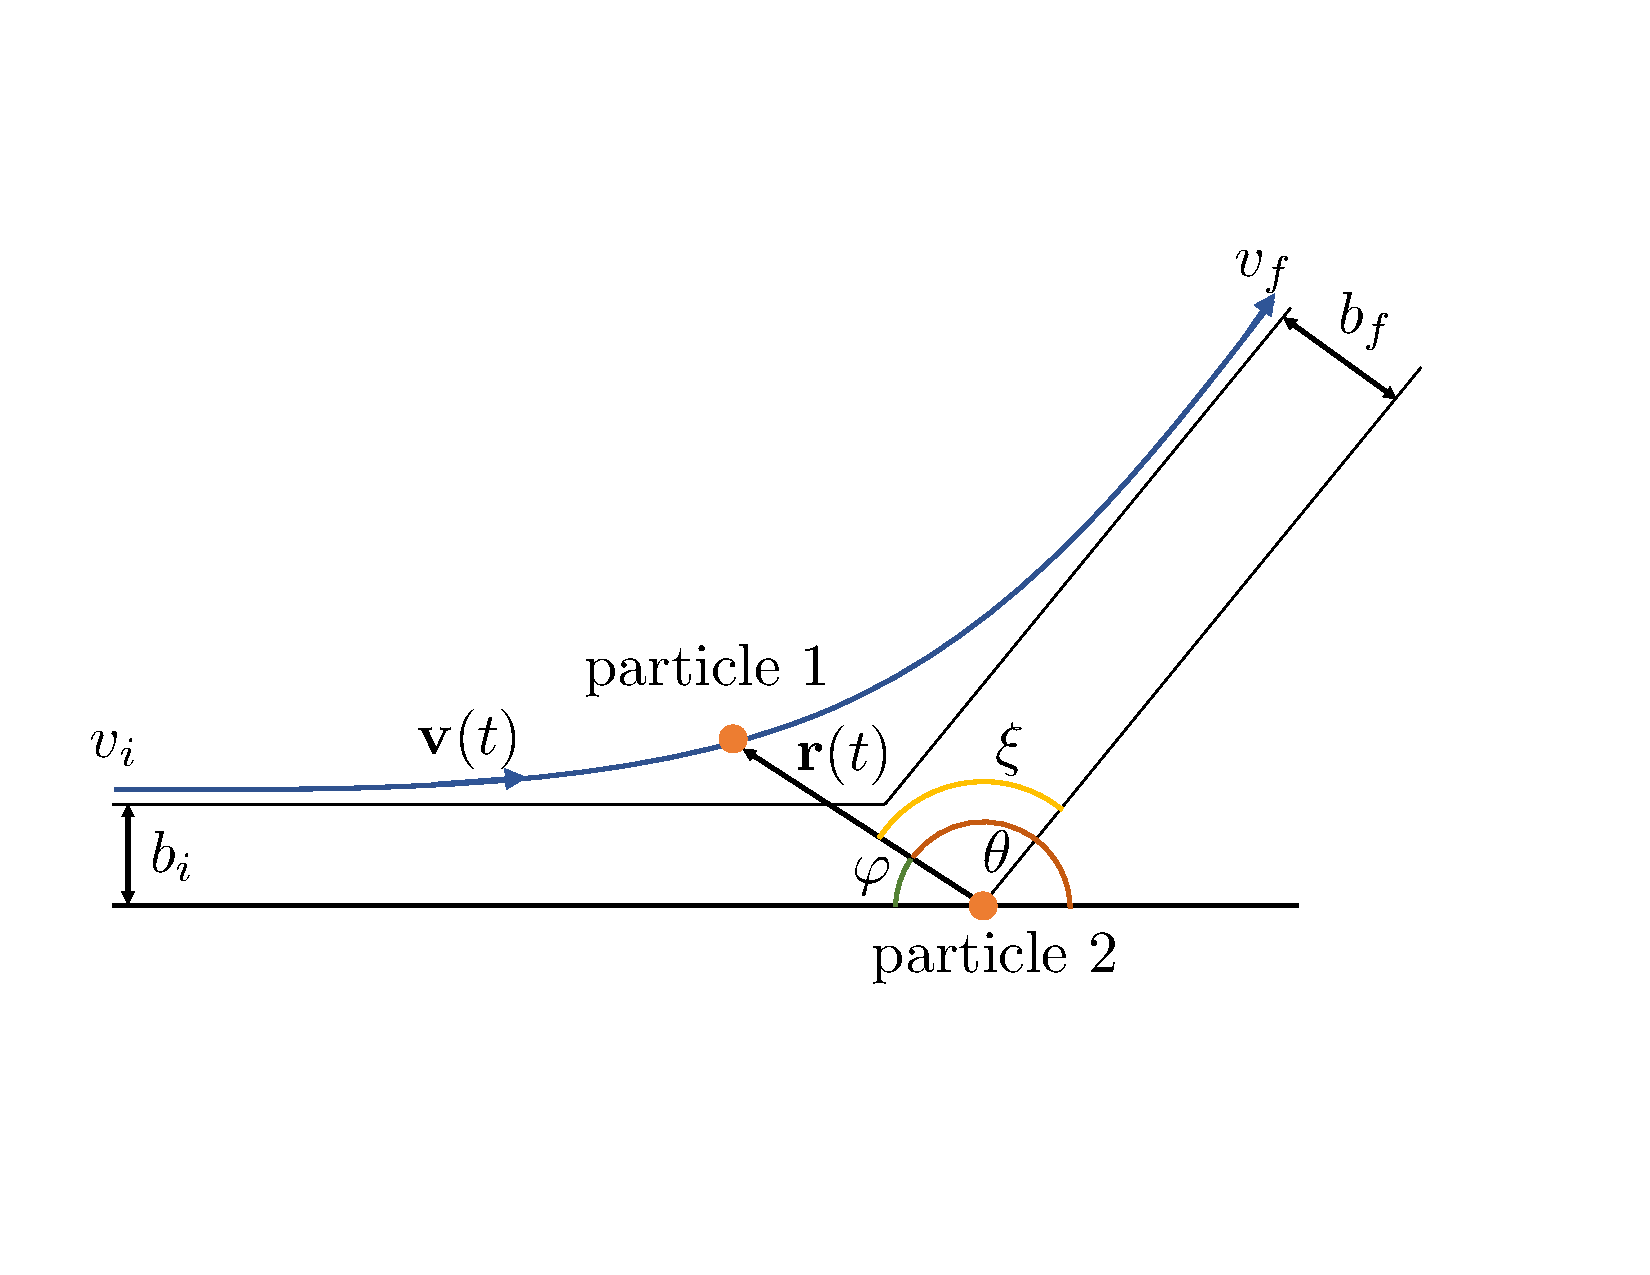
\includegraphics[width=10cm]{../images/coulomb_scattering.pdf}
    \caption{Depiction of Coulomb scattering.}
    \label{fig:coulomb_scattering}
\end{figure}

If we refer to the plane shown in \cref{fig:coulomb_scattering} as the $x-y$ plane, then one can tell that the angular-momentum vector points in the negative $z$ direction. We will denote the magnitude of the conserved angular momentum by $L$, and thus we can write
\begin{equation}
    \label{eq:coul_cons_angular_momentum}
    m_r \left (\rvec \times \vvec \right ) = -L \hat{\zvec}.
\end{equation}

A consequence of both conservation of energy and momentum is as follows. Consider the two limiting states of particle 1---the initial state $v_i$, $b_i$ and the final state $v_f$, $b_f$. Assuming the potential energy is very low at sufficiently early and late times, conservation of energy gives
\begin{equation}
    \frac{1}{2} m_r v_i^2 = \frac{1}{2} m_r v_f^2,
\end{equation}
that is, $v_i=v_f$ (note that for other scattering processes, e.g.\@ Compton scattering, this is not necessarily the case). For the angular momentum of the initial state we have
\begin{multline}
    \label{eq:coul_cons_angular_momentum_derv1}
    m_r \left ( \rvec_i \times \vvec_i \right ) = m_r \sin(-\theta_i) r_i v_i \hat{\zvec} = - m_r \sin(\theta_i) r_i v_i \hat{\zvec} = - m_r \sin(\pi - \varphi_i) r_i v_i \hat{\zvec} \\
    = - m_r \sin(\varphi_i) r_i v_i \hat{\zvec} = -m_r b_i v_i \hat{\zvec}
\end{multline}
Similarly, for the angular momentum of the final state we have
\begin{equation}
    m_r \left ( \rvec_f \times \vvec_f \right ) = m_r \sin(-\xi_f) r_f v_f  \hat{\zvec} = - m_r \sin(\xi_f) r_f v_f \hat{\zvec} = - m_r b_f v_f \hat{\zvec}.
\end{equation}
Equating the last two relationships gives $m_r b_i v_i = m_r b_f v_f$. Since $v_i = v_f$, we finally have $b_i = b_f = b$. Using \cref{eq:coul_cons_angular_momentum} in \cref{eq:coul_cons_angular_momentum_derv1}, we can also write
\begin{equation}
    \label{eq:coul_cons_angular_momentum_mag}
    L = m_r b v_i.
\end{equation}

%--------------------------------------------
\subsection{Polar coordinates}
%--------------------------------------------
\begin{figure}[ht]
    \centering
    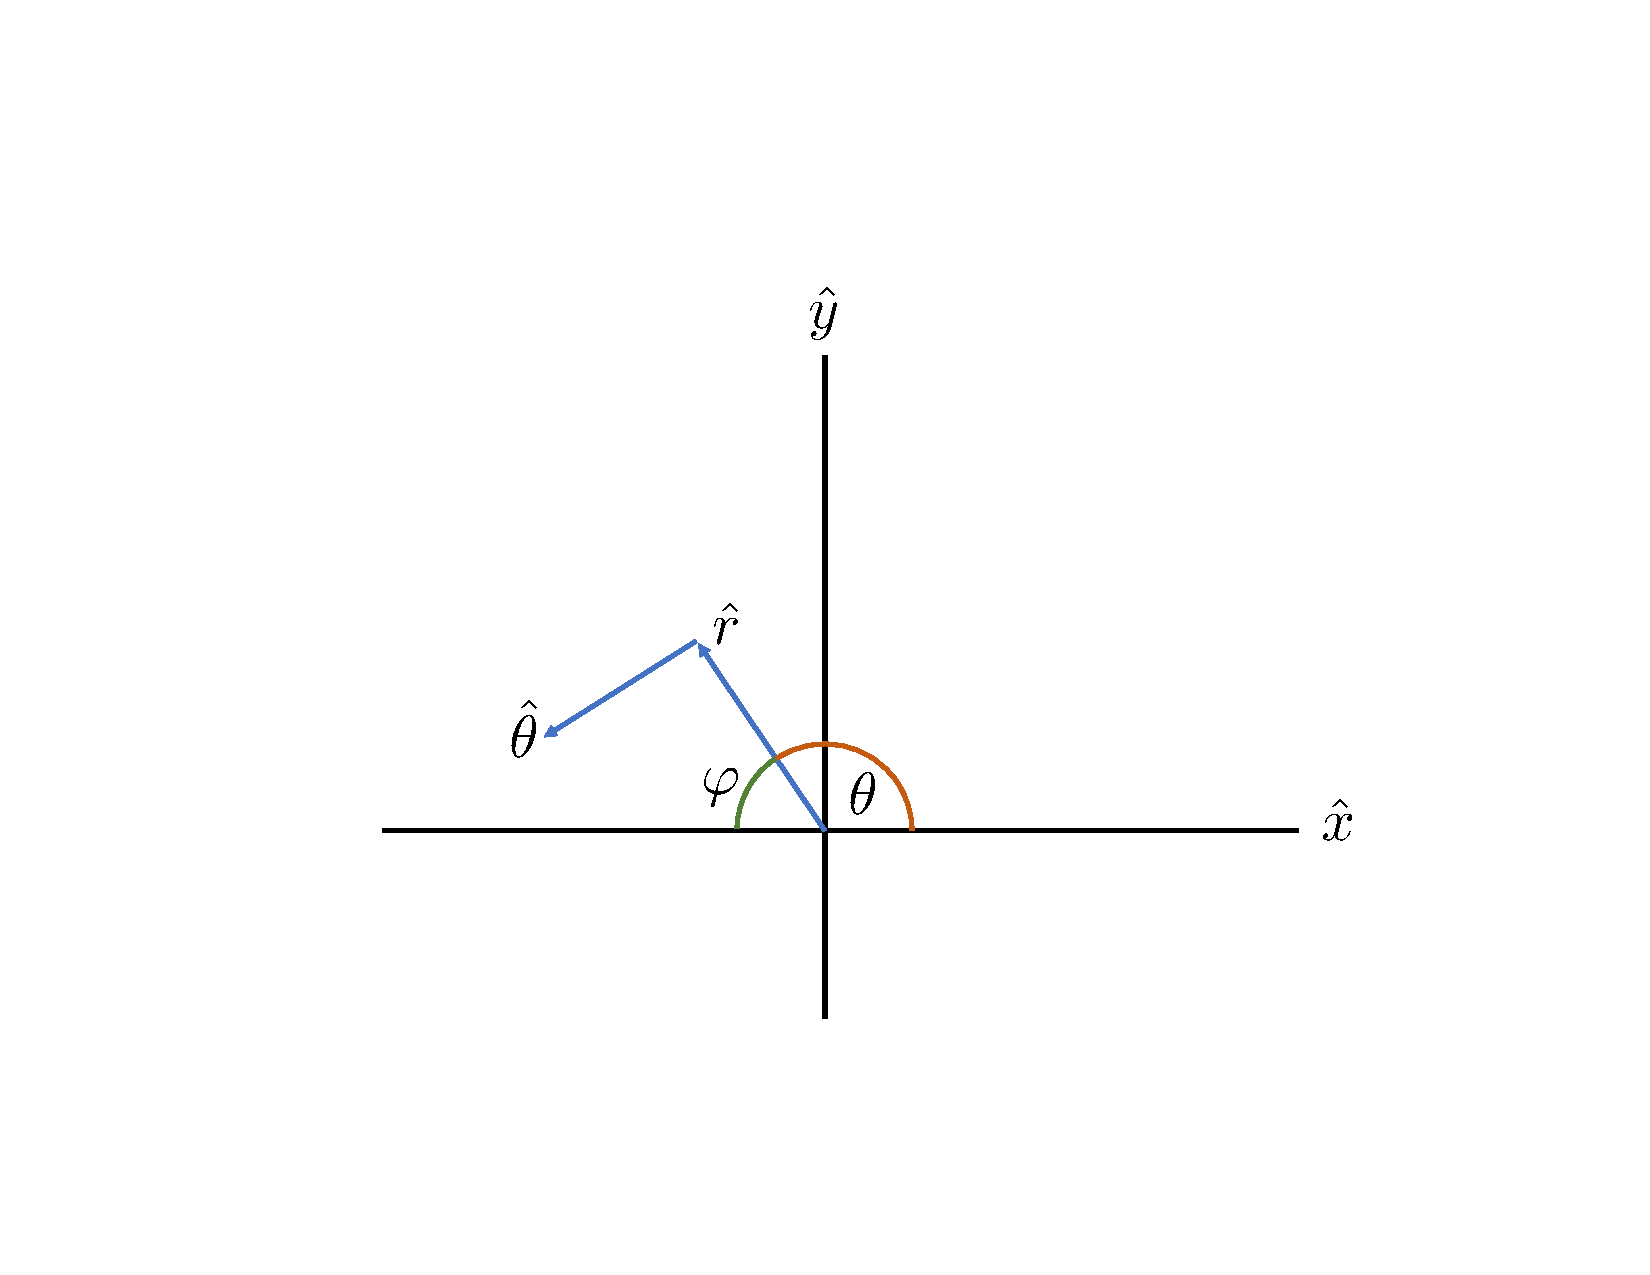
\includegraphics[width=10cm]{../images/polar_coordinates.pdf}
    \caption{Polar coordinates in plane of interaction.}
    \label{fig:polar_coordinates}
\end{figure}

Using polar coordinates, as shown in \cref{fig:polar_coordinates}, we get
\begin{equation*}
    r_x = r \cos \theta = r \cos ( \pi - \varphi ) = -r \cos \varphi,
\end{equation*}
\begin{equation*}
    r_y = r \sin \theta = r \sin ( \pi - \varphi ) = r \sin \varphi.
\end{equation*}

Also, since $\rvec = r \hat{\rvec}$, we have
\begin{align*}
    \vvec = &\frac{d \rvec}{dt} = \frac{dr}{dt} \hat{\rvec} + r \frac{d\hat{\rvec}}{dt} \nonumber \\
    &= \frac{d r}{dt} \hat{\rvec} + r \frac{d\hat{\rvec}}{d\theta} \frac{d\theta}{dt} \nonumber \\
    &= \frac{dr}{dt} \hat{\rvec} + r \frac{d \theta}{dt} \hat{\bm{\theta}},
\end{align*}
and
\begin{align*}
    \frac{d \vvec}{dt} &= \frac{d^2r}{dt^2} \hat{\rvec} + \frac{dr}{dt} \frac{d\hat{\rvec}}{dt} + \frac{d}{dt} \left ( r \frac{d\theta}{dt} \right ) \hat{\bm{\theta}} + r \frac{d \theta}{dt} \frac{d \hat{\bm{\theta}}}{dt} \nonumber \\
    &= \frac{d^2 r}{dt^2} \hat{\rvec} + \frac{dr}{dt} \frac{d\hat{\rvec}}{d\theta} \frac{d\theta}{dt} + \frac{d}{dt} \left ( r \frac{d\theta}{dt} \right ) \hat{\bm{\theta}} + r \frac{d \theta}{dt} \frac{d \hat{\bm{\theta}}}{d\theta} \frac{d \theta}{dt} \nonumber \\
    &= \frac{d^2r}{dt^2} \hat{\rvec} + \frac{dr}{dt} \frac{d\theta}{dt} \hat{\bm{\theta}} + \frac{d}{dt} \left ( r \frac{d\theta}{dt} \right ) \hat{\bm{\theta}} - r \left ( \frac{d\theta}{dt} \right ) ^2 \hat{\rvec}.
\end{align*}

The radial component of \cref{eq:coul_particle_vel} thus becomes 
\begin{equation*}
    \frac{d^2 r}{dt^2} - r \left ( \frac{d\theta}{dt} \right )^2 = \frac{q_1 q_2}{4 \pi \epsilon_0 m_r} \frac{1}{r^2}.
\end{equation*}
Since $\theta = \pi - \varphi$, we have
\begin{equation}
    \label{eq:coul_particle_position_ode}
    \frac{d^2 r}{dt^2} - r \left ( \frac{d\varphi}{dt} \right )^2 = \frac{q_1 q_2}{4 \pi \epsilon_0 m_r} \frac{1}{r^2}.
\end{equation}

For the angular momentum we have
\begin{equation*}
    m_r \rvec \times \vvec = m_r r \hat{\rvec} \times \left ( \frac{dr}{dt} \hat{\rvec} + r \frac{d\theta}{dt} \hat{\bm{\theta}} \right ) = m_r r^2 \frac{d\theta}{dt} \hat{\zvec}
\end{equation*}
Using \cref{eq:coul_cons_angular_momentum}, we can write the above as
\begin{equation}
    \label{eq:coul_particle_cons_angular_polar}
    m_r r^2 \frac{d\varphi}{dt} = L.
\end{equation}

%--------------------------------------------
\subsection{Particle trajectory}
%--------------------------------------------
The goal is to find the radial position of the particle as a function of its angular orientation. That is, we want to find $\tilde{r} = \tilde{r}(\tilde{\varphi})$ such that
\begin{equation}
    \label{eq:coul_particle_position_angle}
    r(t) = \tilde{r}(\varphi(t)).
\end{equation}
To simplify the math, we introduce $\tilde{u} = \tilde{u}(\tilde{\varphi})$ such that $\tilde{u} = 1 / \tilde{r}$. Thus
\begin{equation*}
    \frac{d \tilde{u}}{d\tilde{\varphi}} = -\frac{1}{\tilde{r}^2} \frac{d \tilde{r}}{d\tilde{\varphi}},
\end{equation*}
or, after re-arranging
\begin{equation}
    \label{eq:coul_rgrad_vs_ugrad}
    \frac{d \tilde{r}}{d\tilde{\varphi}} = -\frac{1}{\tilde{u}^2} \frac{d \tilde{u}}{d\tilde{\varphi}}.
\end{equation}

We now proceed as follows. Taking the derivative of $r$, we get
\begin{align}
    \label{eq:coul_particle_derivation_1}
    \frac{dr}{dt} &= \left ( \frac{d \tilde{r}}{d\tilde{\varphi}} \right )_{\tilde{\varphi} = \varphi(t)} \frac{d \varphi}{dt} &&[\cref{eq:coul_particle_position_angle}] \nonumber \\
    &= \left ( -\frac{1}{\tilde{u}^2} \frac{d\tilde{u}}{d\tilde{\varphi}} \right )_{\tilde{\varphi} = \varphi(t)} \frac{d \varphi}{dt} &&[\cref{eq:coul_rgrad_vs_ugrad}]\nonumber \\ 
    &= \left ( -\frac{1}{\tilde{u}^2} \frac{d\tilde{u}}{d\tilde{\varphi}} \right )_{\tilde{\varphi} = \varphi(t)} \frac{L}{m_r r^2} &&[\cref{eq:coul_particle_cons_angular_polar}] \nonumber \\
    &= \left ( -\frac{1}{\tilde{u}^2} \frac{d\tilde{u}}{d\tilde{\varphi}} \frac{L}{m_r \tilde{r}^2} \right )_{\tilde{\varphi} = \varphi(t)} &&[\cref{eq:coul_particle_position_angle}] \nonumber \\
    &= \left ( - \frac{d\tilde{u}}{d\tilde{\varphi}} \frac{L}{m_r} \right )_{\tilde{\varphi} = \varphi(t)}
\end{align}
Taking the derivative of the above, we get
\begin{align}
    \frac{d}{dt} \frac{dr}{dt} &= \left [ \frac{d}{d\tilde{\varphi}} \left ( - \frac{d\tilde{u}}{d\tilde{\varphi}} \frac{L}{m_r} \right ) \right ]_{\tilde{\varphi} = \varphi(t)} \frac{d \varphi}{dt} \nonumber \\
    &= \left ( - \frac{d^2 \tilde{u}}{d\tilde{\varphi}^2} \frac{L}{m_r} \right )_{\tilde{\varphi} = \varphi(t)} \frac{L}{m_r r^2} && [\cref{eq:coul_particle_cons_angular_polar}] \nonumber \\
    &= \left ( - \frac{d^2 \tilde{u}}{d\tilde{\varphi}^2} \frac{L}{m_r} \frac{L}{m_r \tilde{r}^2} \right )_{\tilde{\varphi} = \varphi(t)} && [\cref{eq:coul_particle_position_angle}] \nonumber \\
    &= \left ( - \frac{d^2 \tilde{u}}{d\tilde{\varphi}^2} \frac{L^2 \tilde{u}^2}{m_r^2} \right )_{\tilde{\varphi} = \varphi(t)}
\end{align}
Plugging the last relation into \cref{eq:coul_particle_position_ode} gives
\begin{equation*}
    \left [ - \frac{d^2 \tilde{u}}{d\tilde{\varphi}^2} \frac{L^2 \tilde{u}^2}{m_r^2} - \frac{1}{\tilde{u}} \left ( \frac{L \tilde{u}^2}{m_r} \right )^2 \right ]_{\tilde{\varphi} = \varphi(t)} = \left ( \frac{q_1 q_2}{4 \pi \epsilon_0 m_r} \tilde{u}^2 \right )_{\tilde{\varphi} = \varphi(t)},
\end{equation*}
which, upon re-arranging and dropping the $\varphi(t)$ dependance, becomes
\begin{equation}
    \frac{d^2 \tilde{u}}{d \tilde{\varphi}^2} + \tilde{u} = -\frac{q_1 q_2 m_r}{4 \pi \epsilon_0 L^2}
\end{equation}

Using \cref{eq:coul_cons_angular_momentum_mag} we write the evolution equation for $\tilde{u}$ as
\begin{equation}
    \frac{d^2 \tilde{u}}{d \tilde{\varphi}^2} + \tilde{u} = -\frac{q_1 q_2}{4 \pi \epsilon_0 m_r b^2 v_i^2}.
\end{equation}
Introducing the notation
\begin{equation}
    \label{eq:coul_b90}
    b_{90} = \frac{q_1 q_2}{4 \pi \epsilon_0 m_r v_i^2},
\end{equation}
the evolution equation for $\tilde{u}$ can be simply expressed as
\begin{equation}
    \label{eq:coul_particle_u_equation}
    \frac{d^2 \tilde{u}}{d \tilde{\varphi}^2} + \tilde{u} = -\frac{b_{90}}{b^2}.
\end{equation}

The boundary conditions for \cref{eq:coul_particle_u_equation} are as follows
\begin{equation}
    \label{eq:coul_particle_bc_1}
    \text{as } \varphi(t) \to 0, \quad r(t) \to \infty
\end{equation}
\begin{equation}
    \label{eq:coul_particle_bc_2}
    \text{as } \varphi(t) \to 0, \quad \frac{dr(t)}{dt} \to -v_i
\end{equation}
Given \cref{eq:coul_particle_position_angle}, \cref{eq:coul_particle_bc_1} can only be satisfied if as $\tilde{\varphi} \to 0$, $\tilde{r} \to \infty$. Thus, we also have, as $\tilde{\varphi} \to 0$, $\tilde{u} \to 0$. Similarly, given \cref{eq:coul_particle_derivation_1}, \cref{eq:coul_particle_bc_2} can only be satisfied if as $\tilde{\varphi} \to 0$
\begin{equation*}
    \frac{d\tilde{u}}{d\tilde{\varphi}} \frac{L}{m_r} \to v_i.
\end{equation*}
Using \cref{eq:coul_cons_angular_momentum_mag} we rewrite the above as 
\begin{equation*}
    \frac{d\tilde{u}}{d\tilde{\varphi}} \to \frac{1}{b}.
\end{equation*}

The general solution to \cref{eq:coul_particle_u_equation} is 
\begin{equation*}
    \tilde{u} = A \cos \tilde{\varphi} + B \sin \tilde{\varphi} - \frac{b_{90}}{b^2}.
\end{equation*}
Applying the boundary conditions, we get
\begin{equation*}
    \tilde{u} = \frac{b_{90}}{b^2} \cos \tilde{\varphi} + \frac{1}{b} \sin \tilde{\varphi} - \frac{b_{90}}{b^2},
\end{equation*}
which we finally re-write as
\begin{equation}
    \label{eq:coul_trajectory_eq}
    \frac{1}{\tilde{r}} = \frac{1}{b} \sin \tilde{\varphi} + \frac{b_{90}}{b^2} \left ( \cos \tilde{\varphi} - 1 \right ).
\end{equation}

%--------------------------------------------
\subsection{The scattering angle}
%--------------------------------------------
We now drop the tilde notation for the sake of simplicity. That is, for the radial location of an incident particle, we have
\begin{equation}
    \label{eq:coul_trajectory_eq2}
    \frac{1}{r} = \frac{1}{b} \sin \varphi + \frac{b_{90}}{b^2} \left ( \cos \varphi - 1 \right ),
\end{equation}
where $\varphi$ is the independent variable and $r = r(\varphi)$. We want to know the value of $\varphi$ as $r$ goes to infinity. Using \cref{eq:coul_trajectory_eq2}, and labeling this angle as $\varphi_s$, we have
\begin{equation*}
    0 = \sin \varphi_s + \frac{b_{90}}{b} \left ( \cos \varphi_s - 1 \right ).
\end{equation*}
We express the above in terms of the scattering angle $\theta_s = \pi - \varphi_s$,
\begin{equation*}
    0 = \sin (\pi - \theta_s) + \frac{b_{90}}{b} \left [ \cos \left (\pi - \theta_s \right ) - 1 \right ].
\end{equation*}
or
\begin{equation*}
    0 = \sin \theta_s + \frac{b_{90}}{b} \left ( -\cos \theta_s - 1 \right ).
\end{equation*}
Re-writing the above as
\begin{equation*}
    \frac{\cos \theta_s + 1}{\sin \theta_s} = \frac{b}{b_{90}},
\end{equation*}
and using the trig identity $\cot (\theta/2) = (\cos \theta + 1) / \sin \theta$, we get 
\begin{equation}
    \label{eq:coul_scattering_angle}
    \cot \left ( \frac{ \theta_s }{2} \right ) = \frac{b}{b_{90}}.
\end{equation}

%--------------------------------------------
\subsection{The differential cross section}
%--------------------------------------------

The differential cross section for Coulomb scattering can be computed by making use of \cref{eq:cross_diff_impact_axi}, which is repeated below
\begin{equation}
    \tag{\ref{eq:cross_diff_impact_axi}}
    \frac{d\sigma_\theta}{d\Omega} = \frac{b}{\sin \theta_s} \left | \frac{db}{d\theta_s} \right |.
\end{equation}
From \cref{eq:coul_scattering_angle} we get,
\begin{equation}
    \frac{db}{d\theta} = -\frac{b_{90}}{2} \frac{1}{\sin^2 (\theta_s / 2)},
\end{equation}
which, plugging in \cref{eq:cross_diff_impact_axi}, gives
\begin{equation*}
    \frac{d\sigma_\theta}{d\Omega} = \left [ b_{90}\frac{\cot(\theta_s/2)}{\sin \theta_s} \right ] \left [ \frac{b_{90}}{2} \frac{1}{\sin^2 (\theta_s / 2)} \right ].
\end{equation*}
Using the trig identities $\cot(\theta) = \cos(\theta) / \sin(\theta)$ and $\sin(\theta) = 2 \sin(\theta/2) \cos(\theta/2)$ we get
\begin{equation}
    \frac{d\sigma_\theta}{d\Omega} = \frac{b_{90}^2}{4} \frac{1}{\sin^4 (\theta_s/2)}.
\end{equation}

%--------------------------------------------
\subsection{Collision integral}
%--------------------------------------------
\begin{equation}
    \Omega_{\alpha \beta}^{(lk)} = \sqrt{ \frac{k_B T}{2 \pi M_{\alpha \beta}} } \int_0^\infty e^{-g^2} g^{2k+3} \phi_{\alpha \beta}^{(l)} \, dg.
\end{equation}
In the above $M_{\alpha \beta}$ is the reduced mass, given by
\begin{equation}
    M_{\alpha \beta} = \frac{M_\alpha M_\beta}{M_\alpha + M_\beta},
\end{equation}
and $\phi^{(l)}_{\alpha \beta}$ is the collision cross section for a given velocity, and is computed as
\begin{equation}
    \phi_{\alpha \beta}^{(l)} = 2 \pi \int_0^\infty \left ( 1 - \cos^l \chi_{\alpha \beta} \right ) b \, db.
\end{equation}
The scattering angle $\chi_{\alpha \beta}$ is given by
\begin{equation}
    \chi_{\alpha \beta} = \pi - 2 \int_{r_{\alpha \beta}^{\text{min}}}^\infty \frac{b}{r^2 \left [ 1 - \frac{b^2}{r^2} - \frac{V_{\alpha \beta (r)}}{g^2 k_B T} \right ]^{1/2} } \, dr.
\end{equation}

For a Coulombic interaction between ions, we can define the natural scale fore the cross-sectional area as
\begin{equation}
    \phi^{(0)}_{\alpha \beta} = \frac{ \pi \left (Z_\alpha Z_\beta e^2 \right)^2}{ \left(2 k_B T\right)^2}.
\end{equation}
Given this definition, we express the collision integral as
\begin{equation}
    \Omega_{\alpha \beta} = \sqrt{ \frac{\pi }{M_{\alpha \beta}}} \frac{( Z_\alpha Z_\beta e^2)^2 }{(2 k_B T )^{3/2}} \mathcal{F}^{lk}_{\alpha \beta},
\end{equation}
where
\begin{equation}
    \mathcal{F}^{(lk)}_{\alpha \beta} = \frac{1}{2 \phi_0} \int_0^\infty e^{-g^2} g^{2k+3} \phi_{\alpha \beta}^{(l)} \, dg
\end{equation}
We note that $\mathcal{F}^{(lk)}_{\alpha \beta} = 4 \mathcal{K}_{lk}(g_{\alpha \beta})$, where $\mathcal{K}_{lk}(g_{\alpha \beta})$ is the notation from the Stanton-Murillo paper.

%%%%%%%%%%%%%%%%%%%%%%%%%%%%%%%%%%%%%%%%%%%%%%%%%%%%%%%%%%%%%%%%%%%%%%%%%
\part{Hydrodynamics}
%%%%%%%%%%%%%%%%%%%%%%%%%%%%%%%%%%%%%%%%%%%%%%%%%%%%%%%%%%%%%%%%%%%%%%%%%

%########################################################################
\chapter{Kinematics of fluid motion}
%########################################################################

%------------------------------------------------------------------------
\section{Eulerian \& Lagrangian reference frames}
%------------------------------------------------------------------------
There are two types of frameworks used to described properties of fluids: Eulerian and Lagrangian. The Eulerian framework is used to describe fields, for which fluid properties are of the form $\fvec = \fvec(t,\xvec)$, where $t$ and $\xvec$ denote time and position. Lagrangian fields are used to describe moving particles, for which fluid properties are of the form $\fvec^+ = \fvec^+(t,\yvec)$, where $t$ denotes time and $\yvec$ the location of the particle at an initial time. Eulerian and Lagrangian properties are related to each other according to 
\begin{equation}
\fvec^+(t,\yvec)=\fvec(t,\xvec^+(t,\yvec)).
\end{equation}

There are two Lagrangian properties that deserve further attention. The position and velocity of a particle are given by $\xvec^+ = \xvec^+(t,\yvec)$ and $\vvec^+ = \vvec^+(t,\yvec)$, respectively. These two are related to each other according to 
\begin{equation}
\frac{\partial \xvec^+}{\partial t} = \vvec^+.
\end{equation}

%------------------------------------------------------------------------
\section{Material derivative}
%------------------------------------------------------------------------

We are interested in knowing how $\fvec^+(t,\yvec)$ for a hypothetical particle changes as we move along the particle's path. Applying the chain rule and product rule,
\begin{align}
\frac{\partial}{\partial t} \fvec^+(t,\yvec)&= \frac{\partial}{\partial t} \fvec(t,\xvec^+(t,\yvec)) \nonumber \\
&=  \frac{\partial}{\partial t} \fvec(t,x_1^+(t,\yvec), x_2^+(t,\yvec), x_3^+(t,\yvec)) \nonumber \\
&=\left( \frac{\partial \fvec(t,x_1,x_2,x_3)}{\partial t}\right )_{\xvec=\xvec^+(t,\yvec)} + \frac{\partial x_1^+(t,\yvec)}{\partial t} \left ( \frac{\partial \fvec(t,x_1,x_2,x_3)}{\partial x_1} \right )_{\xvec = \xvec^+(t,\yvec)} + ...\nonumber \\
&=\left ( \frac{\partial \fvec(t,x_1,x_2,x_3)}{\partial t} \right)_{\xvec=\xvec^+(t,\Yvec)} + v_1^+(t,\yvec) \left ( \frac{\partial \fvec(t,x_1,x_2,x_3)}{\partial x_1} \right )_{\xvec=\xvec^+(t,\yvec),..} + ...
\end{align}
In abridged notation this becomes
\begin{equation}
\label{eq:material_derivative_generic}
\boxed{
\frac{\partial \fvec^+}{\partial t} = \left ( \frac{\partial \fvec}{\partial t} \right)_{\xvec=\xvec^+} + \vvec^+ \cdot ( \nabla \fvec)_{\xvec=\xvec^+}
}
\end{equation}

For an arbitrary particle, the Lagrangian velocity $\vvec^+$ has an Eulerian counterpart $\vvec=\vvec(t,\xvec)$ such that the following is satisfied $\vvec^+ = \vvec(t,\xvec^+)$. For this same particle, we can also introduce the Lagrangian variable $\uvec^+ = \uvec^+(t,\yvec)$ and the Eulerian counterpart $\uvec = \uvec(t,\xvec)$, such that the following is satisfied $\uvec^+ = \uvec(t,\xvec^+)$. We emphasize that $\uvec^+$ is not the velocity of the particle, it is instead an additional particle property since $\vvec^+$ is the actual velocity of the particle. There is a special type of particle, referred to as a fluid particle, which is one that moves with the flow. For this particle $\vvec = \uvec$. We denote properties of a fluid particle with the subscript $u$, e.g. $\xvec^+_u$, $\fvec^+_u$, etc.

Given the the particle property $\fvec^+_u = \fvec(t,\xvec^+_u)$, we have
\begin{align}
\label{eq:kinematic_material_derivative_fluid}
\frac{\partial \fvec^+_u}{\partial t} &=\left(\frac{\partial \fvec}{\partial t}\right)_{\xvec=\xvec^+_u} + \vvec^+_u \cdot \left(\nabla \fvec\right)_{\xvec=\xvec^+_u} \nonumber \\
&=\left(\frac{\partial \fvec}{\partial t} + \uvec \cdot \nabla \fvec\right)_{\xvec=\xvec^+_u}.
\end{align}
The term in parenthesis above is referred to as the material derivative, and it is labeled as
\begin{equation}
\label{eq:material_derivative_definition}
    \frac{D\fvec}{Dt} = \frac{\partial \fvec}{\partial t} + \uvec \cdot \nabla \fvec.
\end{equation}

An application of the above follows. Say we are given a fluid whose temperature and velocity fields are $T$ and $u$, respectively. The PDE for temperature is
\begin{equation}
\label{eq:sample_pde}
\frac{\partial T}{\partial t} + u\frac{\partial T}{\partial x} = \frac{\partial^2 T}{\partial x^2}.
\end{equation}
We now introduce a fluid particle with Lagrangian temperature $T^+_u = T^+_u(t,y)$. This Lagrangian property is related to its corresponding Eulerian field by $T^+_u(t,y) = T_u(t,x^+_u(t,y))$. Using \cref{eq:kinematic_material_derivative_fluid} we find the rate of change of $T^+_u$ to be
\begin{equation}
\frac{\partial T^+_u}{\partial t} = \left( \frac{\partial T}{\partial t} +  u\frac{\partial T}{\partial x} \right)_{x = x^+_u} = \left ( \frac{\partial^2 T}{\partial x^2} \right)_{x = x^+_u}. 
\end{equation}
Thus, we can interpret the PDE as describing the rate of change of a particle's property as the particle moves through space. This rate of change is given by the RHS term of \cref{eq:sample_pde} evaluated at the particle's position. 

%------------------------------------------------------------------------
\section{Reynolds transport theorem}
%------------------------------------------------------------------------
Define the one-dimensional domain $[a_0,b_0]$. Also define the one-dimensional domain $L^+ = L^+(t,a_0,b_0)$, which is given by 
\begin{equation}
    L^+ = \{ x^+ : y \in [a_0,b_0] \}.
\end{equation}
Note that $L^+(0,a_0,b_0) = [a_0,b_0]$. The left boundary of this volume is given by $a^+ = a^+(t,a_0,b_0)$ and the right boundary by $b^+=b^+(t,a_0,b_0)$. These satisfy $a^+(0,a_0,b_0) = a_0$ and $b^+(0,a_0,b_0) = b_0$. 

We introduce the Lagrangian function $I^+ = I^+(t,a_0,b_0)$ and its Eulerian counterpart $I = I(t,a,b)$. These two are given by 
\begin{equation}
    I(t,a,b) = \int_a^b f(t,x) \, dx,
\end{equation}
\begin{equation}
    I^+ = I(t,a^+,b^+).
\end{equation}
We can then write
\begin{align}
    \frac{dI^+}{dt} &= \left [ \frac{\partial I(t,a,b)}{\partial t} \right ]_{\scaleto{\begin{matrix} a=a^+ \\b=b^+ \end{matrix}}{15pt}} + \left [ \frac{\partial I(t,a,b)}{\partial a} \right ]_{\scaleto{\begin{matrix} a=a^+ \\b=b^+ \end{matrix}}{15pt}} \frac{d a^+}{dt} + \left [ \frac{\partial I(t,a,b)}{\partial b} \right ]_{\scaleto{\begin{matrix} a=a^+ \\b=b^+ \end{matrix}}{15pt}} \frac{db^+}{dt} \\
    &= \left [ \frac{\partial I(t,a,b)}{\partial t} \right ]_{\scaleto{\begin{matrix} a=a^+ \\b=b^+ \end{matrix}}{15pt}} + \left [ \frac{\partial I(t,a,b)}{\partial a} \right ]_{\scaleto{\begin{matrix} a=a^+ \\b=b^+ \end{matrix}}{15pt}} v(t,a^+) + \left [ \frac{\partial I(t,a,b)}{\partial b}\right ]_{\scaleto{\begin{matrix} a=a^+ \\b=b^+ \end{matrix}}{15pt}} v(t,b^+).
\end{align}
Due to the fundamental theorem of calculus (see appendix in my PDEs notes), we can re-write the above as
\begin{align}
    \frac{dI^+}{dt} &= \left [ \frac{\partial I(t,a,b)}{\partial t} \right ]_{\scaleto{\begin{matrix} a=a^+ \\b=b^+ \end{matrix}}{15pt}} -\left [ f(t,a) \right ]_{\scaleto{\begin{matrix} a=a^+ \\b=b^+ \end{matrix}}{15pt}} v(t,a^+) + \left [ f(t,b) \right ]_{\scaleto{\begin{matrix} a=a^+ \\b=b^+ \end{matrix}}{15pt}} v(t,b^+) \nonumber \\
    &= \int_{a^+}^{b^+} \frac{\partial f(t,x)}{\partial t} \, dx - f(t,a^+) v(t,a^+) + f(t,b^+) v(t,b^+).
\end{align}

The analogue in 3D for the above is typically referred to as the Reynolds transport theorem. Consider the volume $\Omega_0$ as a predefined set of $\yvec$ vectors. The control volume $\Omega^+ = \Omega^+(t, \Omega_0)$ is then given by
\begin{equation}
    \Omega^+ = \{ \xvec^+:\yvec \in \Omega_0 \}.
\end{equation}
Note that $\Omega^+(0,\Omega_0) = \Omega_0$. The boundary of this volume is denoted by $\partial \Omega^+$. The velocity of the boundary at any point $\xvec \in \partial \Omega^+$ is given by the Eulerian field $\vvec = \vvec(t,\xvec)$ at such $\xvec$ value. Similarly, the unit normal to the boundary at any $\xvec \in \partial \Omega^+$ is given by the Eulerian field $\nvec = \nvec(t,\xvec)$ at such an $\xvec$. For this case $I^+ = I^+(t,\Omega_0)$ and its Eulerian counterpart is $I = I(t,\Omega)$. These two are then given by
\begin{equation}
    I = \int_\Omega f(t,\xvec) \,dV,
\end{equation}
\begin{equation}
    I^+ = I(t,\Omega^+).
\end{equation}
The derivation of the Reynolds transport theorem is not so simple and hence it is not reproduced in here. The result is
\begin{equation}
  \frac{d I^+}{dt} = \int_{\Omega^+} \frac{\partial f(t,\xvec)}{\partial t} \, dV + \int_{\partial \Omega^+} f(t,\xvec) \vvec \cdot \nvec \, dS,
\end{equation}
Using Gauss's theorem, we get
\begin{equation}
\label{eq:reynolds_transport_theorem_generic}
\boxed{
  \frac{d I^+}{dt} = \int_{\Omega^+} \frac{\partial f}{\partial t} + \nabla \cdot (f \vvec ) \, dV .
}
\end{equation}
The above is the analogue of \cref{eq:material_derivative_generic}. 

If the moving volume is attached to the fluid, then we use the notation $\Omega^+ = \Omega^+_u$ and $\vvec = \uvec$. Thus, given $I^+_u = I(t,\Omega^+_u)$, we have
\begin{align}
\label{eq:reynolds_transport_theorem_fluid}
  \frac{d I^+_u}{dt} &=  \int_{\Omega^+_u} \frac{\partial f}{\partial t} + \nabla \cdot ( f \uvec ) \, dV  \nonumber \\
  &=\left ( \int_{\Omega} \frac{\partial f}{\partial t} + \nabla \cdot ( f \uvec ) \, dV \right )_{\Omega = \Omega^+_u}.
\end{align}
This is the analogue of \cref{eq:kinematic_material_derivative_fluid}. The term in parenthesis above is typically labeled as follows
\begin{equation}
    \frac{DI}{Dt} = \int_{\Omega} \frac{\partial f}{\partial t} + \nabla \cdot ( f \uvec ) \, dV.
\end{equation}
This is the analogue of \cref{eq:material_derivative_definition}.

%------------------------------------------------------------------------
\section{The Jacobian matrix}
%------------------------------------------------------------------------
We introduce the Jacobian matrix $\Jvec^+$ with components $J^+_{ij} = J^+_{ij}(t,\yvec)$ defined by
\begin{equation}
    \label{eq:kinematics_Jacobian_def}
    J^+_{ij} = \frac{\partial x^+_i}{\partial y_j}.
\end{equation}
Thus, the total differential for the Lagrangian velocity can be expressed as follows
\begin{equation}
dx^+_i = \frac{ \partial x^+_i}{\partial t} dt + \frac{\partial x^+_i}{\partial y_j}dy_j = v^+_i dt + J^+_{ij} dy_j,
\end{equation}
The evolution equation for the Jacobian matrix is derived as follows
\begin{align}
\label{eq:pde_of_Jacobian_matrix}
\frac{\partial J^+_{ij}}{\partial t} & = \frac{\partial}{\partial y_j} \left ( \frac{\partial x^+_i}{\partial t} \right ) = \frac{\partial v^+_i}{\partial y_j} = \frac{\partial v_i(t,\xvec^+)}{\partial y_j} = \frac{\partial x^+_{k}}{\partial y_j} \left ( \frac{ \partial v_i}{\partial x_k} \right )_{\xvec = \xvec^+} = J^+_{kj} \left ( \frac{ \partial v_i}{\partial x_k} \right )_{\xvec = \xvec^+} 
\end{align}

We now introduce $J^+ = J^+(t,\yvec)$ as
\begin{equation}
    J^+ = \det (\Jvec^+).
\end{equation}
Jacobi's formula for some matrix $\avec = \avec(t)$ is as follows
\begin{equation}
    \frac{\partial \det( \avec )}{\partial t} = \det( \avec ) tr \left ( \avec^{-1} \cdot \frac{\partial \avec}{\partial t} \right ).
\end{equation}
Thus, for the Jacobian matrix, we have
\begin{equation}
    \frac{\partial \det(\Jvec^+) }{\partial t} = \det( \Jvec^+ ) tr \left [ (\Jvec^+)^{-1} \cdot \left ( \Gvec \right )_{\xvec = \xvec^+} \cdot \Jvec^+ \right ],
\end{equation}
where $G_{ij} = \partial v_i / \partial x_j$. The trace on the right-hand is a product of three matrices of the following form $a^{-1}_{ij} b_{jk} a_{ki}$. This is equivalent to $b_{kk}$.
Thus, we finally have
\begin{equation}
    \label{eq:kinematic_evolution_J}
    \frac{\partial J^+}{\partial t} = J^+ \left (\frac{\partial v_k}{\partial x_k} \right )_{\xvec = \xvec^+}.
\end{equation}
Consider now a fluid particle, so that 
\begin{equation}
    \label{eq:kinematic_Jacobian_def_fluid}
    J_{u,ij}^+ = \frac{\partial x_{u,i}^+}{\partial y_j},
\end{equation}
and
\begin{equation}
    J_u^+ = \det(\Jvec_u^+).
\end{equation}
Given \cref{eq:kinematic_evolution_J}, its evolution equation is
\begin{equation}
    \label{eq:kinematic_evolution_J_fluid}
    \frac{\partial J^+_u}{\partial t} = J^+_u \left (\frac{\partial u_k}{\partial x_k} \right )_{\xvec = \xvec^+_u}.
\end{equation}   

%------------------------------------------------------------------------
\section{Material line}
%------------------------------------------------------------------------
A material line $l^+_i = l^+_i(t, \yvec)$ is defined as the segment that joins two fluid particles that are infinitesimally close to each other, that is
\begin{equation}
\label{eq:material_line}
l^+_i(t,\yvec) = x_{u,i}^+(t,\yvec + \fvec(\yvec)) - x_{u,i}^+(t,\yvec),
\end{equation}
where $\fvec(\yvec)$ is the initial infinitesimal displacement. The rate of change of a material line can be evaluated as follows
\begin{align}
\frac{\partial l_i^+ }{\partial t} & = \frac{\partial}{\partial t} x_{u,i}^+(t,\yvec + \fvec(\yvec)) - \frac{\partial}{\partial t} x_{u,i}^+(t,\yvec) \nonumber \\
& = u_i(t,\xvec_u^+(t,\yvec + \fvec(\yvec))) - u_i(t,\xvec_u^+(t,\yvec)) \nonumber \\
& = u_i(t,\xvec_u^+(t,\yvec) + \mathbf{l}^+(t,\yvec)) - u_i(t,\xvec_u^+(t,\yvec)),
\end{align}
We now make use of Taylor's theorem to obtain
\begin{equation}
u_i(t,\xvec^+_u + \lvec^+) = u_i(t,\xvec^+_u) + l_j^+\left ( \frac{\partial u_i}{\partial x_j} \right )_{\xvec = \xvec^+_u} + \frac{1}{2} l^+_j l^+_k R_{ijk}(\xvec^+)
\end{equation} 
where 
\begin{equation}
|R_{ijk}(\xvec)| \le \max_{j,k} \max_{\yvec \in B} \left | \left ( \frac{\partial^2 u_i}{\partial x_j \partial x_k} \right)_{\xvec = \yvec} \right |, \quad \xvec \in B
\end{equation}
where $B$ is the closed ball where $u_i$ is twice continuously spatially differentiable. Define $f(\lvec^+) = l^+_jl^+_kR_{ijk}$, where $R_{ijk}$ has been evaluated at a specific $\xvec^+$. Since $|l^+_j| = |\lvec^+ \cdot \evec_j | = ||\lvec^+| |\evec_j| \cos(\theta)| < |\lvec^+|$, one can easily show that 
\begin{equation}
|f(\lvec^+)| = |l^+_j l^+_k R_{ijk}| < |l^+_j| |l^+_k| |R_{ijk}| < C |\lvec^+|^2
\end{equation}
Define $g(\lvec^+) = |\lvec^+|$. For any $\epsilon > 0$, there exists a neighborhood of $\lvec^+ = 0$ such that $C |\lvec^+|^2 < \epsilon |\lvec^+|$, which can be re-written as $|f(\lvec^+) | <  \epsilon |g(\lvec^+)|$. Thus $f(\lvec^+) = o[g(\lvec^+)] = o[|\lvec^+|]$ as $\lvec^+ \to 0$ and we express Taylor's theorem as follows
\begin{equation}
\label{taylor_thm}
u_i(t,\xvec^+_u + \lvec^+) = u_i(t,\xvec^+_u) + l_j^+\left ( \frac{\partial u_i}{\partial x_j} \right )_{\xvec = \xvec^+_u} +o[|\lvec^+|].
\end{equation} 
(Note: In the equation above I'm always adding $f(\lvec^+)$ after the second $+$ sign, regardless of the size of $\lvec^+$. By stating that $f(\lvec^+) = o(g(|\lvec^+|))$ as $\lvec^+ \to 0$, or by writing the Taylor's Theorem as above, I only mean that $f(\lvec^+)$ is a function with a very specific behavior as $\lvec^+ \to 0$.)
The equation above leads to the evolution equation for a material line, namely
\begin{equation}
\frac{\partial l_i^+}{\partial t} = l_j^+ \left ( \frac{\partial u_i(t,\xvec)}{\partial x_j} \right )_{\xvec = \xvec^+_u} + o[|\lvec^+|].
\end{equation}

We apply the same reasoning used to obtain equation (\ref{taylor_thm}) but for the variable $x_i^+(t,\yvec + \fvec(\yvec))$, which gives
\begin{equation}
    x_{u,i}^+(t,\yvec + \fvec(\yvec)) = x_{u,i}^+(t,\yvec) + f_j (\yvec) \left ( \frac{\partial x_{u,i}^+(t,\zvec) }{\partial z_j} \right)_{\zvec = \yvec} + o[|\fvec(\yvec)|].
\end{equation}
Using (\cref{eq:material_line}), the above becomes
\begin{equation}
l^+_i(t,\yvec) = f_j(\yvec) \left ( \frac{\partial x_i^+(t,\zvec)}{\partial z_j} \right )_{\zvec = \yvec} + o[|\fvec( \yvec)|].
\end{equation}
In terms of the Jacobian matrix, the above is rewritten as
\begin{equation}
l^+_i(t,\yvec) = f_j(\yvec)J^+_{ij}(t,\yvec) + o[|\fvec( \yvec)|].
\end{equation}

Neglecting higher order terms, we have the following ODE and its proposed solution
\begin{equation}
\label{eq:material_line_eqs}
\frac{\partial l_i^+}{\partial t} = l_j^+ \left ( \frac{\partial u_i}{\partial x_j} \right )_{\xvec = \xvec^+_u} \qquad l^+_i = f_j J^+_{ij}.
\end{equation}
Plugging the proposed solution for $l_i^+$ into its ODE, and using equation (\ref{eq:pde_of_Jacobian_matrix}) for a fluid particle, shows that this is indeed a solution, as shown below
\begin{equation}
\frac{\partial l_i^+}{\partial t} = \frac{\partial}{\partial t}  ( f_j J^+_{ij} ) 
= f_j \frac{\partial J^+_{ij}}{\partial t}
= f_j J^+_{kj} \left ( \frac{\partial u_i}{\partial x_k} \right )_{\xvec=\xvec^+_u} 
= l_k^+ \left ( \frac{\partial u_i}{\partial x_k} \right )_{\xvec = \xvec^+_u}.
\end{equation}


%Consider the Lagrangian function $i(t)$, which corresponds to the integral of a function over a specific time dependent volume. The Lagrangian function can be expressed in terms of its eulerian counterpart $I(t,v)=\int_v F(t,\bold{x})\,dv$:
%\[i(t)=I(t,v(t))=\int_{v(t)}F(t,\bold{x})\,dv\]

%The material derivative then becomes,
%\begin{eqnarray*}
%\frac{d i(t)}{d} &=&\frac{d}{d t}I(t,v(t))\\
%&=&\left(\frac{\partial}{\partial t}I(t,v)\right)_{v=v(t)}+\frac{d v(t)}{d t}\left(\frac{\partial I(t,v)}{\partial v}\right)_{v=v(t)}\\
%&=&\left(\frac{\partial}{\partial t}\int_v F(t,\bold{x})\,dv\right)_{v=v(t)}+\lim_{\delta t \to 0}\frac{v(t+\delta t)-v(t)}{\delta t}\frac{\int_{v(t+\delta t)-v(t)}F(t,\bold{x})\,dv}{v(t+\delta t)-v(t)}\\
%&=&\left(\int_v\frac{\partial}{\partial t}F(t,\bold{x})\,dv\right)_{v=v(t)}+\lim_{\delta t \to 0}\frac{1}{\delta t}\int_{s(t)}F(t,\bold{x})\bold{b}(t,\bold{x})  \cdot \bold{n} \delta t\,ds\\
%&=&\left(\int_v\frac{\partial}{\partial t}F(t,\bold{x})\,dv\right)_{v=v(t)}+\int_{s(t)}F(t,\bold{x})\bold{b}(t,\bold{x}) \cdot \bold{n}\,ds\\
%&=&\left(\int_v\frac{\partial}{\partial t}F(t,\bold{x})\,dv+\int_sF(t,\bold{x})\bold{b}(t,\bold{x})\cdot \bold{n}\,ds\right)_{v=v(t),s=s(t)}\\
%&=&\left(\frac{D}{Dt}\int_v F(t,\bold{x})\,dv\right)_{v=v(t)}
%\end{eqnarray*}
%It is important to note that $\bold{b}(t,\bold{x})$ is the velocity characterisitc of the control volume, which may not necessarily match the fluid velocity.

%If we let $\bold{b}(t,\bold{x})=\bold{U}(t,\bold{x})$, that is, be the same as the velocity of the flow, and then apply Gauss's theorem, we obtain the Reynolds transport theorem,
%\[\frac{D}{Dt}\int_{v} F\,dV=\int_{v} \frac{\partial F}{\partial t}+\nabla\cdot(F\mathbf{U})\,dv\]

%########################################################################
\chapter{Conservation laws}
%########################################################################
Conservation laws describe changes in mass, momentum, energy and passive scalars. The densities of these four variables are shown below 
\begin{center}
\begin{tabular}{|c|c|}
\hline
Property & Density  \\
\hline
Mass & $\rho$  \\
\hline
Momentum & $\rho \uvec$ \\ 
\hline
Energy & $\rho (e+\frac{1}{2}\uvec \cdot \uvec )$ \\
\hline
Passive scalar & $\rho Y$ \\
\hline
\end{tabular}
\end{center}
When each of these densities is multiplied by $\uvec \cdot \nvec$, then the resulting terms are referred to as convective fluxes.

%------------------------------------------------------------------------
\section{Mass}
%------------------------------------------------------------------------
\paragraph{Lagrangian C.V. Approach:}
Amount of mass contained in a Lagrangian C.V attached to the fluid is conserved.
\begin{equation}
    \frac{d}{dt}\int_{\Omega^+_u(t)} \rho \,dv = 0
\end{equation}
Using the identity in \cref{eq:reynolds_transport_theorem_fluid}, we obtain:
\begin{equation}
\left ( \int_{\Omega} \frac{\partial\rho}{\partial t}+\nabla \cdot (\rho \uvec)\,dv \right)_{\Omega = \Omega^+_u(t)} =0,
\end{equation}
\begin{equation}
\boxed{\frac{\partial\rho}{\partial t}+\nabla \cdot (\rho \uvec)=0}
\end{equation}

\paragraph{Eulerian C.V. Approach:}
Change of mass in an Eulerian C.V (stationary) is equivalent to: mass flow rate in -- mass flow rate out. 
\begin{equation}
\frac{d}{dt}\int_\Omega \rho \,dv=-\int_{\partial \Omega} \rho \uvec \cdot \nvec \,ds
\end{equation}
Since this volume is stationary, we move the derivative inside the integral for the term on the LHS and use Gauss's theorem for the term on the RHS,
\begin{equation}
\int_\Omega \frac{\partial\rho}{\partial t}+\nabla\cdot(\rho\uvec)\,dv=0 .
\end{equation}
Thus,
\begin{equation}
\label{eq:mass_conservation_vector}
\boxed{\frac{\partial\rho}{\partial t}+\nabla\cdot(\rho \uvec)=0 .}
\end{equation}

\paragraph{Einstein Notation:}
\begin{equation}
\label{eq:mass_conservation_tensor}
\boxed{\frac{\partial\rho}{\partial t}+\frac{\partial\rho u_i}{\partial x_i}=0 .}
\end{equation}

\paragraph{Alternate Form:}
Expanding the second term above, the conservation of mass equation can be written as
\begin{equation}
\label{eq:mass_conservation_noncons}
\frac{D\rho}{Dt}+\rho \frac{\partial u_i}{\partial x_i} = 0.
\end{equation}

%------------------------------------------------------------------------
\section{Momentum}
%------------------------------------------------------------------------
\paragraph{Lagrangian C.V. Approach:}
Change of momentum contained in a Lagrangian C.V. is equal to applied forces.
\begin{equation}
\frac{d}{dt}\int_{\Omega^+_u(t)} \rho \uvec \, dv = \int_{\partial \Omega^+_u(t)} \Tvec\,ds + \int_{\Omega^+_u(t)} \rho \fvec \,dv
\end{equation}
where $\Tvec$ is the stress vector and $\fvec$ the body force. Since $\Tvec = \boldsymbol{\sigma} \cdot \nvec$, where $\boldsymbol{\sigma}$ is the stress tensor, the above is written as
\begin{equation}
\frac{d}{dt}\int_{\Omega^+_u(t)} \rho \uvec \, dv = \int_{\Omega^+_u(t)} \nabla \cdot \boldsymbol{\sigma} \,dv + \int_{\Omega^+_u(t)} \rho \fvec \,dv
\end{equation}
We note that the $\nabla$ operator is being applied to the second index of the stress tensor.

Using the identity in \cref{eq:reynolds_transport_theorem_fluid}, we obtain
\begin{equation}
\left ( \int_{\Omega} \frac{\partial \rho\uvec}{\partial t} +\nabla\cdot(\rho \uvec \uvec)\,dv \right)_{\Omega = \Omega^+_u(t)} = \int_{\Omega^+_u(t)} \nabla \cdot \boldsymbol{\sigma} \,dv + \int_{\Omega^+_u(t)} \rho \fvec \,dv
\end{equation}
which gives,
\begin{equation}
\frac{\partial \rho\uvec }{\partial t} +\nabla\cdot(\rho\uvec \uvec) = \nabla\cdot \boldsymbol{\sigma} +\rho \fvec.
\end{equation}

\paragraph{Eulerian C.V. Approach:}
Change of momentum over fixed volume is equal to: (1) convected amount of momentum through the borders of the C.V. \textit{plus} (2) the forces acting on the volume.
\begin{equation}
\frac{d}{dt}\int_\Omega \rho \uvec \,dv=-\int_{\partial \Omega} \rho \uvec \uvec \cdot \mathbf{n} \, ds + \int_{\Omega} \nabla \cdot \boldsymbol{\sigma} \,dv + \int_{\Omega} \rho \fvec \,dv.
\end{equation}
Since this volume is stationary, we move the derivative inside the integral for the first term on the LHS and use Gauss's theorem for the first term on the RHS,
\begin{eqnarray}
\int_\Omega \frac{\partial \rho \uvec}{\partial t}\,dv+\int_\Omega \nabla\cdot(\rho\uvec \uvec)\,dv = \int_\Omega \nabla\cdot \boldsymbol{\sigma} \,dv + \int_\Omega \rho \fvec \,dv .
\end{eqnarray}
Thus,
\begin{equation}
\frac{\partial \rho\uvec }{\partial t} + \nabla \cdot (\rho \uvec \uvec ) =  \nabla\cdot \boldsymbol{\sigma} + \rho \fvec.
\end{equation}

\paragraph{Einstein Notation:}
\begin{equation}
\frac{\partial \rho u_i}{\partial t}+\frac{\partial \rho u_i u_j}{\partial x_j} = \frac{\partial \sigma_{ij}}{\partial x_j} + \rho f_i
\end{equation}

\paragraph{Stress tensor:}
The stress tensor is expressed as follows:
\begin{eqnarray*}
\boldsymbol{\sigma} &=& -p \mathbf{I} + \tvec \\
\sigma_{ij}&=&-p \delta_{ij}+t_{ij}
\end{eqnarray*}
where $\tvec$ is the deviatoric stress tensor.
 
With this expression the conservation of momentum becomes,
\begin{equation}
\label{eq:momentum_conservation_vector}
\boxed{\frac{\partial \rho\uvec }{\partial t} +\nabla \cdot (\rho\uvec \uvec ) = -\nabla p + \nabla\cdot \tvec +\rho \fvec}
\end{equation}

\begin{equation}
\label{eq:momentum_conservation_tensor}
\boxed{\frac{\partial \rho u_i}{\partial t}+\frac{\partial \rho u_i u_j}{\partial x_j}=-\frac{\partial p}{\partial x_i} + \frac{\partial t_{ij}}{\partial x_j} + \rho f_i} 
\end{equation}

\paragraph{Alternate Form:}
Using the product rule for the left terms of the conservation of momentum equation, where $\rho u_iu_j$ is the product of $\rho u_j$ and $u_i$, we get:
\[\frac{\partial \rho}{\partial t}u_i+\rho\frac{\partial u_i}{\partial t}+\rho u_j\frac{\partial u_i}{\partial x_j}+\frac{\partial \rho u_j}{\partial x_j}u_i=-\frac{\partial p}{\partial x_i} + \frac{\partial t_{ij}}{\partial x_j} + \rho f_i\]
The first and last terms on the left side vanish due to continuity, and the second and third terms amount to $\rho$ times the material derivative. Thus, the alternate form of the conservation of momentum is
\begin{equation}
\label{eq:diff_cons_momentum}
\rho\frac{D u_i}{Dt}=-\frac{\partial p}{\partial x_i} + \frac{\partial t_{ij}}{\partial x_j} + \rho f_i
\end{equation}

\paragraph{Viscous stress tensor:}
The Navier-Stokes equations are the conservation of momentum equations with the shear stress tensor given by:
\begin{equation}
\label{eq:viscous_stress_tensor}
t_{ij}=2\mu S_{ij}-\left(\frac{2}{3}\mu-\mu_{\nu}\right)\delta_{ij}S_{kk}
\end{equation}
where $\mu$ is the coefficient of viscosity, $\mu_{\nu}$ is the bulk coefficient of viscosity and $S_{ij}$ is the rate of strain tensor.

If $\mu$ and $\mu_{\nu}$ are constant, we can reformulate the derivative of the shear stress tensor as follows.
\begin{eqnarray*}
\frac{\partial}{\partial x_j}\left[2\mu S_{ij}-\left(\frac{2}{3}\mu-\mu_{\nu}\right)\delta_{ij}S_{kk}\right]&=&\frac{\partial}{\partial x_j}\left[\mu \left(\frac{\partial u_i}{\partial x_j}+\frac{\partial u_j}{\partial x_i}\right)-\left(\frac{2}{3}\mu-\mu_{\nu}\right)\delta_{ij}\frac{\partial u_k}{\partial x_k}\right]\\
&=&\mu\frac{\partial^2 u_i}{\partial x_j \partial x_j}+\mu\frac{\partial^2 u_j}{\partial x_i\partial x_j}-\frac{2}{3}\mu\frac{\partial^2 u_k}{\partial x_i \partial x_k}+\mu_{\nu}\frac{\partial^2 u_k}{\partial x_i \partial x_k}\\
&=&\mu\frac{\partial^2 u_i}{\partial x_j \partial x_j}+\frac{1}{3}\mu\frac{\partial^2 u_k}{\partial x_i \partial x_k}+\mu_{\nu}\frac{\partial^2 u_k}{\partial x_i \partial x_k}
\end{eqnarray*}

The Navier-Stokes equations then become,
\[\frac{\partial \rho u_i}{\partial t}+\frac{\partial \rho u_i u_j}{\partial x_j}=-\frac{\partial p}{\partial x_i} + \mu\frac{\partial^2 u_i}{\partial x_j \partial x_j}+\frac{1}{3}\mu\frac{\partial^2 u_k}{\partial x_i \partial x_k}+\mu_{\nu}\frac{\partial^2 u_k}{\partial x_i \partial x_k} +\rho f_i \] 

If the bulk viscosity is zero we obtain:
\[\frac{\partial \rho u_i}{\partial t}+\frac{\partial \rho u_i u_j}{\partial x_j} = -\frac{\partial p}{\partial x_i} + \mu\frac{\partial^2 u_i}{\partial x_j \partial x_j}+\frac{1}{3}\mu\frac{\partial^2 u_k}{\partial x_i \partial x_k} + \rho f_i\]
 
If the flow is incompressible, we obtain:
\[ \frac{\partial \rho u_i}{\partial t}+\frac{\partial \rho u_i u_j}{\partial x_j} = -\frac{\partial p}{\partial x_i} + \mu\frac{\partial^2 u_i}{\partial x_j \partial x_j} +\rho f_i \] 

%------------------------------------------------------------------------
\section{Energy}
%------------------------------------------------------------------------

\paragraph{Lagrangian C.V. Approach:}
The total energy per unit mass $E$ is defined as $E = e + K$, where $e$ and $K$ are the internal energy per unit mass and the kinetic energy per unit mass, respectively. These are defined as $e = C_vT$ and $K = \frac{1}{2} U_i U_i$, where $C_v$ is the specific heat at constant volume and $T$ the temperature. The total change of $E$ is equal to work done by forces on the C.V and heat transferred to the C.V.
\begin{equation}
\frac{d}{dt}\int_{\Omega^+_u(t)} \rho E\,dv = \int_{\partial \Omega^+_u(t)} \Tvec \cdot \uvec \,ds + \int_{\Omega^+_u(t)} \rho \fvec \cdot \uvec \,dv - \int_{\partial \Omega^+_u(t)} \mathbf{q} \cdot \mathbf{n} \, ds.
\end{equation}
The first and second terms on the RHS are work done by the surface and body forces, respectively, and the third term is the heat transfer away from the body. Since $\Tvec \cdot \uvec = (\boldsymbol{\sigma} \cdot \nvec) \cdot \uvec = (\uvec \cdot \boldsymbol{\sigma}) \cdot \nvec$, application of Gauss's law gives
\begin{equation}
\frac{d}{dt}\int_{\Omega^+_u(t)} \rho E\,dv = \int_{\Omega^+_u(t)} \nabla \cdot (\uvec \cdot \boldsymbol{\sigma}) \,dv + \int_{\Omega^+_u(t)} \rho \fvec \cdot \uvec \,dv - \int_{\Omega^+_u(t)} \nabla \cdot \qvec \, dv.
\end{equation}

Using the identity in \cref{eq:reynolds_transport_theorem_fluid} we obtain,
\begin{multline}
\left(\int_{\Omega} \frac{\partial \rho E}{\partial t} +\nabla \cdot (\rho E \uvec) \,dv \right)_{\Omega = \Omega^+_u(t)} =\\ 
\int_{\Omega^+_u(t)}\nabla\cdot(\uvec \cdot \boldsymbol{\sigma} )\,dv
+ \int_{\Omega^+_u(t)} \rho \fvec \cdot \uvec \,dv
- \int_{\Omega^+_u(t)} \nabla\cdot\mathbf{q}\,dv,
\end{multline}
which gives,
\begin{equation}
\frac{\partial \rho E}{\partial t} +\nabla \cdot (\rho E \uvec ) = \nabla\cdot(\uvec \cdot \boldsymbol{\sigma} ) + \rho \fvec \cdot \uvec - \nabla \cdot \qvec.
\end{equation}

\paragraph{Eulerian C.V. Approach:}
Change of energy over fixed volume is equal to: (1) convected energy through the borders of the C.V., \textit{plus} (2) energy transfer due to work done by forces acting on the volume \textit{plus}, (3) heat transfer away from the C.V.
\begin{equation}
\frac{d}{dt}\int_\Omega \rho E \,dv=-\int_{\partial \Omega} \rho E \uvec \cdot \mathbf{n} \, ds + \int_{\Omega} \nabla \cdot (\uvec \cdot \boldsymbol{\sigma}) \,dv + \int_{\Omega} \rho \fvec \cdot \uvec \,dv - \int_{\Omega} \nabla \cdot \qvec \, dv.
\end{equation}
Since this volume is stationary, we move the derivative inside the integral for the first term on the LHS and use Gauss's theorem for the first term on the RHS,
\begin{equation}
\int_\Omega \frac{\partial \rho E}{\partial t}\,dv + \int_\Omega \nabla \cdot (\rho E \uvec) \,dv = \int_\Omega \nabla \cdot ( \uvec \cdot \boldsymbol{\sigma} ) \,dv + \int_\Omega \rho \fvec \cdot \uvec \,dv - \int_\Omega \nabla \cdot \mathbf{q}\,dv.
\end{equation}
Thus
\begin{equation}
\frac{\partial \rho E}{\partial t} + \nabla \cdot (\rho E \uvec ) = \nabla\cdot(\uvec \cdot \boldsymbol{\sigma}) + \rho \fvec \cdot \uvec - \nabla\cdot\mathbf{q}.
\end{equation}

\paragraph{Einstein Notation:}
\begin{equation}
\frac{\partial \rho E}{\partial t} + \frac{\partial \rho E u_j}{\partial x_j} = \frac{\partial u_i\sigma_{ij}}{\partial x_j} + \rho f_j u_j - \frac{\partial q_j}{\partial x_j}
\end{equation}

\paragraph{Stress tensor:}
As for the momentum case, we separate the stress tensor into its isotropic and deviatoric components, and thus express the conservation of energy equation as 
\begin{equation}
\label{eq:energy_conservation_vector}
\boxed{\frac{\partial \rho E}{\partial t} + \nabla \cdot \left [\rho \left ( E  + \frac{p}{\rho} \right ) \uvec \right] = \nabla\cdot(\uvec \cdot \tvec ) + \rho \fvec \cdot \uvec - \nabla \cdot \qvec}
\end{equation}
\begin{equation}
\label{eq:energy_conservation_tensor}
\boxed{\frac{\partial \rho E}{\partial t} + \frac{\partial}{\partial x_j} \left [ \rho \left ( E + \frac{p}{\rho} \right ) u_j \right ] = \frac{\partial u_i t_{ij}}{\partial x_j} + \rho f_j u_j - \frac{\partial q_j}{\partial x_j}}
\end{equation}

\paragraph{Alternate Forms:}
The definition of the enthalpy is 
\begin{equation}
h = e + \frac{p}{\rho}
\end{equation}
and the definition of the total enthalpy is
\begin{equation}
    H = h + K.
\end{equation}
Thus, since $E = e + K$, the energy equation can be re-expressed as
\begin{equation}
\frac{\partial \rho E}{\partial t} + \frac{\partial}{\partial x_j} \left ( \rho H u_j \right ) = \frac{\partial u_i t_{ij}}{\partial x_j} + \rho f_j u_j - \frac{\partial q_j}{\partial x_j}
\end{equation}

Moving the pressure back to the right hand side, and using the product rule on the terms on the left, where $\rho E u_j$ is the product of $\rho u_j$ and $E$, we get
\begin{equation}
\frac{\partial \rho}{\partial t}E + \rho\frac{\partial E}{\partial t} + \rho u_j\frac{\partial E}{\partial x_j}+\frac{\partial \rho u_j}{\partial x_j}E = -\frac{\partial u_j p}{\partial x_j} +  \frac{\partial u_i t_{ij}}{\partial x_j} + \rho f_j u_j - \frac{\partial q_j}{\partial x_j}.
\end{equation}
The first and fourth terms on the left side vanish due to continuity, and the second and third terms amount to $\rho$ times the material derivative of $E$. Thus, the alternate form of the conservation of energy is:
\begin{equation}
\label{eq:diff_cons_energy}
\rho\frac{DE}{Dt} = -\frac{\partial u_j p}{\partial x_j} + \frac{\partial u_i t_{ij}}{\partial x_j} + \rho f_j u_j - \frac{\partial q_j}{\partial x_j}.
\end{equation}

\paragraph{Heat conduction:}
According to Fourier's law, the heat transfer vector is expressed as follows
\begin{equation} 
\label{eq:heat_conduction}
q_i = -\kappa \frac{\partial T}{\partial x_i}
\end{equation}
where $\kappa$ is the thermal conductivity and $T$ the temperature. The thermal conductivity is obtained using
\begin{equation}
\kappa = \frac{\mu C_p}{Pr}
\end{equation}
where $Pr$ is the Prandtl number. We note here that the thermal diffusivity $d$ is expressed in terms of the thermal conductivity through the relation $d = \kappa/ \rho C_p$. 

%------------------------------------------------------------------------
\section{Passive Scalar}
%------------------------------------------------------------------------

\paragraph{Lagrangian C.V. Approach:}
Define $Y$ as some passive scalar per unit mass. The total amount of this passive scalar within a Lagrangian C.V. can change due to diffusion through the borders of the C.V., or due to sources and sinks within. Thus
\begin{equation}
\frac{d}{dt}\int_{\Omega^+_u(t)} \rho Y \,dv = -\int_{\partial \Omega^+_u(t)} \Jvec \cdot \nvec \, ds + \int_{\Omega^+_u(t)} w \, dv.
\end{equation}
$\Jvec$ is the diffusive mass flux and $w$ a volumetric source/sink. Using Gauss's theorem, the above is rewritten as 
\begin{equation}
\frac{d}{dt}\int_{\Omega^+_u(t)} \rho Y \,dv = -\int_{\Omega^+_u(t)} \nabla \cdot \Jvec \, dv + \int_{\Omega^+_u(t)} w \, dv.
\end{equation}

Using the identity in \cref{eq:reynolds_transport_theorem_fluid}, we obtain
\begin{equation}
\left(\int_\Omega \frac{\partial\rho}{\partial t} + \nabla \cdot (\rho \uvec) \, dv \right)_{\Omega = \Omega^+_u(t)}= -\int_{\Omega^+_u(t)} \nabla \cdot \Jvec \, dv  + \int_{\Omega^+_u(t)} w \, dv
\end{equation}
which gives
\begin{equation}
\boxed{\frac{\partial\rho Y}{\partial t}+\nabla \cdot (\rho Y \uvec) = -\nabla \cdot \Jvec + w.}
\end{equation}

\paragraph{Eulerian C.V. Approach:}
The change in the amount of a passive scalar in an Eulerian C.V. is equal to: (1) the convected amount of the passive scalar through the borders of the C.V., \textit{plus} (2) the diffusion of the scalar through the borders of the C.V., \textit{plus} (3) the creation or destruction of the scalar within the C.V. 
\begin{equation}
\frac{d}{dt}\int_\Omega \rho Y \,dv = -\int_{\partial \Omega} \rho Y \uvec \cdot \nvec \,ds - \int_{\partial \Omega} \Jvec \cdot \nvec \, ds + \int_{\Omega} w \, dv.
\end{equation}
Since this volume is stationary, we move the derivative inside the integral for the first term on the LHS, and use Gauss's theorem for the second term in the LHS
\begin{equation}
\int_v \frac{\partial \rho Y}{\partial t}\,dv+\int_s \rho Y \uvec \cdot \nvec \,ds = -\int_v \nabla \cdot \Jvec \, dv  + \int_v w \, dv.
\end{equation}
Thus,
\begin{equation}
\label{eq:scalar_conservation_vector}
\boxed{\frac{\partial \rho Y}{\partial t} + \nabla \cdot (\rho Y \uvec) = -\nabla \cdot \Jvec + w .}
\end{equation}

\paragraph{Einstein Notation:}
\begin{equation}
\label{eq:scalar_conservation_tensor}
\boxed{\frac{\partial\rho Y}{\partial t}+\frac{\partial \rho Y u_i}{\partial x_i} = -\frac{\partial J_i}{\partial x_i} + w .}
\end{equation}

\paragraph{Alternate Form:}
Expanding the second term above, the conservation of scalar equation can be written as
\begin{equation}
\label{eq:scalar_conservation_noncons}
\rho \frac{DY}{Dt} =  -\frac{\partial J_i}{\partial x_i} + W.
\end{equation}

\paragraph{Diffusive mass flux:}
According to Fick's law of diffusion, the diffusive mass flux is given by
\begin{equation}
J_i = -\rho D \frac{\partial Y}{\partial x_i},
\end{equation}
where $D$ is the diffusivity. It is obtained from
\begin{equation}
D = \frac{\mu}{\rho Sc},
\end{equation}\
where $Sc$ is the Schmidt number.

%------------------------------------------------------------------------
\section{Additional relations}
%------------------------------------------------------------------------
\begin{table}
\centering
\caption{List of variables used in this section.}
\begin{tabular}{ c | c | c | c}
Symbol & Description & Units & Value \\
\hhline{=|=|=|=}
$p$ & pressure & $Pa = N/m^2 = J/m^3$ & n/a \\
\hline
$v$ & volume & $m^3$ & n/a \\
\hline
$T$ & temperature & $K$ & n/a \\
\hline
$e$ & specific internal energy & $J/kg$ & n/a \\
\hline
$U$ & energy density & $J/m^3$ & n/a \\
\hline
$\rho$ & mass density & $kg/m^3$ & n/a \\
\hline
$n$ & particle density & $1/m^3$ & n/a \\
\hline
$m$ & mass & $kg$ & n/a \\
\hline
$M$ & molar mass & $kg/mol$ & n/a \\
\hline
$o$ & \# of moles & $mol$ & n/a \\
\hline
$N$ & \# of particles & n/a & n/a \\
\hline
$k_B$ & Boltzman constant & $J/K$ & $1.38064852 \times 10^{-23}$ \\
\hline
$N_a$ & Avogadro constant & $mol^{-1}$ & $6.022140857 \times 10^{23}$ \\ 
\hline
$R_u$ & universal gas constant & $ J/(mol \cdot K)$ & 8.3144598 \\
\hline
$R$ & specific gas constant & $J/ (kg \cdot K)$ & n/a \\
\hline
$C_p$ & specific heat at const $p$ & $J/ (kg \cdot K)$ & n/a \\
\hline
$C_v$ & specific heat at const $V$ & $J/ (kg \cdot K)$ & n/a
\end{tabular}
\end{table}

So far we have five conservation equations, one for $\rho$, three for the three components of $\uvec$ and one for $E$. However, we have additional unknowns, such as $p$, $T$, $\mu$ and $\kappa$. Thus, additional equations are required to close the system. Some of these are the thermal equation of state
\begin{equation}
\label{eq:thermal_eq_of_state_prelim}
    p = \rho R T,
\end{equation}
and the caloric equation of state
\begin{equation}
\label{eq:caloric_eq_of_state_prelim}
    e = C_v T.
\end{equation}
In the above $R$ is the gas constant, which is defined as $R = R_u / M$, where $R_u$ is the universal gas constant and $M$ the molar mass. $C_v$ is the specific heat at constant volume. If we introduce the specific heat at constant pressure $C_p$, we have 
\begin{equation}
\label{eq:gas_constant_specific_heats}
    R = C_p - C_v.
\end{equation}
We also introduce $\gamma$, the ratio of specific heats
\begin{equation}
\label{eq:gamma_def}
    \gamma = \frac{C_p}{C_v}.
\end{equation}
It's value is equal to $5/3$ for monoatomic gases and $7/5$ for diatomic gasses. Combining \cref{eq:gas_constant_specific_heats,eq:gamma_def} leads to the following expressions for the specific heats 
\begin{equation}
\label{eq:specific_heat_const_vol_prelim}
    C_v = \frac{R}{\gamma - 1},
\end{equation}
\begin{equation}
    \label{eq:specific_heat_const_press_prelim}
    C_p = \frac{\gamma R}{\gamma - 1}.
\end{equation}
Using \cref{eq:caloric_eq_of_state_prelim,eq:specific_heat_const_vol_prelim}, we can express the caloric equation of state in terms of the energy density $U = \rho e$ as follows
\begin{equation}
    U = \frac{1}{\gamma - 1} \rho R T.
\end{equation}

We now list a few useful relationships: $\rho = m/v$, $m = oM$, $R_u = k_B N_a$, $N = N_a o$, and $n = N/v$, where $m$ is the mass of the system, $v$ the volume of the system, $o$ the number of moles, $k_B$ the Boltzman constant, $N_a$ Avogadro's number, $n$ the particle density, and $N$ the number of particles in the system. Using this, one shows that
\begin{equation}
    \rho R = \frac{m}{v} \frac{R_u}{M} = \frac{o}{v} N_a k_B = \frac{N}{v} k_B = n k_B.
\end{equation}
Thus, we can make the following equivalences
\begin{equation}
    p = \rho R T \quad \longleftrightarrow \quad p = nk_B T,
\end{equation}
\begin{equation}
    U = \frac{1}{\gamma - 1} \rho R T \quad \longleftrightarrow \quad U = \frac{1}{\gamma - 1} n k_B T.
\end{equation}
Combining the relationships above we get $U = \frac{1}{\gamma - 1} P$, which is the same as $P = \rho (\gamma -1) e$.


%------------------------------------------------------------------------
\section{Summary of Navier-Stokes equations for ideal gas}
%------------------------------------------------------------------------
We summarize the governing equations below.

%---------------------------------
\subsection{Conservation equations}
%---------------------------------
\begin{equation}
    \frac{\partial \rho}{\partial t} + \frac{\partial \rho u_i}{\partial x_i} = 0
\end{equation}

\begin{equation}
\frac{\partial \rho u_i}{\partial t} + \frac{\partial \rho u_i u_j}{\partial x_j} = - \frac{\partial p}{\partial x_i} + \frac{\partial t_{ij}}{\partial x_j} + \rho f_i
\end{equation}

\begin{equation}
\frac{\partial \rho E}{\partial t} + \frac{\partial}{\partial x_i} \left [ \rho \left ( E + \frac{p}{\rho} \right ) u_i \right ] = \frac{\partial u_i t_{ij}}{\partial x_j} + \rho f_i u_i -  \frac{\partial q_i}{\partial x_i}
\end{equation}

\begin{equation}
    \frac{\partial\rho Y}{\partial t}+\frac{\partial \rho Y u_i}{\partial x_i} = -\frac{\partial J_i}{\partial x_i} + w
\end{equation}

%---------------------------------
\subsection{Transport models}
%---------------------------------
Shear stress, heat flux, diffusive scalar flux:
\begin{equation}
    t_{ij} = 2\mu S_{ij}^*
\end{equation}
\begin{equation}
    q_i = -\kappa \frac{\partial T}{\partial x_i}
\end{equation}
\begin{equation}
    J_i = -\rho D \frac{\partial Y}{\partial x_i}
\end{equation}

Transport coefficients:
\begin{equation}
    \mu = \mu_0 \left ( \frac{T}{T_0} \right )^n
\end{equation}
\begin{equation}
    \kappa = \frac{\mu C_p}{Pr}
\end{equation}
\begin{equation}
    D = \frac{\mu}{\rho Sc}
\end{equation}

%---------------------------------
\subsection{Equation of state}
%---------------------------------
\begin{equation}
    p = \rho R T
\end{equation}
\begin{equation}
    R = \frac{R_u}{M}
\end{equation}
\begin{equation}
    e = C_v T
\end{equation}

%---------------------------------
\subsection{Additional relations}
%---------------------------------
\begin{equation}
    E = e + K
\end{equation}
\begin{equation}
    K = \frac{1}{2} u_i u_i
\end{equation}
\begin{equation}
    S^*_{ij} = \frac{1}{2} \left ( \frac{\partial u_i}{\partial x_j} + \frac{\partial u_j}{\partial x_i} \right ) - \frac{1}{3} \frac{\partial u_k}{\partial x_k} \delta_{ij}
\end{equation}

%########################################################################
\chapter{Alternate forms of the fluid equations}
%########################################################################

%------------------------------------------------------------------------
\section{Vorticity Equation}
%------------------------------------------------------------------------

The vorticity vector $\wvec$ is defined as
\begin{equation}
\wvec = \nabla \times \uvec.
\end{equation}
Using tensor notation, the cross product above can be reformulated as follows
\begin{align}
w_i & = \epsilon_{ijk} \frac{\partial u_k}{\partial x_j} \nonumber \\
& = \epsilon_{ijk} (S_{kj} + W_{kj}) \nonumber \\
& = \frac{1}{2} (\epsilon_{ijk} S_{kj} - \epsilon_{ikj} S_{jk}) + \epsilon_{ijk} W_{kj} \nonumber \\
& = \epsilon_{ijk}W_{kj}.
\end{align}
A further identity is derived as follows
\begin{align}
\frac{1}{2} \epsilon_{jit} w_t &= \frac{1}{2} \epsilon_{jit} \epsilon_{tpq} \frac{\partial u_q}{\partial x_p} \nonumber \\
&= \frac{1}{2} (\delta_{jp} \delta_{iq} - \delta_{jq} \delta_{ip}) \frac{\partial u_q}{\partial x_p} \nonumber \\
&= \frac{1}{2} \left (\frac{\partial u_i}{\partial x_j} - \frac{\partial u_j}{\partial x_i} \right ) \nonumber \\
&= W_{ij},
\end{align}
where standard relations for the levi-cevita tensors were used to expand their product.

The transport equation for vorticity is obtained by taking the curl of the momentum equation (\ref{eq:diff_cons_momentum}). This leads to
\begin{equation}
    \frac{\partial \wvec}{\partial t} + \nabla \times [ (\uvec \cdot \nabla ) \uvec] = -\nabla \times \left ( \frac{1}{\rho} \nabla p \right)+  \nabla \times \left ( \frac{1}{\rho} \nabla \cdot \tvec \right ).
\end{equation}
For the second term on the left hand side, we use a vector identity to write
\begin{equation}
(\uvec \cdot \nabla) \uvec = \nabla (\frac{1}{2} \uvec \cdot \uvec) - \uvec \times (\nabla \times \uvec).
\end{equation}
Thus, 
\begin{equation}
    \nabla \times [(\uvec \cdot \nabla) \uvec] = -\nabla \times (\uvec \times \wvec).
\end{equation}
Using a second vector identity, we have
\begin{align}
\nabla \times (\uvec \times \wvec) &= \uvec (\nabla \cdot \wvec) - \wvec (\nabla \cdot \uvec) - (\uvec \cdot \nabla) \wvec + (\wvec \cdot \nabla) \uvec \nonumber \\
& = - \wvec (\nabla \cdot \uvec) - (\uvec \cdot \nabla) \wvec + (\wvec \cdot \nabla) \uvec.
\end{align}
Thus, the vorticity equation can be expressed as
\begin{equation}
\label{eq:vort_eq}
\frac{D \wvec}{D t} +  \wvec(\nabla \cdot \uvec) - (\wvec \cdot \nabla) \uvec = -\nabla \times \left ( \frac{1}{\rho} \nabla p \right) + \nabla \times \left ( \frac{1}{\rho} \nabla \cdot \tvec \right ).
\end{equation}
For incompressible flows, the vorticity equation becomes
\begin{equation}
\label{eq:vort_eq_incomp}
\frac{D \wvec}{D t} - (\wvec \cdot \nabla) \uvec = \nu \Delta \wvec.
\end{equation}
For inviscid flows, the vorticity equation becomes
\begin{equation}
\label{eq:vort_eq_inviscid}
\frac{D \wvec}{D t} +  \wvec(\nabla \cdot \uvec) - (\wvec \cdot \nabla) \uvec = -\nabla \times \left ( \frac{1}{\rho} \nabla p \right).
\end{equation}

Explain stream tubes, vortex tubes, vortex lines and line vortex (filament). NOTE: A vortex line is not a line vortex!

%------------------------------------------------------------------------
\section{Kinetic energy equation}
%------------------------------------------------------------------------
The kinetic energy is defined as $K = \frac{1}{2} u_i u_i$. To derive its transport equation, multiply the conservation of momentum \cref{eq:momentum_conservation_tensor} by $u_i$. For example, for the left-hand side, one would proceed as follows
\begin{align}
u_i \frac{\partial \rho u_i}{\partial t} + u_i \frac{ \partial \rho u_i u_j}{\partial x_j} = &\frac{1}{2} \left ( u_i \frac{\partial \rho u_i}{\partial t} + u_i \frac{ \partial \rho u_i u_j}{\partial x_j} \right ) + \frac{1}{2} \left ( u_i \frac{\partial \rho u_i}{\partial t} + u_i \frac{ \partial \rho u_i u_j}{\partial x_j} \right ) \nonumber \\
= & \frac{1}{2} \left ( u_i \frac{\partial \rho u_i}{\partial t} + u_i \frac{ \partial \rho u_i u_j}{\partial x_j} \right ) \nonumber \\
& + \frac{1}{2} \left ( \rho u_i \frac{ \partial u_i}{\partial t} + \rho u_i u_j \frac{ \partial u_i}{\partial x_j} + u_i u_i \frac{\partial \rho}{\partial t} + u_i u_i \frac{\partial \rho u_j}{\partial x_j} \right ) \nonumber \\
= & \frac{\partial \rho K}{\partial t} + \frac{\partial \rho K u_j}{\partial x_j} + K \left ( \frac{\partial \rho}{\partial t} + \frac{\partial \rho u_j}{\partial x_j} \right ).
\end{align}
Thus the transport equation for the TKE is as follows 
\begin{equation}
\label{eq:kinetic_energy}
\frac{\partial \rho K}{\partial t} + \frac{\partial \rho K u_j}{\partial x_j} = - \frac{\partial u_j p}{\partial x_j} + \frac{\partial u_i t_{ij}}{\partial x_j} + p \frac{\partial u_i}{\partial x_i} - t_{ij} \frac{\partial u_i}{\partial x_j} + \rho f_j u_j .
\end{equation}

%------------------------------------------------------------------------
\section{Internal energy equation}
%------------------------------------------------------------------------
\label{sec:alternate_forms_internal_energy_equation}
The internal enegy is defined as $e = C_v T$. To derive its transport equation, we subtract the kinetic energy \cref{eq:kinetic_energy} from the total energy \cref{eq:energy_conservation_tensor} to obtain
\begin{equation}
\label{eq:internal_energy}
\frac{ \partial \rho e}{\partial t} + \frac{\partial \rho e u_j}{\partial x_j} = -\frac{\partial q_j}{\partial x_j} - p \frac{\partial u_i}{\partial x_i} + t_{ij} \frac{\partial u_i}{\partial x_j}.
\end{equation}
The last two terms are referred to as the dissipative terms, since they represent a transfer of energy away from $K$ towards $e$.

Alternate forms of the internal energy equation can be derived, these are shown in the subsections below.
%---------------------------------
\subsection{Pressure equation} 
%---------------------------------
We begin with the equation for internal energy, \cref{eq:internal_energy}, but express the internal energy in terms of the pressure using 
\begin{equation}
\rho e = \rho C_v T = \frac{C_v}{R} p = \frac{1}{\gamma - 1} p.
\end{equation}
Thus, the internal energy \cref{eq:internal_energy} becomes
\begin{equation}
\frac{ \partial}{\partial t} \left ( \frac{1}{\gamma - 1} p \right ) + \frac{\partial}{\partial x_j} \left ( \frac{1}{\gamma - 1} p u_j \right ) = -\frac{\partial q_j}{\partial x_j} - p \frac{\partial u_i}{\partial x_i} + t_{ij} \frac{\partial u_i}{\partial x_j}.
\end{equation}
which we re-write as
\begin{equation}
\label{eq:energy_form_pressure}
\frac{1}{\gamma - 1} \left ( \frac{ \partial p}{\partial t}  + u_j\frac{\partial p}{\partial x_j} + \gamma p \frac{\partial u_i}{\partial x_i} \right ) = -\frac{\partial q_j}{\partial x_j} + t_{ij} \frac{\partial u_i}{\partial x_j}.
\end{equation}

We will now re-write the left-hand side of the pressure equation above into a more convenient form. Using \cref{eq:mass_conservation_noncons}, we first show that
\begin{equation}
    \frac{\partial u_i}{\partial x_i} = -\frac{1}{\rho} \frac{\partial \rho}{\partial t} - \frac{1}{\rho} \frac{\partial \rho}{\partial x_i}u_i = - \frac{\partial \ln{\rho} }{\partial t} -  \frac{\partial \ln{\rho}}{\partial x_i} u_i,
\end{equation}
and thus
\begin{equation}
    \gamma \frac{\partial u_i}{\partial x_i} = -\frac{1}{\rho^\gamma} \frac{\partial \rho^\gamma}{\partial t} - \frac{1}{\rho^\gamma} \frac{\partial \rho^\gamma}{\partial x_i} u_i.
\end{equation}
Using the above, one can then write
\begin{align}
    \frac{\partial p}{\partial t} + u_j\frac{\partial p}{\partial x_j} +\gamma p \frac{\partial u_i}{\partial x_i} 
    &= \frac{\partial p}{\partial t} - p \frac{1}{\rho^\gamma} \frac{\partial \rho^\gamma}{\partial t} + u_j \frac{\partial p}{\partial x_j} - p \frac{1}{\rho^\gamma} \frac{\partial \rho^\gamma}{\partial x_j} u_j \nonumber \\
    & = \rho^\gamma \left [ \frac{\partial}{\partial t} \left ( \frac{p}{\rho^\gamma} \right) + u_j \frac{\partial}{\partial x_j} \left (\frac{p}{\rho^\gamma} \right ) \right ].
\end{align}
Thus, the equation for pressure is re-written as
\begin{equation}
\label{eq:energy_form_pressure_2}
    \frac{1}{\gamma - 1} \rho^\gamma \left [ \frac{\partial}{\partial t} \left ( \frac{p}{\rho^\gamma} \right) + u_j \frac{\partial}{\partial x_j} \left (\frac{p}{\rho^\gamma} \right ) \right ] = -\frac{\partial q_j}{\partial x_j} + t_{ij} \frac{\partial u_i}{\partial x_j}.
\end{equation}
%---------------------------------
\subsection{Enthalpy equation} 
%---------------------------------
Add to both sides of the internal energy \cref{eq:internal_energy} the following terms
\begin{equation}
    \frac{\partial p}{\partial t} + \frac{\partial p u_j}{\partial x_j}.
\end{equation}
This allows us to write the internal energy equation as
\begin{equation}
\label{eq:energy_form_enthalpy}
\frac{ \partial \rho h}{\partial t} + \frac{\partial \rho h u_j}{\partial x_j} =  \frac{\partial p}{\partial t} + u_i \frac{\partial p}{\partial x_i} - \frac{\partial q_j}{\partial x_j} + t_{ij} \frac{\partial u_i}{\partial x_j}.
\end{equation}

%---------------------------------
\subsection{Entropy equation} 
%---------------------------------
We first write the transport equation for internal energy \cref{eq:internal_energy} in non-conservative form
\begin{equation}
\label{eq:internal_energy_noncons}
\rho \frac{ D e}{D t} = -\frac{\partial q_j}{\partial x_j} - p \frac{\partial u_i}{\partial x_i} + t_{ij} \frac{\partial u_i}{\partial x_j}.
\end{equation}
To proceed we first note that
\begin{equation}
    \frac{D \rho \vartheta}{Dt} = 0
\end{equation}
where $\vartheta = 1/\rho$, and thus
\begin{equation}
    \frac{1}{\rho} \frac{D \rho}{Dt} = - \frac{1}{\vartheta} \frac{ D \vartheta}{Dt}.
\end{equation}
Using this in the non-conservative form of the continuity \cref{eq:mass_conservation_noncons} gives
\begin{equation}
    \frac{\partial u_i}{\partial x_i} = \frac{1}{\vartheta} \frac{D \vartheta}{Dt}.
\end{equation}
Thus, \cref{eq:internal_energy_noncons} becomes
\begin{equation}
\rho \left ( \frac{ D e}{D t} + p\frac{D \vartheta}{Dt} \right )= -\frac{\partial q_j}{\partial x_j} + t_{ij} \frac{\partial u_i}{\partial x_j}.
\end{equation}
We now make use of the Gibbs equation
\begin{equation}
    Tds = de + p d\vartheta
\end{equation}
to obtain
\begin{equation}
\label{eq:energy_form_entropy}
\rho T \frac{ D s}{D t} = -\frac{\partial q_j}{\partial x_j} + t_{ij} \frac{\partial u_i}{\partial x_j}.
\end{equation}

%------------------------------------------------------------------------
\section{Kelvin's Theorem}
%------------------------------------------------------------------------

%------------------------------------------------------------------------
\section{Bernoulli's equation}
%------------------------------------------------------------------------
We'll assume the flow is steady, inviscid, and the volume force is conservative. Thus, \cref{eq:diff_cons_momentum} in vector notation becomes
\begin{equation}
    \uvec \cdot \nabla \uvec = -\frac{1}{\rho} \nabla p + \nabla G.
\end{equation}
Using the vector identity $(\uvec \cdot \nabla) \uvec = \nabla (\frac{1}{2} \uvec \cdot \uvec) - \uvec \times (\nabla \times \uvec) $ we have
\begin{equation}
    \nabla \left (\frac{1}{2} \uvec \cdot \uvec \right) - \uvec \times (\nabla \times \uvec) = -\frac{1}{\rho} \nabla p + \nabla G.
\end{equation}
It can be shown that
\begin{equation}
    \frac{1}{\rho} \nabla p = \nabla \int \frac{1}{\rho} dp.
\end{equation}
See, for example, Fundamental Mechanics of Fluids by I.G. Currie. Using this and dotting by $\uvec$, one obtains
\begin{equation}
    \uvec \cdot \nabla \left ( \int \frac{1}{\rho} dp + \frac{1}{2} \uvec \cdot \uvec -G \right ) = 0.
\end{equation}
The above is equivalent to
\begin{equation}
\label{eq:bernoulli}
\int \frac{1}{\rho} dp + \frac{1}{2} \uvec \cdot \uvec -G = \text{constant along a streamline}.
\end{equation}
This equation is referred to as the Bernoulli equation.

A similar result can be obtain if one focuses on the energy equation instead of the momentum equation. If the flow is steady, inviscid, and the volume force is conservative, the energy \cref{eq:diff_cons_energy} in vector notation becomes
\begin{equation}
    \uvec \cdot \nabla E = - \frac{1}{\rho} \nabla \cdot (\uvec p) + \nabla G \cdot \uvec.
\end{equation}
For the first term on the right-hand side, we can write
\begin{equation}
    \frac{1}{\rho} \nabla \cdot (\uvec p) = \frac{1}{\rho} \nabla \cdot \left ( \rho \uvec \frac{p}{\rho} \right ) = \uvec \cdot \nabla \left ( \frac{p}{\rho} \right),
\end{equation}
where we have used conservation of mass for the last equality. Thus, we now have
\begin{equation}
     \uvec \cdot \nabla \left ( E + \frac{p}{\rho} -G \right ) = 0,
\end{equation}
or in terms of enthalpy
\begin{equation}
     \uvec \cdot \nabla \left ( h + \frac{1}{2} \uvec \cdot \uvec -G \right ) = 0,
\end{equation}
The above is equivalent to 
\begin{equation}
\label{eq:bernoulli_enthalpy}
    h + \frac{1}{2} \uvec \cdot \uvec -G = \text{constant along a streamline}.
\end{equation}

%------------------------------------------------------------------------
\section{Arbitrary Lagrangian Eulerian equations}
%------------------------------------------------------------------------
%---------------------------------
\subsection{Differential form} 
%---------------------------------
Consider an arbitrary particle---not a fluid particle---with position $\xvec^+$ and velocity field $\vvec$. Using \cref{eq:material_derivative_generic} for the density function $\rho^+ = \rho(t,\xvec^+)$ we have
\begin{equation}
\label{eq:ale_diferential_mass}
    \frac{\partial \rho^+}{\partial t} = \left (\frac{\partial \rho}{\partial t} \right)_{\xvec = \xvec^+} + \left (\vvec \cdot \nabla \rho \right)_{\xvec = \xvec^+} .
\end{equation}
We evaluate \cref{eq:mass_conservation_vector} at the particle's location $\xvec^+$, which we express as
\begin{equation*}
    \left ( \frac{\partial \rho}{\partial t} \right)_{\xvec = \xvec^+} + \left ( \uvec \cdot \nabla \rho \right)_{\xvec = \xvec^+} + \left ( \rho \nabla \cdot \uvec \right)_{\xvec = \xvec^+}= 0.
\end{equation*}
Using \cref{eq:ale_diferential_mass}, this can be written as
\begin{equation*}
    \frac{\partial \rho^+}{\partial t} + \left [ ( \uvec - \vvec) \cdot \nabla \rho \right]_{\xvec = \xvec^+} + \left (\rho \nabla \cdot \uvec \right)_{\xvec = \xvec^+}= 0.
\end{equation*}
Manipulating, we have
\begin{equation*}
    \frac{\partial \rho^+}{\partial t} + \left \{ \nabla \cdot [ \rho ( \uvec - \vvec) ] \right \}_{\xvec = \xvec^+} + \left (\rho \nabla \cdot \vvec \right)_{\xvec = \xvec^+}= 0.
\end{equation*}
Using \cref{eq:kinematic_evolution_J}, the above becomes
\begin{equation*}
    \frac{\partial \rho^+}{\partial t} + \left \{ \nabla \cdot [ \rho ( \uvec - \vvec) ] \right \}_{\xvec = \xvec^+} + \rho^+ \frac{1}{J^+} \frac{\partial J^+}{\partial t}= 0.
\end{equation*}
Multiplying by $J^+$ we finally obtain 
\begin{equation}
    \label{eq:ale_differential_mass_conservation}
    \frac{\partial J^+ \rho^+}{\partial t} + J^+ \left \{ \nabla \cdot [ \rho ( \uvec - \vvec) ] \right \}_{\xvec = \xvec^+} = 0.
\end{equation}

We follow the same procedure detailed above but for the momentum equation. Using \cref{eq:material_derivative_generic}, we have
\begin{equation}
\label{eq:ale_differential_momentum}
    \frac{\partial \rho^+ \uvec^+}{\partial t} = \left ( \frac{\partial \rho \uvec}{\partial t} \right )_{\xvec = \xvec^+} + \left(\vvec \cdot \nabla \rho \uvec \right)_{\xvec = \xvec +}.
\end{equation}
We evaluate \cref{eq:momentum_conservation_vector} at the particle's location, which we express as
\begin{equation*}
\left ( \frac{\partial \rho\uvec }{\partial t} \right )_{\xvec = \xvec^+} + \left [ \uvec \cdot \nabla (\rho\uvec ) \right]_{\xvec = \xvec^+} + \left ( \rho \uvec \nabla \cdot \uvec \right)_{\xvec = \xvec^+} = \left ( -\nabla p + \nabla\cdot \tvec +\rho \fvec \right)_{\xvec = \xvec^+}.
\end{equation*}
Using \cref{eq:ale_differential_momentum}, this can be written as
\begin{equation*}
\frac{\partial \rho^+ \uvec^+}{\partial t} + \left [ (\uvec - \vvec) \cdot \nabla (\rho\uvec ) \right]_{\xvec = \xvec^+} + \left ( \rho \uvec \nabla \cdot \uvec \right)_{\xvec = \xvec^+} = \left ( -\nabla p + \nabla\cdot \tvec +\rho \fvec \right)_{\xvec = \xvec^+}.
\end{equation*}
Manipulating, we have
\begin{equation*}
\frac{\partial \rho^+ \uvec^+}{\partial t} + \left \{ \nabla \cdot [\rho \uvec (\uvec - \vvec) ] \right \}_{\xvec = \xvec^+} + \left ( \rho \uvec \nabla \cdot \vvec \right)_{\xvec = \xvec^+} = \left ( -\nabla p + \nabla\cdot \tvec +\rho \fvec \right)_{\xvec = \xvec^+}.
\end{equation*}
Using \cref{eq:kinematic_evolution_J}, the above becomes
\begin{equation*}
\frac{\partial \rho^+ \uvec^+}{\partial t} + \left \{ \nabla \cdot [\rho \uvec (\uvec - \vvec) ] \right \}_{\xvec = \xvec^+} + \rho^+ \uvec^+ \frac{1}{J^+} \frac{\partial J^+}{\partial t} = \left ( -\nabla p + \nabla\cdot \tvec +\rho \fvec \right)_{\xvec = \xvec^+}.
\end{equation*}
Multiplying by $J^+$ we finally obtain 
\begin{equation}
    \label{eq:ale_differential_momentum_conservation}
\frac{\partial J^+ \rho^+ \uvec^+}{\partial t} + J^+ \left \{ \nabla \cdot [\rho \uvec (\uvec - \vvec) ] \right \}_{\xvec = \xvec^+} = J^+ \left ( -\nabla p + \nabla\cdot \tvec +\rho \fvec \right)_{\xvec = \xvec^+}.
\end{equation}

We now follow the previous procedure but for the energy equation. Using \cref{eq:material_derivative_generic}, we have
\begin{equation}
\label{eq:ale_transformation_differential_energy}
    \frac{\partial \rho^+ E^+}{\partial t} = \left ( \frac{\partial \rho E}{\partial t} \right )_{\xvec = \xvec^+} + \left(\vvec \cdot \nabla \rho E \right)_{\xvec = \xvec +}.
\end{equation}
We evaluate \cref{eq:energy_conservation_vector} at the particle's location, which we express as
\begin{multline*}
\left ( \frac{\partial \rho E}{\partial t} \right )_{\xvec = \xvec^+} + \left [ \uvec \cdot \nabla (\rho E) \right]_{\xvec = \xvec^+} + (\rho E \nabla \cdot \uvec)_{\xvec = \xvec^+} = \\
\left [ -\nabla \cdot (p \uvec) + \nabla \cdot (\uvec \cdot \tvec) + \rho \fvec \cdot \uvec - \nabla \cdot \qvec \right ]_{\xvec = \xvec^+}.
\end{multline*}
Using \cref{eq:ale_transformation_differential_energy}, this can be written as
\begin{multline*}
\frac{\partial \rho^+ E^+}{\partial t} + \left [ (\uvec - \vvec) \cdot \nabla (\rho E) \right]_{\xvec = \xvec^+} + (\rho E \nabla \cdot \uvec)_{\xvec = \xvec^+} = \\
\left [ -\nabla \cdot (p \uvec) + \nabla \cdot (\uvec \cdot \tvec) + \rho \fvec \cdot \uvec - \nabla \cdot \qvec \right ]_{\xvec = \xvec^+}.
\end{multline*}
Manipulating, we have
\begin{multline*}
\frac{\partial \rho^+ E^+}{\partial t} + \left \{ \nabla \cdot [ (\rho E) (\uvec - \vvec) ] \right \}_{\xvec = \xvec^+} + (\rho E \nabla \cdot \vvec)_{\xvec = \xvec^+} = \\
\left [ -\nabla \cdot (p \uvec) + \nabla \cdot (\uvec \cdot \tvec) + \rho \fvec \cdot \uvec - \nabla \cdot \qvec \right ]_{\xvec = \xvec^+}.
\end{multline*}
Using \cref{eq:kinematic_evolution_J}, the above becomes
\begin{multline*}
\frac{\partial \rho^+ E^+}{\partial t} + \left \{ \nabla \cdot [ (\rho E) (\uvec - \vvec) ] \right \}_{\xvec = \xvec^+} + \rho^+ E^+ \frac{1}{J^+} \frac{\partial J^+}{\partial t} = \\
\left [ -\nabla \cdot (p \uvec) + \nabla \cdot (\uvec \cdot \tvec) + \rho \fvec \cdot \uvec - \nabla \cdot \qvec \right ]_{\xvec = \xvec^+}.
\end{multline*}
Multiplying by $J^+$ we finally obtain
\begin{multline}
    \label{eq:ale_differential_energy_conservation}
\frac{\partial J^+ \rho^+ E^+}{\partial t} + J^+ \left \{ \nabla \cdot [ (\rho E) (\uvec - \vvec) ] \right \}_{\xvec = \xvec^+} = \\
J^+ \left [ -\nabla \cdot (p \uvec) + \nabla \cdot (\uvec \cdot \tvec) + \rho \fvec \cdot \uvec - \nabla \cdot \qvec \right ]_{\xvec = \xvec^+}.
\end{multline}

%---------------------------------
\subsection{Integral form} 
%---------------------------------
Consider an arbitrary volume---not a material volume---whose volume is given by $\Omega^+(t)$, and its boundary motion is given by $\vvec$. Using \cref{eq:reynolds_transport_theorem_generic} for the density we have
\begin{equation}
\label{eq:ale_integral_mass}
    \frac{d}{dt} \int_{\Omega^+(t)} \rho \, dv = \int_{\Omega^+(t)} \frac{\partial \rho}{\partial t} \, dv + \int_{\Omega^+(t)} \nabla \cdot (\rho \vvec) \, dv.
\end{equation}
We integrate \cref{eq:mass_conservation_vector} over the volume $\Omega^+(t)$, which we express as
\begin{equation*}
    \int_{\Omega^+(t)} \frac{\partial \rho}{\partial t} \, dv + \int_{\Omega^+(t)} \nabla \cdot (\rho \uvec) \, dv = 0.
\end{equation*}
Using \cref{eq:ale_integral_mass} and the divergence theorem, this can be written as
\begin{equation}
    \label{eq:ale_integral_mass_conservation}
    \frac{d}{dt} \int_{\Omega^+(t)} \rho \, dv + \int_{\partial \Omega^+(t)} \rho (\uvec - \vvec) \cdot \nvec \, ds.
\end{equation}

We follow the same procedure as detailed above but for the momentum equations. Using \cref{eq:reynolds_transport_theorem_generic} for momentum we have
\begin{equation}
\label{eq:ale_integral_momentum}
    \frac{d}{dt} \int_{\Omega^+(t)} \rho \uvec \, dv = \int_{\Omega^+(t)} \frac{\partial \rho \uvec}{\partial t} \, dv + \int_{\Omega^+(t)} \nabla \cdot (\rho \uvec \vvec) \, dv.
\end{equation}
We integrate \cref{eq:momentum_conservation_vector} over the volume $\Omega^+(t)$, which we express as
\begin{equation*}
    \int_{\Omega^+(t)} \frac{\partial \rho \uvec}{\partial t} \, dv + \int_{\Omega^+(t)} \nabla \cdot (\rho \uvec \uvec) \, dv = \int_{\Omega^+(t)} -\nabla p + \nabla \cdot \tvec + \rho \fvec \, dv.
\end{equation*}
Using \cref{eq:ale_integral_momentum} and the divergence theorem, this can be written as
\begin{equation}
    \label{eq:ale_integral_momentum_conservation}
    \frac{d}{dt} \int_{\Omega^+(t)}  \rho \uvec \, dv + \int_{\partial \Omega^+(t)} \rho \uvec (\uvec - \vvec) \cdot \nvec \, ds = \int_{\partial \Omega^+(t)} (- p \Ivec + \tvec) \cdot \nvec \, ds + \int_{\Omega^+(t)} \rho \fvec \, dv.
\end{equation}

We repeat the same procedure as above but for the energy equation. Using \cref{eq:reynolds_transport_theorem_generic} for energy we have
\begin{equation}
\label{eq:ale_integral_energy}
    \frac{d}{dt} \int_{\Omega^+(t)} \rho E \, dv = \int_{\Omega^+(t)} \frac{\partial \rho E}{\partial t} \, dv + \int_{\Omega^+(t)} \nabla \cdot (\rho E \vvec) \, dv.
\end{equation}
We integrate \cref{eq:energy_conservation_vector} over the volume $\Omega^+(t)$, which we express as
\begin{equation*}
    \int_{\Omega^+(t)} \frac{\partial \rho E}{\partial t} \, dv + \int_{\Omega^+(t)} \nabla \cdot (\rho \uvec E) \, dv = \int_{\Omega^+(t)} -\nabla \cdot (p\uvec) + \nabla \cdot (\uvec \cdot \tvec) + \rho \fvec \cdot \uvec - \nabla \cdot \qvec \, dv.
\end{equation*}
Using \cref{eq:ale_integral_energy} and the divergence theorem, this can be written as
\begin{multline}
    \label{eq:ale_integral_energy_conservation}
    \frac{d}{dt} \int_{\Omega^+(t)} \rho E \, dv + \int_{\partial \Omega^+(t)} \rho E (\uvec - \vvec) \cdot \nvec \, ds = \\
    \int_{\partial \Omega^+(t)} -(p\uvec + \uvec \cdot \tvec) \cdot \nvec \, ds + \int_{\Omega^+(t)} \rho \fvec \cdot \uvec \, ds - \int_{\partial \Omega^+(t)} \qvec \cdot \nvec \, ds.
\end{multline}

%########################################################################
\chapter{Thermodynamics of fluid flows}
%########################################################################

%------------------------------------------------------------------------
\section{Thermodynamic variables}
%------------------------------------------------------------------------
We will focus on a basic set of thermodynamic variables, namely 
\begin{align}
    \rho & \quad \text{density} \nonumber \\
    p & \quad \text{pressure} \nonumber \\
    T & \quad \text{temperature} \nonumber \\
    e & \quad \text{internal energy} \nonumber \\
    s & \quad \text{entropy}. \nonumber
\end{align}
Additional thermodynamic variables that are defined in terms of those above will also be used, namely the enthalphy $h = e + p/\rho$ and the specific volume $\vartheta = 1/\rho$.

There are two more relevant thermodynamic variables that need to be introduced, which are referred to as heat capacities or specific heats. The specific heat at constant volume is
\begin{equation}
    C_v = \left( \frac{\partial e}{\partial T} \right)_\vartheta
\end{equation}
and the specific heat at constant pressure is
\begin{equation}
    C_p = \left ( \frac{\partial h}{\partial T} \right)_p.
\end{equation}
Their ratio is labelled as $\gamma$.

%------------------------------------------------------------------------
\section{Equation of state}
%------------------------------------------------------------------------
\label{sec:eos}
According to the state principle only two thermodynamic variables are required to know any of the thermodynamic variables (as long as the chemical composition of the fluid is not changed by mixing or diffusion). Thus, for example, if $P$ and $T$ are the independent variables, then $e = \xi(P,T)$, or if $\rho$ and $s$ are the independent variables, then $e = \chi(\rho,s)$. These two expressions can be equated in the following manner
\begin{equation}
\label{eq:state_principle}
    e = \xi(P,T) = \chi(\rho(P,T), s(P,T)).
\end{equation}

Expression in which a thermodynamic variable is written in terms of two others are known as equations of state. We will focus on two particular equations of state, namely a thermal equation of state
\begin{equation}
\label{eq:thermal_eos}
    p = \phi(\rho,T),
\end{equation}
and a caloric equations of state 
\begin{equation}
\label{eq:caloric_eos}
    e =\psi(\rho,T).
\end{equation}
Given that $\rho$ and $e$ are provided by the conservation of mass and conservation of energy equations, we now have four equations for the four unknowns $\rho$, $p$, $T$, and $e$.

%------------------------------------------------------------------------
\section{The Gibb's equations}
%------------------------------------------------------------------------
%---------------------------------
\subsection{Definitions and additional relationships}
%---------------------------------
An axiom of thermodynamics is the Gibbs equation, which is
\begin{equation}
\label{eq:gibbs_form_1}
    Tds = de + pd\vartheta.
\end{equation}
Using the definition of enthalpy, the above can also be expressed as
\begin{equation}
\label{eq:gibbs_form_2}
    Tds = dh - \vartheta dp.
\end{equation}
From the Gibb's equation, a wide variety of relationships between the thermodynamics variables can be derived. One of these is
\begin{equation}
\label{eq:thermo_relationship_for_sos}
    \left(\frac{\partial p}{\partial \rho} \right)_s = \gamma \left ( \frac{\partial p}{\partial \rho} \right)_T.
\end{equation}
To derive the above we start with
\begin{equation}
    \gamma = \frac{C_p}{C_v} = \frac{ \left(\dfrac{\partial h}{\partial T}\right)_p }{ \left ( \dfrac{\partial e}{\partial T} \right)_\vartheta } = \frac{ \left(\dfrac{\partial h}{\partial s}\right)_p \left(\dfrac{\partial s}{\partial T}\right)_p }{ \left ( \dfrac{\partial e}{\partial s} \right)_\vartheta \left ( \dfrac{\partial s}{\partial T} \right)_\vartheta}
\end{equation}
\Cref{eq:gibbs_form_1,eq:gibbs_form_2} can be used to show that 
\begin{equation}
    \left(\dfrac{\partial h}{\partial s}\right)_p = \left ( \dfrac{\partial e}{\partial s} \right)_\vartheta .
\end{equation}
We then write
\begin{equation}
\gamma = \frac{ \left( \dfrac{\partial s}{\partial T} \right)_p}{ \left( \dfrac{\partial s}{\partial T} \right)_\rho } = \frac{ \left(\dfrac{\partial s}{\partial \rho} \right)_p \left(\dfrac{\partial \rho}{\partial T} \right)_p }{ \left(\dfrac{\partial s}{\partial p} \right)_\rho \left(\dfrac{\partial p}{\partial T} \right)_\rho} = \frac{ \left(\dfrac{\partial s}{\partial \rho} \right)_p \left(\dfrac{\partial p}{\partial s} \right)_\rho }{ \left(\dfrac{\partial T}{\partial \rho} \right)_p \left(\dfrac{\partial p}{\partial T} \right)_\rho}.
\end{equation}
By calculus
\begin{equation}
    \left( \frac{\partial s}{\partial \rho} \right)_p \left( \frac{\partial \rho}{\partial p} \right)_s \left( \frac{\partial p}{\partial s} \right)_\rho = -1,
\end{equation}
\begin{equation}
    \left( \frac{\partial T}{\partial \rho} \right)_p \left( \frac{\partial \rho}{\partial p} \right)_T \left( \frac{\partial p}{\partial T} \right)_\rho = -1.
\end{equation}
Thus,
\begin{equation}
    \gamma = \frac{ \left( \dfrac{\partial p}{\partial \rho} \right)_s }{\left( \dfrac{\partial p}{\partial \rho} \right)_T},
\end{equation}
as required.

%---------------------------------
\subsection{Applicaitons of the Gibb's equation}
%---------------------------------

\subsubsection{Crocco's equation}
Consider the momentum \cref{eq:diff_cons_momentum}, which for inviscid flows with no body forces becomes
\begin{equation}
    \rho \frac{D \uvec}{Dt} = -\nabla p.
\end{equation}
Using the Gibb's equation, the above becomes
\begin{equation}
    \frac{D \uvec}{Dt} = T\nabla s - \nabla h.
\end{equation}
The above is referred to as Crocco's equation. Using the vector identity
\begin{equation}
    (\uvec \cdot \nabla) \uvec = \nabla \left ( \frac{1}{2} \uvec \cdot \uvec \right ) - \uvec \times (\nabla \times \uvec),
\end{equation}
Crocco's equation is typically written as
\begin{equation}
    \frac{\partial \uvec}{\partial t} + \nabla \left (\frac{1}{2} \uvec \cdot \uvec + h \right ) = \uvec \times \wvec + T \nabla s.
\end{equation}


\subsubsection{Vorticity equation}
Consider the vorticity \cref{eq:vort_eq_inviscid} for inviscid flows, which we re-write below
\begin{equation}
\label{eq:vort_eq_inviscid_2}
\frac{D \wvec}{D t} +  \wvec(\nabla \cdot \uvec) - (\wvec \cdot \nabla) \uvec = -\nabla \times \left ( \frac{1}{\rho} \nabla p \right).
\end{equation}
The right-hand side can be re-written using the alternate form of the Gibbs equation, namely \cref{eq:gibbs_form_2}. Thus,
\begin{equation}
\label{eq:vort_eq_inviscid_mod1}
    \nabla \times \left (\frac{1}{\rho} \nabla p \right) = -\nabla \times (T \nabla s) = -\nabla T \times \nabla s .
\end{equation}
Additionally, we note that
\begin{equation}
    \frac{1}{\rho} ( \nabla \cdot \uvec) = \frac{1}{\rho} \left ( -\frac{1}{\rho} \frac{D\rho}{Dt} \right ) = \frac{D}{Dt} \left (\frac{1}{\rho} \right ).
\end{equation}
and thus
\begin{equation}
\label{eq:vort_eq_inviscid_mod2}
    \frac{D\wvec}{Dt} \frac{1}{\rho} + \frac{\wvec}{\rho} (\nabla \cdot \uvec) = \frac{D\wvec}{Dt} \frac{1}{\rho} + \wvec \frac{D}{Dt} \left (\frac{1}{\rho} \right ) = \frac{D}{Dt} \left (\frac{\wvec}{\rho} \right).
\end{equation}
Using \cref{eq:vort_eq_inviscid_mod1,eq:vort_eq_inviscid_mod2} the vorticity \cref{eq:vort_eq_inviscid_2} for inviscid flows becomes
\begin{equation}
\frac{D}{Dt} \left (\frac{\wvec}{\rho} \right ) = \left( \frac{\wvec}{\rho} \cdot \nabla \right) \uvec + \frac{1}{\rho} \nabla T \times \nabla s.
\end{equation}
For flows where $\nabla s = 0$ everywhere, we obtain
\begin{equation}
\frac{D}{Dt} \left (\frac{\wvec}{\rho} \right ) = \left( \frac{\wvec}{\rho} \cdot \nabla \right) \uvec
\end{equation}
If we evaluate the above at the position $\xvec^+_u$ of a fluid particle, we can re-write it as follows
\begin{equation}
\frac{\partial}{\partial t} \left ( \frac{w^+_{u,i}}{\rho^+_u} \right ) = \frac{w^+_{j,u}}{\rho^+_u} \left ( \frac{\partial u_i}{\partial x_j} \right )_{\xvec = \xvec^+_u}.
\end{equation}
This equation is identical to that shown on the left of (\ref{eq:material_line_eqs}), and thus its solution is 
\begin{equation}
\frac{w^+_{u,i}(t,\yvec)}{\rho^+_u(t,\yvec)} = \frac{w^+_{u,j}(0,\yvec)}{\rho^+_u(0,\yvec)} J^+_{ij}.
\end{equation}

%------------------------------------------------------------------------
\section{Ideal gasses}
%------------------------------------------------------------------------
An ideal gas is defined as one whose thermal equation of state, i.e.\@ \cref{eq:thermal_eos}, is
\begin{equation}
    p = \rho R T.
\end{equation}
For the caloric equation of state, one can use the same reasoning used for \cref{eq:state_principle} to write
\begin{equation}
    e = \psi(\rho,T) = \theta(P(\rho,T),T).
\end{equation}
Thus,
\begin{equation}
    \frac{\partial \psi}{\partial \rho} = \frac{\partial \theta(P,T)}{\partial P} \frac{\partial P(\rho,T)}{\partial \rho}.
\end{equation}
As shown in Thompson pg.\ 70, $\partial \theta(P,T) / \partial P = 0$. Thus, 
\begin{equation}
    e = e(T).
\end{equation}
Since the enthalphy for an ideal gas can be written as $h = e + RT$,
\begin{equation}
    h = h(T).
\end{equation}

The specific heats can now be expressed as
\begin{equation}
    C_v = \frac{de}{dT},
\end{equation}
\begin{equation}
    C_p = \frac{dh}{dT}.
\end{equation}
The internal energy and enthalpy can be computed from
\begin{equation}
    e(T) - e(T_0) = \int_{T_0}^{T} C_v(\alpha) d\alpha,
\end{equation}
\begin{equation}
    h(T) - h(T_0) = \int_{T_0}^{T} C_p(\alpha) d\alpha
\end{equation}
We can also now show that 
\begin{equation}
    C_p - C_v = \frac{dh}{dT} - \frac{de}{dT} = \frac{d}{dT} (h-e) = R
\end{equation}

For perfect gasses, $C_v$ and $C_p$ are constant. Thus, $e(T) - e(T_0) = C_v (T - T_0)$ and $h(T) - h(T_0) = C_p (T - T_0)$. If one assumes that at $T = 0$, $e = 0$, we obtain the familiar expressions
\begin{equation}
    e = C_v T,
\end{equation}
\begin{equation}
    h = C_p T.
\end{equation}

%------------------------------------------------------------------------
\section{Isentropic flow}
%------------------------------------------------------------------------

%---------------------------------
\subsection{Definitions and governing equations}
%---------------------------------
We begin with the equation for entropy derived in \cref{sec:alternate_forms_internal_energy_equation}, namely \cref{eq:energy_form_entropy}, which is repeated below
\begin{equation}
\tag{\ref{eq:energy_form_entropy}}
    \rho T \frac{Ds}{Dt} = -\frac{\partial q_j}{\partial x_j} + t_{ij} \frac{\partial u_i}{\partial x_j}.
\end{equation}
We re-write the following term as follows
\begin{equation*}
    \frac{1}{T} \frac{\partial q_j}{\partial x_j} = \frac{\partial}{\partial x_j} \left ( \frac{q_j}{T} \right ) + \frac{q_j}{T^2}\frac{\partial T}{\partial x_j},
\end{equation*}
to thus obtain
\begin{equation*}
    \rho \frac{Ds}{Dt} - \frac{\partial}{\partial x_j} \left ( \frac{q_j}{T} \right ) = \frac{q_j}{T^2}\frac{\partial T}{\partial x_j} + \frac{t_{ij}}{T} \frac{\partial u_i}{\partial x_j}.
\end{equation*}
Using the continuity equation this is equivalent to
\begin{equation*}
    \frac{\partial \rho s}{\partial t} + \frac{\partial \rho s u_j}{\partial x_j} - \frac{\partial}{\partial x_j} \left ( \frac{q_j}{T} \right ) = \frac{q_j}{T^2}\frac{\partial T}{\partial x_j} + \frac{t_{ij}}{T} \frac{\partial u_i}{\partial x_j}.
\end{equation*}
Integrating this equation over a control volume $\Omega^+ = \Omega^+(t,\Omega_0)$ and using the Reynolds transport theorem (\cref{eq:reynolds_transport_theorem_generic}) allows us to write
\begin{equation*}
    \frac{d}{dt} \int_{\Omega^+} \rho s \, dv - \int_{\Omega^+} \frac{\partial}{\partial x_j} \left ( \frac{q_j}{T} \right ) \,dv = \int_{\Omega^+} \frac{\partial}{\partial x_j} \rho s \left (v_j - u_j \right ) \, dv + \int_{\Omega^+} \frac{q_j}{T^2}\frac{\partial T}{\partial x_j} + \frac{t_{ij}}{T} \frac{\partial u_i}{\partial x_j} \, dv.
\end{equation*}
Using Gauss's theorem this is equivalent to
\begin{equation*}
    \frac{d}{dt} \int_{\Omega^+(t)} \rho s \, dv - \int_{\partial \Omega^+(t)} \frac{q_j}{T} n_j \,ds = \int_{\partial \Omega^+(t)} \rho s \left (v_j - u_j \right ) n_j \, dv + \int_{\Omega^+(t)} \frac{q_j}{T^2}\frac{\partial T}{\partial x_j} + \frac{t_{ij}}{T} \frac{\partial u_i}{\partial x_j} \, dv.
\end{equation*}
Consider now a control volume $\Omega^+_u=\Omega^+_u(t,\Omega_0)$ moving with the flow. Then
\begin{equation}
    \frac{d}{dt} \int_{\Omega^+_u} \rho s \, dv - \int_{\partial \Omega^+_u} \frac{q_j}{T} n_j \,ds = \int_{\Omega^+_u} \frac{q_j}{T^2}\frac{\partial T}{\partial x_j} + \frac{t_{ij}}{T} \frac{\partial u_i}{\partial x_j} \, dv.
\end{equation}
We define a reversible flow as one for which the right-hand side above is zero. We define an adiabatic flow as one for which $q_j$ is zero at the boundary, and thus the second term on the left-hand side above is zero. An isentropic flow is a reversible adiabatic flow, and thus satisfies
\begin{equation}
    \frac{d}{dt} \int_{\Omega^+_u} \rho s \, dv = 0.
\end{equation}

An alternate definition of an isentropic flow can be given by focusing on a fluid particle, rather than a material volume. If $q_j$ and $t_{ij} \partial u_i / \partial x_j$ can be neglected, then \cref{eq:energy_form_entropy} gives $Ds/Dt = 0$. That is, the entropy is constant along a streamline. This is an isentropic flow. If \textit{in addition} the entropy is the same in all directions (i.e.\@ $\nabla s = 0$), then the flow is homentropic. 
\begin{align}
    \text{isentropic flow:   }& \frac{Ds}{Dt} = 0, \\
    \text{homentropic flow:   }& \frac{\partial s}{\partial t} = \nabla s = 0.
\end{align}
We also note that for an inviscid fluid $\mu = \mu_\nu = \kappa = 0$. Thus, if the stress tensor is given by
\begin{equation}
    t_{ij} = 2 \mu S_{ij} - \left( \frac{2}{3} \mu - \mu_\nu \right) \delta_{ij} S_{kk}
\end{equation}
and the heat conduction by
\begin{equation}
    q_i = -\kappa \frac{\partial T}{\partial x_i}
\end{equation}
then both of the above are zero for an inviscid fluid, and thus the flow is isentropic.

%---------------------------------
\subsection{Isentropic stagnation variables}
%---------------------------------
An isentropic stagnation variable is used to describe the value a flow variable would reach as the flow decelerates to a stagnation point in an isentropic fashion.

We re-write \cref{eq:bernoulli_enthalpy}, without a body force, below 
\begin{equation}
    h + \frac{1}{2} \uvec \cdot \uvec = \text{constant along a streamline}.
\end{equation}
This equation was obtained by assuming steady inviscid flow along a streamline, i.e. isentropic flow. If a fluid particle decelerates to stagnation isentropically, we have
\begin{equation}
\label{eq:stagnation_enthalpy}
    h_t = h + \frac{1}{2} u_i u_i,
\end{equation}
where $h_t$ is the stagnation enthalpy. This definition of stagnation enthalpy holds true even if we relax the assumptions of \cref{eq:bernoulli_enthalpy}, namely inviscid steady-state flow. This is because at any point in the domain, one can always imagine a hypothetical path that a particle follows as it decelerates to stagnation isentropically. At the end of this hypothetical path, the stagnation enthalpy would be computed as in \cref{eq:stagnation_enthalpy}. It is also interesting to note that the isentropic enthalpy reached as the particle isentropically decelerates to stagnation is independent of the path taken by the particle.

%---------------------------------
\subsection{Isentropic flow for a perfect gas}
%---------------------------------
If we compare \cref{eq:energy_form_pressure_2} (the pressure evolution equation for a perfect gas) with \cref{eq:energy_form_entropy} (the entropy evolution equation) we can write
\begin{equation*}
        \frac{1}{\gamma - 1} \rho^\gamma \frac{D}{D t} \left ( \frac{p}{\rho^\gamma} \right ) = \rho T \frac{Ds}{Dt}.
\end{equation*}
We now substitute $p = \rho R T$ on the right-hand side to obtain,
\begin{equation*}
    \frac{1}{\gamma - 1} \rho^\gamma \frac{D}{D t} \left ( \frac{p}{\rho^\gamma} \right ) = \frac{p}{R} \frac{Ds}{Dt}.
\end{equation*}
Re-arranging, we have 
\begin{equation*}
    \frac{\rho^\gamma}{p} \frac{D}{D t} \left ( \frac{p}{\rho^\gamma} \right ) = \frac{\gamma - 1}{R} \frac{Ds}{Dt},
\end{equation*}
or 
\begin{equation*}
    \frac{D}{D t} \ln \left ( \frac{p}{\rho^\gamma} \right ) = \frac{\gamma - 1}{R} \frac{Ds}{Dt}.
\end{equation*}
The solution to the PDE above is
\begin{equation}
    \label{eq:p_rho_gamma_along_streamline}
    \ln \left ( \frac{p}{\rho^\gamma} \right ) = c + \frac{\gamma -1}{R} s,
\end{equation}
where $c=c(\xvec,t)$ satisfies $Dc/Dt = 0$. One can confirm this is the solution by simply taking $D/Dt$ of both sides. 

Let's assume isentropic flow, that is 
\begin{equation*}
\frac{Ds}{Dt} = 0. 
\end{equation*}
Taking the $D/Dt$ derivative of \cref{eq:p_rho_gamma_along_streamline} gives
\begin{equation}
    \label{eq:p_rho_gamma_isentropic}
    \frac{D}{Dt} \left ( \frac{p}{\rho^\gamma} \right ) = 0.
\end{equation}
The solution to the above is $p = C \rho^\gamma$, where $C = C(\xvec,t)$ satisfies $DC/Dt = 0$. One can confirm this is the solution by simply substituting it in the equation above.

We now assume homentropic flow, that is 
\begin{equation}
    \label{eq:homentropic_conditions_s}
    \frac{\partial s}{\partial t} = \nabla s = 0.
\end{equation}
Additionally assume that flow enters through the domain boundary, and that at each point of the boundary we have
\begin{equation*}
    \left . \frac{\partial}{\partial t} \left ( \frac{p}{\rho^\gamma} \right ) \right |_{\partial \Omega} = \left . \nabla \left ( \frac{p}{\rho^\gamma} \right ) \right |_{\partial \Omega} = 0.
\end{equation*}
Using each of the two equalities above in \cref{eq:p_rho_gamma_along_streamline} we get
\begin{equation*}
    \left . \frac{\partial c}{\partial t} \right |_{\partial \Omega} = \left . \nabla c \right |_{\partial \Omega} = 0.
\end{equation*}
Since $Dc/Dt=0$, we can make the stronger statement that
\begin{equation}
    \label{eq:homentropic_conditions_c}
    \frac{\partial c}{\partial t} = \nabla c = 0.
\end{equation}
Using \cref{eq:homentropic_conditions_s,eq:homentropic_conditions_c} in \cref{eq:p_rho_gamma_along_streamline} we finally obtain
\begin{equation}
    \label{eq:p_rho_gamma_homentropic}
    \frac{\partial}{\partial t} \left ( \frac{p}{\rho^\gamma} \right ) = \nabla \left ( \frac{p}{\rho^\gamma} \right ) = 0.
\end{equation}
The solution to the above is $p = C \rho^\gamma$, where $C$ is a constant across space and time.

If we have isentropic flow, then the flow variables at two different states can be linked as follows
\begin{equation}
\label{eq:isentropic_relation_perfect_gas_1}
    \frac{p_2}{p_1} = \left(\frac{\rho_2}{\rho_1} \right)^\gamma.
\end{equation}
Using the equation of state, this can be rewritten as
\begin{equation}
\label{eq:isentropic_relation_perfect_gas_2}
    \frac{p_2}{p_1} = \left ( \frac{T_2}{T_1} \right)^{\gamma/(\gamma-1)},
\end{equation}
and
\begin{equation}
\label{eq:isentropic_relation_perfect_gas_3}
    \frac{\rho_2}{\rho_1} = \left ( \frac{T_2}{T_1} \right)^{1/(\gamma-1)}.
\end{equation}

\Cref{eq:stagnation_enthalpy} for a perfect gas can be written as
\begin{equation}
    C_p T_t = C_p T + \frac{1}{2} u_i u_i,
\end{equation}
which we further re-write as
\begin{equation}
    C_p T_t = C_p T + \frac{1}{2} \gamma R T M^2.
\end{equation}
Dividing both sides by $C_pT$ gives
\begin{equation}
    \frac{T_t}{T} = 1 + \frac{1}{2} \frac{\gamma R}{C_p} M^2,
\end{equation}
which, given $R = C_p (\gamma -1)/\gamma$, finally becomes
\begin{equation}
\label{eq:stagnation_temperature}
    \frac{T_t}{T} = 1 + \frac{\gamma - 1}{2} M^2.
\end{equation}
Using \cref{eq:isentropic_relation_perfect_gas_2,eq:isentropic_relation_perfect_gas_3} we also obtain
\begin{equation}
\label{eq:stagnation_pressure}
    \frac{P_t}{P} = \left ( 1 + \frac{\gamma -1}{2} M^2 \right)^{\gamma / (\gamma - 1)},
\end{equation}
\begin{equation}
\label{eq:stagnation_density}
    \frac{\rho_t}{\rho} = \left ( 1 + \frac{\gamma -1}{2} M^2 \right)^{1 / (\gamma - 1)}.
\end{equation}

%------------------------------------------------------------------------
\section{Acousitc waves}
%------------------------------------------------------------------------

Express the density, pressure, and velocity as 
\begin{equation}
    \rho = \rho_0 + \hat{\rho},
\end{equation}
\begin{equation}
    p = p_0 + \hat{p},
\end{equation}
\begin{equation}
    \uvec = \uvec_0 + \hat{\uvec}.
\end{equation}
For the above, $\rho_0$ and $p$ are constant, and $\uvec_0 = 0$. Additionally, $\hat{\rho}$, $\hat{p}$, and $\hat{\uvec}$ are small.

We assume the flow to be inviscid and homentropic. Since the entropy is constant, the state principle (\cref{sec:eos}) states that the thermodynamic variables will depend on one quantity only. A Taylor expansion for the pressure then gives
\begin{equation}
    p = p_0 + \left [ \left(\frac{\partial p}{\partial \rho} \right)_s \right]_{\rho = \rho_0} (\rho - \rho_0) + h.o.t..
\end{equation}
We rewrite the above as
\begin{equation}
\label{eq:phat_in_terms_of_rhohat}
    \hat{p} = c^2_0 \hat{\rho},
\end{equation}
where
\begin{equation}
\label{eq:sos_ref}
    c^2_0 = \left [ \left(\frac{\partial p}{\partial \rho} \right)_s \right]_{\rho = \rho_0}.
\end{equation}
The assumption that $\hat{\rho}$ be small can be formally stated as $\hat{\rho} \ll \rho_0$. Using \cref{eq:phat_in_terms_of_rhohat}, the assumption that $\hat{p}$ is small is formally stated as $\hat{p} \ll \rho_0 c_0^2$.

Assuming products of two small quantities can be neglected, the density equation gives
\begin{align}
\label{eq:rho_pde_linearized}
    \frac{\partial \rho}{\partial t} + \nabla \cdot (\rho \uvec) &= \frac{\partial (\rho_0 + \hat{\rho})}{\partial t} + \nabla \cdot [ (\rho_0 + \hat{\rho}) (\uvec_0 + \hat{\uvec}) ] \nonumber \\
    &= \frac{\partial \hat{\rho}}{\partial t} + \nabla \cdot (\rho_0 \hat{\uvec}) = 0.
\end{align}
The momentum equation gives
\begin{align}
\label{eq:vel_pde_linearized}
    \rho \frac{\partial \uvec}{\partial t} + \rho (\uvec \cdot \nabla) \uvec + \nabla p &= (\rho_0 + \hat{\rho}) \frac{\partial (\uvec_0 + \hat{\uvec}) }{\partial t} + (\rho_0 + \hat{\rho}) [ (\uvec_0 + \hat{\uvec}) \cdot \nabla] (\uvec_0 + \hat{\uvec}) + \nabla (p_0 + \hat{p}) \nonumber \\
    &= (\rho_0 + \hat{\rho}) \frac{\partial \hat{\uvec} }{\partial t} + (\rho_0 + \hat{\rho}) ( \hat{\uvec} \cdot \nabla) \hat{\uvec} + \nabla (p_0 + \hat{p}) \nonumber \\
    &= \rho_0 \frac{\partial \hat{\uvec}}{\partial t} + \nabla \hat{p} \nonumber \\
    &= \rho_0 \frac{\partial \hat{\uvec}}{\partial t} + c^2_0 \nabla \hat{\rho} = 0.
\end{align}
Taking the time derivative of \cref{eq:rho_pde_linearized} and using \cref{eq:vel_pde_linearized} leads to the wave equation for density
\begin{equation}
    \frac{\partial^2 \hat{\rho}}{\partial t^2} - c^2_0 \nabla^2 \hat{\rho} = 0.
\end{equation}
Similarly, taking the time derivative of \cref{eq:vel_pde_linearized} and using \cref{eq:rho_pde_linearized} leads to
\begin{equation}
    \frac{\partial^2 \hat{\uvec}}{\partial t^2} - c_0^2 \nabla ( \nabla \cdot \hat{\uvec}) = 0.
\end{equation}
Using a vector identity, we have
\begin{equation}
    \nabla (\nabla \cdot \hat{\uvec}) = \nabla \times ( \nabla \times \hat{\uvec}) + \nabla^2 \hat{\uvec}.
\end{equation}
Taking the curl of \cref{eq:vel_pde_linearized} we see that if the flow is initially irrotational it remains so for all time. Thus, the wave equation for velocity takes the form
\begin{equation}
    \frac{\partial^2 \hat{\uvec}}{\partial t^2} - c_0^2 \nabla^2 \hat{\uvec} = 0.
\end{equation}
In fact, one can show that all flow variables satisfy the wave equation given the conditions specified above: inviscid, homentropic, irrotational, with $\hat{\rho}$, $\hat{p}$, and $\hat{\uvec}$ small.

A more general expression for \cref{eq:sos_ref} is
\begin{equation}
    c^2 = \left( \frac{\partial p}{\partial \rho} \right)_s,
\end{equation}
which represents the speed of sound. Using \cref{eq:thermo_relationship_for_sos}, and assuming an ideal gas, we have
\begin{equation}
    c^2 = \gamma R T.
\end{equation}

%########################################################################
\chapter{Shock waves and related discontinuities}
%########################################################################
Shock jump relations; Prandtl relation and Shock equations; Oblique shocks, theta-beta curve; Shock wave boundary layer interaction.

%------------------------------------------------------------------------
\section{Shock waves}
%------------------------------------------------------------------------
\label{sec:shock_waves}
Shock waves are thin regions through which flow variables change drastically. For inviscid flows, these thin regions become actual discontinuities. We will label flow variables before the shock with the underscript 1, and variables after the shock with the underscript 2. We also define the unit vector normal to the shock and pointing towards the outgoing flow as $\nvec$, and the shock velocity as $\bvec$. Then, we can define the relative velocities normal to the shock as 
\begin{align}
\label{eq:shock_rel_vel_normal}
    w_1 &= (\uvec_1 - \bvec) \cdot \nvec, \nonumber \\
    w_2 &= (\uvec_2 - \bvec) \cdot \nvec.
\end{align}
The relative velocities tangent to the shock are given by
\begin{align}
\label{eq:shock_rel_vel_tangential}
    v_1 &= (\uvec_1 - \bvec) \cdot (1 - \nvec \nvec), \nonumber \\
    v_2 &= (\uvec_2 - \bvec) \cdot (1 - \nvec \nvec).
\end{align}
The shock jump conditions, assuming negligible viscous stresses and heat flux on either side of the shock, are then given by
\begin{align}
    \rho_1 w_1 &= \rho_2 w_2, \label{eq:shock_jump_mass}\\
    \rho_1 w_1^2 + P_1 &= \rho_2 w_2^2 + P_2, \label{eq:shock_jump_vel1}\\
    v_1 &= v_2, \label{eq:shock_jump_vel2} \\
    h_1 + \frac{1}{2} w_1^2 &= h_2 + \frac{1}{2} w_2^2 \label{eq:shock_jump_energy}.
\end{align}

Combining \cref{eq:shock_jump_mass,eq:shock_jump_vel1,eq:shock_jump_energy} (see \cite{thompson1988}), the Rankine-Hugoniot equation is obtained
\begin{equation}
\label{eq:rankine_hugoniot}
    h_2 - h_1 = \frac{1}{2} \left ( P_2 - P_1 \right) (\vartheta_2 + \vartheta_1 ).
\end{equation}
Given an equation of state, we can write $h_2 = \xi(P_2,\vartheta_2)$ and $h_1 = \xi(P_1,\vartheta_1)$. Thus, the Rankine-Hugoniot equation is an expression that relates $\vartheta_1$, $P_1$, $\vartheta_2$, and $P_2$. If we assume that $\vartheta_1$ and $P_1$ are known, the Rankinge-Hugoniot equation is simply an expression of the form $P_2 = f(\vartheta_2)$. The function $f$ is known as a shock adiabat, and is different for each equation of state used. Lets consider for example a perfect gas. Then, \cref{eq:rankine_hugoniot} becomes
\begin{equation}
    \frac{P_2}{P_1} = \frac{ \dfrac{\gamma + 1}{\gamma - 1} - \dfrac{\vartheta_2}{\vartheta_1} }{ \dfrac{\gamma + 1}{\gamma - 1} \dfrac{\vartheta_2}{\vartheta_1} - 1 }.
\end{equation}
In \cref{fig:shock_adiabat} an arbitrary shock adiabat $P_2 = f(\vartheta_2)$ is shown. One thing to note is that for $\vartheta_2 = \vartheta_1$ (no real shock), the shock adiabat naturally gives $P_2 = P_1$. Thus, the state corresponding to the flow upstream of the shock, i.e.\@ ($P_1$, $\vartheta_1$), is a point in the shock adiabat line. One can then draw a straight line to various possible states after the shock, as shown in \cref{fig:shock_adiabat}. The slope of any of these lines is $(P_2 - P_1)/(\vartheta_2 - \vartheta_1)$, which as shown in \cite{thompson1988} is equal to $-J^2$, where $J = \rho_1 w_1 = \rho_2 w_2$.
\begin{figure}[ht]
   \centering
   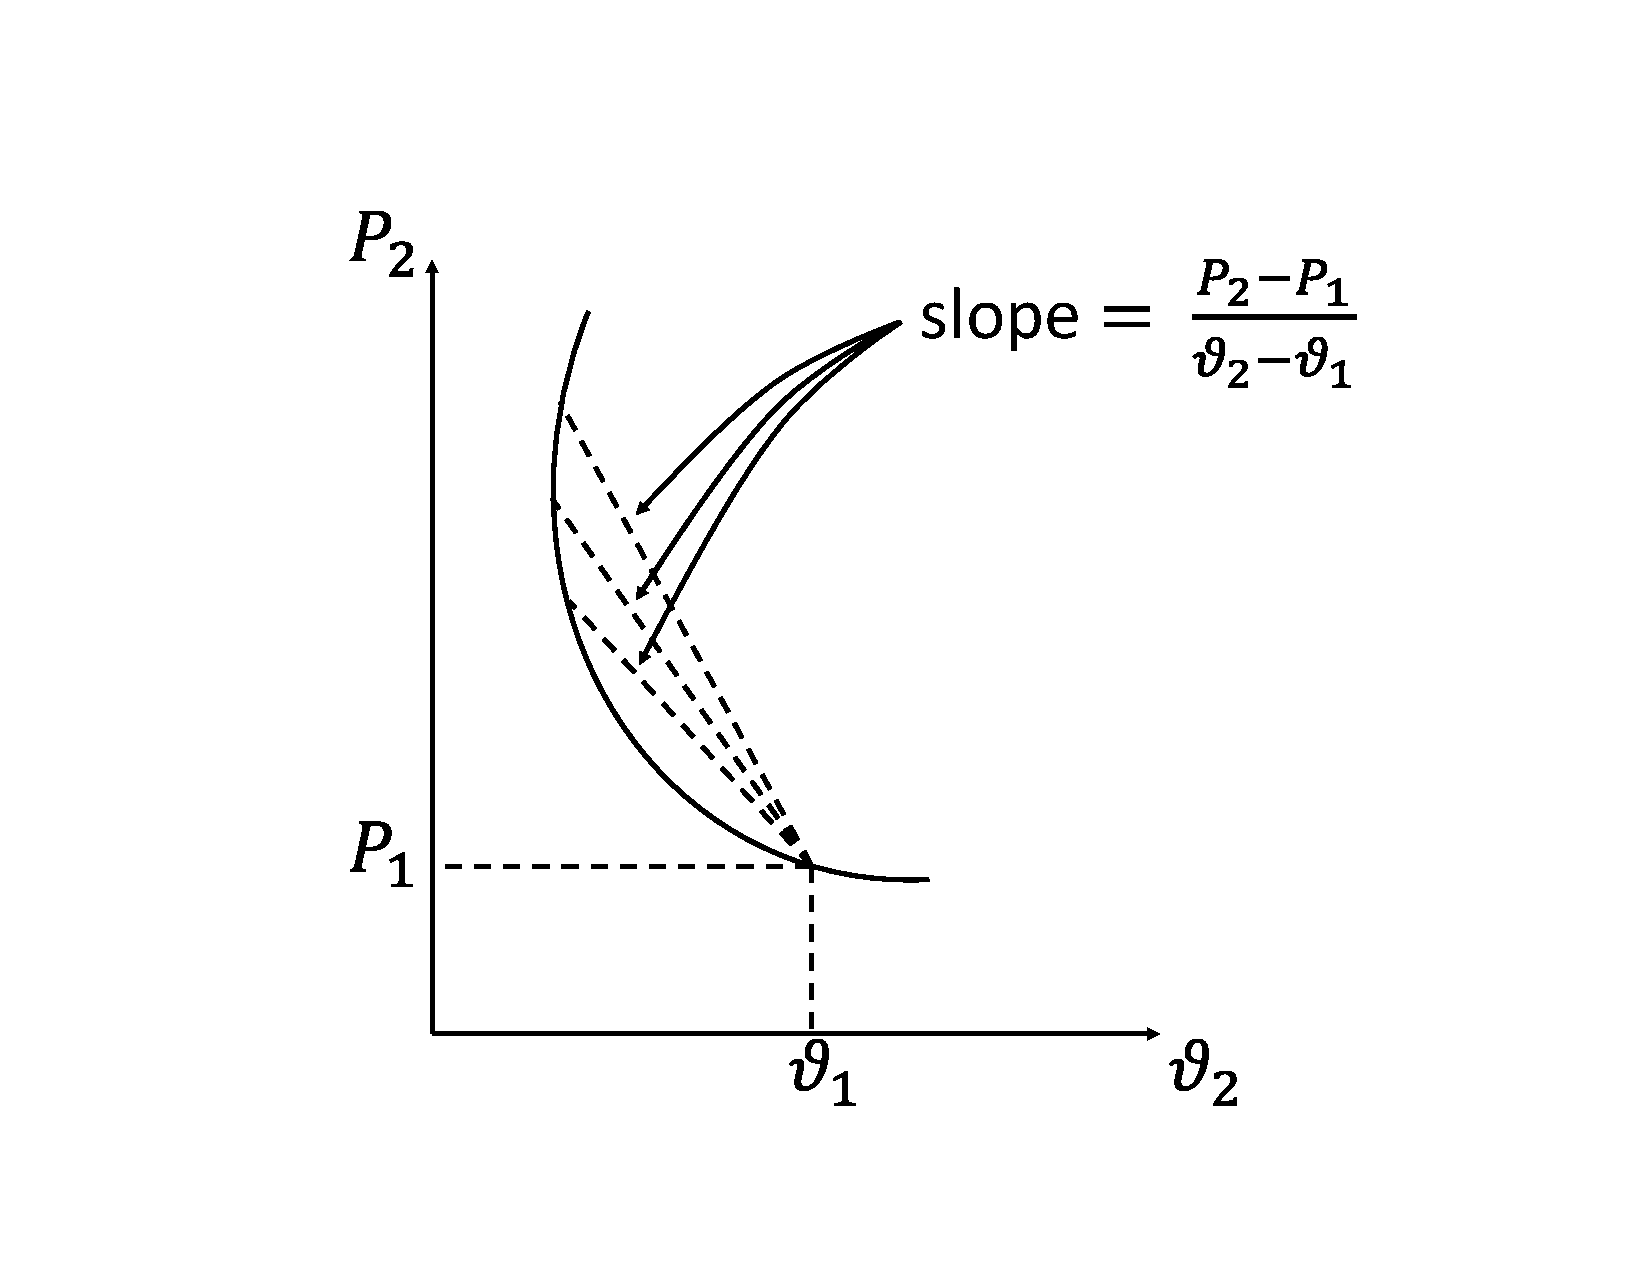
\includegraphics[width=0.7\textwidth]{../images/shock_adiabat.pdf}
   \caption{Shock adiabat for an arbitrary equation of state.}
   \label{fig:shock_adiabat}
\end{figure}

A few extra notes on shock waves:
\begin{itemize}
    \item The shock Mach number $M_{1n}$ is defined as
    \begin{equation}
        M_{1n} = \frac{w_1}{c_1}.
    \end{equation}
    
    \item The speed of sound is independent of the reference frame. Thus, whether you are in the shock reference frame, or in a stationary reference frame, the speeds of sound before and after the shock are invariant.
    
    \item The relative velocities satisfy
    \begin{align}
        w_1 \ge &c_1 \nonumber \\
        w_2 \le &c_2.
    \end{align}
    
    \item The shock strength $\Pi$ is defined as (see \cite{thompson1988} for derivation):
    \begin{equation}
    \label{eq:shock_strength}
        \Pi = \frac{P_2 - P_1}{\rho_1 c_1^2}.
    \end{equation}
    
    \item Strong and weak shocks are defined according to
    \begin{align}
    \label{eq:strong_weak_shocks}
        \Pi \ll 1 \quad & \text{weak shock} \nonumber \\
        \Pi \gg 1 \quad & \text{strong shock}.
    \end{align}
    
    \item For weak shocks the entropy increase across a shock is so weak, they might as well be considered isentropic.
    
    \item In the limit of vanishing strength, shock waves become acoustic discontinuities, propagating with speed $c$ relative to the fluid.
\end{itemize}

%---------------------------------
\subsection{Normal shocks}
%---------------------------------
Following the derivations in \cite{thompson1988} for a perfect gas, one can express shock jump conditions as a function of $\gamma$ and $M_{1n}$ only. These are
\begin{equation}
\label{eq:normal_shock_pressure}
    \frac{P_2}{P_1} = \dfrac{\dfrac{2 \gamma}{\gamma - 1} M_{1n}^2 - 1}{\dfrac{\gamma + 1}{\gamma-1}},
\end{equation}
\begin{equation}
\label{eq:normal_shock_velocity}
    \frac{w_2}{w_1} = \dfrac{1 + \dfrac{\gamma - 1}{2} M_{1n}^2}{\dfrac{\gamma + 1}{2} M_{1n}^2},
\end{equation}
\begin{equation}
\label{eq:normal_shock_density}
    \frac{\rho_2}{\rho_1} = \dfrac{\dfrac{\gamma + 1}{2} M_{1n}^2}{1 + \dfrac{\gamma - 1}{2} M_{1n}^2}.
\end{equation}
Additionally, combining the three above one obtains
\begin{equation}
\label{eq:normal_shock_mach}
    M_{2n}^2 = \dfrac{M_{1n}^2 + \dfrac{2}{\gamma - 1}}{ \dfrac{2\gamma}{\gamma - 1}M_{1n}^2 - 1}.
\end{equation}

According to \cref{eq:shock_jump_energy} $h_{t2} = h_{t1}$ (this holds not only for normal shocks but all shocks). Thus, $T_{t2} = T_{t1}$. For the stagnation pressure, we have
\begin{equation}
\frac{P_{t2}}{P_{t1}} = \frac{P_{t2}}{P_2} \frac{P_1}{P_{t1}} \frac{P_2}{P_1}.
\end{equation}
Using \cref{eq:stagnation_pressure,eq:normal_shock_pressure,eq:normal_shock_mach}, and rearranging, one obtains
\begin{equation}
\label{eq:normal_shock_stagnation_pressure}
    \frac{P_{t2}}{P_{t1}} = \left ( \dfrac{ \dfrac{\gamma + 1}{\gamma - 1} }{ \dfrac{2 \gamma}{\gamma - 1} M_{1n}^2 - 1} \right) ^{ 1 / (\gamma - 1) } \left ( \dfrac{ \dfrac{\gamma + 1}{2} M_{1n}^2 }{ 1 + \dfrac{\gamma - 1}{2} M_{1n}^2 } \right ) ^{\gamma / (\gamma - 1)}.
\end{equation}
Finally, entropy change across a normal shock is
\begin{equation}
s_2 - s_1 = -R \ln \frac{P_{t2}}{P_{t1}},
\end{equation}
as shown in \cite{thompson1988}.

%---------------------------------
\subsection{Oblique shocks}
%---------------------------------
\begin{figure}[ht]
\centering
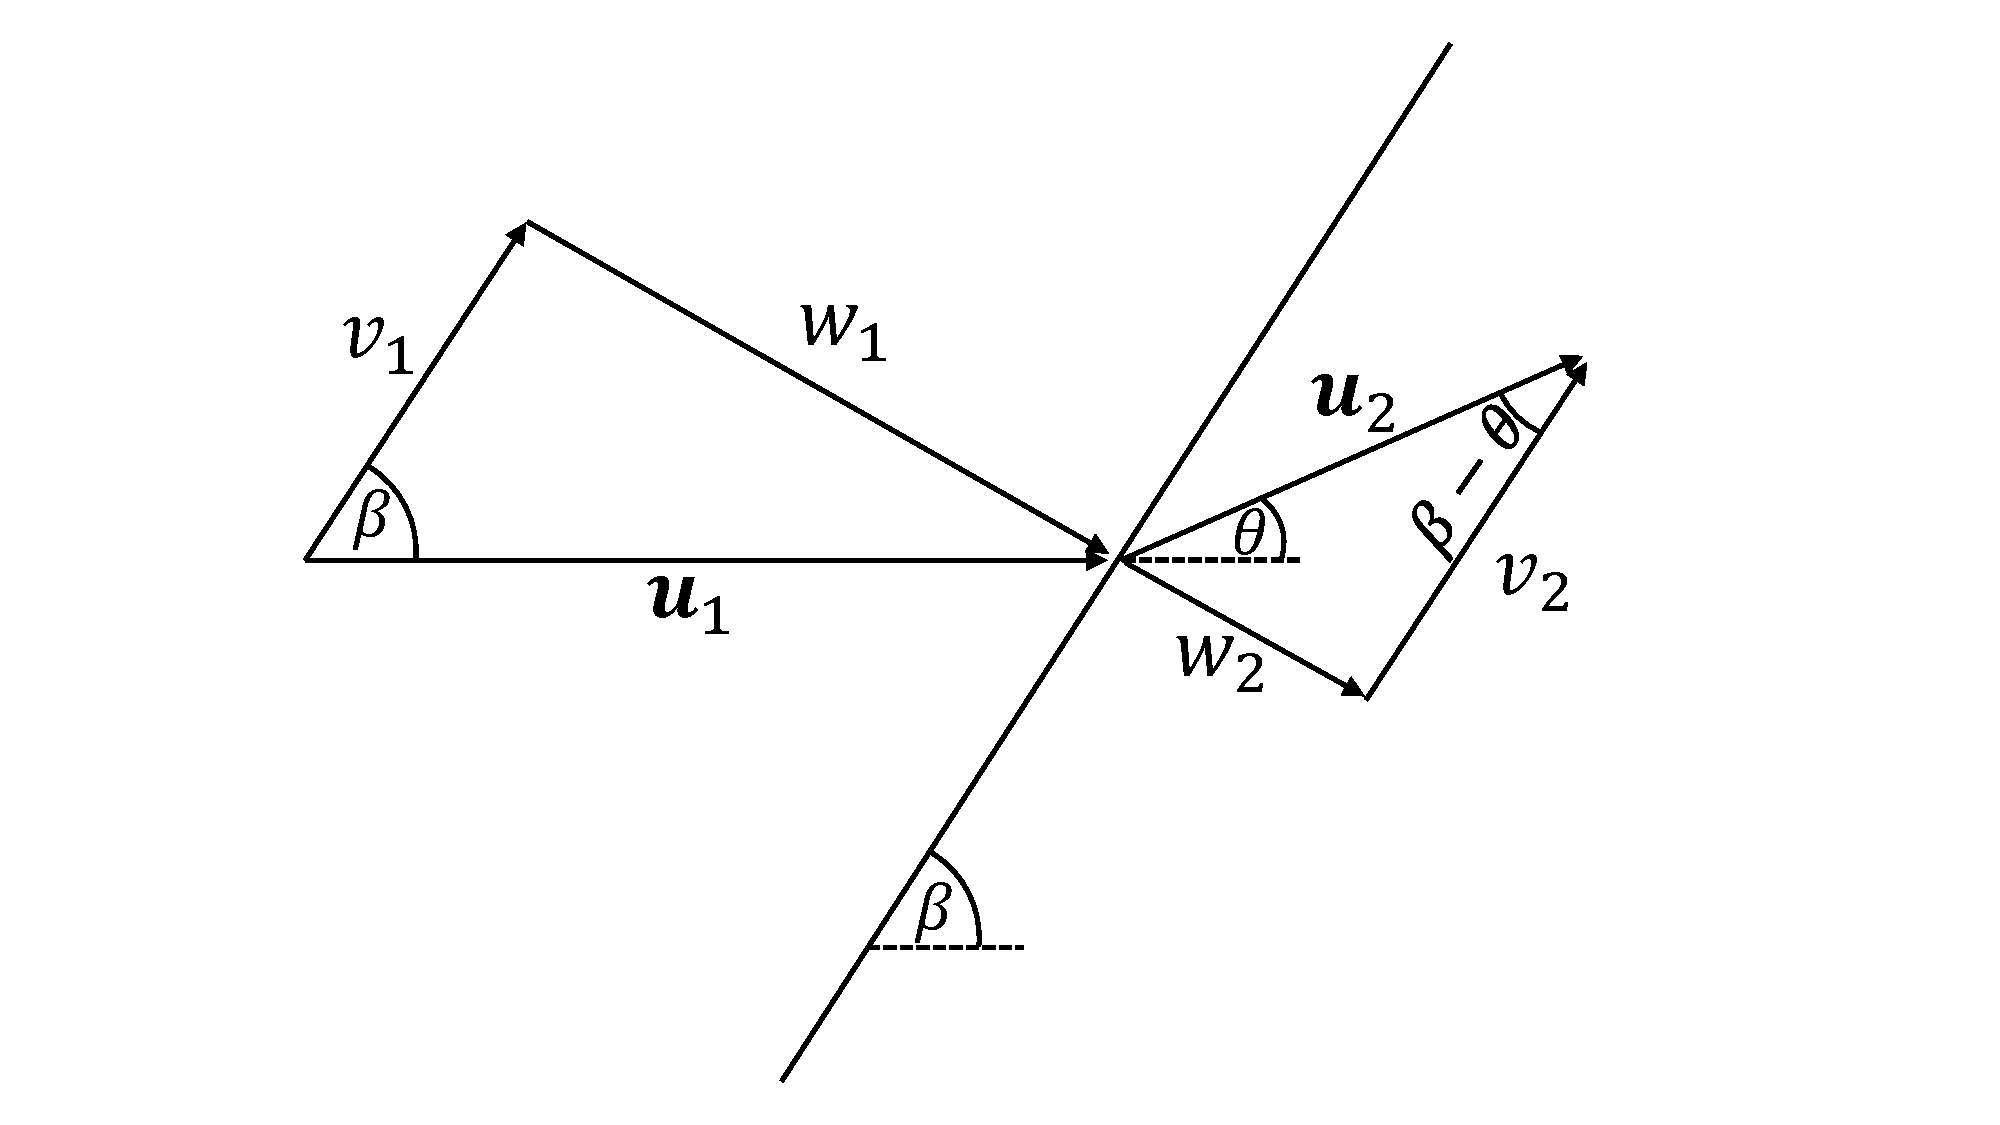
\includegraphics[width=10cm]{../images/oblique_shock.pdf}
\caption{Oblique-shock geometry, $\beta$ is the shock angle and $\theta$ the turning angle.}
\label{fig:oblique_shock}
\end{figure}
The normal shock jump conditions given by \cref{eq:normal_shock_pressure,eq:normal_shock_velocity,eq:normal_shock_density,eq:normal_shock_mach,eq:normal_shock_stagnation_pressure} still apply, but it is again emphasized that $w_1$ and $w_2$ are the components normal to the shock, as defined in \cref{eq:shock_rel_vel_normal}. For the tangential components, defined by \cref{eq:shock_rel_vel_tangential}, we have $v_1 = v_2$ as mentioned in \cref{sec:shock_waves}. As shown in \cref{fig:oblique_shock}, the relationship between $w_1$, $w_2$ and $\uvec_1$, $\uvec_2$ is
\begin{align}
w_1 &= |\uvec_1| \sin{ \beta }, \nonumber \\
w_2 &= |\uvec_2| \sin( \beta - \theta ).
\end{align}
Similarly, the relationship between $v_1$, $v_2$ and $\uvec_1$, $\uvec_2$ is
\begin{align}
v_1 &= |\uvec_1| \cos{ \beta }, \nonumber \\
v_2 &= |\uvec_2| \cos (\beta - \theta).
\end{align}
If the upstream state is known ($\rho_1$, $\uvec_1$, $P_1$, $P_{t1}$), along with the shock angle $\beta$, then the downstream state can be determined using the above relationships and the normal shock jump conditions.

Using the shock jump condition for velocity (\cref{eq:normal_shock_velocity}), and some trigonometric identities, one can derive an equation for $\theta$ in terms of $\beta$, for a given inflow Mach number $M_1 = |\uvec_1|/c_1$, (see \cite{thompson1988}). This relationship is
\begin{equation}
    \tan \theta =\dfrac{ \cot \beta \left ( M_1^2 \sin^2 \beta - 1 \right ) }{ 1 + \left ( \frac{\gamma + 1}{2} \right ) M_1^2 - M_1^2 \sin^2 \beta}.
\end{equation}
The information contained in the above relationship is quite vast, and can best be understood by looking at $\theta$ profiles as a function of $\beta$---for different Mach numbers---obtained from the equation above. A plot of these profiles is given in \cref{fig:theta_beta_1}. Starting from the right-most point on the $x$-axis, labelled as ``a'', is a normal shock with a shock angle of $90^\circ$. Moving along the blue line as the shock angle decreases, we see that the turning angle increases until a maximum, labeled as ``b'', is reached. A further decrease in shock angle leads to point ``c'', which corresponds to turning angles for which the flow behind the shock becomes subsonic. Smaller shock angles lead to even smaller turning angles, until point ``d'' is reached, which corresponds to a Mach wave, to be described in a subsequent section. It is important to note that there are two shock angles that can give the same turning angle. The turning angle corresponding to the smaller shock angle is referred to as the weak solution, whereas the turning angle corresponding to the larger shock angle is the strong solution. This nomenclature has no direct connection to that defined in \cref{eq:strong_weak_shocks}. The black dashed line in \cref{fig:theta_beta_1} corresponds to the peak value for each Mach number, and thus demarcates the weak and strong solutions. A more pictorial representation of this behavior, for the specific case of a shock in front of a cylinder, is given in \cref{fig:theta_beta_2}. 
\begin{figure}[ht]
   \centering
   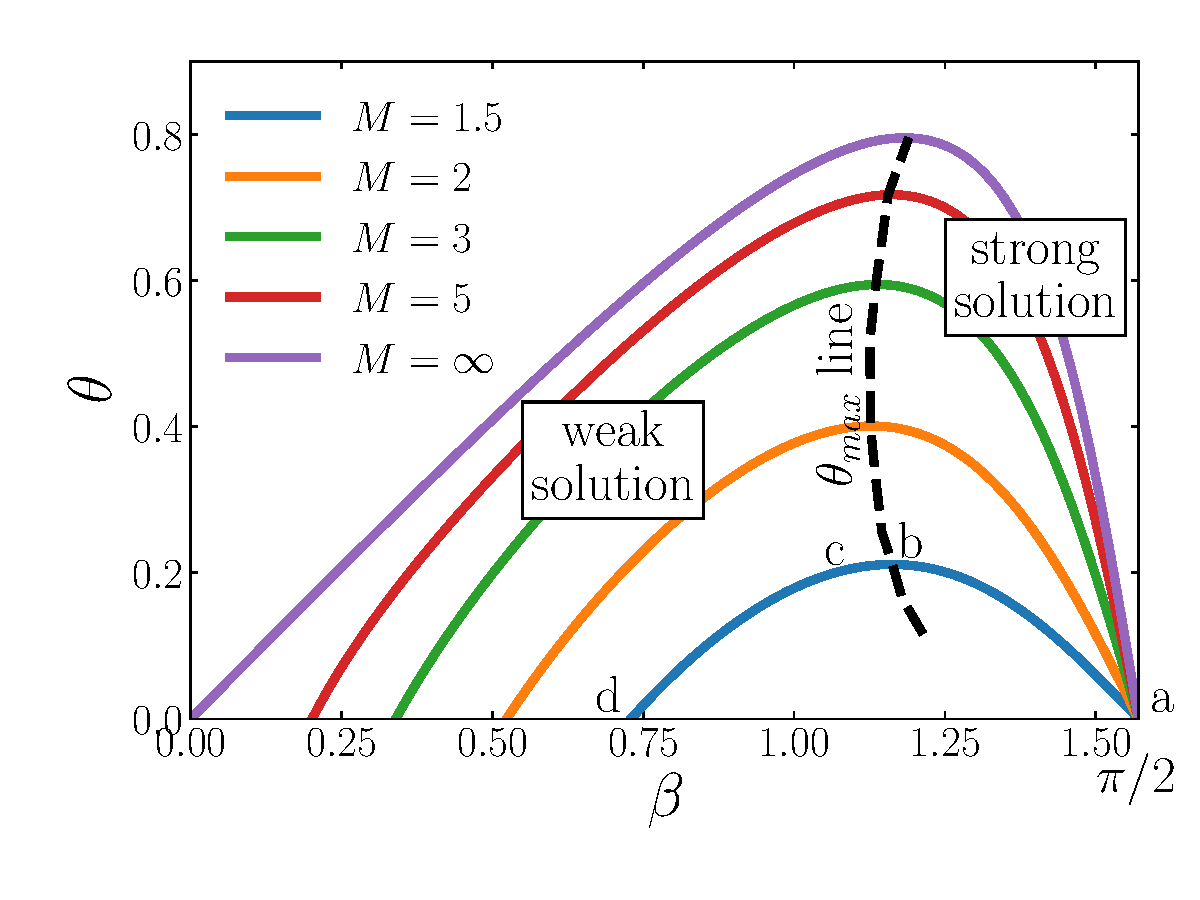
\includegraphics[width=0.5\textwidth]{../images/theta_beta_1.pdf}
   \caption{$\theta$--$\beta$ curve for a perfect gas with $\gamma = 1.4$.}
   \label{fig:theta_beta_1}
\end{figure}

\begin{figure}[ht]
   \centering
   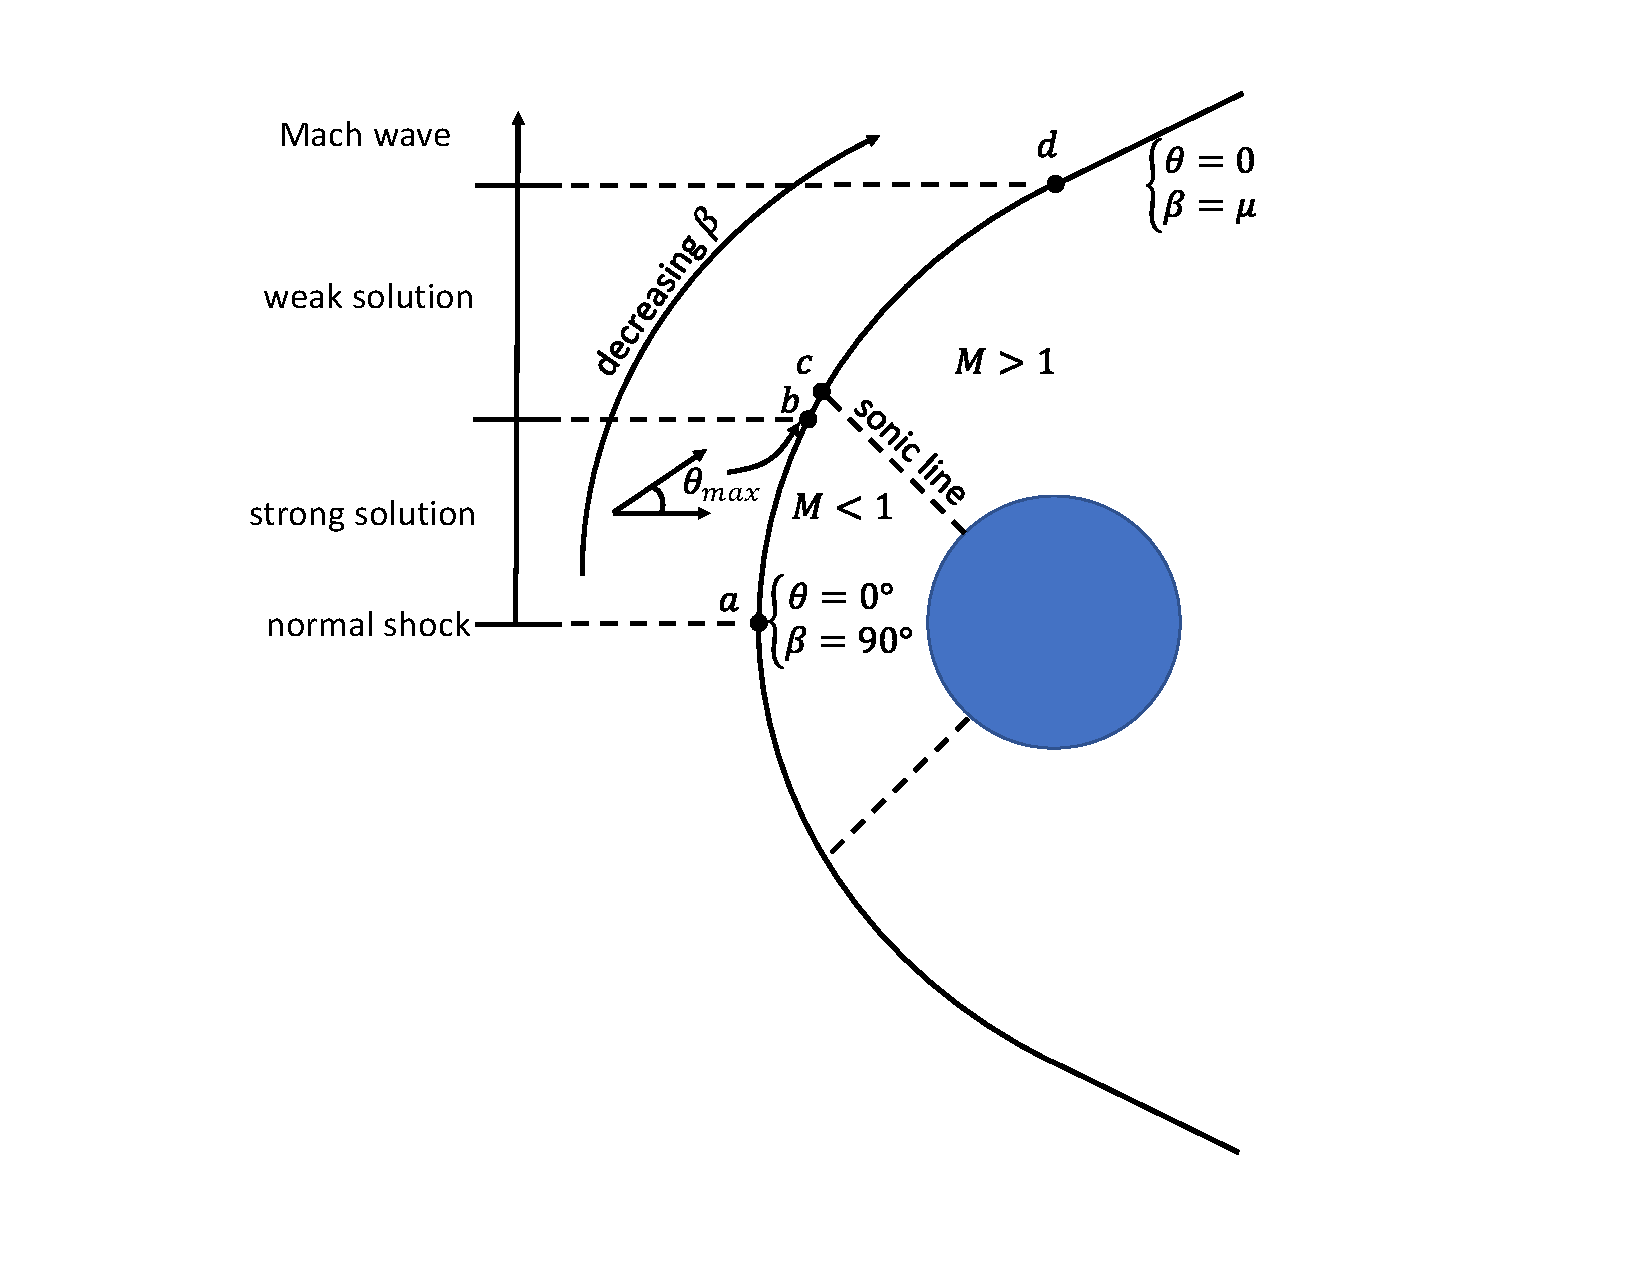
\includegraphics[width=0.7\textwidth]{../images/theta_beta_2.pdf}
   \caption{Representation of different shock waves for different shock angles $\beta$.}
   \label{fig:theta_beta_2}
\end{figure}

Given the information above, it is relevant to ask what happens when a compressible fluid flows over a wedge or a some similar object, whose wedge angle is so large that the turning angle needs to be larger than $\theta_{max}$. Given that, as \cref{fig:theta_beta_1} shows, there is no turning angle greater than $\theta_{max}$, it seems like an inconsistency has been found. In reality, when the flow encounters a wedge whose angle is not that large and the turning angle can be lower than $\theta_{max}$, then the weak solution is the one that occurs and the shock is attached to the leading edge of the wedge. As the wedge angle increases and the flow needs to be deflected by an angle greater than $\theta_{max}$, the shock detaches from the wedge leading edge, as shown in \cref{fig:theta_beta_2}, and both strong and weak solutions occur along the shock. For this case, there will be a section behind the shock that will be subsonic, and thus the flow there can be turned by any angle greater than $\theta_{max}$.

%---------------------------------
\subsection{Weak shocks}
%---------------------------------
By definition, weak shocks are those for which $\Pi$, defined in \cref{eq:shock_strength}, is very small. Assuming that $\rho_1 c_1^2$ is not excessively large, the definition of $\Pi$ indicates that $P_2 - P_1$ is small for weak shocks. We can use the fact that $P_2 - P_1$ is small for weak shocks to show that $(s_2 - s_1) \propto (P_2-P_1)^3$, which then indicates weak shocks have negligible entropy changes.

We begin by adding and subtracting $(P_2 - P_1) \vartheta_1$ on the right-hand side of the Rankine-Hugoniot \cref{eq:rankine_hugoniot} to obtain
\begin{equation}
\label{eq:rankine_hugoniot_vartheta}
    h_2 - h_1 = (P_2 - P_1) \vartheta_1 + \frac{1}{2} (P_2 - P_1) (\vartheta_2 - \vartheta_1).
\end{equation}
We now use Taylor-series expansions for $h$ and $\vartheta$, each as a function of $s$ and $P$, and plug them into the equation above to obtain the scaling of $s$ as a function of $P$. For an arbitrary function $f(s,P)$ the Taylor-series expansion can symbolically be expressed as
\begin{align}
    f_2 - f_1 = &\left [ (s_2 - s_1) \left ( \frac{\partial}{\partial s} \right)_1 + (P_1 - P_1) \left( \frac{\partial}{\partial P} \right)_1 \right ] f \nonumber \\
    + \frac{1}{2! } &\left [ (s_2 - s_1) \left ( \frac{\partial}{\partial s} \right)_1 + (P_1 - P_1) \left( \frac{\partial}{\partial P} \right)_1 \right ]^2 f \nonumber \\
    + \frac{1}{3!}  &\left [ (s_2 - s_1) \left ( \frac{\partial}{\partial s} \right)_1 + (P_1 - P_1) \left( \frac{\partial}{\partial P} \right)_1 \right ]^3 f + ...\nonumber
\end{align}
Since we are interested in the leading-order expression for $(s_2 - s_1)$, terms of higher-order than $(s_2 - s_1)$ will be neglected, i.e. $(s_2 - s_1)^2$, $(s_2 - s_1)^3$, $(s_2 - s_1) (P_2 - P_1)$, etc. 

The Taylor-series expansion for enthalpy is
\begin{equation}
    h_2 - h_1 = (s_2 - s_1) \left ( \frac{\partial h}{\partial s} \right)_1 + (P_2 - P_1) \left ( \frac{\partial h}{\partial P} \right)_1 + \frac{1}{2} (P_2 - P_1)^2 \left( \frac{\partial^2 h}{\partial P^2} \right)_1 + \frac{1}{6}  (P_2 - P_1)^3 \left ( \frac{\partial^3 h}{\partial P^3} \right)_1 + ...
\end{equation}
Using the Gibbs equation shown in \cref{eq:gibbs_form_2}, we have $(\partial h / \partial s)_p = T$ and $(\partial h/ \partial P)_s = \vartheta$. Using this in the above gives
\begin{equation}
    h_2 - h_1 = (s_2 - s_1) T_1 + (P_2 - P_1) \vartheta_1 + \frac{1}{2} (P_2 - P_1)^2 \left( \frac{\partial \vartheta}{\partial P} \right)_1 + \frac{1}{6}  (P_2 - P_1)^3 \left ( \frac{\partial^2 \vartheta}{\partial P^2} \right)_1 + ...
\end{equation}
The Taylor-series expansion for the specific volume is
\begin{equation}
    \vartheta_2 - \vartheta_1 = (s_2 - s_1) \left ( \frac{\partial \vartheta}{\partial s} \right)_1 + (P_2 - P_1) \left ( \frac{\partial \vartheta}{\partial P} \right)_1 + \frac{1}{2} (P_2 - P_1)^2 \left( \frac{\partial^2 \vartheta}{\partial P^2} \right)_1 + \frac{1}{6}  (P_2 - P_1)^3 \left ( \frac{\partial^3 \vartheta}{\partial P^3} \right)_1 + ...    
\end{equation}
Plugging in the two Taylor-series expansions above in \cref{eq:rankine_hugoniot_vartheta}, gives
\begin{multline}
(s_2 - s_1) T_1 + (P_2 - P_1) \vartheta_1 + \frac{1}{2} (P_2 - P_1)^2 \left( \frac{\partial \vartheta}{\partial P} \right)_1 + \frac{1}{6}  (P_2 - P_1)^3 \left ( \frac{\partial^2 \vartheta}{\partial P^2} \right)_1 =\\
(P_2 - P_1) \vartheta_1 + \frac{1}{2} (P_2 - P_1)^2 \left ( \frac{\partial \vartheta}{\partial P} \right)_1 + \frac{1}{4} (P_2 - P_1)^3 \left ( \frac{\partial^2 \vartheta}{\partial P^2} \right)_1 + ...
\end{multline}
Simplifying the above finally gives
\begin{equation}
    s_2 - s_1 = \frac{1}{12 T_1} \left ( \frac{\partial^2 \vartheta}{\partial P^2} \right)_1 (P_2 - P_1)^3 + ...
\end{equation}
that is, $(s_2 - s_1) \propto (P_2-P_1)^3$.

%---------------------------------
\subsection{Strong shocks}
%---------------------------------
Strong shocks are defined as those for which $\Pi \gg 1$. In general, it seems that $P < \rho c^2$, and thus
\begin{equation}
    \Pi =  \frac{P_2}{\rho_1 c_1^2} - \frac{P_1}{\rho_1 c_1^2} \gg 1
\end{equation}
becomes
\begin{equation}
    \frac{P_2}{\rho_1 c_1^2}  \gg 1,
\end{equation}
or
\begin{equation}
    P_2 \gg \rho_1 c_1^2.
\end{equation}
The above in turn implies $P_2 \gg P_1$, that is, $P_1$ is negligible.

Consider the normal shock jump condition for pressure given by \cref{eq:normal_shock_pressure}. It can be rearranged to give
\begin{equation}
P_2 = \dfrac{ \dfrac{2 \gamma}{\gamma - 1} \dfrac{\rho_1 w_1^2}{\gamma} - P_1}{\dfrac{\gamma + 1}{\gamma - 1}}.
\end{equation}
Since $P_1$ can be neglected, this gives
\begin{equation}
\label{eq:normal_shock_pressure_strong}
    P_2 = \frac{2}{\gamma + 1} \rho_1 w_1^2.
\end{equation}
Additionally, since $M_{1n}^2 = \rho_1 w_1^2 / \gamma P_1$, a negligible $P_1$ leads to $M_{1n}^2 \gg 1$. Thus, \cref{eq:normal_shock_velocity,eq:normal_shock_density,eq:normal_shock_mach} give
\begin{equation}
\label{eq:normal_shock_velocity_strong}
    \frac{w_2}{w_1} = \frac{\gamma -1}{\gamma + 1},
\end{equation}
\begin{equation}
\label{eq:normal_shock_density_strong}
    \frac{\rho_2}{\rho_1} = \frac{\gamma + 1}{\gamma -1},
\end{equation}
and
\begin{equation}
\label{eq:normal_shock_mach_strong}
    M_{2n}^2 = \frac{\gamma - 1}{2\gamma}.
\end{equation}


%------------------------------------------------------------------------
\section{Mach Waves}
%------------------------------------------------------------------------

\begin{figure}[ht]
\centering
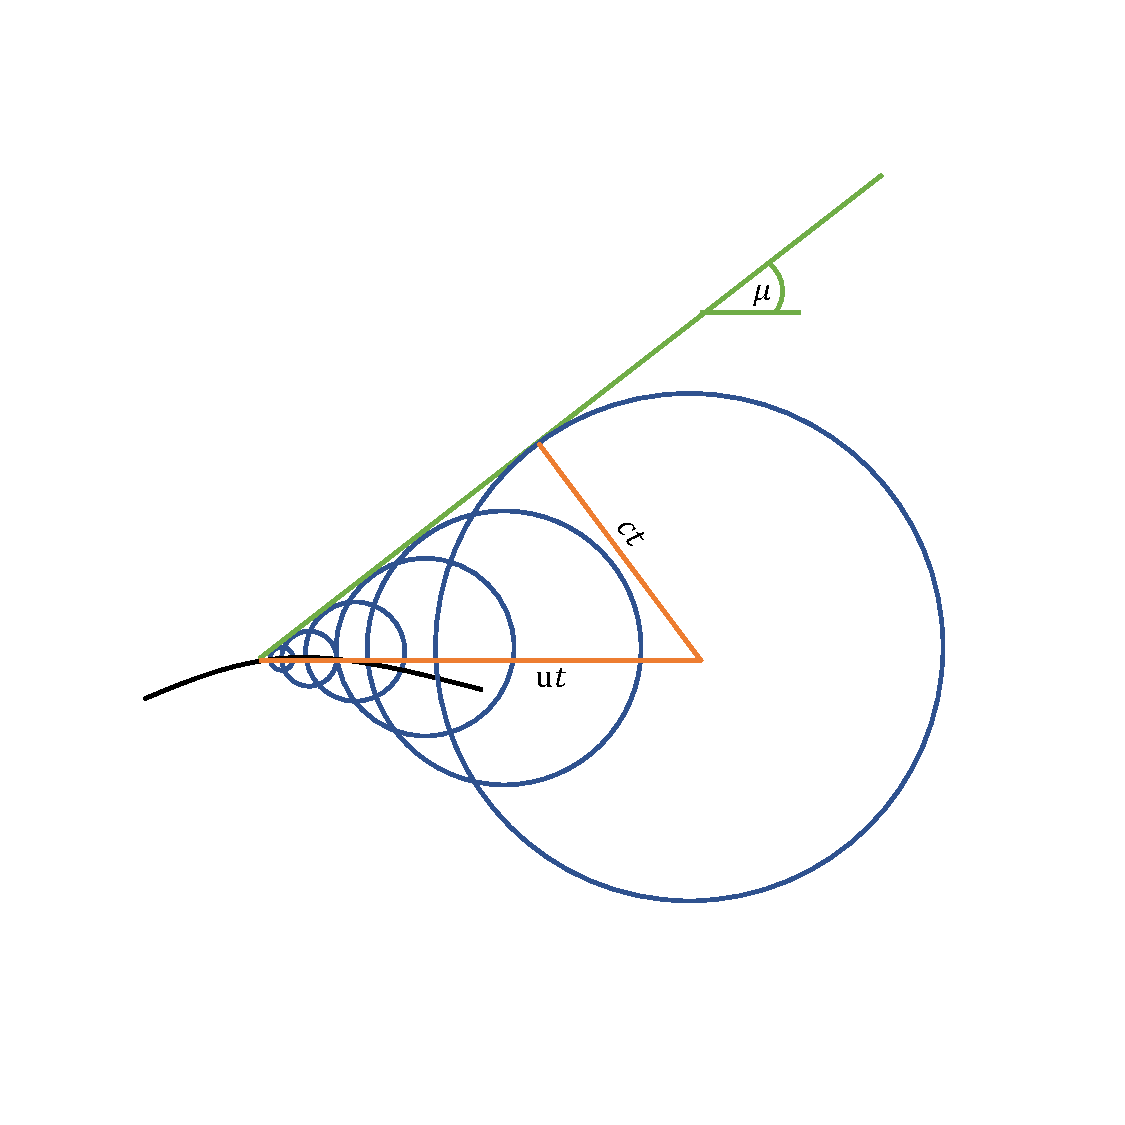
\includegraphics[width=8cm]{../images/mach_wave.pdf}
\caption{Mach wave}
\label{fig:mach_wave}
\end{figure}
Assume a vehicle is moving at a Mach number greater than one. In \cref{fig:mach_wave}, the black line represents a section of the surface of the vehicle moving at supersonic speeds. At each instance in time, each infinitesimal point on this surface slightly distorts the stationary fluid and thus produces acoustic waves (blue line). These waves, by definition, expand at the speed of sound. The green line, which is aligned with the front of the acoustic waves, is referred to as a Mach wave or Mach line. The angle of inclination of this Mach wave, labeled $\mu$, is called the Mach angle and satisfies
\begin{equation}
    \sin (\mu) = \frac{1}{M}.
\end{equation}


%------------------------------------------------------------------------
\section{Contact discontinuities}
%------------------------------------------------------------------------
A contact discontinuity is defined as a surface that separates two fluids of different properties or at different states. A defining condition is that there is no flow of matter across a contact discontinuity, that is, $w_1 = w_2 = 0$. Using this in the integral momentum conservation equation for a thin box bounding the discontinuity, and assuming negligible viscous stresses and heat fluxes, leads to $P_1 = P_2$. However, other flow properties, such as $\rho$, $T$, and $v$ can change across the discontinuity.

%########################################################################
\chapter{Quasi 1-D steady and unsteady flow}
%########################################################################
Quasi 1-D eqs; mass balance, f(M), and PAFMT; Fanno flow, Rayleigh flow.

%########################################################################
Local acoustic speed, Expansion and Compression wave, Shock tube.

%########################################################################
\chapter{2-D Compressible flow}
%########################################################################
Prandtl-Meyer (Compressive, Expansive); Shock-Expansion Theory: 2D Airfoil Calculations, Shock Reflection, Isentropic flow in curved channel, Nozzle exit flows.

%########################################################################
\chapter{Hydrodynamic Instabilities}
%########################################################################

%------------------------------------------------------------------------
\section{Linear Stability}
%------------------------------------------------------------------------
Consider the following system of PDEs for a two-dimensional problem
\begin{equation}
    \frac{\partial w}{\partial t} = \frac{\partial \phi}{\partial y}\frac{\partial w}{\partial x} - \frac{\partial \phi}{\partial x} \frac{\partial w}{\partial y},
\end{equation}
\begin{equation}
    w = \nabla^2 \phi .
\end{equation}
In the above, $\phi = \phi(x,y,t)$ is the electrostatic potential and $w = w(x,y,t)$ the vorticity.

The analysis begins by splitting the variables into equilibrium and fluctuating components, namely
\begin{equation}
    \phi = \phi_0 + \phi_1,
\end{equation}
\begin{equation}
    w = w_0 + w_1.
\end{equation}
For the above, $\phi_0 = \phi_0(x)$, $w_0 = w_0(x)$, and $\phi_1 = \phi_1(x,y,t)$, $w_1 = w_1(x,y,t)$. We now introduce a Fourier series decomposition for the fluctuating variables, and focus on a single Fourier mode as follows 
\begin{equation}
    \phi_1(x,y,t) = F(x,k_y,t) e^{ik_y y} = \tilde{\phi}(x,k_y) e^{\gamma t + i k_y y},
\end{equation}
\begin{equation}
    w_1(x,y,t) = G(x,k_y,t) e^{ik_y y} = \tilde{w}(x,k_y) e^{\gamma t + i k_y y}.
\end{equation}
In the above, $\gamma$, which can be complex, is the growth rate factor, and $\tilde{\phi} = \tilde{\phi}(x, k_y)$, $\tilde{w} = \tilde{w}(x, k_y)$ are the remaining part of the Fourier coefficient.

We then plug in the decompositions for $\phi$ and $w$ in the governing PDEs. Collecting the lowest order terms leads to equations for the equilibrium solution. For example, the Poisson equation to lowest order is
\begin{equation}
    \label{eq:lin_stab_w0_phi0}
    w_0 = \nabla^2 \phi_0 = \frac{\partial^2 \phi_0}{\partial x^2}.
\end{equation}
Combining terms up to next order gives
\begin{equation}
    \label{eq:lin_stab_pde_mid_order}
    \frac{\partial w_1}{\partial t} = \frac{\partial \phi_0}{\partial y}\frac{\partial w_1}{\partial x} + \frac{\partial \phi_1}{\partial y}\frac{\partial w_0}{\partial x} - \frac{\partial \phi_0}{\partial x} \frac{\partial w_1}{\partial y} - \frac{\partial \phi_1}{\partial x} \frac{\partial w_0}{\partial y},
\end{equation}
\begin{equation}
    w_1 = \nabla^2 \phi_1.
\end{equation}
Using the expression for $\phi_1$ in the Poisson equation above leads to 
\begin{equation}
    w_1 = \left ( \frac{\partial^2 \tilde{\phi}}{\partial x^2} - k_y^2 \tilde{\phi} \right ) e^{\gamma t + i k_y y},
\end{equation}
or 
\begin{equation}
    \tilde{w} = \frac{\partial^2 \tilde{\phi}}{\partial x^2} - k_y^2 \tilde{\phi} .
\end{equation}
We'll now evaluate each of the terms in \cref{eq:lin_stab_pde_mid_order}.
\begin{align}
    \frac{\partial w_1}{\partial t} &= \gamma \left ( \frac{\partial^2 \tilde{\phi}}{\partial x^2} - k_y^2 \tilde{\phi} \right ) e^{\gamma t + i k_y y}, \nonumber \\
    \frac{\partial \phi_0}{\partial y}\frac{\partial w_1}{\partial x} &= 0, \nonumber \\
    \frac{\partial \phi_1}{\partial y}\frac{\partial w_0}{\partial x} &= i k_y \tilde{\phi} e^{\gamma t + i k_y y} \frac{\partial^3 \phi_0}{\partial x^3}, \nonumber \\
    \frac{\partial \phi_0}{\partial x} \frac{\partial w_1}{\partial y} &= \frac{\partial \phi_0}{\partial x} i k_y \left ( \frac{\partial^2 \tilde{\phi}}{\partial x^2} - k_y^2 \tilde{\phi} \right ) e^{\gamma t + i k_y y},\nonumber \\
    \frac{\partial \phi_1}{\partial x} \frac{\partial w_0}{\partial y} &= 0 . \nonumber \\
\end{align}
Combining all of the above, we obtain
\begin{equation}
    \gamma \left ( \frac{\partial^2 \tilde{\phi}}{\partial x^2} - k_y^2 \tilde{\phi} \right ) = ik_y \tilde{\phi} \frac{\partial^3 \phi_0}{\partial x^3} - \frac{\partial \phi_0}{\partial x} i k_y \left ( \frac{\partial^2 \tilde{\phi}}{\partial x^2} - k_y^2 \tilde{\phi} \right ).
\end{equation}
This is re-written as 
\begin{equation}
    \gamma \left ( \frac{\partial^2 \tilde{\phi}}{\partial x^2} - k_y^2 \tilde{\phi} \right ) = -i k_y \left [ \frac{\partial \phi_0}{\partial x} \left ( \frac{\partial^2 \tilde{\phi}}{\partial x^2} - k_y^2 \tilde{\phi} \right ) - \frac{\partial^3 \phi_0}{\partial x^3} \tilde{\phi} \right ].
\end{equation}

%%%%%%%%%%%%%%%%%%%%%%%%%%%%%%%%%%%%%%%%%%%%%%%%%%%%%%%%%%%%%%%%%%%%%%%%%
\part{Magnetic Fields}
%%%%%%%%%%%%%%%%%%%%%%%%%%%%%%%%%%%%%%%%%%%%%%%%%%%%%%%%%%%%%%%%%%%%%%%%%

%########################################################################
\chapter{Guiding center theory}
%########################################################################
We begin with the velocity equation for a particle under the action of electric and magnetic fields, 
\begin{equation}
\label{eq:single_particle_motion}
    m \frac{d \vvec}{dt} = e \left ( \Evec + \vvec \times \Bvec \right )_{\qvec = \xvec}.
\end{equation}
In the above, $\vvec = \vvec(t)$ is the particle velocity, $\xvec = \xvec(t)$ the particle position, $\Evec = \Evec(\qvec,t)$ the electric field, and $\Bvec = \Bvec(\qvec,t)$ the magnetic field. In the subsections that follow, we will solve this equation of motion for simplified forms of $\Evec$ and $\Bvec$. The solutions for the velocity vector will typically be of the form
\begin{equation}
    \label{eq:single_particle_motion_vel_general}
    \vvec = \vvec^{(c)} + \vvec^{(g)} + v^{||} \bvec,
\end{equation}
where $\vvec^{(c)} = \vvec^{(c)}(t)$ is the gyromotion (cyclotron) velocity, $\vvec^{(g)} = \vvec^{(g)}(t)$ is the guiding center velocity, $v^{||} = v^{||}(t)$ is the parallel velocity. Not all of the velocities will always be present. $\bvec = \Bvec / B$ is the unit magnetic field vector. The position of the particle is governed by 
\begin{equation}
    \frac{d\xvec}{dt} = \vvec.
\end{equation}
Using \cref{eq:single_particle_motion_vel_general}, we integrate the above to obtain
\begin{equation}
    \label{eq:single_particle_motion_pos_eq_mod}
    \int_0^t \, d\xvec(t') = \int_0^t \vvec^{(c)}(t') \, dt' + \int_0^t \vvec^{(g)}(t') \, dt' + \int_0^t v^{||}(t) \bvec \, dt'.
\end{equation}
We introduce the positions $\xvec^{(c)} = \xvec^{(c)}(t)$, $\xvec^{(g)} = \xvec^{(g)}(t)$, and $\xvec^{||} = \xvec^{||}(t)$, which are defined as follows
\begin{equation}
    \xvec^{(c)} = \int \vvec^{(c)} \, dt,
\end{equation}
\begin{equation}
    \xvec^{(g)} = \int \vvec^{(g)} \, dt,
\end{equation}
\begin{equation}
    \xvec^{||} = \int v^{||} \bvec \, dt.
\end{equation}
Thus, \cref{eq:single_particle_motion_pos_eq_mod} is now re-written as
\begin{equation}
    \xvec(t) - \xvec(0) = \xvec^{(c)}(t) - \xvec^{(c)}(0) + \xvec^{(g)}(t) - \xvec^{(g)}(0) - \xvec^{||}(t) - \xvec^{||}(0).
\end{equation}
Without loss of generality, we will assume that the initial condition is as follows
\begin{equation}
    \xvec(0) = \xvec^{(c)}(0) + \xvec^{(g)}(0) + \xvec^{||}(0).
\end{equation}
Thus, the particle position is finally expressed as
\begin{equation}
    \label{eq:single_particle_motion_pos_general}
    \xvec = \xvec^{(c)} + \xvec^{(g)} + \xvec^{||}.
\end{equation}


 
%------------------------------------------------------------------------
\section{Uniform $\Evec$ and $\Bvec$ fields}
%------------------------------------------------------------------------

%--------------------------------------------
\subsection{Only $\Evec$ field}
%--------------------------------------------
Let's orient our coordinate system such that $\Evec$ points in the $\evec_z$ direction. Thus, the equations of motion are
\begin{alignat}{2}
    &\frac{d v_x}{dt} = 0  \qquad && v_x(0) = v_\perp \cos(\phi), \nonumber \\
    &\frac{d v_y}{dt} = 0  \qquad && v_y(0) = v_\perp \sin(\phi), \nonumber \\
    &\frac{d v_z}{dt} = \frac{e E}{m}  \qquad && v_z(0) = v_{||}.
\end{alignat}
The solution of the above is
\begin{align}
    v_x &= v_\perp \cos(\phi) \nonumber \\
    v_y &= v_\perp \sin(\phi) \nonumber \\
    v_z &= v_{||} + \frac{e E}{m} t.
\end{align}


%--------------------------------------------
\subsection{Only $\Bvec$ field}
%--------------------------------------------
\begin{figure}[ht]
    \centering
    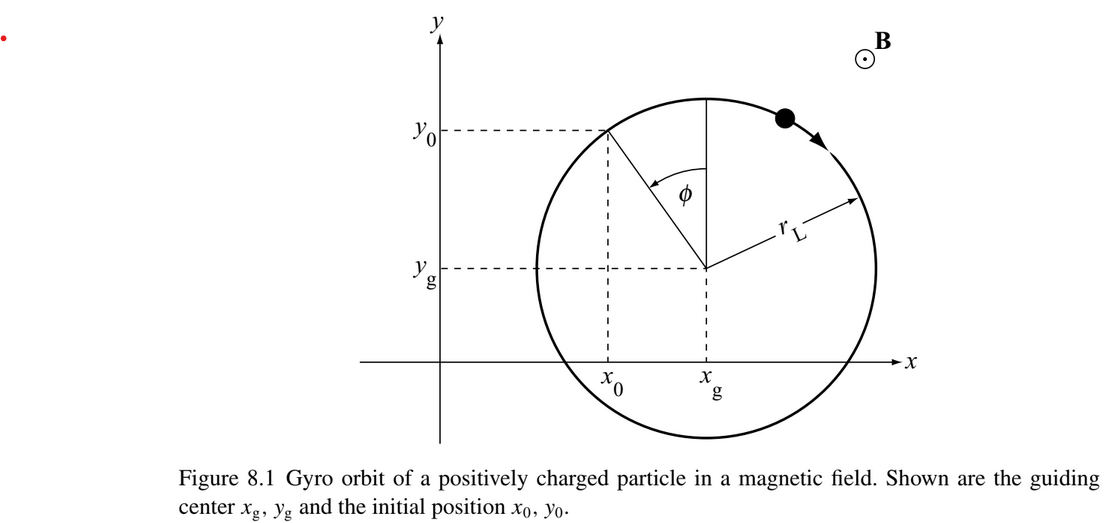
\includegraphics[width=\textwidth]{../images/gyromotion_coordinates.png}
    \caption{Coordinates for gyromotion (extracted from Plasma Physics and Fusion Energy, J. P. Freidberg).}
    \label{fig:gyromotion_coordiantes}
\end{figure}

\label{sec:only_B_field}
Let's orient our coordinate system such that $\Bvec$ points in the $\evec_z$ direction. Thus, the equations of motion are
\begin{subequations}
\begin{alignat}{2}
    &\frac{d v_x}{dt} = \frac{eB}{m} v_y  \qquad && v_x(0) = v_\perp \cos(\phi), \label{eq:only_B_1} \\
    &\frac{d v_y}{dt} = -\frac{eB}{m} v_x  \qquad && v_y(0) = v_\perp \sin(\phi), \label{eq:only_B_2} \\
    &\frac{d v_z}{dt} = 0  \qquad && v_z(0) = v_{||}. \label{eq:only_B_3}
\end{alignat}
\end{subequations}
The $z$ component is decoupled from the rest and has a trivial solution. For the other two components, we begin by taking the time derivative of \cref{eq:only_B_2}. Thus
\begin{equation}
    \frac{d^2 v_y}{dt^2} = -\frac{eB}{m} \frac{d v_x}{dt} = -w_c^2 v_y,
\end{equation}
where $w_c = |e|B/m$ is the gyro frequency. We know that the general solution to the above is $v_y = c_1 \cos(w_c t) + c_2 \sin(w_c t)$. If we use the ICs and assume ions, we have
\begin{equation}
\label{eq:vel_gyro_y}
    v_y = -v_\perp \sin(w_ct - \phi).
\end{equation}
Integrating \cref{eq:only_B_1} then gives
\begin{equation}
\label{eq:vel_gyro_x}
    v_x = v_\perp \cos(w_c t - \phi).
\end{equation}
The final solution, for either positive or negative charges, can be written as
\begin{align}
\label{eq:vel_gyro}
    v^{(c)}_x &= v_\perp \cos(w_c t \pm \phi) \nonumber \\
    v^{(c)}_y &= \pm v_\perp \sin(w_c t \pm \phi),
\end{align}
where upper signs correspond to a negative charge. Integrating the equations above leads to
\begin{align}
\label{eq:pos_gyro}
    x^{(c)} &= r_L \sin(w_c t \pm \phi) \nonumber \\
    y^{(c)} &= \mp r_L \cos(w_c t \pm \phi).
\end{align}
where $r_L = v_\perp/w_c$ is the gyro radius.

%--------------------------------------------
\subsection{Both $\Evec$ and $\Bvec$ fields}
%--------------------------------------------
\label{sec:E_and_B_field}
Let's orient our coordinate system such that $\Bvec$ still points along $\evec_z$. The equations of motion are
\begin{subequations}
\label{eq:single_particle_motion_EcrossB_temp1}
\begin{alignat}{2}
    &\frac{d v_x}{dt} = \frac{eE_x}{m} + \frac{eB}{m} v_y  \qquad && v_x(0) = v_\perp \cos(\phi) + \frac{E_y}{B}, \label{eq:E_and_B_1} \\
    &\frac{d v_y}{dt} = \frac{eE_y}{m} - \frac{eB}{m} v_x  \qquad && v_y(0) = v_\perp \sin(\phi) - \frac{E_x}{B}, \label{eq:E_and_B_2} \\
    &\frac{d v_z}{dt} = \frac{e E_{||}}{m}  \qquad && v_z(0) = v_{||}, \label{eq:E_and_B_3}
\end{alignat}
\end{subequations}
where we have chosen the given initial conditions simply to facilitate the math. Again, the z component is decoupled from the rest and has the trivial solution $v_z = v_{||} +  (eE_{||}/m) t$. Thus, \cref{eq:single_particle_motion_vel_general} for the $x$ and $y$ components are
\begin{align}
    \label{eq:single_particle_motion_EcrossB_temp2}
    v_x &= v_x^{(c)} + v^{(g)}_x, \nonumber \\
    v_y &= v_y^{(c)} + v^{(g)}_y.
\end{align}
We assume $v^{(g)}_x$ and $v^{(g)}_y$ are time independent. Using \cref{eq:single_particle_motion_EcrossB_temp2} in \cref{eq:single_particle_motion_EcrossB_temp1} we obtain
\begin{align}
    0 &= \frac{eE_x}{m} + \frac{eB}{m}v^{(g)}_y \nonumber \\
    0 &= \frac{eE_y}{m} - \frac{eB}{m}v^{(g)}_x.
\end{align}
Thus, $v^{(g)}_x = E_y/B$ and $v^{(g)}_y = -E_x/B$, which in vector notation can be expressed as
\begin{equation}
    \vvec^{(g)}_E = \frac{\Evec \times \Bvec}{B^2}.
\end{equation}

%------------------------------------------------------------------------
\section{Non-uniform $\Bvec$ field}
%------------------------------------------------------------------------

%--------------------------------------------
\subsection{Change in magnitude along perpendicular directions}
%--------------------------------------------
The magnetic field still points in the $\evec_z$ direction, but its magnitude changes in directions perpendicular to $\evec_z$: $B = B(q_x,q_y)$. The equations of motion are
\begin{subequations}
\begin{alignat}{2}
    &\frac{d v_x}{dt} = \frac{eB(x,y)}{m} v_y  \qquad && v_x(0) = v_\perp \cos(\phi) -\frac{v^2_\perp}{2 w_c} \left . \frac{\partial B}{\partial q_y} \right |_{x^{(g)},y^{(g)}} \frac{1}{B(x^{(g)},y^{(g)})}, \label{eq:nonuniB_1} \\
    &\frac{d v_y}{dt} = -\frac{eB(x,y)}{m} v_x  \qquad && v_y(0) = v_\perp \sin(\phi) + \frac{v^2_\perp}{2 w_c} \left . \frac{\partial B}{\partial q_x} \right |_{x^{(g)},y^{(g)}} \frac{1}{B(x^{(g)},y^{(g)})}, \label{eq:nonuniB_2} \\
    &\frac{d v_z}{dt} = 0  \qquad && v_z(0) = v_{||}. \label{eq:nonuniB_3}
\end{alignat}
\end{subequations}
In the above, the $x$ and $y$ in $B(x,y)$ are the perpendicular components of the particle's position. The $v_z$ component is decoupled from the rest and has a trivial solution. Thus, \cref{eq:single_particle_motion_vel_general,eq:single_particle_motion_pos_general} for the $x$ and $y$ components are
\begin{equation}
    \label{eq:single_particle_motion_vel_Bmag_change_perp_1}
    v_x = v_x^{(c)} + v_x^{(g)},
\end{equation}
\begin{equation}
    \label{eq:single_particle_motion_vel_Bmag_change_perp_2}
    v_y = v_y^{(c)} + v_y^{(g)},
\end{equation}
\begin{equation}
    \label{eq:single_particle_motion_pos_Bmag_change_perp_1}
    x = x^{(c)} + x^{(g)},
\end{equation}
\begin{equation}
    \label{eq:single_particle_motion_pos_Bmag_change_perp_2}
    y = y^{(c)} + y^{(g)}.
\end{equation}

We begin by employing a Taylor-series expansion for the magnetic field
\begin{equation}
    B(x,y) = B(x^{(g)}, y^{(g)}) + \left . \frac{\partial B}{\partial q_x} \right |_{x^{(g)},y^{(g)}} x^{(c)} + \left . \frac{\partial B}{\partial q_y} \right |_{x^{(g)},y^{(g)}} y^{(c)} + ...
\end{equation}
Thus, \cref{eq:nonuniB_1,eq:nonuniB_2} are now
\begin{equation}
    \frac{ d v_x}{dt} = \frac{e B(x^{(g)},y^{(g)})}{m} v_y + \frac{e}{m} \left ( \left . \frac{\partial B}{\partial q_x} \right|_{x^{(g)},y^{(g)}} x^{(c)} + \left . \frac{\partial B}{\partial q_y} \right |_{x^{(g)},y^{(g)}} y^{(c)} \right) v_y
\end{equation}
\begin{equation}
    \frac{ d v_y}{dt} = -\frac{e B(x^{(g)},y^{(g)})}{m} v_x + \frac{e}{m} \left ( \left . \frac{\partial B}{\partial q_x} \right|_{x^{(g)},y^{(g)}} x^{(c)} + \left . \frac{\partial B}{\partial q_y} \right |_{x^{(g)},y^{(g)}} y^{(c)} \right ) v_x.
\end{equation}
As before, we assume $v_x^{(g)}$, $v_y^{(g)}$ are time independent. Also, for simplicity we assume ions only. Plugging in \cref{eq:single_particle_motion_vel_Bmag_change_perp_1,eq:single_particle_motion_vel_Bmag_change_perp_2} into the above, we get
\begin{equation}
    0 = B(x^{(g)},y^{(g)}) v_y^{(g)} + \left ( \left . \frac{\partial B}{\partial q_x} \right|_{x^{(g)},y^{(g)}} x^{(c)} + \left . \frac{\partial B}{\partial q_y} \right |_{x^{(g)},y^{(g)}} y^{(c)} \right) \left ( v_y^{(c)} + v_y^{(g)} \right),
\end{equation}
\begin{equation}
    0 = -B(x^{(g)},y^{(g)}) v_x^{(g)} + \left ( \left . \frac{\partial B}{\partial q_x} \right|_{x^{(g)},y^{(g)}} x^{(c)} + \left . \frac{\partial B}{\partial q_y} \right |_{x^{(g)},y^{(g)}} y^{(c)} \right ) \left ( v_x^{(c)} + v_x^{(g)} \right ).
\end{equation}
We assume $v_x^{(g)} \ll v_x^{(c)}$ and $v_y^{(g)} \ll v_y^{(c)}$. Thus, the above becomes
\begin{equation}
    \label{eq:single_particle_motion_Bmag_change_perp_temp1}
    0 = B(x^{(g)},y^{(g)}) v_y^{(g)} + \left ( \left . \frac{\partial B}{\partial q_x} \right|_{x^{(g)},y^{(g)}} x^{(c)} + \left . \frac{\partial B}{\partial q_y} \right |_{x^{(g)},y^{(g)}} y^{(c)} \right) v_y^{(c)},
\end{equation}
\begin{equation}
    \label{eq:single_particle_motion_Bmag_change_perp_temp2}
    0 = -B(x^{(g)},y^{(g)}) v_x^{(g)} + \left ( \left . \frac{\partial B}{\partial q_x} \right|_{x^{(g)},y^{(g)}} x^{(c)} + \left . \frac{\partial B}{\partial q_y} \right |_{x^{(g)},y^{(g)}} y^{(c)} \right ) v_x^{(c)}.
\end{equation}
We now use the definitions in \cref{eq:vel_gyro} and \cref{eq:pos_gyro}. For example, with those definitions we can show that 
\begin{align}
     x^{(c)} v_y^{(c)} &= \left[ r_L \sin (w_c t - \phi) \right] \left[ -v_\perp \sin (w_ct - \phi) \right] \nonumber \\
    & = -\frac{ v^2_\perp}{w_c} \sin^2(w_c t - \phi) \nonumber \\
    & = -\frac{ v^2_\perp}{2 w_c} \{1 - \cos [ 2 (w_c t - \phi)] \}
\end{align}
Similar derivations can be carried out for $y^{(c)} v_y^{(c)}$, $x^{(c)} v_x^{(c)}$, and $y^{(c)} v_x^{(c)}$. Thus, \cref{eq:single_particle_motion_Bmag_change_perp_temp1,eq:single_particle_motion_Bmag_change_perp_temp2} become 
\begin{multline}
    0 = B(x^{(g)},y^{(g)}) v_y^{(g)} -\frac{ v^2_\perp}{2 w_c} \left . \frac{\partial B}{\partial q_x} \right |_{x^{(g)},y^{(g)}} \{1 - \cos [ 2 (w_c t - \phi)] \} \\
    - \frac{ v^2_\perp}{2 w_c} \left .\frac{\partial B}{\partial q_y} \right |_{x^{(g)},y^{(g)}} \sin [ 2(w_ct - \phi)],
\end{multline}
\begin{multline}
    0 = -B(x^{(g)},y^{(g)}) v_x^{(g)} -\frac{ v^2_\perp}{2 w_c} \left . \frac{\partial B}{\partial q_x} \right |_{x^{(g)},y^{(g)}} \sin [ 2 (w_c t - \phi)] \\
    - \frac{ v^2_\perp}{2 w_c} \left .\frac{\partial B}{\partial q_y} \right |_{x^{(g)},y^{(g)}} \{ 1 + \cos [ 2(w_ct - \phi)] \}.
\end{multline}
We neglect the oscillatory terms containing the sines and cosines---if it was not possible to neglect them, then the assumption that $v^{(g)}_x$, $v^{(g)}_y$ are time independent would not hold. Thus,
\begin{subequations}
\begin{alignat}{2}
    0 &= B(x^{(g)},y^{(g)}) v_y^{(g)} - \frac{ v^2_\perp}{2 w_c} \left . \frac{\partial B}{\partial q_x} \right |_{x^{(g)},y^{(g)}} \nonumber \\
    0 &= -B(x^{(g)},y^{(g)}) v_x^{(g)} -\frac{ v^2_\perp}{2 w_c} \left . \frac{\partial B}{\partial q_y} \right |_{x^{(g)},y^{(g)}} . 
\end{alignat}
\end{subequations}
Solving for the guiding center velocities, we finally have
\begin{align}
    v_x^{(g)} &= -\frac{v^2_\perp}{2 w_c} \left . \frac{\partial B}{\partial q_y} \right |_{x^{(g)},y^{(g)}} \frac{1}{B(x^{(g)},y^{(g)})} \nonumber \\
    v_y^{(g)} &= \frac{v^2_\perp}{2 w_c} \left . \frac{\partial B}{\partial q_x} \right |_{x^{(g)},y^{(g)}} \frac{1}{B(x^{(g)},y^{(g)})} . 
\end{align}
In vector notation, this is written as
\begin{equation}
    \vvec^{(g)}_{\nabla B} = \mp \frac{v^2_\perp}{2 w_c} \frac{ \Bvec \times \nabla B }{B^2}.
\end{equation}
In the above, the fields and $w_c$ are evaluated at $(x^{(g)},y^{(g)})$.

%--------------------------------------------
\subsection{Change in magnitude along parallel directions}
%--------------------------------------------
Ideally, one would introduce a gradient only in the direction parallel to the magnetic field, that is, one would have $\Bvec = B(q_z) \evec_z$. However, due to Gauss's law, this is too restrictive and instead we generalize and use $\Bvec = B_x \evec_x + B_z \evec_z$, where $B_x = B_x(q_x,q_z)$ and $B_z = B_z(q_x,q_z)$. Thus, the equations of motion are
\begin{align}
    \frac{dv_x}{dt} &= \frac{e}{m} v_y B_z(x,z) , \label{eq:par_grad_vx_inter}\\
    \frac{dv_y}{dt} &= -\frac{e}{m} [v_x B_z(x,z) - v_z B_x(x,z)] , \label{eq:par_grad_vy_inter}\\
    \frac{dv_z}{dt} &= -\frac{e}{m} v_y B_x(x,z) \label{eq:par_grad_vz_inter}.
\end{align}
However, the $z$ direction no longer corresponds to the parallel direction, since the magnetic field also has a component along the $x$ direction. To account for this, we will introduce a rotating reference frame, in which one of the axis will always be aligned with the magnetic field vector, and thus would denote the parallel direction. In the original static reference frame the unit vectors are $(\evec_x, \evec_y, \evec_z)$ and the velocity components are $(v_x, v_y, v_x)$, whereas in this new rotating reference frame the unit vectors are $(\evec_{\perp1}, \evec_{\perp2}, \bvec)$ and the velocity components are $(v_{\perp1}, v_{\perp2}, v_{||})$. 

The rotating reference frame is described by the rotation matrix
\begin{equation}
    \Qvec(t) = \begin{bmatrix} b_x & 0 & b_z \\ 0 & 1 & 0 \\ b_z & 0 & -b_x \end{bmatrix},
\end{equation}
where $b_x = b_x(t)$ and $b_y = b_y(t)$ are given by
\begin{equation}
    b_x = \frac{B_x(x,z)}{B(x,z)} \qquad b_z = \frac{B_z(x,z)}{B(x,z)} \label{eq:bvec_components}
\end{equation}
In the above, $B(x,z) = [ B_x^2(x,z) + B_z^2(x,z) ]^{1/2}$. As an example, the matrix above leads to the following transformations for the unit vectors and velocities in the rotating reference frame 
\begin{align}
    \bvec &= b_x \evec_x + b_z \evec_z \\
    \evec_{\perp2} &= \evec_y \\
    \evec_{\perp1} &= b_z \evec_x - b_x \evec_z = \evec_{\perp2} \times \bvec,
\end{align}
\begin{align}
    v_{||} &= b_x v_x + b_z v_z \label{eq:par_grad_vel_trans_1}\\
    v_{\perp2} &= v_y \label{eq:par_grad_vel_trans_2}\\
    v_{\perp1} &= b_z v_x - b_x v_z. \label{eq:par_grad_vel_trans_3}
\end{align}
Using the transformation rule for the acceleration of a particle, but for some reason neglecting the coriollis and centrifugal forces, we obtain for the velocity derivatives
\begin{align}
    \frac{dv_{||}}{dt} &= \frac{dv_x}{dt} b_x + \frac{dv_z}{dt} b_z  - K v_{\perp1} \\
    \frac{dv_{\perp2}}{dt} &= \frac{dv_y}{dt}\\
    \frac{dv_{\perp1}}{dt} &= \frac{dv_x}{dt} b_z - \frac{dv_z}{dt} b_x + K v_{||},
\end{align}
where $K = K(t)$ is given by $K = b_x db_z/dt - b_z db_x/dt$. Using \cref{eq:par_grad_vx_inter,eq:par_grad_vy_inter,eq:par_grad_vz_inter} in the above leads to
\begin{align}
    \frac{d v_{||}}{dt} &= \frac{e}{m} v_y [B_z(x,z) b_x - B_x(x,z) b_z] - Kv_{\perp1} \\
    \frac{dv_{\perp2}}{dt} &= -\frac{eB}{m} (v_x b_z - v_z b_x) \\
    \frac{dv_{\perp1}}{dt} &= \frac{e}{m} v_y [B_z(x,z) b_z + B_x(x,z) b_x] + Kv_{||} 
\end{align}
Using the definitions for $b_x$ and $b_z$ in \cref{eq:bvec_components}, as well as the expressions for $v_{\perp1}$, $v_{\perp2}$ in \cref{eq:par_grad_vel_trans_2,eq:par_grad_vel_trans_3}, we get
\begin{align}
    \frac{d v_{||}}{dt} &= -Kv_{\perp1}, \label{eq:par_grad_vpar_inter} \\
    \frac{dv_{\perp2}}{dt} &= -w_c v_{\perp1}, \label{eq:par_grad_v2_inter} \\
    \frac{dv_{\perp1}}{dt} &= w_c v_{\perp2} + K v_{||}, \label{eq:par_grad_v1_inter}
\end{align}
where $w_c = w_c(t)$ is given by $w_c = e B(x,z) / m$.

We now introduce a time transformation to simplify the equations above. To do so, we introduce the following variables
\begin{gather}
    \hat{v}_{||} = \hat{v}_{||}(\tau) \qquad \hat{v}_{\perp2} = \hat{v}_{\perp2}(\tau) \qquad \hat{v}_{\perp1} = \hat{v}_{\perp1}(\tau) \\
    \hat{x} = \hat{x}(\tau) \qquad \hat{z} = \hat{z}(\tau)
\end{gather}
such that
\begin{gather}
    v_{||} = \hat{v}_{||}(h(t)) \qquad v_{\perp2} = \hat{v}_{\perp2}(h(t)) \qquad v_{\perp1} = \hat{v}_{\perp1}(h(t)) \\
    x = \hat{x}(h(t)) \qquad z = \hat{z}(h(t)).
\end{gather}
The function $h(t)$ is given by
\begin{equation}
    h(t) = \int_0^t w_c(t') dt'.
\end{equation}
We also show that
\begin{equation}
    b_x = \frac{B_x(x,z)}{B(x,z)} = \frac{B_x(\hat{x}(h(t)),\hat{z}(h(t)))}{B(\hat{x}(h(t)),\hat{z}(h(t)))},
\end{equation}
and thus
\begin{equation}
    \frac{db_x}{dt} = \frac{dh(t)}{dt} \frac{d}{d\tau} \left [ \frac{B_x(\hat{x},\hat{z})}{B(\hat{x},\hat{z})} \right ]_{\tau = h(t)} = w_c \left .\frac{d \hat{b}_x}{d\tau} \right|_{\tau = h(t)},
\end{equation}
where $\hat{b}_x =\hat{b}_x(\tau)$ is given by $\hat{b}_x= B_x(\hat{x},\hat{z}) / B(\hat{x},\hat{z})$. The analogous holds for $b_z$. This allows us to write
\begin{equation}
    K = w_c \left ( \hat{b}_x \frac{d\hat{b}_z}{d \tau} - \hat{b}_z \frac{d\hat{b}_x}{d \tau} \right )_{\tau = h(t)} = w_c \left. \hat{K} \right |_{\tau = h(t)},
\end{equation}
where $\hat{K} = \hat{K}(\tau)$ is given by $\hat{K} = \hat{b}_x d\hat{b}_z/d\tau - \hat{b}_z d\hat{b}_x/d\tau$. With these transformation, \cref{eq:par_grad_vpar_inter,eq:par_grad_v2_inter,eq:par_grad_v1_inter} are re-written as
\begin{align}
    \frac{d\hat{v}_{||}}{d\tau} &= -\hat{K} \hat{v}_{\perp1},\\
    \frac{d\hat{v}_{\perp2}}{d\tau} &= -\hat{v}_{\perp1},\\
    \frac{d\hat{v}_{\perp1}}{d\tau} &= \hat{v}_{\perp2} + \hat{K} \hat{v}_{||}.
\end{align}

We now simplify $B_z$ so that $B_z = B_z(q_z)$. To be consistent with Gauss's law, we require $B_x = B_x(q_x,q_y)$ where $B_x = -q_x dB_z/dq_z$. With these simplified forms, we have
\begin{align}
    \hat{K} &= -\hat{b}_z^2 \frac{d}{d\tau} \left ( \frac{\hat{b}_x}{\hat{b}_z} \right ) \\
    &= -\frac{B_z^2(\hat{z})}{B^2(\hat{x},\hat{z})} \frac{d}{d\tau} \left ( \frac{B_x(\hat{x},\hat{z})}{B_z(\hat{z})} \right ) \\
    &= \frac{B_z^2(\hat{z})}{B^2(\hat{x},\hat{z})} \frac{d}{d\tau} \left [ \hat{x}  \left ( \frac{1}{B_z} \frac{dB_z}{dq_z} \right )_{q_z = \hat{z}} \right ].
\end{align}
We now use the long-thin approximation. For this approximation, we assume that $B_x / B_z \ll 1$, and also that $\frac{1}{B_z} \frac{dB_z}{dq_z}$ changes very slowly. We thus have
\begin{equation}
\label{eq:par_grad_k_inter}
    \hat{K} \approx \frac{d \hat{x}}{d\tau} \left ( \frac{1}{B_z} \frac{dB_z}{dq_z} \right)_{q_z = \hat{z}}.
\end{equation}
Also, using the long-thin approximation in \cref{eq:par_grad_vel_trans_1,eq:par_grad_vel_trans_3} allows us to write
\begin{align}
    v_{||} &\approx v_z = \frac{dz}{dt} = \left ( \frac{d\hat{z}}{d\tau} \right )_{\tau = h(t)} w_c \\
    v_{\perp1} & \approx v_x = \frac{dx}{dt} = \left ( \frac{d \hat{x}}{d\tau} \right )_{\tau = h(t)} w_c.
\end{align}
Evaluating the above at $t = h^{-1}(\tau)$, and defining $\hat{w}_c(\tau)$ from $w_c = \hat{w}_c(h(t))$, we obtain
\begin{align}
    \hat{v}_{||} &\approx  \frac{d\hat{z}}{d\tau}  \hat{w}_c \\
    \hat{v}_{\perp1} & \approx \frac{d \hat{x}}{d\tau} \hat{w}_c.
\end{align}
We also note that
\begin{equation}
    \frac{d B_z(\hat{z})}{d\tau} = \left ( \frac{dB_z}{dq_z} \right )_{q_z = \hat{z}} \frac{d \hat{z}}{d\tau}.
\end{equation}
Using the expressions above in \cref{eq:par_grad_k_inter}, one can approximate $\hat{K}$ using either of the two forms below
\begin{equation}
    \hat{K} \approx \frac{\hat{v}_{\perp1}}{\hat{w}_c B_z(\hat{z})} \left ( \frac{dB_z}{dq_z} \right )_{q_z = \hat{z}} \approx \frac{\hat{v}_{\perp1}}{\hat{v}_{||} B_z(\hat{z})} \frac{dB_z(\hat{z})}{d\tau} .
\end{equation}
We thus write the governing equations for the velocities as
\begin{align}
    \frac{d\hat{v}_{||}}{d\tau} &= -\frac{\hat{v}^2_{\perp1}}{\hat{w}_c B_z(\hat{z})} \left ( \frac{dB_z}{dq_z} \right )_{q_z = \hat{z}} ,\label{eq:par_grad_vpar_thin}\\
    \frac{d\hat{v}_{\perp2}}{d\tau} &= -\hat{v}_{\perp1}, \label{eq:par_grad_v2_thin} \\
    \frac{d\hat{v}_{\perp1}}{d\tau} &= \hat{v}_{\perp2} + \frac{\hat{v}_{\perp1}}{B_z(\hat{z})} \frac{dB_z(\hat{z})}{d\tau}. \label{eq:par_grad_v1_thin}
\end{align}

We now assume the solution for the perpendicular velocities is of the form
\begin{align}
    \hat{v}_{\perp1} &= \hat{v}_\perp \cos [\tau + \hat{\epsilon}] \\
    \hat{v}_{\perp2} &= -\hat{v}_\perp \sin [\tau + \hat{\epsilon}],
\end{align}
where $\hat{v}_\perp = \hat{v}_\perp(\tau)$ and $\hat{\epsilon} = \hat{\epsilon}(\tau)$. Plugging these two assumed solutions into \cref{eq:par_grad_v2_thin,eq:par_grad_v1_thin}, and using some simple algebra, gives
\begin{equation}
    \frac{d\hat{v}_\perp}{d\tau} = \frac{\hat{v}_\perp}{2 B_z(\hat{z})} \frac{dB_z(\hat{z})}{d\tau} \left \{ 1 + \cos [2 (\tau + \hat{\epsilon})] \right \}.
\end{equation}
The above can be re-arranged and expressed as
\begin{equation}
\label{eq:par_grad_mu_evol}
    \frac{d \ln \hat{\mu}}{d\tau} = \frac{d \ln B_z(\hat{z}) }{d\tau} \cos [2 (\tau + \hat{\epsilon})],
\end{equation}
where $\hat{\mu} = \hat{\mu}(\tau)$ is the adiabatic invariant, and is given by
\begin{equation}
    \hat{\mu} = \frac{m \hat{v}^2_\perp}{2 B_z(\hat{z})}.
\end{equation}
Integrating \cref{eq:par_grad_mu_evol} from $\tau_1$ to $\tau_2$ gives
\begin{equation}
    \ln \hat{\mu}(\tau_2) - \ln \hat{\mu}(\tau_1) = \left . \ln [B_z(\hat{z})] \cos [2(\tau + \hat{\epsilon})] \right |^{\tau_2}_{\tau_1} + \int_{\tau_1}^{\tau_2} 2 \ln [ B_z(\hat{z}) ] \sin [2(\tau + \hat{\epsilon})] d\tau.
\end{equation}
Picking $\tau_1$ and $\tau_2$ such that $[\tau_2 + \hat{\epsilon}(\tau_2)] - [\tau_1 + \hat{\epsilon}(\tau_1)] = 2 \pi$, and assuming $B(\hat{z})$ doesn't change significantly from $\tau_1$ to $\tau_2$, gives $\hat{\mu}(\tau_2) = \hat{\mu}(\tau_1)$, that is, $\hat{\mu}$ is constant over one gyro-period. One can also define
\begin{equation}
    \mu = \frac{m v_\perp^2}{2B_z(z)}
\end{equation}
where $\mu = \mu(t)$ and $v_\perp = v_\perp(t)$. Given that $v_\perp = \hat{v}_\perp(h(t))$, we have $\mu = \hat{\mu}(h(t))$. Thus, $\hat{\mu}(\tau_2) = \hat{\mu}(\tau_1)$ translates to $\mu(t_2) = \mu(t_1)$, where $t_2 = h^{-1}(\tau_2)$ and $t_1 = h^{-1}(\tau_1)$.

Finally, we focus not on the perpendicular velocities but the parallel velocity. Plugging-in the assumed solutions in the governing \cref{eq:par_grad_vpar_thin} gives
\begin{equation}
    \frac{d\hat{v}_{||}}{d\tau} = -\frac{\hat{v}^2_{\perp}}{2\hat{w}_c B_z(\hat{z})} \left ( \frac{dB_z}{dq_z} \right )_{q_z = \hat{z}} \{ 1 + \cos [2(\tau + \hat{\epsilon})] \}.
\end{equation}
We now average the above from $\tau_1$ to $\tau_2$ while assuming $B(\hat{z})$, $d\hat{v}_{||}/d\tau$ and $\hat{v}^2_\perp$ do not change significantly during that time scale. Note that since this is an average, we are not just integrating from $\tau_1$ to $\tau_2$, but we are also dividing by $\tau_2 - \tau_1$. After  averaging, we obtain
\begin{equation}
    \frac{d\hat{v}_{||}}{d\tau} = -\frac{\hat{v}^2_{\perp}}{2\hat{w}_c B_z(\hat{z})} \left ( \frac{dB_z}{dq_z} \right )_{q_z = \hat{z}} .
\end{equation}
or
\begin{equation}
    m \frac{d\hat{v}_{||}}{d\tau} = -\frac{\hat{\mu}}{\hat{w}_c} \left ( \frac{dB_z}{dq_z} \right )_{q_z = \hat{z}} .
\end{equation}
Converting back to time $t$ gives
\begin{equation}
    m \frac{dv_{||}}{dt} = -\mu \left ( \frac{dB_z}{dq_z} \right )_{q_z = z} .
\end{equation}


%--------------------------------------------
\subsection{Change in direction}
%--------------------------------------------
Rather than writing \cref{eq:single_particle_motion} in terns if its components as done in previous sections, we leave the equation in vector form. Expressing the velocity as $\vvec = \vvec_\perp + v_{||} \bvec$ and assuming no electric field, we write \cref{eq:single_particle_motion} as
\begin{equation}
    \frac{d}{dt} ( \vvec_\perp + v_{||} \bvec) = \mp w_c (\vvec_\perp + v_{||} \bvec ) \times \bvec,
\end{equation}
where upper sign corresponds to negative charge and lower sign to positive charge. For simplicity we will assume positively charged particles only. We then cross both sides of the above by $\bvec$, that is
\begin{equation}
    \bvec \times \left \{ \left [ \frac{d}{dt} ( \vvec_\perp + v_{||} \bvec) - w_c ( \vvec_\perp + v_{||} \bvec) \times \bvec \right ] \times \bvec \right \} = 0.
\end{equation}
The above is simplified using the following three manipulations
\begin{align}
    \bvec \times \left \{ \left [ w_c ( \vvec_\perp + v_{||} \bvec) \times \bvec \right ] \times \bvec \right \} &= \bvec \times \left \{ \left [ w_c \vvec_\perp \times \bvec \right ] \times \bvec \right \} \nonumber \\
    & = -\bvec \times \left \{ w_c \vvec_\perp ( \bvec \cdot \bvec) - \bvec (\bvec \cdot w_c \vvec_\perp ) \right \} \nonumber \\
    & = w_c \vvec_\perp \times \bvec.
\end{align}
\begin{equation}
    \bvec \times \left \{ \left [ \frac{d\vvec_\perp}{dt} \right ] \times \bvec \right \} = \frac{d \vvec_\perp}{dt}( \bvec \cdot \bvec) - \bvec \left ( \bvec \cdot \frac{d\vvec_\perp}{dt} \right ) = \left ( \frac{d \vvec_\perp}{dt} \right )_\perp.
\end{equation}
\begin{align}
    \bvec \times \left \{ \left [ \frac{d v_{||} \bvec}{dt} \times \bvec \right ] \right \} &= v_{||} \bvec \times \left \{ \left [ \frac{ d\bvec}{dt} \times \bvec \right ] \right \} \nonumber \\
    & = v_{||} \left [ \frac{d \bvec}{dt} ( \bvec \cdot \bvec) - \bvec \left ( \bvec \cdot \frac{d \bvec}{dt} \right ) \right ] \nonumber \\
    & = v_{||} \left [ \frac{d \bvec}{dt} - \bvec \left ( \frac{1}{2} \frac{d \bvec \cdot \bvec}{dt} \right ) \right ] \nonumber \\
    & = v_{||} \frac{d \bvec}{dt}
\end{align}
Thus, we have
\begin{equation}
\label{eq:curvature_1}
    \left ( \frac{ d \vvec_\perp}{dt} \right )_\perp - w_c \vvec_\perp \times \bvec = -v_{||} \frac{d\bvec}{dt}.
\end{equation}
As shown in Freidberg
\begin{equation}
    \frac{d \bvec(\xvec(t))}{dt} = \frac{d \xvec(t)}{dt} \cdot \nabla \bvec = \vvec \cdot \nabla \bvec = \vvec_\perp \cdot \nabla \bvec + v_{||} \bvec \cdot \nabla \bvec,
\end{equation}
where $\nabla \bvec$ is evaluated at $\xvec = \xvec(t)$. Thus, \cref{eq:curvature_1} becomes
\begin{equation}
\label{eq:curvature_2}
    \left ( \frac{ d \vvec_\perp}{dt} \right )_\perp - w_c \vvec_\perp \times \bvec = -v_{||} \vvec_\perp \cdot \nabla \bvec - v_{||}^2 \bvec \cdot \nabla \bvec.
\end{equation}
As was done for the other drifts, we assume the solution is of the form $\vvec_\perp = \vvec^{(c)} + \vvec^{(g)}$, where we assume again that $\vvec^{(g)}$ is time independent. The term $\vvec^{(c)}$ corresponds to gyromotion in a rotating reference frame, and is thus given by 
\begin{equation}
    \vvec^{(c)} = v^{(c)}_{\perp1} \evec_{\perp1} + v^{(c)}_{\perp2} \evec_{\perp2},
\end{equation}
where $\evec_{\perp1}$ and $\evec_{\perp2}$ are orthogonal to $\bvec$ and thus rotate in time. $v^{(c)}_{\perp1}$ is given by \cref{eq:vel_gyro_x} and $v^{(c)}_{\perp2}$ by \cref{eq:vel_gyro_y}. We note that, in the non-rotating reference frame, $\vvec^{(c)}$ is expressed as $\vvec^{(c)} = v^{(c)}_x \evec_x + v^{(c)}_y \evec_y + v^{(c)}_z \evec_z$. We now prove that $\vvec_\perp^{(c)}$ is the solution to the two terms on the left-hand side of \cref{eq:curvature_2}. To show this we first use the transformation rule for the acceleration of a particle in a rotating reference frame, but for some reason ignore the coriollis and centrifugal terms. Thus
\begin{align}
    \frac{d \vvec^{(c)}}{dt} &= \frac{dv^{(c)}_x}{dt} \evec_x + \frac{dv^{(c)}_y}{dt} \evec_y + \frac{dv^{(c)}_z}{dt} \evec_z \nonumber \\ &= \frac{dv^{(c)}_{\perp1}}{dt} \evec_{\perp1} + \frac{dv^{(c)}_{\perp2}}{dt} \evec_{\perp2} + 2\Omega \times \vvec^{(c)}.
\end{align}
We do not allow the rotating reference frame to rotate about the $\bvec$ axis. Thus, $\Omega = \Omega_{\perp1} \evec_{\perp1} + \Omega_{\perp2} \evec_{\perp2}$. Given that $\Omega$ and $\vvec^{(c)}$ are in the same plane, $\Omega \times \vvec^{(c)}$ must point in the $\bvec$ direction. Thus, 
\begin{equation}
    \left ( \frac{d \vvec^{(c)}}{dt} \right )_\perp = \frac{dv^{(c)}_{\perp1}}{dt} \evec_{\perp1} + \frac{dv^{(c)}_{\perp2}}{dt} \evec_{\perp2}.
\end{equation}
This allows us to show that 
\begin{equation}
    \left ( \frac{d \vvec^{(c)}}{dt} \right )_\perp - w_c \vvec^{(c)} \times \bvec = \frac{dv^{(c)}_{\perp1}}{dt} \evec_{\perp1} + \frac{dv^{(c)}_{\perp2}}{dt} \evec_{\perp2} - w_c v^{(c)}_{\perp2} \evec_{\perp1} + w_c v^{(c)}_{\perp1} \evec_{\perp2} = 0.
\end{equation}
We now plug in $\vvec_\perp = \vvec^{(c)} + \vvec^{(g)}$ in \cref{eq:curvature_2} to obtain
\begin{equation}
\label{eq:curvature_3}
    -w_c \vvec^{(g)} \times \bvec = - v_{||} \vvec_\perp \cdot \nabla \bvec - v_{||}^2 \bvec \cdot \nabla \bvec.
\end{equation}
As explained in Freidberg, the term $v_{||} \vvec_\perp \cdot \nabla \bvec$ leads to small modifications of the gyro motion, but does not lead to a drift of the particles, and thus is ignored. Taking the cross product of \cref{eq:curvature_3} with $\bvec$ finally gives the curvature drift
\begin{equation}
    \vvec^{(g)}_\kappa = \pm \frac{v_{||}^2}{w_c} \frac{( \bvec \cdot \nabla \bvec ) \times \Bvec}{B}.
\end{equation}

We now show that, if we assume $\nabla \times \Bvec = 0$, the grad-B drift 
\begin{equation}
    \vvec^{(g)}_{\nabla B} = \mp \frac{v^2_\perp}{2 w_c} \frac{\Bvec \times \nabla B}{B^2}
\end{equation}
can be written in the same form as the curvature drift. We begin by showing that
\begin{equation}
    \Bvec \times \nabla B = \Bvec \times \nabla \left ( \Bvec \cdot \Bvec \right )^{1/2} = \Bvec \times \frac{1}{2B} \nabla \left ( \Bvec \cdot \Bvec \right ).
\end{equation}
We now use the vector identity $\nabla (\Bvec \cdot \Bvec ) = 2 \Bvec \times (\nabla \times \Bvec) + 2 \Bvec \cdot \nabla \Bvec$, and assume magnetic curl of zero to obtain
\begin{align}
    \Bvec \times \nabla B &= \Bvec \times \frac{1}{B} \Bvec \cdot \nabla \Bvec \nonumber \\
    &= \Bvec \times \bvec \cdot \nabla (B \bvec) \nonumber \\
    &= \Bvec \times \left (\bvec \cdot \nabla B \right ) \bvec + \Bvec \times B \left (\bvec \cdot \nabla \bvec \right ) \nonumber \\
    &= -B \left ( \bvec \cdot \nabla \bvec \right ) \times \Bvec.
\end{align}
Thus, the grab-B drift can be written as 
\begin{equation}
    \vvec^{(g)}_{\nabla B} = \pm \frac{v^2_\perp}{2 w_c} \frac{(\bvec \cdot \nabla \bvec) \times \Bvec}{B}.
\end{equation}

%------------------------------------------------------------------------
\section{Non-uniform $\Evec$ field}
%------------------------------------------------------------------------

%------------------------------------------------------------------------
\section{Time-varying $\Evec$ field}
%------------------------------------------------------------------------
Consider the scenario used in \cref{sec:E_and_B_field}, but with a time varying electric field. The equations of motion are
\begin{subequations}
\label{eq:time_var_E_temp1}
\begin{alignat}{2}
    &\frac{d v_x}{dt} = \frac{eE_x(t)}{m} + \frac{eB}{m} v_y  \qquad && v_x(0) = v_\perp \cos(\phi) + \frac{E_y(t)}{B} + \frac{m}{eB^2}\frac{dE_x(t)}{dt},  \\
    &\frac{d v_y}{dt} = \frac{eE_y(t)}{m} - \frac{eB}{m} v_x  \qquad && v_y(0) = v_\perp \sin(\phi) - \frac{E_x(t)}{B} + \frac{m}{eB^2}\frac{dE_y(t)}{dt},  \\
    &\frac{d v_z}{dt} = \frac{e E_{||}(t)}{m}  \qquad && v_z(0) = v_{||}, 
\end{alignat}
\end{subequations}
where again we chose the initial conditions simply to be consistent with the solution that we'll derive. The parallel velocity is independent of the perpendicular velocities, and we won't worry about it for now. To solve for the perpendicular velocities, we again assume the general solution is 
\begin{align}
\label{eq:time_var_temp2}
    v_x = v_x^{(c)} + v_x^{(g)} \nonumber \\
    v_y = v_y^{(c)} + v_y^{(g)} 
\end{align}
but now do not assume $v_x^{(g)}$ and $v_y^{(g)}$ are time independent. We expand $v_i^{(g)}$ as 
\begin{equation}
    v_i^{(g)} = v^{(g,1)}_i +  v^{(g,2)}_i + ...,
\end{equation}
where $v_i^{(g,\alpha)} \sim \epsilon v_i^{(g,\alpha-1)}$, and the small parameter $\epsilon$ follows from assuming 
\begin{equation}
\label{eq:time_var_E_temp3}
    \frac{1}{v^{(g,\alpha)}_i} \frac{d v^{(g,\alpha)}_i}{dt} \sim \epsilon w_c.
\end{equation}
That is, the time scale associated with the rate of change of all of the $v^{(g,\alpha)}_i$ components is much larger than the time scale of the gyromotion. In other words, we assume particles gyrate faster than how quickly their drift velocity changes. Using \cref{eq:time_var_temp2} in \cref{eq:time_var_E_temp1} leads to
\begin{align}
    \frac{dv_x^{(g,1)}}{dt} + \frac{dv_x^{(g,2)}}{dt} &= \frac{e E_x(t)}{m} + \frac{eB}{m} v_y^{(g,1)} + \frac{eB}{m} v_y^{(g,2)} \nonumber \\
    \frac{dv_y^{(g,1)}}{dt} + \frac{dv_y^{(g,2)}}{dt} &= \frac{e E_y(t)}{m} - \frac{eB}{m} v_x^{(g,1)} - \frac{eB}{m} v_x^{(g,2)}.
\end{align}
Collecting lowest order terms
\begin{align}
    0 &= \frac{eE_x(t)}{m} + \frac{eB}{m} v_y^{(g,1)}  \nonumber \\
    0 &= \frac{eE_y(t)}{m} - \frac{eB}{m} v_x^{(g,1)} ,
\end{align}
and thus $v^{(g,1)}_x = E_y(t) / B$ and $v^{(g,1)}_y = -E_x(t) / B$, which in vector notation is
\begin{equation}
    \vvec^{(g,1)} = \frac{\Evec(t) \times \Bvec}{B^2}.
\end{equation}
Collecting first order terms 
\begin{align}
    \frac{dv_x^{(g,1)}}{dt} &= \frac{eB}{m} v_y^{(g,2)} \nonumber \\
    \frac{dv_y^{(g,1)}}{dt} &= -\frac{eB}{m} v_x^{(g,2)},
\end{align}
and thus $v_x^{(g,2)} = (m/eB^2)dE_x(t)/dt$ and $v_y^{(g,2)} = (m/eB^2) dE_y(t)/dt$, which in vector notation is
\begin{equation}
    \label{eq:particle_polarization_drift}
    \vvec^{(g,2)} = \mp \frac{1}{w_c B}\frac{d\Evec_\perp}{dt}.
\end{equation}
We note that, by looking at the solutions for $v_x^{(g,1)}$ and $v_y^{(g,1)}$, the assumption in \cref{eq:time_var_E_temp3} is equivalent to stating that the electric field changes slowly. 

%------------------------------------------------------------------------
\section{Time-varying $\Bvec$ field}
%------------------------------------------------------------------------
Let's assume the magnetic field points in the $z$ direction again. Using Faraday's law, we have
\begin{equation}
    \left(\frac{\partial E_z}{\partial q_y} - \frac{\partial E_y}{\partial q_z} \right) \evec_x - \left(\frac{\partial E_z}{\partial q_x} - \frac{\partial E_x}{\partial q_z} \right) \evec_y + \left(\frac{\partial E_y}{\partial q_x} - \frac{\partial E_x}{\partial q_y} \right) \evec_z = -\frac{\partial B}{\partial t} \evec_z.
\end{equation}
To satisfy the above, we set $E_z = 0$, and $E_x = E_x(q_x,q_y,t)$, $E_y = E_y(q_x,q_y,t)$. That is, a time varying magnetic field requires a time and spatially varying electric field. 

We will further simplify our analysis by having $E_x = 0$ and $E_y = E_y(q_x,t)$. Thus, the equations of motion are
\begin{align}
    \frac{dv_x}{dt} &= \frac{eB(t)}{m} v_y, \\
    \frac{dv_y}{dt} &= \frac{eE_y(x,t)}{m} - \frac{eB(t)}{m}v_x,
\end{align}
with $v_z$ constant. As done in previous sections, the velocities and positions are decomposed as follows
\begin{equation}
    v_x = v_x^{(c)} + v_x^{(g)},
\end{equation}
\begin{equation}
    v_y = v_y^{(c)} + v_y^{(g)},
\end{equation}
\begin{equation}
    x = x^{(c)} + x^{(g)},
\end{equation}
\begin{equation}
    y = y^{(c)} + y^{(g)}.
\end{equation}
The electric field is then linearized using a Taylor-series expansion about the guiding center,
\begin{align}
    \frac{dv_x}{dt} &= \frac{eB(t)}{m} v_y \\
    \frac{dv_y}{dt} &= \frac{e}{m} \left [ E_y \left ( x^{(g)},t \right ) + \left .\frac{\partial E_y}{\partial q_x} \right |_{x^{(g)}} x^{(c)} \right ] - \frac{eB(t)}{m}v_x,
\end{align}
We assume positive ions for simplicity and re-write the above as
\begin{align}
    \frac{dv_x}{dt} &= w_c v_y \\
    \frac{dv_y}{dt} &= \frac{w_c}{B(t)} \left [ E_y \left ( x^{(g)},t \right ) + \left .\frac{\partial E_y}{\partial q_x} \right |_{x^{(g)}} x^{(c)} \right ] - w_c v_x.
\end{align}
where $w_c = w_c(t)$. We introduce new variables 
\begin{gather}
    \hat{v}_x = \hat{v}_x(\tau) \qquad \hat{v}_y = \hat{v}_y(\tau) \qquad \hat{x}^{(c)} = \hat{x}^{(c)}(\tau) \qquad \hat{x}^{(g)} = \hat{x}^{(g)}(\tau) \nonumber \\ \hat{E}_y = \hat{E}_y(q_x,\tau) \qquad \hat{B} = \hat{B}(\tau)
\end{gather}
such that 
\begin{gather}
    v_x(t) = \hat{v}_x(h(t)) \qquad
    v_y(t) = \hat{v}_y(h(t)) \qquad
    x^{(c)}(t) = \hat{x}^{(c)}(h(t)) \quad
    x^{(g)}(t) = \hat{x}^{(g)}(h(t)) \nonumber \\
    E_y(q_x,t) = \hat{E}_y(q_x,h(t)) \qquad
    B(t) = \hat{B}(h(t)).
\end{gather}
For the above
\begin{equation}
    h(t) = \int_0^t w_c(t') \, dt'.
\end{equation}
The equations of motion then become
\begin{align}
\label{eq:time_var_B_inter_1}
    \frac{d \hat{v}_x}{d \tau} &= \hat{v}_y \nonumber \\
    \frac{d \hat{v}_y}{d \tau} &= \frac{1}{\hat{B}(\tau)} \left [ \hat{E}_y(\hat{x}^{(g)},\tau) + \left .\frac{\partial \hat{E}_y}{\partial q_x} \right |_{\hat{x}^{(g)}} \hat{x}^{(c)} \right ] - \hat{v}_x.
\end{align}

For the gyromotion quantities, we'll assume they are of the following form,
\begin{align}
    \hat{v}_x^{(c)} &= \hat{v}_\perp \cos(\tau + \hat{\epsilon}), \\
    \hat{v}_y^{(c)} &= -\hat{v}_\perp \sin(\tau + \hat{\epsilon}), \\
    \hat{x}^{(c)} &= \hat{r}_L \sin(\tau + \hat{\epsilon}), \\
    \hat{y}^{(c)} &= \hat{r}_L \cos(\tau + \hat{\epsilon}),
\end{align} 
where $\hat{v}_\perp = \hat{v}_\perp(\tau)$, $\hat{\epsilon} = \hat{\epsilon}(\tau)$, $\hat{w}_c = \hat{w}_c(\tau) = e \hat{B}(\tau)/m$, and $\hat{r}_L = \hat{v}_\perp / \hat{w}_c$ are now time-dependent functions. Note that for this specific case, the $\tau$-derivatives of the positions above are not equal to their respective velocities, and instead the relationship holds only to leading order. For the guiding center velocities, we'll guess a given form and then check if it satisfies the governing equations. Thus, we guess
\begin{align}
    \hat{v}_x^{(g)} &= \frac{\hat{E}_y(\hat{x}^{(g)},\tau)}{\hat{B}(\tau)} \nonumber \\
    \hat{v}_y^{(g)} &= \frac{d}{d \tau} \left ( \frac{\hat{E}_y(\hat{x}^{(g)},\tau)}{\hat{B}(\tau)} \right ).
\end{align}

Plugging in all of these expressions in the evolution equations given by \cref{eq:time_var_B_inter_1}, and using a bit of algebra, leads to
\begin{equation}
\frac{d \ln \hat{\mu}}{d\tau} = \frac{d \ln \hat{B}(\tau)}{d\tau} \cos [ 2 (\tau + \hat{\epsilon}) ],
\end{equation}
where $\hat{\mu} = \hat{\mu}(\tau)$ is given by
\begin{equation}
    \hat{\mu} = \frac{m \hat{v}_\perp^2}{2\hat{B}(\tau)}.
\end{equation}
Integrating over one gyro-period, i.e.\@ from $\tau_1$ to $\tau_2$ such that $[\tau_2 + \epsilon(\tau_2)] - [\tau_1 + \epsilon(\tau_1)] = 2\pi$, gives
\begin{equation}
    \ln \hat{\mu}(\tau_2) - \ln \hat{\mu}(\tau_1) = \left. \ln [\hat{B}(\tau)] \cos [2 (\tau+\hat{\epsilon})] \right |_{\tau_1}^{\tau_2} + \int_{\tau_1}^{\tau_2} 2 \ln [\hat{B}(\tau)] \sin[2(\tau+\hat{\epsilon})] \, d\tau.
\end{equation}
Assuming $\hat{B}(\tau)$ doesn't change significantly from $\tau_1$ to $\tau_2$, then we have $\hat{\mu}(\tau_2) = \hat{\mu}(\tau_1)$, that is, $\hat{\mu}$ is constant over one gyro-period. On can also define
\begin{equation}
    \mu = \frac{m v_\perp^2}{2 B(t)}
\end{equation}
where $\mu = \mu(t)$ and $v_\perp = v_\perp(t)$. Given that $v_\perp = \hat{v}_\perp(h(t))$, we have $\mu = \hat{\mu}(h(t))$. Thus, $\hat{\mu}(\tau_2) = \hat{\mu}(\tau_1)$ translates to $\mu(t_2) = \mu(t_1)$, where $t_2 = h^{-1}(\tau_2)$ and $t_1 = h^{-1}(\tau_1)$.

As shown in the analysis above, for a time dependent magnetic field a drift of the following form is introduced
\begin{equation}
    \hat{v}^{(g)}_y = \frac{d}{d\tau} \left ( \frac{\hat{E}_y(\hat{x}^{(g)},\tau)}{\hat{B}(\tau)} \right ).
\end{equation}
Converting back to time $t$
\begin{equation}
    v^{(g)}_y = \frac{1}{w_c} \frac{d}{dt} \left ( \frac{E_y(x^{(g)},t)}{B(t)} \right ).
\end{equation}
For the more general case where $E_x = E_x(q_x,q_y,t)$ and $E_y = E_y(q_x,q_y,t)$ then
\begin{equation}
    \vvec^{(g)}_p = \mp \frac{1}{w_c} \frac{d}{dt} \left ( \frac{\Evec_\perp}{B} \right ),
\end{equation}
where top sign is for electrons and bottom sign is for ions, and it is assumed that the electric field is evaluated at the guiding center. For an even more general case where the magnetic field does not necessarily point in one direction,
\begin{equation}
    \vvec^{(g)}_p = \mp \frac{1}{w_c} \bvec \times \frac{d\vvec^{(g)}_E}{dt}.
\end{equation}

%########################################################################
\chapter{Magnetohydrodynamics}
%########################################################################

%------------------------------------------------------------------------
\section{Low-frequency, long-wavelength, asymptotic expansions}
%------------------------------------------------------------------------
Two assumptions:
\begin{enumerate}
\item Transform full Maxwell's equations to low-frequency pre-Maxwell's equations. Formally achieved with $\epsilon_0 \to 0$. This has two consequences:
\begin{itemize}
\item $\epsilon_0 \partial \Evec / \partial t \to 0$ \\
For this to be achieved it is required that $w/k \ll c$ and $V_{Ti}, V_{Te} \ll c$.
\item $\epsilon_0 \nabla \cdot \Evec \to 0$\\
For this to be achieved it is required that $w \ll w_{pe}$ and $a \gg \lambda_{D}$.
\end{itemize}
\item Neglect electron inertia in the electron momentum equations. Formally achieved with $m_e \to 0$.
\end{enumerate}

Due to the first assumption, the Maxwell equations \cref{eq:twof_maxwell_1,eq:twof_maxwell_2,eq:twof_maxwell_3,eq:twof_maxwell_4,eq:twof_curr_density,eq:twof_mass_density} are now written as
\begin{equation}
\label{eq:preMax_gauss}
n_i - n_e = 0
\end{equation}
\begin{equation}
\label{eq:preMax_Bdiv}
\nabla \cdot \Bvec = 0.
\end{equation}
\begin{equation}
\label{eq:preMax_faradays}
\nabla \times \Evec = -\frac{ \partial \Bvec}{\partial t}
\end{equation}
\begin{equation}
\label{eq:preMax_amperes}
\nabla \times \Bvec = \mu_0 \Jvec 
\end{equation}

%------------------------------------------------------------------------
\section{Single-fluid equations}
%------------------------------------------------------------------------
We define single-fluid variables as
\begin{equation}
    \rho = m_i n_i + m_e n_e = m_i n
\end{equation}
\begin{equation}
    \vvec = \frac{m_i n_i \uvec_i + m_e n_e \uvec_e}{m_i n_i + m_e n_e} = \uvec_i
\end{equation}
\begin{equation}
    p = p_i + p_e = n (T_i + T_e)
\end{equation}
\begin{equation}
    T = \frac{T_i + T_e}{2}.
\end{equation}

The two conservation of mass equations \cref{eq:twof_ni,eq:twof_ne} will lead to two single-fluid equations. The first is obtained by multiplying \cref{eq:twof_ni} by $m_i$, and the second is obtained by multiplying the ion and electron mass equations by $e$ and then subtracting. The results are
\begin{equation}
    \frac{\partial \rho}{\partial t} + \nabla \cdot (\rho \vvec) = 0,
\end{equation}
\begin{equation}
    \nabla \cdot \Jvec = 0.
\end{equation}
Note that the second equation above is superfluous since it also follows from taking the divergence of \cref{eq:preMax_amperes}

The two conservation of momentum equations will also lead to two single-fluid equations. The first is obtained by adding the ion and electron conservation of momentum equations to obtain
\begin{equation}
\label{eq:generalized_MHD_vel}
    \rho \left (\frac{\partial \vvec}{\partial t} + \vvec \cdot \nabla \uvec \right) - \Jvec \times \Bvec + \nabla p = \nabla \cdot \tvec_i + \nabla \cdot \tvec_e.
\end{equation}
For the second equation, we use $m_e \to 0$ and quasineutrality in the electron momentum equation to obtain
\begin{equation}
    e n ( \Evec + \uvec_e \times \Bvec ) = - \nabla p_e + \nabla \cdot \tvec_e + \Rvec_e,
\end{equation}
Assuming quasi-neutrality, the definition of the current given in \cref{eq:twof_curr_density} is now
\begin{equation}
\label{eq:current_def_quasineutral}
    \Jvec = e n (\uvec_i - \uvec_e),
\end{equation}
which is also written as
\begin{equation}
    \Jvec = e n (\vvec - \uvec_e).
\end{equation}
Using the above in the electron continuity equation gives
\begin{equation}
\label{eq:generalized_MHD_ohms}
    \Evec + \vvec \times \Bvec = \frac{1}{en} ( \Jvec \times \Bvec - \nabla p_e + \nabla \cdot \tvec_e + \Rvec_e).
\end{equation}

The two conservation of energy equations will also lead to two single-fluid equations. Each is evaluated using the single-fluid variables. As part of this derivation, we first rewrite the ion and electron internal energy \cref{eq:twof_iei,eq:twof_iee} as
\begin{equation}
\label{eq:twof_ie}
    \frac{1}{\gamma-1} \left ( \frac{\partial p_i}{\partial t} + \uvec_i \cdot \nabla p_i + \gamma p_i \nabla \cdot \uvec_i \right ) = \tvec_i : \nabla \uvec_i - \nabla \cdot \qvec_i + Q_i,
\end{equation}
\begin{equation}
    \frac{1}{\gamma-1} \left ( \frac{\partial p_e}{\partial t} + \uvec_e \cdot \nabla p_e + \gamma p_e \nabla \cdot \uvec_e \right ) = \tvec_e : \nabla \uvec_e - \nabla \cdot \qvec_e + Q_e,
\end{equation}
where we have used $\gamma = 5/3$ (the ratio of specific heats for monoatomic systems). We then note that
\begin{equation}
    \nabla \cdot \vvec = -\frac{1}{\rho} \frac{\partial \rho}{\partial t} - \frac{1}{\rho} \nabla \rho \cdot \vvec = - \frac{\partial \ln{\rho} }{\partial t} -  \nabla \ln{\rho} \cdot \vvec,
\end{equation}
and thus
\begin{equation}
    \gamma \nabla \cdot \vvec = -\frac{1}{\rho^\gamma} \frac{\partial \rho^\gamma}{\partial t} - \frac{1}{\rho^\gamma} \nabla \rho^\gamma \cdot \vvec.
\end{equation}
The result above allows us to write
\begin{align}
    \frac{\partial p_\alpha}{\partial t} + \vvec \cdot \nabla p_\alpha + \gamma p_\alpha \nabla \cdot \vvec 
    &=  \frac{\partial p_\alpha}{\partial t} - p_\alpha \frac{1}{\rho^\gamma} \frac{\partial \rho^\gamma}{\partial t} + \vvec \cdot \nabla p_\alpha - p_\alpha \frac{1}{\rho^\gamma} \nabla \rho^\gamma \cdot \vvec \nonumber \\
    & = \rho^\gamma \left [ \frac{\partial}{\partial t} \left ( \frac{p_\alpha}{\rho^\gamma} \right) + \vvec \cdot \nabla \left (\frac{p_\alpha}{\rho^\gamma} \right) \right ].
\end{align}
Thus, the ion energy equation becomes
\begin{equation}
\label{eq:generalized_MHD_pi}
   \frac{\partial}{\partial t} \left ( \frac{p_i}{\rho^\gamma} \right) + \vvec \cdot \nabla \left (\frac{p_i}{\rho^\gamma} \right) = \frac{\gamma - 1}{\rho^\gamma} \left( \tvec_i : \nabla \vvec - \nabla \cdot \qvec_i + Q_i \right),
\end{equation}
and the electron energy equation becomes
\begin{equation}
\label{eq:generalized_MHD_pe}
    \frac{\partial}{\partial t} \left ( \frac{p_e}{\rho^\gamma} \right) + \vvec \cdot \nabla \left (\frac{p_e}{\rho^\gamma} \right) = \frac{\gamma - 1}{\rho^\gamma} \left[ \tvec_e : \nabla \left (\vvec -\frac{\Jvec}{e n} \right) - \nabla \cdot \qvec_e + Q_e \right] + \frac{1}{e n} \Jvec \cdot \nabla \left ( \frac{ p_e}{\rho^\gamma} \right).
\end{equation}

%------------------------------------------------------------------------
\section{Resistive MHD}
%------------------------------------------------------------------------
The electron collision term is modeled as
\begin{equation}
    \Rvec_e = m_e n_e \nu_{ei} \left ( \uvec_i - \uvec_e \right ),
\end{equation}
where $\nu_{ei}$ is the momentum exchange collision frequency. Assuming quasi-neutrality, the expression for current in \cref{eq:current_def_quasineutral} can be used to obtain
\begin{equation}
\label{eq:elec_coll_current}
    \Rvec_e = \frac{m_e \nu_{ei}}{e} \Jvec.
\end{equation}
Neglecting all terms on the right-hand side of \cref{eq:generalized_MHD_ohms} except for the electron collision term, we have
\begin{equation}
    \Evec + \vvec \times \Bvec = \frac{1}{en} \Rvec_e.
\end{equation}
Using \cref{eq:elec_coll_current} in the above, we have
\begin{equation}
    \Evec + \vvec \times \Bvec = \frac{m_e \nu_{ei}}{e^2n} \Jvec,
\end{equation}
which we re-write as 
\begin{equation}
    \Evec + \vvec \times \Bvec = \eta \Jvec,
\end{equation}
where
\begin{equation}
\label{eq:resistivity}
    \eta = \frac{m_e \nu_{ei}}{e^2 n}
\end{equation}
is the resistivity.

%------------------------------------------------------------------------
\section{Ideal MHD}
%------------------------------------------------------------------------
The ideal MHD equations are obtained by neglecting the right-hand sides of \cref{eq:generalized_MHD_vel,eq:generalized_MHD_ohms,eq:generalized_MHD_pi,eq:generalized_MHD_pe}. Summing the two pressure equations, the resulting equations would be
\begin{equation}
    \frac{\partial \rho}{\partial t} + \nabla \cdot (\rho \vvec) = 0,
\end{equation}
\begin{equation}
    \rho \left (\frac{\partial \vvec}{\partial t} + \vvec \cdot \nabla \vvec \right ) = - \nabla p  + \Jvec \times \Bvec
\end{equation}
\begin{equation}
    \Evec + \vvec \times \Bvec = 0,
\end{equation}
\begin{equation}
    \frac{\partial}{\partial t} \left ( \frac{p}{\rho^\gamma} \right ) + \vvec \cdot \nabla \left (\frac{p}{\rho^\gamma} \right ) = 0,
\end{equation}
\begin{equation}
\nabla \cdot \Bvec = 0.
\end{equation}
\begin{equation}
\nabla \times \Evec = -\frac{ \partial \Bvec}{\partial t},
\end{equation}
\begin{equation}
\nabla \times \Bvec = \mu_0 \Jvec ,
\end{equation}

Given the vector identity
\begin{equation}
    \frac{1}{2} \nabla \left ( B^2 \right ) = \Bvec \times \left (\nabla \times \Bvec \right ) + \left ( \Bvec \cdot \nabla \right ) \Bvec,
\end{equation}
we can use Ampere's law to re-write the $\Jvec \times \Bvec$ term in the velocity equation as
\begin{equation}
    \Jvec \times \Bvec = \frac{1}{\mu_0} \left ( \nabla \times \Bvec \right ) \times \Bvec = \frac{1}{\mu_0} \left [ \left ( \Bvec \cdot \nabla \right ) \Bvec - \frac{1}{2} \nabla \left ( B^2 \right ) \right ].
\end{equation}
Similarly, given the vector identity
\begin{equation}
    \nabla \times \left ( \Bvec \times \vvec \right ) = \left (\vvec \cdot \nabla \right ) \Bvec - \left ( \Bvec \cdot \nabla \right ) \vvec + \Bvec \left ( \nabla \cdot \vvec \right ) - \vvec \left ( \nabla \cdot \Bvec \right ),
\end{equation}
we can use Ohm's law to re-write the $\nabla \times \Evec$ term in Faraday's law as
\begin{equation}
    \nabla \times \Evec = \nabla \times (-\vvec \times \Bvec) = \left (\vvec \cdot \nabla \right ) \Bvec - \left ( \Bvec \cdot \nabla \right ) \vvec + \Bvec \left ( \nabla \cdot \vvec \right ).
\end{equation}
Thus, the ideal MHD equations can be summarized as follows
\begin{equation}
    \frac{\partial \rho}{\partial t} + \nabla \cdot (\rho \vvec) = 0,
\end{equation}
\begin{equation}
    \nabla \cdot \Bvec = 0.
    \end{equation}
\begin{equation}
    \rho \left (\frac{\partial \vvec}{\partial t} + \vvec \cdot \nabla \vvec \right ) = - \nabla p  + \frac{1}{\mu_0} \left [ \left ( \Bvec \cdot \nabla \right ) \Bvec - \frac{1}{2} \nabla \left ( B^2 \right ) \right ]
\end{equation}
\begin{equation}
    \frac{\partial \Bvec}{\partial t} + \left ( \vvec \cdot \nabla \right ) \Bvec = \left ( \Bvec \cdot \nabla \right ) \vvec - \Bvec (\nabla \cdot \vvec)
\end{equation}
\begin{equation}
    \frac{\partial}{\partial t} \left ( \frac{p}{\rho^\gamma} \right ) + \vvec \cdot \nabla \left (\frac{p}{\rho^\gamma} \right ) = 0,
\end{equation}
If we assume incompressibility, then the above simplifies to
\begin{equation}
    \nabla \cdot \vvec = 0,
\end{equation}
\begin{equation}
    \nabla \cdot \Bvec = 0.
    \end{equation}
\begin{equation}
    \rho \left (\frac{\partial \vvec}{\partial t} + \vvec \cdot \nabla \vvec \right ) = - \nabla p  + \frac{1}{\mu_0} \left [ \left ( \Bvec \cdot \nabla \right ) \Bvec - \frac{1}{2} \nabla \left ( B^2 \right ) \right ]
\end{equation}
\begin{equation}
    \frac{\partial \Bvec}{\partial t} + \left ( \vvec \cdot \nabla \right ) \Bvec = \left ( \Bvec \cdot \nabla \right ) \vvec
\end{equation}

%%%%%%%%%%%%%%%%%%%%%%%%%%%%%%%%%%%%%%%%%%%%%%%%%%%%%%%%%%%%%%%%%%%%%%%%%
\part{Radiation Transfer}
%%%%%%%%%%%%%%%%%%%%%%%%%%%%%%%%%%%%%%%%%%%%%%%%%%%%%%%%%%%%%%%%%%%%%%%%%

%########################################################################
\chapter{Definitions}
%########################################################################

\setlength{\cellspacetoplimit}{3pt}
\setlength{\cellspacebottomlimit}{3pt}

\begin{table}[ht]
    \centering
    \begin{tabular} { Sc | Sc | Sc }
        & definition & units \\ 
        
        \hhline{=|=|=}
        \begin{tabular}{c} Spectral radiance / \\ Spectral specific intensity \end{tabular} 
        & $I_\nu $ 
        & $ \left [ \frac{\text{J}}{\text{s$\cdot$m\textsuperscript{2}$\cdot$sr$\cdot$Hz}} \right ] $ \\ 

        \hline
        0\textsuperscript{th} moment 
        & $ \displaystyle J_\nu = \frac{1}{4\pi} \int_{4\pi} I_\nu \, d\Omega $ 
        & $ \left [ \frac{\text{J}}{\text{s$\cdot$m\textsuperscript{2}$\cdot$Hz}} \right ]$ \\

        \hline
        1\textsuperscript{st} moment 
        & $ \begin{aligned} \Hvec_\nu &= \frac{1}{4\pi} \int_{4\pi} I_\nu \Omegavec \, d\Omega \\ &= \frac{\Fvec_\nu}{4\pi} \end{aligned}$ 
        & $ \left [ \frac{\text{J}}{\text{s$\cdot$m\textsuperscript{2}$\cdot$Hz}} \right ]$ \\

        \hline
        2\textsuperscript{nd} moment 
        & $ \begin{aligned} \Kvec_\nu &= \frac{1}{4\pi} \int_{4\pi} I_\nu \Omegavec \Omegavec \, d\Omega \\ &= \frac{c}{4\pi} \Pvec_\nu \end{aligned} $ 
        & $ \left [ \frac{\text{J}}{\text{s$\cdot$m\textsuperscript{2}$\cdot$Hz}} \right ]$ \\

        \hline
        \begin{tabular}{c} Spectral radiant \\ energy density \end{tabular} 
        & $ \begin{aligned} E_\nu &= \frac{1}{c} \int_{4 \pi} I_\nu \, d\Omega \\ &= \frac{4 \pi}{c} J_\nu \end{aligned} $ 
        & $ \left [ \frac{\text{J}}{\text{m\textsuperscript{3}$\cdot$Hz}} \right ]$ \\

        \hline
        \begin{tabular}{c} One-sided \\ spectral radiant \\ energy flux \end{tabular} 
        & $ \displaystyle S_\nu^{\Avec} = \int_{\Omegavec \cdot \Avec > 0} I_\nu \Omegavec \cdot \Avec \, d\Omega $ 
        & $ \left [ \frac{\text{J}}{\text{s$\cdot$m\textsuperscript{2}$\cdot$Hz}} \right ]$ \\
    \end{tabular}
    \caption{Radiation quantities. In the above $\Fvec_\nu$ is the radiation flux and $\Pvec_\nu$ the radiation pressure tensor.}
    \label{tab:definitions}
\end{table}

Consider an infinitesimal amount of energy $dE_\nu$ which is the energy at location $\xvec$ and time $t$ with frequencies in the infinitesimal range $d\nu$ about the frequency $\nu$ and flowing in the direction of the solid angle $d\Omegavec$ about the vector $\Omegavec$ and passing through an infinitesimal area $d\Avec$ with unit normal $\Avec$. We express this energy in terms of a distribution $I_\nu = I_\nu(\xvec, t, \nu, \Omegavec)$ as follows
\begin{equation}
    dE_\nu = I_\nu dt d\nu d\Omega dA (\Omegavec \cdot \Avec).
\end{equation}
$I_\nu$ is referred to as the spectral radiance, or spectral specific intensity.
    
Any quantity dependent on $\nu$ can be integrated over all frequencies to obtain a total value. For example, for the spectral radiance/spectral specific intensity, we have
\begin{equation}
    I = \int_0^\infty I_\nu \, d\nu.
\end{equation}
In the above, $I = I(\xvec, t, \Omegavec)$ is the radiance, or specific intensity. 

Various additional radiation quantities can be defined in terms of $I_\nu$, as shown in \cref{tab:definitions}.

%########################################################################
\chapter{Blackbody radiation}
%########################################################################

For blackbody radiation we have
\begin{equation}
    I_\nu = \frac{2h\nu^3}{c^2} \frac{1}{\exp(h\nu/k_BT) - 1}.
\end{equation}
Consider the identity 
\begin{equation}
    \int_0^\infty \frac{x^3}{\exp(yx) - 1} \, dx = \frac{1}{15} \left ( \frac{\pi}{y} \right )^4.
\end{equation}
Using the above to integrate over all frequencies, we get
\begin{equation}
    I = \frac{2h}{c^2} \frac{1}{15} \left ( \frac{ \pi k_BT}{h} \right )^4.
\end{equation}
Defining the Stefan-Boltzmann constant as
\begin{equation}
    \sigma = \frac{2 \pi^5 k_B^4}{15 c^2 h^3} = 5.67037 \times 10^{-8} \left [ \frac{\text{W}}{\text{m}^2 \text{K}^4} \right ],
\end{equation}
we have
\begin{equation}
    I = \frac{1}{\pi} \sigma T^4.
\end{equation}

For blackbody radiation $I_\nu$ is isotropic, that is, it is independent of the direction $\Omegavec$. Thus $J_\nu = I_\nu$ and therefore $E_\nu = (4\pi/c) I_\nu$. Integrating $E_\nu$ over all frequencies leads to $E = (4\pi/c) I$.
    
For the one-sided spectral radiant energy flux, we make reference to the diagram for spherical coordinates in \cref{fig:spherical_coordinates}. Let's assume $\Avec = \zvec$ without loss of generality. Then, we have
\begin{equation}
    S_\nu^{\hat{\zvec}} = \int_{\phi = 0}^{2\pi} \int_{\theta=0}^{\pi/2} I_\nu \cos \theta \, d\Omega = I_\nu \int_{\phi = 0}^{2\pi} \int_{\theta=0}^{\pi/2} \cos \theta \sin \theta \, d\theta d\phi = \pi I_\nu.
\end{equation}
Similarly as before, integrating over all frequencies leads to $S^{\hat{\zvec}} = \pi I$.
    
The above relationships and others are shown in \cref{tab:blackbody_quantities}. 

\begin{figure}[ht]
    \centering
    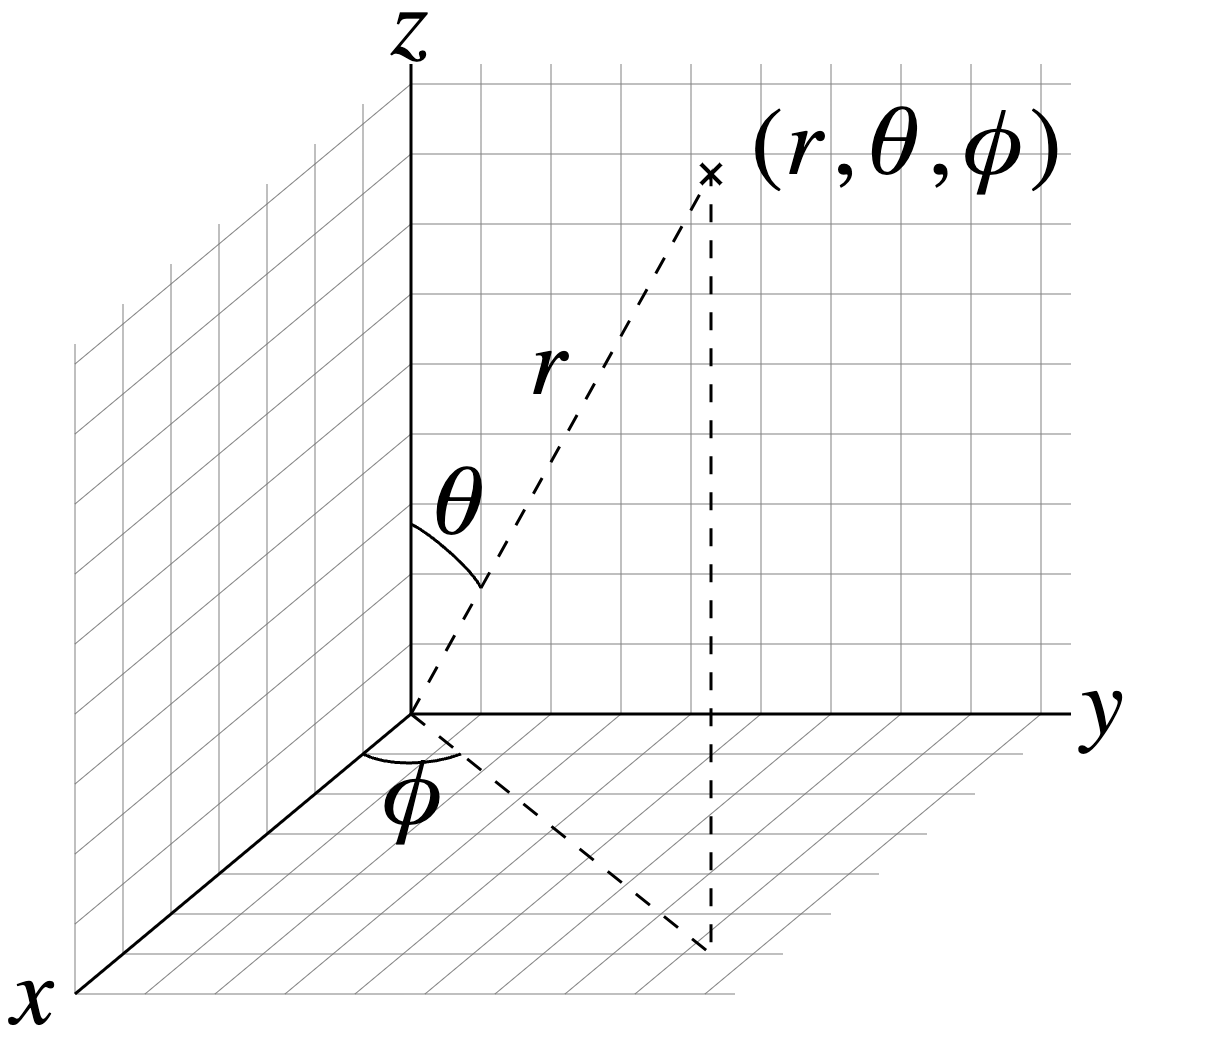
\includegraphics[width=5cm]{../images/spherical_coords_wiki.png}
    \caption{Spherical coordinates from Wikipedia.}
    \label{fig:spherical_coordinates}
\end{figure}

\begin{table}
    \centering
    \begin{tabular} { | Sc | Sc | Sc |}
        \hline
         & total & spectral \\
        \hline
         \begin{tabular}{c} Radiance / \\ Specific intensity \end{tabular} & $ \displaystyle I = \frac{1}{\pi} \sigma T^4 $ & $\displaystyle I_\nu = \frac{2h\nu^3}{c^2} \frac{1}{\exp(h\nu/kT) - 1} $  \\
        \hline
        \begin{tabular}{c} Radiant \\ energy density \end{tabular}  & $\displaystyle E = \frac{4}{c} \sigma T^4 $ & $ \displaystyle E_\nu = \frac{8 \pi h\nu^3}{c^3} \frac{1}{\exp(h\nu/kT) - 1} $ \\
        \hline
        \begin{tabular}{c} One-sided \\ radiant \\ energy flux \end{tabular}  & $\displaystyle S^{\hat{\zvec}} = \sigma T^4 $ & $ \displaystyle S_\nu^{\hat{\zvec}} = \frac{2 \pi h\nu^3}{c^2} \frac{1}{\exp(h\nu/kT) - 1} $ \\
        \hline
    \end{tabular}
    \caption{Radiation quantities for a blackbody spectrum}
    \label{tab:blackbody_quantities}
\end{table}

%%%%%%%%%%%%%%%%%%%%%%%%%%%%%%%%%%%%%%%%%%%%%%%%%%%%%%%%%%%%%%%%%%%%%%%%%
\part{Nuclear Physics}
%%%%%%%%%%%%%%%%%%%%%%%%%%%%%%%%%%%%%%%%%%%%%%%%%%%%%%%%%%%%%%%%%%%%%%%%%

%########################################################################
\chapter{Nuclear Fusion}
%########################################################################

%------------------------------------------------------------------------
\section{Basic definitions}
%------------------------------------------------------------------------
Some basic definitions are provided below:

\begin{itemize}

\item Atomic number ($Z$): \# of protons

\item Mass number ($A$): \# of protons + \# of neutrons

\item Atomic mass ($m_a$): mass of a particular isotope of an element.

\item Relative atomic mass ($A_r$): (defined for an element only)(previously referred to as atomic weight). Average of the atomic masses of all the different isotopes in a \textit{sample}, with each isotope's contribution to the average being its abundance within the sample (as a percentage).

\item Standard Atomic Weight ($A_r^o$): (defined for an element only). Average of the atomic masses of all the different isotopes in \textit{planet earth}, with each isotope's contribution to the average being its abundance in earth (as a percentage).

\item Atomic mass unit ($u$): unit of mass, equivalent to $\frac{1}{12}$ the mass of a carbon-12 atom. That is 
\begin{equation}
\label{eq:def_amu}
1u = \frac{m_c}{12}.
\end{equation}
where $m_c$ is the mass of a carbon-12 atom, in grams. Think of $u$ as similar to a microgram.

\item Mole: \# of elementary entities equal to \# of atoms in 12 grams of carbon-12. That is,
\begin{equation}
1 mol = \frac{12g}{m_c}
\end{equation}
Using \cref{eq:def_amu}, we get
\begin{equation}
\label{eq:u_g_mol}
1u = \frac{1}{mol} g.
\end{equation}
The value of the mole is $6.02214086 \times 10^{23}$.

\item Molar mass ($M$): 
\begin{itemize}
    \item If it is an atom (e.g.\@ Carbon, $C$), then it is its atomic weight, but one uses \cref{eq:u_g_mol} to express the value in $g/mol$. 
    \item If it is a compound (e.g.\@ Methane, $CH_4$), simply add up the atomic weights of each atom in the molecule, and again, express the result in $g/mol$.
    \item If it is a mixture (e.g.\@ air, $N_2,O_2,Ar,CO_2,...$), then it is the weighted average of the atomic weights of the constituents, and the result again is expressed in $g/mol$.
\end{itemize}

\item Avogadro's number ($N_a$): a conversion factor so that things can be measured in terms of moles. 
\begin{equation}
    N_a = \frac{6.02214086 \times 10^{23}}{mol} 
\end{equation}

\end{itemize}
%------------------------------------------------------------------------
\section{The fusion reaction}
%------------------------------------------------------------------------
%--------------------------------------------
\subsection{Energy of a reaction}
%--------------------------------------------
The fundamental relation for nuclear reactions is $E = m c^2$. A mass $m$ can be transformed into energy $E$, and viceversa. Two examples for mass $m$ being transformed into energy are the following:

\begin{itemize}
\item Defect mass: the difference in mass between the atom and the sum of its constituents,
\begin{equation}
m = N m_n + Z m_p - m_a,
\end{equation}
where $m_n$ is the mass of a neutron, $m_p$ the mass of a proton, and $m_a$ the mass of the atom's nucleus. For example, for carbon we have
\begin{equation}
m = 6 \times 1.008664 u + 6 \times 1.007276 u - 12u = 0.09564 u,
\end{equation}
and fluorine
\begin{equation}
m = 10 \times 1.008664 u + 9 \times 1.007276 u - 18.998403u = 0.154 u.
\end{equation}
The binding energy is then the energy corresponding to the mass defect as given by  $E_b = m c^2$.

\item Mass change of a fusion reaction:
\begin{equation}
m = \text{mass of particles before reaction} - \text{mass of particles after reaction} 
\end{equation}
Consider the DT reaction as an example, then we have
\begin{equation}
m = 2.013553u \;(D) + 3.015501u \;(T) - 4.001503u \;(\alpha) - 1.008665u \;(n) = 0.018886u.
\end{equation}
The above mass translates to $E_r = mc^2 = 17.6MeV$.
\end{itemize}

Note that $E_b$ and $E_r$ are related. 
\begin{align}
    E_r &= \left ( \sum_i m_i - \sum_f m_f \right ) c^2 \nonumber \\
    &= \left ( \sum_i m_i - N_i m_{n,i} - Z_i m_{p,i} - \sum_f m_f - N_f m_{n,f} - Z_f m_{p,f}\right ) c^2 \nonumber \\
    &= \sum_f E_{b,f} - \sum_i E_{b,i}.
\end{align}

%--------------------------------------------
\subsection{Energy of reactants}
%--------------------------------------------
As shown in the Material Properties notes, a system of particles colliding with each other can be described by $\rvec_1, \rvec_2, \vvec_1, \vvec_2$. Similarly, this system can be described using the center-of-mass position $\Rvec$, the center-of-mass velocity $\Vvec$, the shifted position $\rvec = \rvec_1 - \rvec_2$ and shifted velocity $\vvec = \vvec_1 - \vvec_2$. Using the shifted velocity, one can define the center-of-mass energy of the initial particles as follows
\begin{equation}
    \epsilon = \frac{1}{2} m_r v^2.
\end{equation}
In the above, $v = |\vvec|$ and $m_r$ is the reduced mass, which satisfies
\begin{equation}
    \frac{1}{m_r} = \frac{1}{m_1} + \frac{1}{m_2}.
\end{equation}

%--------------------------------------------
\subsection{Momentum and energy conservation}
%--------------------------------------------
Lets assume the particles before a fusion reaction move sufficiently slow that their velocities can be neglected, that is, $\epsilon = 0$. Conservation of momentum thus gives
\begin{equation}
0 = m_1 v_1 + m_2 v_2,
\end{equation}
where $m_1$, $m_2$, $v_1$, $v_2$ are the mass and velocity of particles after the reaction.

Energy is not conserved since some of the mass is converted to energy. The energy balance can be written as $E_{after} - E_{before} = E_r$. Assuming again that the particles before a fusion reaction move sufficiently slow, then
\begin{equation}
\frac{1}{2} m_1 v_1^2 + \frac{1}{2} m_2 v_2^2 = E_r,
\end{equation}
where $E_r$ is obtained from Einstein's equation. Combining the last two relations above gives
\begin{align}
    \frac{1}{2} m_1 v_1^2 &= \frac{m_2}{m_1 + m_2} E_r \nonumber \\
    \frac{1}{2} m_2 v_2^2 &= \frac{m_1}{m_1 + m_2} E_r.
\end{align}
That is, the resulting kinetic energy of one of the final particles is proportional to the mass of the other final particle. In other words, the light particle carries most of the energy.

%------------------------------------------------------------------------
\section{Fusion power density}
%------------------------------------------------------------------------
The fusion power density $S_f$ is the fusion energy produced per unit volume per unit time. Label the energy generated by each fusion collision between particles 1 and 2 by $E_f$, and the number of those fusion collisions per unit volume per unit time (also known as reaction rate) as $R_{12}$. Then the fusion power density is given by 
\begin{equation}
    S_f = E_f R_{12}.
\end{equation}
We note that $E_f$ is an energy released by the reaction (it can either be the total energy, the energy carried out by the alpha particles only, the energy carried out by the neutrons only, etc.). 

The reaction rate between two distinct particles is given by
\begin{align}
    R_{12} = n_1 n_2 \langle \sigma v \rangle,
\end{align}
where $n_1$ and $n_2$ are the number densities of particles 1 and 2, respectively. The expected value $\langle \sigma v \rangle$ is given by
\begin{equation}
    \langle \sigma v \rangle = \frac{1}{n_1 n_2} \int_\Rthree \int_\Rthree f_1(\vvec_1) f_2(\vvec_2) \sigma(v) v \, d\vvec_1 d\vvec_2.
\end{equation}
Thus, the fusion power density can be expressed as
\begin{equation}
    S_f = E_f \int_\Rthree \int_\Rthree f_1(\vvec_1) f_2(\vvec_2) \sigma(v) v \, d\vvec_1 d\vvec_2.
\end{equation}
Using the definition of the cross-section, the above can be written as
\begin{equation}
    S_f = E_f \int_\Rthree \int_\Rthree \int_0^{2\pi} \int_0^\infty f_1(\vvec_1) f_2(\vvec_2) F(v,b) v b \, db d\phi d\vvec_1 d\vvec_2.
\end{equation}
For cases in which we are not interested in the energy generated by the collision, but instead on some other physical property associated with the collision (for example change in momentum rather than change in energy) then the above needs to be generalized. Thus, we would use
\begin{equation}
    S = \int_\Rthree \int_\Rthree \int_0^{2\pi} \int_0^\infty f_1(\vvec_1) f_2(\vvec_2) E(v,b) F(v,b) v b \, db d\phi d\vvec_1 d\vvec_2,
\end{equation}
where $E(v,b)$ is the physical property associated with the collision.

%%%%%%%%%%%%%%%%%%%%%%%%%%%%%%%%%%%%%%%%%%%%%%%%%%%%%%%%%%%%%%%%%%%%%%%%%
\part{Atomic Physics}
%%%%%%%%%%%%%%%%%%%%%%%%%%%%%%%%%%%%%%%%%%%%%%%%%%%%%%%%%%%%%%%%%%%%%%%%%

%########################################################################
\chapter{Equation of state}
%########################################################################

%########################################################################
\chapter{Opacities}
%########################################################################
There are multiple processes that control the behavior of photons:
\begin{itemize}
    \item Absorption 
    \begin{itemize}
        \item Bound-bound excitation (\textbf{stimulated absorption})
        \item Bound-free ionization (\textbf{photoionization})
        \item Free-free photo-absorption (\textbf{inverse breemstrahlung})
    \end{itemize}
    \item Emission 
    \begin{itemize}
        \item Bound-bound de-excitation (\textbf{stimulated emission}, \textbf{spontaneous emission})
        \item Free-bound recombination
        \item Free-free photo-emission (\textbf{breemstrahlung})
    \end{itemize}
    \item Scattering
    \begin{itemize}
        \item \textbf{Rayleigh scattering}: elastic scattering of a photon from an atom or molecule whose size is less than that of the wavelength of the photon. 
        \item \textbf{Mie scattering}: same as Rayleigh scattering but for cases where the sizes of the atoms or molecules are comparable to the wavelength of the incoming photon.
        \item \textbf{Raman scattering}: inelastic scattering of a photon from a molecule. The interaction changes the molecule's vibrational, rotational, or electron energy.
        \item \textbf{Brillouin scattering}: inelastic scattering of a photon caused by its interaction with material waves in a medium (i.e. mass oscillation modes, charge displacement modes, magnetic spin oscillation modes). 
        \item \textbf{Compton scattering}: inelastic scattering of a photon from a charged particle. 
        \item \textbf{Thomson scattering}: low-energy limit of Compton scattering. The photon energy and the particle's kinetic energy do not change as a result of the scattering. Can be explained with classical electrodynamics.
    \end{itemize}
    \item Reflection
    \item Transmission (nothing happens)
    \item \textbf{Pair production/annihilation}
\end{itemize}

Each of the above would alter the beam of photons passing through the material (except for transmission). The cross-sections of each process, which would depend on the incoming photon frequency $\nu$, can be added up to obtain a total cross section $\sigma = \sigma(\nu)$. From the definition of a cross section, $\sigma$ can be used to determine how many photons keep their course as they traverse through the material and how many do not. Consider the material under consideration to have the shape of a thick slab, which starts at $x=0$ and continues on for a definite length along $x>0$. We want to know how $I(x)$, the number of photons crossing the slab at any location $x$, decreases as we travel along the $x$ direction. Let's focus on an infinitesimal thin lamina within the slab, of width $dx$ and located at some arbitrary location $x$. The number of target particles in that lamina will be $n dx$, where $n$ is the number volume density of particles in the target material. Then, the number of incident photons after crossing the lamina would be
\begin{equation}
    I(x+dx) = I(x) -\sigma I(x) n dx.
\end{equation}
This leads to the ODE $dI(x)/dx = -\sigma I(x) n$, which has as solution
\begin{equation}
    I(x) = I(0) \exp(-\sigma n x).
\end{equation}
The attenuation coefficient is defined as $\sigma n$ [1/cm]. The mass attenuation coefficient, also referred to as opacity, is then given by $\kappa = \sigma n / \rho$ [cm\textsuperscript{2}/g]. $\Lambda = 1 / \sigma n$ is referred to as the attenuation length. 

%%%%%%%%%%%%%%%%%%%%%%%%%%%%%%%%%%%%%%%%%%%%%%%%%%%%%%%%%%%%%%%%%%%%%%%%%
\part{Laser Physics}
%%%%%%%%%%%%%%%%%%%%%%%%%%%%%%%%%%%%%%%%%%%%%%%%%%%%%%%%%%%%%%%%%%%%%%%%%

%########################################################################
\chapter{Some notes on lasers}
%########################################################################
Consider a wave that depends on time $t$ and single spatial dimension $x$, which is orthogonal to the direction of propagation. 

A wave is spatially coherent at a given time $t$, position $x$, and separation distance $L$ if the phase difference between the points $x$ and $x+L$ at time $t$ is the same as that at a later time $t+dt$. You can keep on picking larger and larger values of $L$ until this is not the case, this $L$ would be the spatial coherence length $L_c$ = $L_c(t,x)$.

A wave is temporally coherent at a given time $t$, position $x$, and separation time $\tau$ if the phase difference between times $t$ and $t+\tau$ at position $x$ is the same as that between times $t+dt$ and $t+dt+\tau$. You can keep on picking larger and larger values of $\tau$ until this is no longer the case, this $\tau$ would be the temporal coherence length $\tau_c = \tau_c(t,x)$.

\begin{figure}
    \centering
    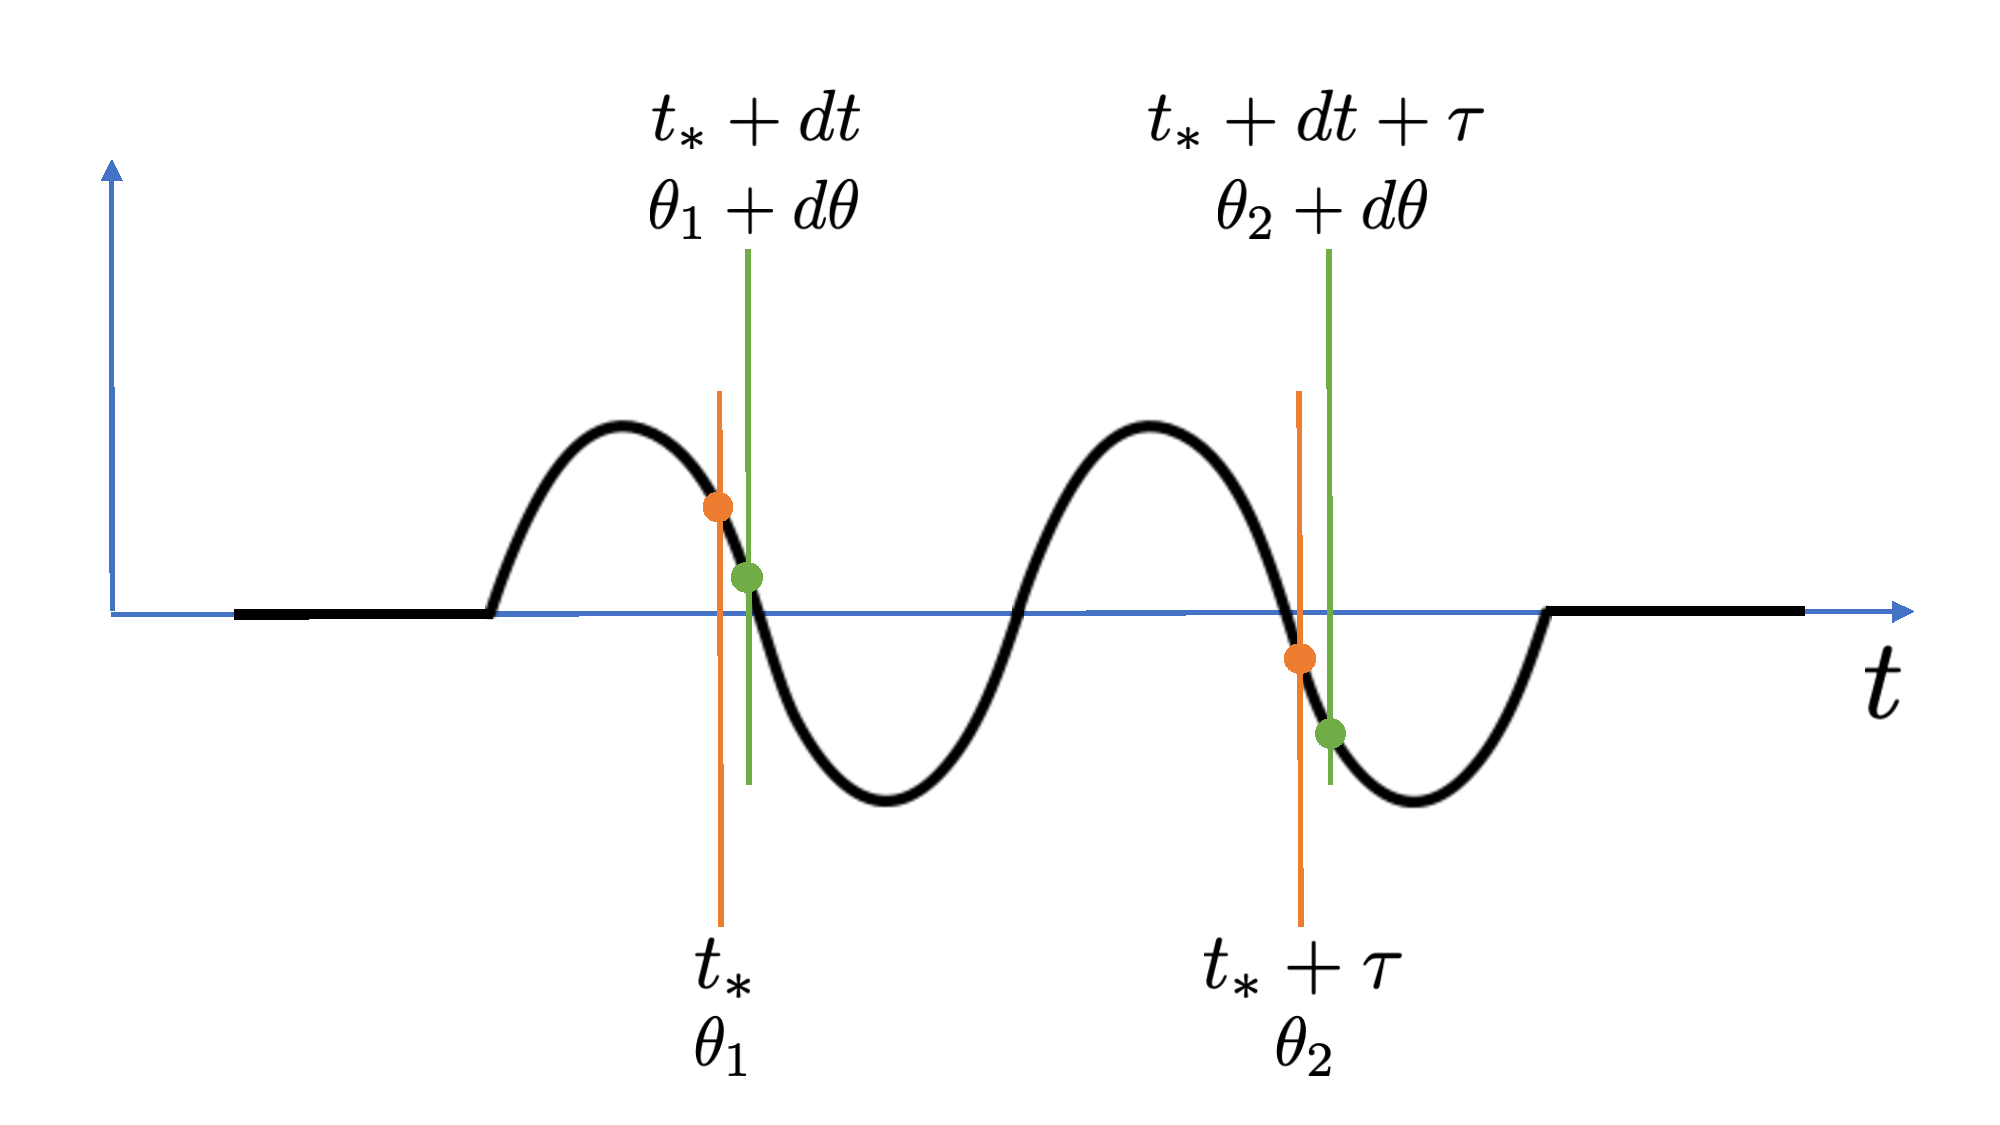
\includegraphics[width=.7\textwidth]{../images/temp_cohe_1.pdf}
    \caption{}
    \label{fig:laser_temp_cohe}
\end{figure}

\begin{figure}
    \centering
    \begin{subfigure}{.7\textwidth}
      \centering
      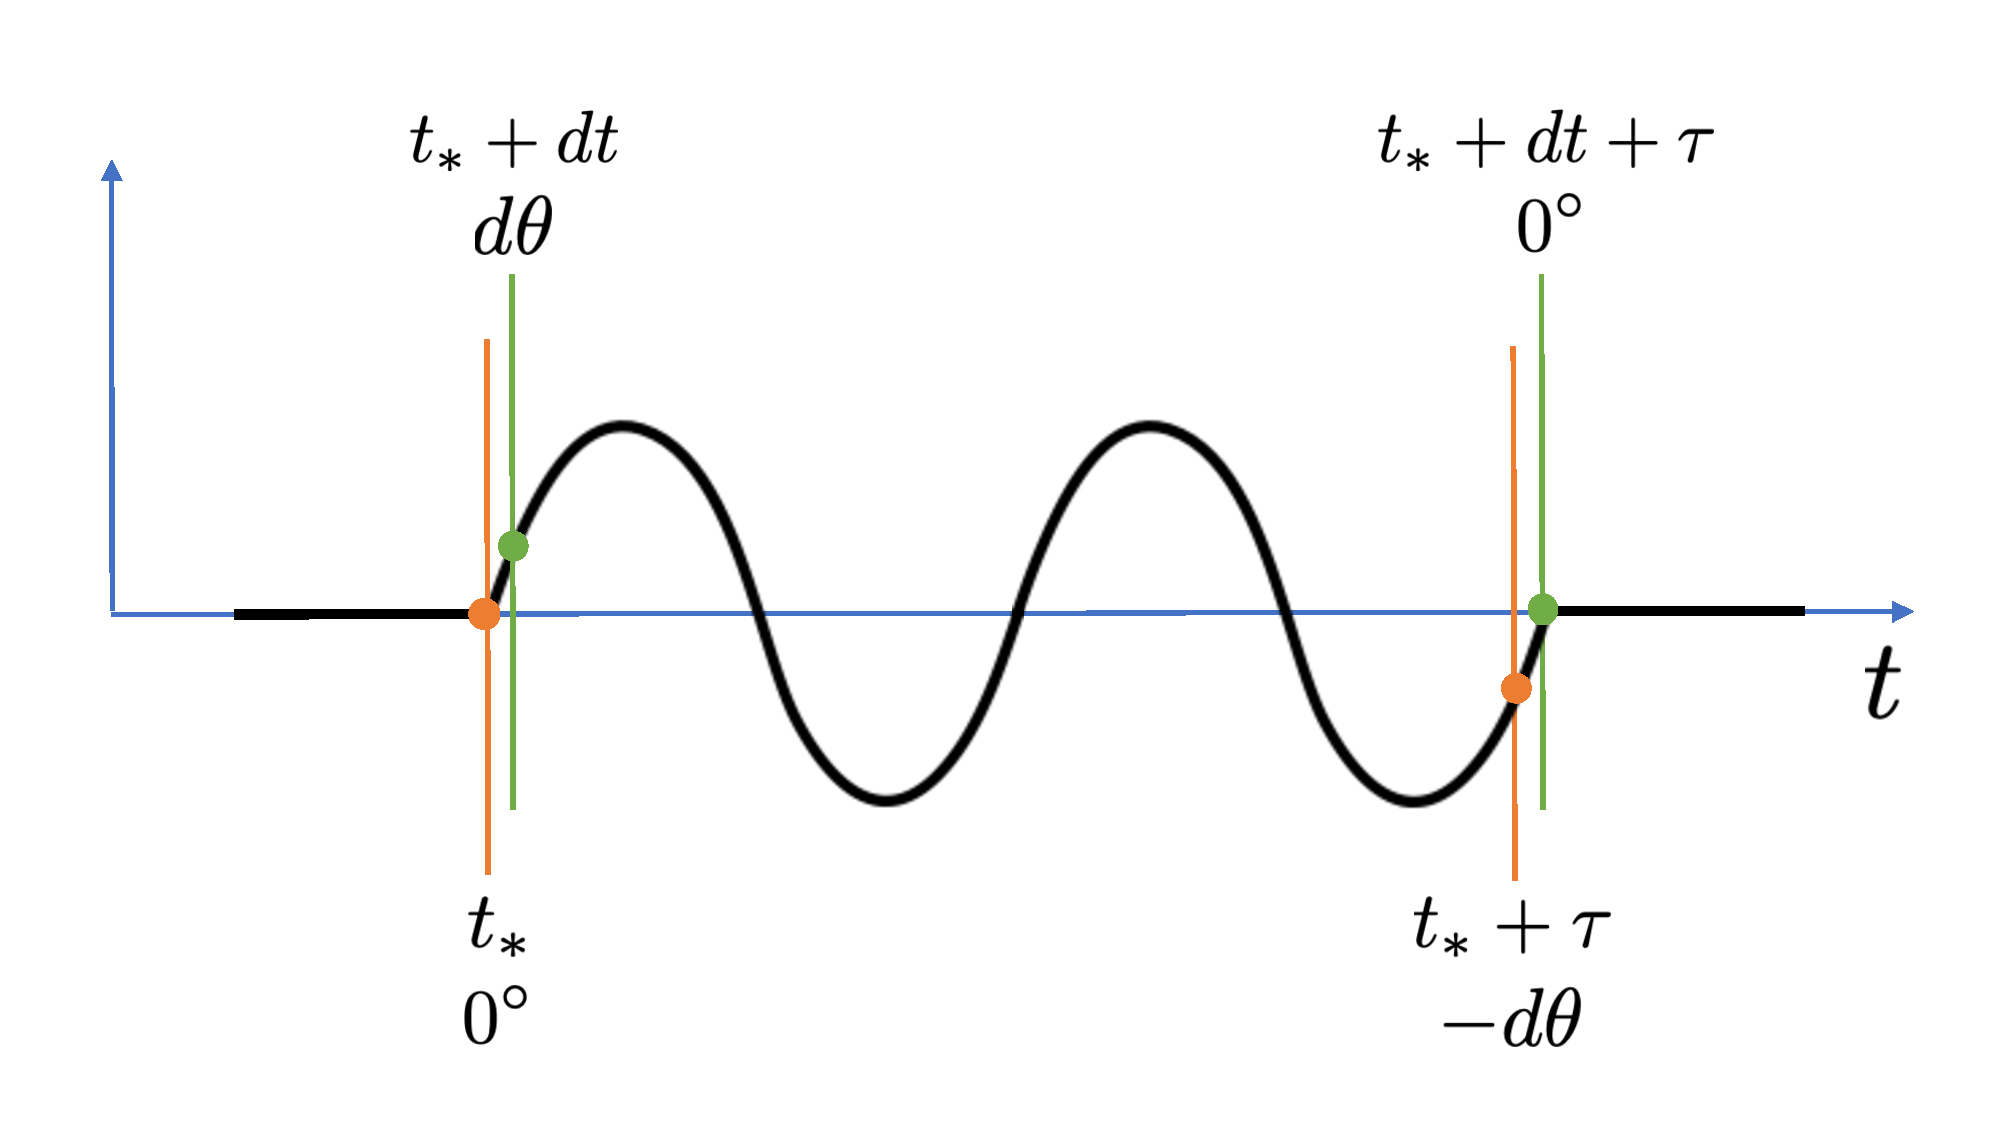
\includegraphics[width=\textwidth]{../images/temp_cohe_2.pdf}
      \caption{}
      \label{fig:laser_temp_cohe_1}
    \end{subfigure}
    \begin{subfigure}{.7\textwidth}
        \centering
        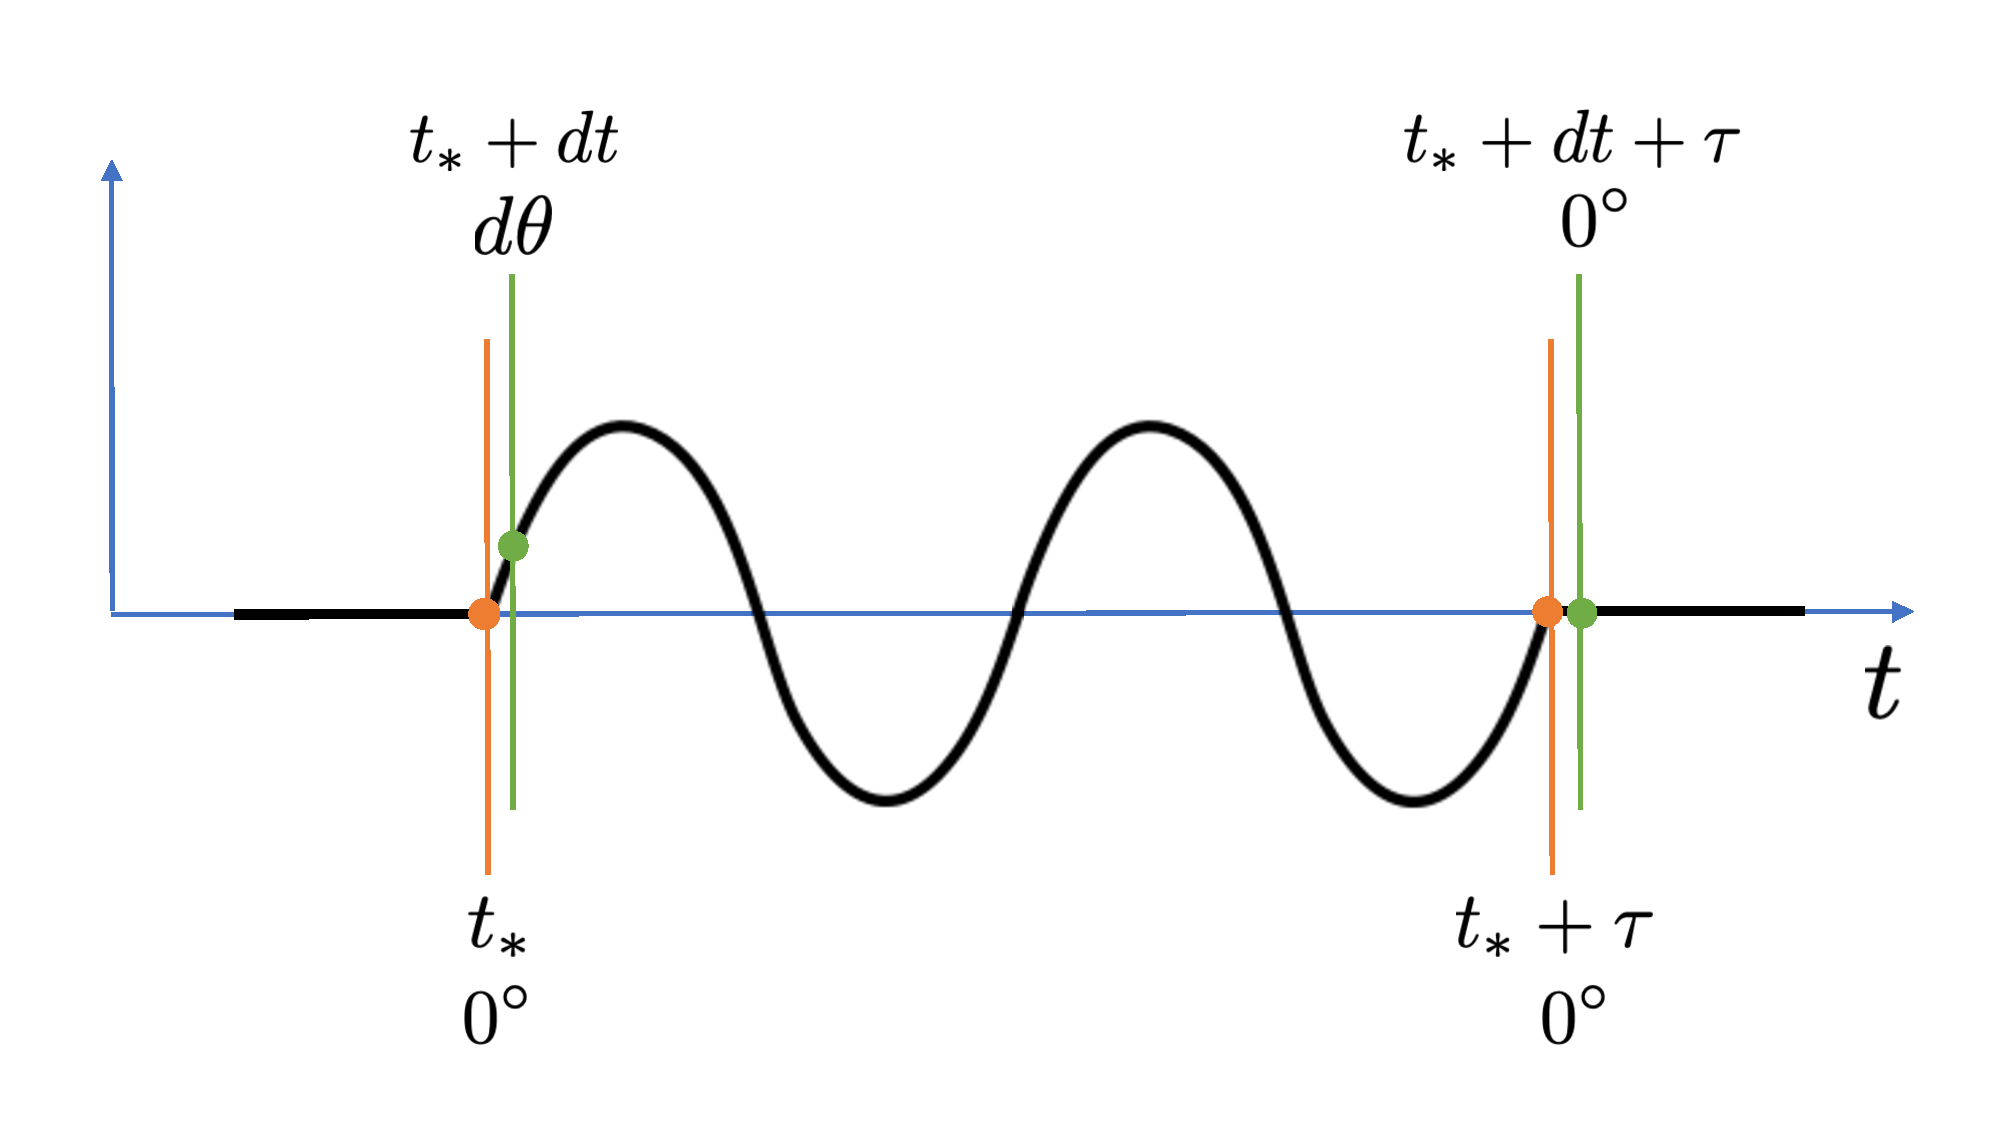
\includegraphics[width=\textwidth]{../images/temp_cohe_3.pdf}
        \caption{}
        \label{fig:laser_temp_cohe_2}
      \end{subfigure}
    \caption{Depiction of temporal coherence for a light pulse.}
    \label{fig:laser_temp_cohe_12}
\end{figure}

A depiction of temporal coherence is provided in \cref{fig:laser_temp_cohe}, which shows a light pulse as a function of time. An arbitrary time $t_*$ is chosen along the light wave, and the wave's phase at that time is $\theta_1$. At the time $t_* + \tau$ the wave has a different phase $\theta_2$, and thus the phase difference between times $t_*$ and $t_*+\tau$ is $\theta_2 - \theta_1$. This is depicted by the orange dots. The green dots are used to highlight the phase difference between times $t_*+dt$ and $t_*+dt+\tau$. In this case, the phases are respectively $\theta_1 + d\theta$ and $\theta_2 + d\theta$, and hence the phase difference is still maintained at $\theta_2 - \theta_1$.

Rather than picking the time $t_*$ to be at an arbitrary location along the wave, in \cref{fig:laser_temp_cohe_1} we choose $t_*$ to be at the beginning of the wave, and also choose $\tau$ to be just a bit smaller than the entire duration of the pulse. For this case, the phase difference between $t_*$ and $t_*+\tau$ is $d\theta$, which is equal to the phase difference between $t_*+dt$ and $t_*+dt+\tau$. On the other hand, in \cref{fig:laser_temp_cohe_2} we have chosen $\tau$ to be just a bit larger so as to be equal to the duration of the wave. For this case the phase difference between $t_*$ and $t_*+\tau$ is zero, which is not the same as the phase difference between $t_*+dt$ and $t_*+dt+\tau$, namely $d\theta$. Thus, the maximum value of $\tau$ that maintains a constant phase difference has been reached, and therefore by definition this value is referred to as the temporal coherence length $\tau_c$ at time $t_*$ (other locations of $t_*$, such as that in \cref{fig:laser_temp_cohe}, have a different $\tau_c$).

%########################################################################
\chapter{Longitudinal and transverse waves}
%########################################################################

%------------------------------------------------------------------------
\section{Definitions}
%------------------------------------------------------------------------
The Helmholtz decomposition for a function $\Fvec = \Fvec(\xvec,t)$ is of the following form
\begin{equation}
    \Fvec = \Fvec_l + \Fvec_t,
\end{equation}
where $\Fvec_l = \Fvec_l(\xvec,t)$ is the longitudinal component and $\Fvec_t = \Fvec_t(\xvec,t)$ the transverse component. These are defined by
\begin{align}
    \nabla \times \Fvec_l &= 0, \label{eq:ltw_plasma_long_def}\\
    \nabla \cdot \Fvec_t &= 0. \label{eq:ltw_plasma_tran_def}
\end{align}
We'll assume that any vector function $\Gvec = \Gvec(\xvec,t)$ can be expressed as the real component of
\begin{equation}
    \label{eq:em_more_general_wave_form}
    \Gvec = \hat{\Gvec} \exp \left [ i \left ( \int_0^x k_x(x') \, dx' + \int_0^y k_y(y') \, dy' + \int_0^z k_z(z') \, dz'  - wt \right ) \right ].
\end{equation}
For the above, $w$ a frequency constant in time and space, and $k_x = k_x(x)$, $k_y = k_y(y)$, and $k_z = k_z(z)$ form the wave vector $\kvec = [k_x, k_y, k_z]$. $\hat{\Gvec} = \hat{\Gvec}(\xvec,t)$ is a complex vector where the real and complex components point in the same direction. Additionally, we enforce the constraint that if $\nabla \times \Gvec = 0$, then $\nabla \times \hat{\Gvec} = 0$, and similarly, if $\nabla \cdot \Gvec = 0$, then $\nabla \cdot \hat{\Gvec} = 0$. We'll often use a different subscript in the wave vectors and frequencies of different waves. For example, we'll use $\kvec_e$ for electron-plasma waves, $\kvec_i$ for ion-acoustic waves, $\kvec_L$ for laser waves, and $\kvec_s$ for scattered waves. Similarly for the frequencies $w_e$, $w_i$, $w_L$, $w_s$.

We note that
\begin{multline}
    \nabla \exp \left [ i \left ( \int_0^x k_x(x') \, dx' + \int_0^y k_y(y') \, dy' + \int_0^z k_z(z') \, dz'  - wt \right ) \right ] \\
    = i \kvec \exp \left [ i \left ( \int_0^x k_x(x') \, dx' + \int_0^y k_y(y') \, dy' + \int_0^z k_z(z') \, dz'  - wt \right ) \right ]
\end{multline}
Given the identity $\nabla \times (\Avec f) = (\nabla \times \Avec ) f - \Avec \times (\nabla f)$, we can show that
\begin{align}
    \label{eq:ltw_no_curl}
    \nabla \times \Gvec &= \nabla \times \left [ \hat{\Gvec} \exp (...) \right ] \nonumber \\
    &= \left ( \nabla \times \hat{\Gvec} \right ) \exp (...) - \hat{\Gvec} \times \left [ \nabla \exp (...) \right ] \nonumber \\
    &= \left ( \nabla \times \hat{\Gvec} \right ) \exp (...) - \hat{\Gvec} \times \left [ i\kvec \exp (...) \right ] \nonumber \\
    &= \left ( \nabla \times \hat{\Gvec} \right ) \exp (...) + i \kvec \times \Gvec.
\end{align}
Given the identity $\nabla \cdot (\Avec f) = ( \nabla \cdot \Avec) f + \Avec \cdot (\nabla f)$, we can show that
\begin{align}
    \label{eq:ltw_no_div}
    \nabla \cdot \Gvec &= \nabla \cdot \left [ \hat{\Gvec} \exp (...) \right ] \nonumber \\
    &= \left ( \nabla \cdot \hat{\Gvec} \right ) \exp (...) + \hat{\Gvec} \cdot \left [ \nabla \exp (...) \right ] \nonumber \\
    &= \left ( \nabla \cdot \hat{\Gvec} \right ) \exp (...) + \hat{\Gvec} \cdot \left [ i \kvec \exp (...) \right ] \nonumber \\
    &= \left ( \nabla \cdot \hat{\Gvec} \right ) \exp (...) + i \kvec \cdot \Gvec.
\end{align}
By definition, $\Fvec_l$ has no curl and $\Fvec_t$ has no divergence. As mentioned earlier, we then require $\hat{\Fvec}_l$ to have no curl and $\hat{\Fvec}_t$ to have no divergence. Using this in \cref{eq:ltw_no_curl,eq:ltw_no_div} allow us to write
\begin{align}
    \kvec \times \Fvec_l = 0 \label{eq:ltw_plasma_long_wavevector} \\
    \kvec \cdot \Fvec_t = 0 \label{eq:ltw_plasma_trans_wavevector}.
\end{align}

The first expression above says $\Fvec_l$ is parallel to $\kvec$ and the second says $\Fvec_t$ is orthogonal to $\kvec$. Thus, $\Fvec_l \cdot \Fvec_t = 0$. We will often have situations where $\nabla \times \Fvec = \nabla \cdot \Fvec = 0$, which by its own does not imply $\Fvec = 0$. However, using \cref{eq:ltw_no_curl,eq:ltw_no_div}, this translates to to $\kvec \times \Fvec = \kvec \cdot \Fvec =  0$. The latter equality states that $\kvec$ and $\Fvec$ are orthogonal, that is, the angle between them is $90^\circ$. The former equality leads to $|\Fvec| \sin(90^\circ) = 0$, which in turn means $\Fvec = 0$. To summarize,
\begin{equation}
    \label{eq:ltw_general_null_vector}
    \nabla \times \Fvec = \nabla \cdot \Fvec = 0 \to \Fvec = 0.
\end{equation}

For some cases we'll further restrict $\hat{\Gvec}$ in \cref{eq:em_more_general_wave_form} such that $\hat{\Gvec} = \hat{\Gvec} (\xvec)$, that is, the time dependence of the wave is fully captured by the $\exp(-iwt)$ term. For this case, we'll often re-write the expression for $\Gvec$ as
\begin{equation}
    \label{eq:em_semi_general_wave_form}
    \Gvec = \tilde{\Gvec} \exp (-iwt),
\end{equation}
where $\tilde{\Gvec} = \tilde{\Gvec}(\xvec)$ is given by
\begin{equation}
    \tilde{\Gvec} = \hat{\Gvec} \exp \left [ i \left ( \int_0^x k_x(x') \, dx' + \int_0^y k_y(y') \, dy' + \int_0^z k_z(z') \, dz' \right ) \right ].
\end{equation}
Finally, a further simplification occurs when $\kvec$ and $\hat{\Gvec}$ are assumed to be constant in space. For this case, the expression for $\Gvec$ becomes
\begin{equation}
    \label{eq:em_general_wave_form}
    \Gvec = \hat{\Gvec} \exp \left [i\left ( \kvec \cdot \xvec - wt \right ) \right ].
\end{equation}
These are the so-called plane waves. We end with the cautionary note that the second gradients of $\Gvec$ in \cref{eq:em_more_general_wave_form} are not necessarily the same as those of $\Gvec$ in \cref{eq:em_general_wave_form}.

%------------------------------------------------------------------------
\section{Electron-plasma and ion-acoustic waves}
%------------------------------------------------------------------------
For both electron-plasma and ion-acoustic waves we can assume the magnetic field does not change. Thus, Faraday's law gives
\begin{equation}
    \nabla \times \Evec = \nabla \times \Evec_t = 0.
\end{equation}
By definition, $\nabla \cdot \Evec_t = 0$. Thus, using \cref{eq:ltw_general_null_vector} we get $\Evec_t = 0$, that is, $\Evec = \Evec_l$. 

For electron-plasma waves, we can use \cref{eq:em_general_wave_form} to write \cref{eq:ep_waves_mom_linearized} in spectral form and thus obtain
\begin{equation}
-i w n_{e0} \hat{\uvec}_{e1} + \frac{e n_{e0}}{m_e} \hat{\Evec}_{1,l} = -\kvec_e \frac{\gamma_e p_{e0}}{n_{e0} m_e} \hat{n}_{e1}. 
\end{equation}
Since the second term on the left-hand side and the term on the right-hand side point along $\kvec_e$, $\hat{\uvec}_{e1}$ also points along $\kvec_e$, that is, $\hat{\uvec}_{e1} = \hat{\uvec}_{e1,l}$.

For ion-acoustic waves, we can use \cref{eq:em_general_wave_form} to write \cref{eq:ia_waves_mom_linearized} in spectral form and thus obtain
\begin{equation}
-i w n_{i0} \hat{\uvec}_{i1} - \frac{Z e n_{i0}}{m_i} \hat{\Evec}_{1,l} = -\kvec_i \frac{\gamma_i p_{i0}}{n_{i0} m_i} \hat{n}_{i1}. 
\end{equation}
Since the second term on the left-hand side and the term on the right-hand side point along $\kvec_i$, $\hat{\uvec}_{i1}$ also points along $\kvec_i$, that is, $\hat{\uvec}_{i1} = \hat{\uvec}_{i1,l}$. Finally, we note that the electric field being purely longitudinal is in agreement with \cref{eq:ia_waves_E}.

%########################################################################
\chapter{Electromagnetic waves in plasmas}
%########################################################################

\label{sec:electromagnetic_waves_plasmas}
In introductory electrodynamics, one typically studies electromagnetic waves in vacuum, that is, for cases where $\rho_e = \Jvec = 0$. In this section we relax both of these assumptions. Consider the electric and magnetic fields as well as the scalar and vector potentials, which satisfy
\begin{equation}
    \label{eq:emp_general_E_potential}
    \Evec = -\nabla \phi - \frac{\partial \Avec}{\partial t},
\end{equation}
\begin{equation}
    \label{eq:emp_general_B_potential}
    \Bvec = \nabla \times \Avec.
\end{equation}
For the above, we choose $\nabla \cdot \Avec = 0$. Using the fact that the magnetic field is solenoidal, we have
\begin{equation*}
    \nabla \cdot \Bvec = \nabla \cdot \Bvec_l + \nabla \cdot \Bvec_t = \nabla \cdot \Bvec_l = 0.
\end{equation*}
However, by definition, $\nabla \times \Bvec_l = 0$ as well. Thus, using \cref{eq:ltw_general_null_vector}, we have $\Bvec_l = 0$. The same argument applies to the vector potential, and thus $\Avec_l = 0$. For the electric field, we have
\begin{equation*}
    \nabla \cdot \Evec = \nabla \cdot \Evec_l + \nabla \cdot \Evec_t = \nabla \cdot \Evec_l .
\end{equation*}
Taking the divergence of \cref{eq:emp_general_E_potential}, we get
\begin{equation}
    \nabla \cdot \Evec = \nabla \cdot \left ( -\nabla \phi \right ).
\end{equation}
Combining the last two equations gives
\begin{equation*}
    \nabla \cdot \left ( \Evec_l + \nabla \phi \right ) = 0.
\end{equation*}
By definition, we also have
\begin{equation*}
    \nabla \times \left ( \Evec_l + \nabla \phi \right ) = 0.
\end{equation*}
Thus, using \cref{eq:ltw_general_null_vector}, we have $\Evec_l = -\nabla \phi$. A similar argument can be used to show $\Evec_t = -\partial \Avec / \partial t$. Our goal in this section will be to determine equations for $\Evec_l$, $\Evec_t$ and $\Bvec$.

We'll begin with the conservation of charge equation
\begin{equation*}
    \frac{\partial \rho_e}{\partial t} + \nabla \cdot \Jvec = 0,
\end{equation*}
which we re-write as
\begin{equation*}
    \frac{\partial \rho_e}{\partial t} + \nabla \cdot \Jvec_l = 0,
\end{equation*}
Using Poisson's equation $\nabla^2\phi = -\rho_e / \epsilon_0$ in the above, we get
\begin{equation*}
    \frac{\partial}{\partial t} \left ( -\epsilon_0 \nabla^2 \phi \right ) + \nabla \cdot \Jvec_l = 0,
\end{equation*}
or
\begin{equation*}
    \nabla \cdot \left ( \frac{\partial \nabla \phi}{\partial t} - \frac{1}{\epsilon_0} \Jvec_l \right ) = 0.
\end{equation*}
However, by definition, we also have
\begin{equation*}
    \nabla \times \left ( \frac{\partial \nabla \phi}{\partial t} - \frac{1}{\epsilon_0} \Jvec_l \right ) = 0.
\end{equation*}
Using \cref{eq:ltw_general_null_vector}, we conclude
\begin{equation}
    \label{eq:emp_general_longitudinal_J}
    \frac{\partial \nabla \phi}{\partial t} = \frac{1}{\epsilon_0} \Jvec_l.
\end{equation}
This gives the equation for $\Evec_l$, namely,
\begin{equation}
    \label{eq:emp_general_long_E}
    \frac{\partial^2 \Evec_l}{\partial t^2} + \frac{1}{\epsilon_0} \frac{\partial \Jvec_l}{\partial t} = 0.
\end{equation}

Both $\Evec_t$ and $\Bvec$ can be extracted from $\Avec$, so now we proceed to find an equation for the transverse vector potential. Ampere's law with Maxwell's correction gives
\begin{equation*}
    \nabla \times \left ( \nabla \times \Avec \right ) = \mu_0 \Jvec + \mu_0 \epsilon_0 \frac{\partial \Evec}{\partial t}.
\end{equation*}
The above is re-written as
\begin{equation*}
    \nabla \left ( \nabla \cdot \Avec \right ) - \nabla^2 \Avec = \mu_0 \Jvec + \mu_0 \epsilon_0 \left ( -\frac{\partial \nabla \phi}{\partial t} - \frac{\partial^2 \Avec}{\partial t^2} \right ),
\end{equation*}
which gives
\begin{equation*}
    \frac{\partial^2 \Avec}{\partial t} - \frac{1}{\mu_0 \epsilon_0} \nabla^2 \Avec = \frac{1}{\epsilon_0} \Jvec - \frac{\partial \nabla \phi}{\partial t},
\end{equation*}
or
\begin{equation*}
    \frac{\partial^2 \Avec}{\partial t} - c_0^2 \nabla^2 \Avec = \frac{1}{\epsilon_0} \Jvec - \frac{\partial \nabla \phi}{\partial t},
\end{equation*}
where $c_0 = 1/\sqrt{\mu_0 \epsilon_0}$. Expanding the current density as $\Jvec = \Jvec_l + \Jvec_t$, and using \cref{eq:emp_general_longitudinal_J}, we get
\begin{equation}
    \label{eq:emp_general_trans_vec_pot}
    \frac{\partial^2 \Avec}{\partial t} - c_0^2 \nabla^2 \Avec = \frac{1}{\epsilon_0} \Jvec_t.
\end{equation}
Using the functional form in \cref{eq:em_general_wave_form} for $\Avec$ and $\Jvec_t$ gives
\begin{equation}
    -w^2 \hat{\Avec} + k^2 c_0^2 \hat{\Avec}= \frac{1}{\epsilon_0} \hat{\Jvec}_t.
\end{equation}
That is, $\Avec$ and $\Jvec_t$ point in the same direction.

Taking the time derivative of \cref{eq:emp_general_trans_vec_pot} gives the equation for $\Evec_t$, that is
\begin{equation}
    \label{eq:emp_general_trans_E}
    \frac{\partial^2 \Evec_t}{\partial t^2} - c_0^2 \nabla^2 \Evec_t + \frac{1}{\epsilon_0} \frac{\partial \Jvec_t}{\partial t} = 0.
\end{equation}
Taking the curl of \cref{eq:emp_general_trans_vec_pot} gives the equation for $\Bvec$, that is
\begin{equation}
    \label{eq:emp_general_trans_B}
    \frac{\partial^2 \Bvec}{\partial t^2} - c_0^2 \nabla^2 \Bvec - \frac{1}{\epsilon_0} \nabla \times \Jvec_t = 0.
\end{equation}
Using the functional form in \cref{eq:em_general_wave_form} for $\Evec_t$, $\Bvec$ and $\Jvec_t$ gives
\begin{equation}
    -w^2 \hat{\Evec}_t + k^2 c_0^2 \hat{\Evec}_t - \frac{iw}{\epsilon_0} \hat{\Jvec}_t = 0,
\end{equation}
\begin{equation}
    -w^2 \Bvec + k^2 c_0^2 \Bvec - \frac{i}{\epsilon_0} \kvec \times \Jvec_t = 0.
\end{equation}
That is, $\Evec_t$ points in the same direction as $\Jvec_t$, which as shown before points in the same direction as $\Avec$. Additionally, $\Bvec$ points in the direction of $\kvec \times \Jvec_t$, that is, it is orthogonal to $\Evec_t$.

We briefly note that taking the curl of \cref{eq:p_waves_maxwell_1}, and using \cref{eq:p_waves_maxwell_2}, gives the wave equation for the total electric field $\Evec$, that is 
\begin{equation}
    \frac{\partial^2 \Evec}{\partial t^2} - c_0^2 \nabla^2 \Evec + c_0^2 \nabla (\nabla \cdot \Evec) + \frac{1}{\epsilon_0} \frac{\partial \Jvec}{\partial t} = 0.
\end{equation}
The above can be considered as the sum of the following three equations
\begin{align*}
    \frac{\partial^2 \Evec_l}{\partial t^2} + \frac{1}{\epsilon_0} \frac{\partial \Jvec_l}{\partial t} &= 0, \\
    \frac{\partial^2 \Evec_t}{\partial t^2} - c_0^2 \nabla^2 \Evec_t + \frac{1}{\epsilon_0} \frac{\partial \Jvec_t}{\partial t} &= 0, \\
    -c_0^2 \nabla^2 \Evec_l + c_0^2 \nabla (\nabla \cdot \Evec_l) &= 0.
\end{align*}
The first is the equation for the longitudinal electric field, that is \cref{eq:emp_general_long_E}. The second is the equation for the transverse electric field, that is \cref{eq:emp_general_trans_E}. The third equation above follows from the vector identity $\nabla \times (\nabla \times \Fvec) = -\nabla^2 \Fvec + \nabla ( \nabla \cdot \Fvec )$ and the fact that $\nabla \times \Evec_l = 0$.

It will often be the case that transverse waves will oscillate at such a fast rate that the ions, which have a large inertia, will be unable to react quickly enough. Thus, we can assume $\uvec_{i,t} = 0$. Given the definition of the current density in \cref{eq:p_waves_curr_density}, the transverse current density is expressed as $\Jvec_t = e \left (Z n_i \uvec_{i,t} - n_e \uvec_{e,t} \right )$, which now simplifies to 
\begin{equation}
    \label{eq:emp_transverse_current}
    \Jvec_t = -e n_e \uvec_{e,t}.
\end{equation}
Thus, the transverse electron velocity $\uvec_{e,t}$ points in the same direction as $\Jvec_t$, which is the same direction as $\Evec_t$ and $\Avec$. The next section focuses on deriving an expression for $\uvec_{e,t}$. 

We begin with \cref{eq:pwaves_electron_momentum}, the electron momentum equation, which, due to the electron continuity equation, can be written as
\begin{equation*}
    m_e n_e \frac{\partial\uvec_e}{\partial t} + m_e n_e \uvec_e \cdot \nabla \uvec_e + e n_e \left ( \Evec + \uvec_e \times \Bvec \right ) = -\nabla p_e,
\end{equation*}
or
\begin{equation*}
    \frac{\partial\uvec_e}{\partial t} + \uvec_e \cdot \nabla \uvec_e + \frac{e}{m_e} \left ( \Evec + \uvec_e \times \Bvec \right ) = -\frac{1}{n_e m_e}\nabla p_e,
\end{equation*}
Using the scalar and vector potentials we have
\begin{equation*}
    \frac{\partial\uvec_e}{\partial t} + \uvec_e \cdot \nabla \uvec_e +\frac{e}{m_e} \left [ -\nabla \phi - \frac{\partial \Avec}{\partial t} + \uvec_e \times \left ( \nabla \times \Avec \right ) \right ] = -\frac{1}{n_e m_e} \nabla p_e.
\end{equation*}
Using the vector identity $\nabla \left ( F^2 / 2 \right ) = \Fvec \times \left ( \nabla \times \Fvec \right ) + \Fvec \cdot \nabla \Fvec$, we write the above as
\begin{equation}
    \frac{\partial\uvec_e}{\partial t} - \uvec_e \times \left ( \nabla \times \uvec_e \right ) + \nabla \left (\frac{u_e^2}{2} \right ) + \frac{e}{m_e} \left [ -\nabla \phi - \frac{\partial \Avec}{\partial t} + \uvec_e \times \left ( \nabla \times \Avec \right ) \right ] = -\frac{1}{n_e m_e} \nabla p_e,
\end{equation}
which is equivalent to 
\begin{equation}
    \label{eq:emp_electron_momentum}
    \frac{\partial\uvec_e}{\partial t} - \uvec_e \times \left ( \nabla \times \uvec_{e,t} \right ) + \nabla \left (\frac{u_e^2}{2} \right ) + \frac{e}{m_e} \left [ -\nabla \phi - \frac{\partial \Avec}{\partial t} + \uvec_e \times \left ( \nabla \times \Avec \right ) \right ] = -\frac{1}{n_e m_e} \nabla p_e.
\end{equation}
We'll now introduce a more specific coordinate system. We'll be dealing with at most three waves at a time: a laser wave, a scattered wave, and a plasma wave (either electron-plasma or ion-acoustic wave). We'll assume all three of these waves lie on a so-called base plane. That is, $\kvec_e$ (or $\kvec_i$), $\kvec_L$, and $\kvec_s$ all point along this plane. We now choose the main transverse direction, that is, the direction of $\uvec_{e,t}$, $\Jvec_t$, $\Evec_t$, and $\Avec$ to be the direction orthogonal to this plane, so that these vectors are orthogonal to any $\kvec$. As an aside, we note that the longitudinal and transverse components of the electron velocity can belong to different waves. That is
\begin{align}
    \uvec_{e,l} &= \hat{\uvec}_{e,l} \exp \left [ i (\kvec_p \cdot \xvec - w_pt) \right ] \\
    \uvec_{e,t} &= \hat{\uvec}_{e,t} \exp \left [ i (\kvec_q \cdot \xvec - w_qt) \right ].
\end{align}
The vectors $\nabla \left ( u_e^2 / 2 \right )$, $\nabla \phi$ and $\nabla p_e$ are all by definition longitudinal. As \cref{eq:ltw_plasma_long_wavevector} states, longitudinal vectors point along their wave vectors. Since we chose all wave vectors to be confined to the base plane, $\nabla \left ( u_e^2 / 2 \right )$, $\nabla \phi$ and $\nabla p_e$ do not have a component along the main transverse direction. As a result, the component of \cref{eq:emp_electron_momentum} along the main transverse direction simplifies to
\begin{equation}
    \label{eq:emp_electron_momentum_transverse}
    \frac{\partial\uvec_{e,t}}{\partial t} - \uvec_{e,l} \times \left ( \nabla \times \uvec_{e,t} \right ) + \frac{e}{m_e} \left [ - \frac{\partial \Avec}{\partial t} + \uvec_{e,l} \times \left ( \nabla \times \Avec \right ) \right ] = 0.
\end{equation}
Using $c = w/k$, we show the following scalings 
\begin{align}
    \frac{1}{c^2} \frac{\partial \uvec_{e,t}}{\partial t} &= -\frac{iw \uvec_{e,t}}{c^2} \sim i \frac{\uvec_{e,t}}{c} k , \nonumber \\
    \frac{1}{c^2} \uvec_{e,l} \times \left (\nabla \times \uvec_{e,t} \right ) & = \frac{i \uvec_{e,l} \times \left ( \kvec \times \uvec_{e,t} \right ) }{c^2} \sim i \frac{\uvec_{e,l}}{c} \frac{\uvec_{e,t}}{c} k , \nonumber \\
    \frac{1}{c^2} \frac{\partial \Avec}{\partial t} &= -\frac{iw \Avec}{c^2} \sim i \frac{\Avec}{c} k , \nonumber \\
    \frac{1}{c^2} \uvec_{e,l} \times \left ( \nabla \times \Avec \right ) &= \frac{i \uvec_{e,l} \times \left ( \kvec \times \Avec \right )}{c^2} \sim i \frac{\uvec_{e,l}}{c} \frac{\Avec}{c} k .
\end{align}
Thus, assuming $\uvec_{e,l} \ll c$, the terms involving the double cross product are smaller than those involving the time derivative. As a result, \cref{eq:emp_electron_momentum_transverse} becomes
\begin{equation}
    \frac{\partial\uvec_{e,t}}{\partial t} - \frac{e}{m_e} \frac{\partial \Avec}{\partial t} = 0.
\end{equation}
Using \cref{eq:em_semi_general_wave_form}, the above is equivalent to 
\begin{equation}
    -i w \uvec_{e,t} +i w \frac{e \Avec}{m_e} = 0,
\end{equation}
which upon re-arranging gives
\begin{equation}
    \label{eq:emp_transverse_velocity}
    \uvec_{e,t} = \frac{e\Avec}{m_e}.
\end{equation}

Using both the transverse current given by \cref{eq:emp_transverse_current} and the transverse velocity given by \cref{eq:emp_transverse_velocity}, \cref{eq:emp_general_trans_vec_pot} can be re-written as
\begin{equation*}
    \frac{\partial^2 \Avec}{\partial t} - c_0^2 \nabla^2 \Avec = -\frac{e n_e}{\epsilon_0} \uvec_{e,t} = -\frac{e^2 n_e}{\epsilon_0 m_e} \Avec.
\end{equation*}
We now use the decomposition $n_e = n_{e0} + n_{e1}$, where $n_{e0}$ is time independent. The above becomes
\begin{equation}
    \label{eq:emp_general_trans_vec_pot_complete}
    \frac{\partial^2 \Avec}{\partial t} + w_{pe}^2 \Avec - c_0^2 \nabla^2 \Avec = -\frac{e^2 n_{e1}}{\epsilon_0 m_e} \Avec,
\end{equation}
where $w_{pe}^2 = e^2 n_{e0} / m_e \epsilon_0$.

%########################################################################
\chapter{Electromagnetic waves in a stable plasma}
%########################################################################

%------------------------------------------------------------------------
\section{The vector potential}
%------------------------------------------------------------------------
\label{sec:semp_vector_potential}
We start with \cref{eq:emp_general_trans_vec_pot_complete}, but focus on the stable-plasma case, that is, $n_{e1} = 0$. Thus, we have
\begin{equation}
    \label{eq:semp_general_trans_vec_pot_complete}
    \frac{\partial^2 \Avec}{\partial t} + w_{pe}^2 \Avec - c_0^2 \nabla^2 \Avec = 0.
\end{equation}
We note that $n_{e0}$ is only time independent, that is, it is still allowed to vary across space. As a result, $w_{pe}^2$ is also allowed to vary across space. Using \cref{eq:em_semi_general_wave_form} for the vector potential, \cref{eq:semp_general_trans_vec_pot_complete} becomes
\begin{equation*}
    -w^2 \Avec + w_{pe}^2 \Avec - c_0^2 \nabla^2 \Avec = 0.
\end{equation*}
We re-write the above as
\begin{equation*}
    \frac{w^2}{c_0^2} \Avec - \frac{w^2}{c_0^2} \frac{w_{pe}^2}{w^2} \Avec + \nabla^2 \Avec = 0.
\end{equation*}
Defining $\epsilon = 1 - w_{pe}^2 / w^2$, we ultimately get
\begin{equation}
    \label{eq:semp_general_trans_vec_pot_complete_spec}
    \frac{w^2}{c_0^2} \epsilon \Avec + \nabla^2 \Avec = 0.
\end{equation}

We now consider the case of a \textit{uniform} stable plasma, that is, a plasma where $n_{e0}$ is uniform across space, and thus $w_{pe}$ and $\epsilon$ are also uniform across space. Using the standard plane-wave expression $\Avec = \hat{\Avec} \exp[i (\kvec \cdot \xvec - wt)]$ in \cref{eq:semp_general_trans_vec_pot_complete_spec} gives the following dispersion relation
\begin{equation}
    \label{eq:semp_uniform_dispersion_relation}
    \frac{w^2}{c_0^2} \epsilon = k^2.
\end{equation}
We expand the above to obtain
\begin{equation*}
    w^2 - w_{pe}^2 = c_0^2 k^2.
\end{equation*}
Taking the derivative $\partial / \partial k$ on both sides we get
\begin{equation*}
    2w \frac{\partial w}{\partial k} = 2 c_0^2 k,
\end{equation*}
which in turn gives the following expressions for the group velocity $v_g$
\begin{equation}
    v_g = \frac{c_0^2 k}{w}.
\end{equation}
Using \cref{eq:semp_uniform_dispersion_relation}, we can also write the above as
\begin{equation}
    v_g = \frac{c_0^2 k}{w} = c_0^2 \frac{\sqrt{\epsilon}}{c_0} = c_0 \sqrt{\epsilon}.
\end{equation}

%------------------------------------------------------------------------
\section{The electric field}
%------------------------------------------------------------------------
Taking the time derivative of \cref{eq:semp_general_trans_vec_pot_complete} gives the equation for $\Evec_t$, that is
\begin{equation}
    \label{eq:semp_general_trans_E_complete}
    \frac{\partial^2 \Evec_t}{\partial t^2} + w_{pe}^2 \Evec_t - c_0^2 \nabla^2 \Evec_t = 0.
\end{equation}
Using \cref{eq:em_semi_general_wave_form} for the electric field, the time derivative in \cref{eq:semp_general_trans_E_complete} evaluates such that 
\begin{equation*}
    -w^2 \Evec_t + w_{pe}^2 \Evec_t - c_0^2 \nabla^2 \Evec_t = 0.
\end{equation*}
We re-write the above as 
\begin{equation*}
    \frac{w^2}{c_0^2} \Evec_t - \frac{w^2}{c_0^2} \frac{w_{pe}^2}{w^2} \Evec_t + \nabla^2 \Evec_t = 0,
\end{equation*}
which becomes
\begin{equation}
    \label{eq:semp_general_trans_E_complete_spec}
    \frac{w^2}{c_0^2} \epsilon \Evec_t + \nabla^2 \Evec_t = 0.
\end{equation}

%------------------------------------------------------------------------
\section{The magnetic field}
%------------------------------------------------------------------------
Taking the curl of \cref{eq:semp_general_trans_vec_pot_complete} gives the equation for $\Bvec$, that is
\begin{equation}
    \label{eq:semp_general_trans_B_complete}
    \frac{\partial^2 \Bvec}{\partial t^2} + w_{pe}^2 \Bvec - c_0^2 \nabla^2 \Bvec + \nabla w_{pe}^2 \times \Avec = 0.
\end{equation}
Using \cref{eq:em_semi_general_wave_form} for the magnetic field, the time derivative in \cref{eq:semp_general_trans_B_complete} evaluates such that 
\begin{equation*}
    -w^2 \Bvec + w_{pe}^2 \Bvec - c_0^2 \nabla^2 \Bvec + \nabla w_{pe}^2 \times \Avec = 0.
\end{equation*}
We re-write the above as
\begin{equation*}
    \frac{w^2}{c_0^2} \Bvec - \frac{w^2}{c_0^2} \frac{w_{pe}^2}{w^2} \Bvec + \nabla^2 \Bvec - \frac{w^2}{c_0^2} \nabla \left ( \frac{w_{pe}^2}{w^2} \right ) \times \Avec = 0,
\end{equation*}
which becomes
\begin{equation*}
    \frac{w^2}{c_0^2} \epsilon \Bvec + \nabla^2 \Bvec + \frac{w^2}{c_0^2} \nabla \epsilon \times \Avec = 0.
\end{equation*}
Using \cref{eq:semp_general_trans_vec_pot_complete_spec} we get 
\begin{equation*}
    \frac{w^2}{c_0^2} \epsilon \Bvec + \nabla^2 \Bvec - \frac{1}{\epsilon} \nabla \epsilon \times \nabla^2 \Avec = 0.
\end{equation*}
The vector identity $\nabla \times \left ( \nabla \times \Fvec \right ) = \nabla \left ( \nabla \cdot \Fvec \right ) - \nabla^2 \Fvec$ gives $\nabla \times \left ( \nabla \times \Avec \right ) = -\nabla^2 \Avec $, or
\begin{equation}
    \label{eq:semp_b_to_a_vec_identity}
    \nabla \times \Bvec = -\nabla^2 \Avec.
\end{equation}
Thus, we finally get
\begin{equation}
    \label{eq:semp_general_trans_B_complete_spec}
    \frac{w^2}{c_0^2} \epsilon \Bvec + \nabla^2 \Bvec + \frac{1}{\epsilon} \nabla \epsilon \times \left ( \nabla \times \Bvec \right ) = 0.
\end{equation}

As a side note, we can use the expressions above to write Ampere's law in a new form. We combine the vector identity \cref{eq:semp_b_to_a_vec_identity} with \cref{eq:semp_general_trans_vec_pot_complete_spec} to obtain
\begin{equation*}
    \nabla \times \Bvec = \frac{w^2}{c_0^2} \epsilon \Avec.
\end{equation*}
Using \cref{eq:em_semi_general_wave_form} for the vector potential, the expression $\Evec_t = -\partial \Avec / \partial t$ gives
\begin{equation*}
    \Evec_t = iw \Avec.
\end{equation*}
Thus, the curl of $\Bvec$ can be expressed as
\begin{equation}
    \nabla \times \Bvec = -i \frac{w}{c_0^2} \epsilon \Evec_t.
\end{equation}

As mentioned in \cref{sec:semp_vector_potential}, for a uniform stable plasma we have $\epsilon$ equal to a constant. Thus, \cref{eq:semp_general_trans_B_complete_spec} becomes identical to \cref{eq:semp_general_trans_E_complete_spec}, that is, the wave forms of $\Evec_t$ and $\Bvec$ are the same. 

%########################################################################
\chapter{Stimulated Raman and Brillouin instabilities}
%########################################################################

%------------------------------------------------------------------------
\section{Linearization}
%------------------------------------------------------------------------
The following decompositions will be used in the derivation of stimulated Raman and Brillouin instabilities:
\begin{align}
    n_i &= n_{i0} + n_{i1}, \nonumber \\
    n_e &= n_{e0} + n_{e1}, \nonumber \\
    p_i &= p_{i0} + p_{i1}, \nonumber \\
    p_e &= p_{e0} + p_{e1}, \nonumber \\
    \uvec_{i,l} &= \uvec_{i0,l} + \uvec_{i1,l}, \nonumber \\
    \uvec_{e,l} &= \uvec_{e0,l} + \uvec_{e1,l}, \nonumber \\
    \Evec_l &= \Evec_{0,l} + \Evec_{1,l}, \nonumber \\
    \Avec &= \Avec_L + \Avec_s.
\end{align}
For these decompositions, we'll assume
\begin{enumerate}
    \item Terms with a subscript 1 are small and thus products of two small quantities can be neglected. \label{it:p_instabilities_assumption_1}
    \item $\uvec_{i0,l}$, $\uvec_{e0,l}$, and $\Evec_{0,l}$,are zero. \label{it:p_instabilities_assumption_2}
    \item $n_{i0}$, $n_{e0}$, $p_{i0}$, and $p_{e0}$ are uniform in space and time. \label{it:p_instabilities_assumption_3}
\end{enumerate}

Thus, unlike the previous section, we do not assume the plasma is stable, that is, we assume fluctuations such as $n_{e1}$ are small but non zero. $\Avec_L$ is the vector potential associated with the laser light, and $\Avec_s$ is the potential associated with the scattered light. For linearization purposes, we'll assume $\Avec_s$ is small. 

Using the decomposition for $\Avec$, \cref{eq:emp_general_trans_vec_pot_complete} is written as 
\begin{equation}
    \frac{\partial^2 \Avec_L}{\partial t} + \frac{\partial^2 \Avec_s}{\partial t} + w_{pe}^2 \Avec_L + w_{pe}^2 \Avec_s - c_0^2 \nabla^2 \Avec_L - c_0^2 \nabla^2 \Avec_s = -\frac{e^2 n_{e1}}{\epsilon_0 m_e} \Avec_L -\frac{e^2 n_{e1}}{\epsilon_0 m_e} \Avec_s,
\end{equation}
Dropping products of small quantities we have
\begin{equation}
    \label{eq:srs_temp1}
    \frac{\partial^2 \Avec_L}{\partial t} + \frac{\partial^2 \Avec_s}{\partial t} + w_{pe}^2 \Avec_L + w_{pe}^2 \Avec_s - c_0^2 \nabla^2 \Avec_L - c_0^2 \nabla^2 \Avec_s = -\frac{e^2 n_{e1}}{\epsilon_0 m_e} \Avec_L.
\end{equation}
We'll assume the laser light is stable, that is, it satisfies \cref{eq:semp_general_trans_vec_pot_complete}, which we re-write below
\begin{equation}
    \label{eq:srs_temp2}
    \frac{\partial^2 \Avec_L}{\partial t} + w_{pe}^2 \Avec_L - c_0^2 \nabla^2 \Avec_L = 0.
\end{equation}
Thus, \cref{eq:srs_temp1} becomes
\begin{equation}
    \frac{\partial^2 \Avec_s}{\partial t} + w_{pe}^2 \Avec_s - c_0^2 \nabla^2 \Avec_s = -\frac{e^2 n_{e1}}{\epsilon_0 m_e} \Avec_L.
\end{equation}
The above shows that the fluctuating $n_{e1}$ couples with the laser light to serve as a source for the scattered light.

The electron density equation is now written as
\begin{equation*}
    \frac{\partial n_{e0} + n_{e1}}{\partial t } + \nabla \cdot \left [ \left ( n_{e0} + n_{e1} \right )\left ( \uvec_{e,t} + \uvec_{e0,l} + \uvec_{e1,l} \right ) \right ] = 0,
\end{equation*}
which, since $\uvec_{e,t}$ is transverse, can be written as
\begin{equation*}
    \frac{\partial n_{e0} + n_{e1}}{\partial t } + \uvec_{e,t} \cdot \nabla \left (n_{e0} + n_{e1} \right ) + \nabla \cdot \left [ \left ( n_{e0} + n_{e1} \right )\left ( \uvec_{e0,l} + \uvec_{e1,l} \right ) \right ] = 0.
\end{equation*}
Given the assumptions in \cref{it:p_instabilities_assumption_1,it:p_instabilities_assumption_2,it:p_instabilities_assumption_3}, the above simplifies to
\begin{equation*}
    \frac{\partial n_{e1}}{\partial t } + \uvec_{e,t} \cdot \nabla n_{e1} + \nabla \cdot \left ( n_{e0} \uvec_{e1,l} \right ) = 0.
\end{equation*}
Since $\uvec_{e,t}$ and $\nabla n_{e1}$ are orthogonal, we finally have
\begin{equation}
    \label{eq:p_instabilities_e_den_linearized}
    \frac{\partial n_{e1}}{\partial t} + \nabla \cdot \left ( n_{e0} \uvec_{e1,l} \right ) = 0.
\end{equation}

The ion density equation is now written as
\begin{equation*}
    \frac{\partial n_{i0} + n_{i1}}{\partial t } + \nabla \cdot \left [ \left ( n_{i0} + n_{i1} \right )\left ( \uvec_{i,t} + \uvec_{i0,l} + \uvec_{i1,l} \right ) \right ] = 0,
\end{equation*}
As stated in \cref{sec:electromagnetic_waves_plasmas}, it is often the case that transverse waves oscillate at such a fast rate that the ions, which have large inertia, are unable to react on comparable time scales. Thus, we can assume $\uvec_{i,t} = 0$,
\begin{equation*}
    \frac{\partial n_{i0} + n_{i1}}{\partial t } + \nabla \cdot \left [ \left ( n_{i0} + n_{i1} \right )\left ( \uvec_{i0,l} + \uvec_{i1,l} \right ) \right ] = 0.
\end{equation*}
Given the assumptions in \cref{it:p_instabilities_assumption_1,it:p_instabilities_assumption_2,it:p_instabilities_assumption_3}, the above simplifies to
\begin{equation}
    \label{eq:p_instabilities_i_den_linearized}
    \frac{\partial n_{i1}}{\partial t } + \nabla \cdot \left ( n_{i0} \uvec_{i1,l} \right ) = 0.
\end{equation}

Consider the electron momentum equation. Subtracting \cref{eq:emp_electron_momentum_transverse} from \cref{eq:emp_electron_momentum} gives
\begin{equation}
    \label{eq:emp_electron_momentum_longitudinal}
    \frac{\partial\uvec_{e,l}}{\partial t} - \uvec_{e,t} \times \left ( \nabla \times \uvec_{e,t} \right ) + \nabla \left (\frac{u_e^2}{2} \right ) + \frac{e}{m_e} \left [ -\nabla \phi +\uvec_{e,t} \times \left ( \nabla \times \Avec \right ) \right ] = -\frac{1}{n_e m_e} \nabla p_e.
\end{equation}
Since $\uvec_{e,t} = e \Avec / m_e$, the above simplifies to
\begin{equation*}
    \frac{\partial\uvec_{e,l}}{\partial t} + \nabla \left (\frac{u_e^2}{2} \right ) - \frac{e}{m_e} \nabla \phi = -\frac{1}{n_e m_e} \nabla p_e,
\end{equation*}
or 
\begin{equation*}
    \frac{\partial\uvec_{e,l}}{\partial t} + \nabla \left (\frac{u_e^2}{2} \right ) + \frac{e}{m_e} \Evec_l = -\frac{1}{n_e m_e} \nabla p_e.
\end{equation*}
Since $\uvec_{e,l}$ and $\uvec_{e,t}$ are orthogonal $u_e^2 = \uvec_e \cdot \uvec_e = u_{e,l}^2 + u_{e,t}^2$. The electron momentum equation is then 
\begin{equation*}
    \frac{\partial\uvec_{e,l}}{\partial t} + \nabla \left (\frac{u_{e,l}^2 + u_{e,t}^2}{2} \right ) + \frac{e}{m_e} \Evec_l = -\frac{1}{n_e m_e} \nabla p_e.
\end{equation*}
Given the assumptions in \cref{it:p_instabilities_assumption_1,it:p_instabilities_assumption_2,it:p_instabilities_assumption_3}, the above simplifies to
\begin{equation*}
    \frac{\partial n_{e0} \uvec_{e1,l}}{\partial t} + n_{e0} \nabla \left (\frac{u_{e,t}^2}{2} \right ) + \frac{e n_{e0}}{m_e} \Evec_{1,l} = -\frac{1}{m_e} \nabla p_{e1} .
\end{equation*}
For the transverse electron velocity we have
\begin{equation*}
    u_{e,t}^2 = \left ( \frac{e \Avec}{m_e} \right ) \cdot \left ( \frac{e \Avec}{m_e} \right ) = \frac{e^2}{m_e^2} \left ( \Avec_L \cdot \Avec_ L + 2 \Avec_L \cdot \Avec_s + \Avec_s \cdot \Avec_s \right ).
\end{equation*}
Since the product of small quantities can be neglected, the $\Avec_s \cdot \Avec_s$ term is dropped. We'll also ignore the $\Avec_L \cdot \Avec_L$ term, given that $\Avec_L$ is stable and thus its magnitude does not play a critical role in the growth of the instabilities. Thus, the electron momentum equation becomes
\begin{equation}
    \label{eq:p_instabilities_e_mom_linearized}
    \frac{\partial n_{e0} \uvec_{e1,l}}{\partial t} + \frac{e^2 n_{e0}}{m_e^2} \nabla \left (\Avec_L \cdot \Avec_s \right ) + \frac{e n_{e0}}{m_e} \Evec_{1,l} = -\frac{1}{m_e} \nabla p_{e1}.
\end{equation}

Consider now the ion momentum equation, given by \cref{eq:pwaves_ion_momentum}, which we re-write below as 
\begin{equation*}
    \frac{\partial n_i \uvec_i}{\partial t} + \nabla \cdot \left ( n_i \uvec_i \uvec_i \right ) - \frac{Ze n_i}{m_i} \left ( \Evec + \uvec_i \times \Bvec \right ) = -\frac{1}{m_i} \nabla p_i,
\end{equation*}
The longitudinal component of the above is
\begin{equation*}
    \frac{\partial n_i \uvec_{i,l}}{\partial t} + \left [ \nabla \cdot \left (n_i \uvec_i \uvec_i \right ) \right ]_l - \frac{Z e n_i}{m_i} \left ( \Evec_l + \uvec_{i,t} \times \Bvec \right ) = -\frac{1}{m_i} \nabla p_i,
\end{equation*}
where $[\cdot]_l$ denotes longitudinal component. Since $\uvec_{i,t} = 0$, we have
\begin{equation*}
    \frac{\partial n_i \uvec_{i,l}}{\partial t} + \left [ \nabla \cdot \left (n_i \uvec_i \uvec_i \right ) \right ]_l - \frac{Z e n_i}{m_i} \Evec_l = -\frac{1}{m_i} \nabla p_i.
\end{equation*}
Using the variable decompositions, we have
\begin{multline*}
    \frac{\partial}{\partial t} \left [ \left ( n_{i0} + n_{i1} \right ) \left ( \uvec_{i0,l} + \uvec_{i1,l} \right ) \right ] \\
    + \left \{ \nabla \cdot \left [ \left (n_{i0} + n_{i1} \right ) \left ( \uvec_{i,t} + \uvec_{i0,l} + \uvec_{i1,l} \right ) \left ( \uvec_{i,t} + \uvec_{i0,l} + \uvec_{i1,l} \right ) \right ] \right \}_l \\
    - \frac{Z e}{m_i} \left ( n_{i0} + n_{i1} \right ) \left ( \Evec_{0,l} + \Evec_{1,l} \right ) = - \frac{1}{m_i} \nabla \left ( p_{i0} + p_{i1} \right ).
\end{multline*}
Given the assumptions in \cref{it:p_instabilities_assumption_1,it:p_instabilities_assumption_2,it:p_instabilities_assumption_3}, the above simplifies to
\begin{equation}
    \label{eq:p_instabilities_i_mom_linearized}
    \frac{\partial n_{i0} \uvec_{i1,l}}{\partial t} - \frac{Z e n_{i0}}{m_i} \Evec_{1,l} = - \frac{1}{m_i} \nabla p_{i1}.
\end{equation}

%------------------------------------------------------------------------
\section{Stimulated Raman Scattering}
%------------------------------------------------------------------------
We employ the same assumptions as for the electron-plasma waves, that is 
\begin{enumerate}
    \item Quasi-neutrality for the base flow, $Zn_{i0} = n_{e0}$.
    \item Uniform ion density, $n_{i1} = 0$.
\end{enumerate}

Combining \cref{eq:p_instabilities_e_mom_linearized} with \cref{eq:p_waves_pressure_gradient} gives 
\begin{equation}
    \label{eq:srs_mom_linearized}
    \frac{\partial n_{e0} \uvec_{e1,l}}{\partial t} + \frac{e^2 n_{e0}}{m_e^2} \nabla \left (\Avec_L \cdot \Avec_s \right ) + \frac{e n_{e0}}{m_e} \Evec_{1,l} = -\frac{\gamma_e k_B T_e}{m_e} \nabla n_{e1}.
\end{equation}
Taking the time derivative of \cref{eq:p_instabilities_e_den_linearized} and using \cref{eq:srs_mom_linearized} leads to the wave equation for electron density
\begin{equation*}
    \frac{\partial^2 n_{e1}}{\partial t^2} - \frac{e^2 n_{e0}}{m_e^2} \nabla^2 \left (\Avec_L \cdot \Avec_s \right ) - \frac{e n_{e0}}{m_e} \nabla \cdot \Evec_{1,l} = \frac{\gamma_e k_B T_e}{m_e} \nabla^2 n_{e1}.
\end{equation*}
As before, using \cref{eq:ep_waves_efield_divergence} we obtain
\begin{equation*}
    \frac{\partial^2 n_{e1}}{\partial t^2} - \frac{e^2 n_{e0}}{m_e^2} \nabla^2 \left (\Avec_L \cdot \Avec_s \right ) + \frac{e^2 n_{e0}}{m_e \epsilon_0} n_{e1} = \frac{\gamma_e k_B T_e}{m_e} \nabla^2 n_{e1}.
\end{equation*}
or
\begin{equation}
    \frac{\partial^2 n_{e1}}{\partial t^2} + w_{pe}^2 n_{e1} - \frac{\gamma_e k_B T_e}{m_e} \nabla^2 n_{e1} =   \frac{e^2 n_{e0}}{m_e^2} \nabla^2 \left (\Avec_L \cdot \Avec_s \right ).
\end{equation}
Thus, the scattered laser light $\Avec_s$ couples with the laser light to serve as a source for the electron-plasma wave.

%------------------------------------------------------------------------
\section{Stimulated Brillouin Scattering}
%------------------------------------------------------------------------
We employ the same assumptions as for the ion-acoustic waves, that is
\begin{enumerate}
    \item Quasi-neutrality for the base flow, $Zn_{i0} = n_{e0}$.
    \item Approximate quasi-neutrality for the fluctuations, $Z n_{i1} \approx n_{e1}$.
    \item Negligible electron mass, $m_e \to 0$.
\end{enumerate}
Combining \cref{eq:p_instabilities_i_mom_linearized} with \cref{eq:p_waves_pressure_gradient} gives
\begin{equation}
    \label{eq:sbs_mom_linearized}
    \frac{\partial n_{i0} \uvec_{i1,l}}{\partial t} - \frac{Z e n_{i0}}{m_i} \Evec_{1,l} = - \frac{\gamma_i k_B T_i}{m_i} \nabla n_{i1}.
\end{equation}
Taking the time derivative of \cref{eq:p_instabilities_i_den_linearized} and using \cref{eq:sbs_mom_linearized} leads to the wave equation for ion density
\begin{equation}
    \frac{\partial^2 n_{i1}}{\partial t^2} + \frac{Z e n_{i0}}{m_i} \nabla \cdot \Evec_{1,l} = \frac{\gamma_i k_B T_i}{m_i} \nabla^2 n_{i1}.
\end{equation}
For this case, we assume that the mass of the electron, which is significantly smaller than that of the ions, is negligible. Thus, \cref{eq:p_instabilities_e_mom_linearized} simplifies to 
\begin{equation}
    \frac{e^2 n_{e0}}{m_e} \nabla \left (\Avec_L \cdot \Avec_s \right ) + e n_{e0} \Evec_{1,l} = -\gamma_e k_B T_e \nabla n_{e1}.
\end{equation}
Using the above in the ion wave equation we obtain
\begin{equation}
    \frac{\partial^2 n_{i1}}{\partial t^2} = \frac{Z n_{i0}}{n_{e0}} \frac{\gamma_e k_B T_e}{m_i} \nabla^2 n_{e1} + \frac{\gamma_i k_B T_i}{m_i} \nabla^2 n_{i1} + \frac{Z e^2 n_{i0}}{m_i m_e} \nabla^2 \left (\Avec_L \cdot \Avec_s \right ).
\end{equation}
Due to quasi-neutrality, we have $Zn_{i0} = n_{e0}$ and $Zn_{i1} \approx n_{e1}$, which gives
\begin{equation}
    \frac{\partial^2 n_{i1}}{\partial t^2} = \left ( \frac{Z \gamma_e k_B T_e}{m_i} + \frac{\gamma_i k_B T_i}{m_i} \right ) \nabla^2 n_{i1} + \frac{Z e^2 n_{i0}}{m_i m_e} \nabla^2 \left (\Avec_L \cdot \Avec_s \right ).
\end{equation}
We now use the velocity defined in \cref{eq:ia_waves_vs}, which allows us to write the equation for $n_{i1}$ as
\begin{equation}
    \frac{\partial^2 n_{i1}}{\partial t^2} - v_s^2 \nabla^2 n_{i1} = \frac{Z e^2 n_{i0}}{m_i m_e} \nabla^2 \left (\Avec_L \cdot \Avec_s \right ).
\end{equation}
Thus, the scattered laser light $\Avec_s$ couples with the laser light to serve as a source for the ion-acoustic wave.

%%%%%%%%%%%%%%%%%%%%%%%%%%%%%%%%%%%%%%%%%%%%%%%%%%%%%%%%%%%%%%%%%%%%%%%%%
\appendix
%%%%%%%%%%%%%%%%%%%%%%%%%%%%%%%%%%%%%%%%%%%%%%%%%%%%%%%%%%%%%%%%%%%%%%%%%

%########################################################################
\chapter{Multi-component fluid flows}
%########################################################################
Multi-component fluid flows are governed by the multi-component Navier-Stokes equations. These consist of the traditional Navier-Stokes equations augmented with multiple scalars, where each scalar is the species mass fraction of a component in the system. The species mass fraction of component $\alpha$ is given by $Y_\alpha = m_\alpha/m$, where $m_\alpha = m_\alpha(t,\xvec)$ is the mass of the $\alpha$ component, and $m = m(t,\xvec)$ is the total mass. The species mass fractions are no longer passive scalars. For ideal gases, for example, they affect the value of $R$, which in turns affects the pressure, density, and temperature of the whole mixture. They also affect the enthalpy diffusion, which then alters the heat flux and internal energy. 

%------------------------------------------------------------------------
\section{Relevant fractions}
%------------------------------------------------------------------------
\begin{itemize}
    \item Mole fraction ($X_\alpha$): number of moles $o_\alpha$ of the $\alpha$ species over the total number of moles $o$.
    \begin{equation}
        X_\alpha = \frac{o_\alpha}{o}.
    \end{equation}
    \item Mass fraction ($Y_\alpha$): mass $m_\alpha$ of the $\alpha$ species over the total mass $m$. 
    \begin{equation}
        Y_\alpha = \frac{m_\alpha}{m}.
    \end{equation}
    Using $m_\alpha = o_\alpha M_\alpha$, where $M_\alpha$ is the molar mass of species $\alpha$, we can introduce two relationships between $X_\alpha$ and $Y_\alpha$:
    \begin{equation}
    \label{eq:y_intermsof_x}
        Y_\alpha = \frac{o_\alpha M_\alpha}{\sum_\beta o_\beta M_\beta} = \frac{X_\alpha M_\alpha}{\sum_\beta X_\beta M_\beta}
    \end{equation}
    \begin{equation}
    \label{eq:x_intermsof_y}
        X_\alpha = \frac{m_\alpha / M_\alpha}{\sum_\beta m_\beta / M_\beta} = \frac{Y_\alpha / M_\alpha}{ \sum_\beta Y_\beta / M_\beta}
    \end{equation}
    \item Volume fraction ($V_\alpha$): volume $v^{(\alpha)}$ of the $\alpha$ species over the total volume $v$.
    \begin{equation}
        V_\alpha = \frac{v_\alpha}{v}.
    \end{equation}
    If we define the species density as $\rho_\alpha = m_\alpha/v_\alpha$, then
    \begin{equation}
    \label{eq:relation_volume_density_mass}
        V_\alpha = \frac{v_\alpha}{v} \frac{m}{m} \frac{m_\alpha}{m_\alpha} = \frac{\rho Y_\alpha}{\rho_\alpha}.
    \end{equation}
\end{itemize}

%------------------------------------------------------------------------
\section{Equations of state}
%------------------------------------------------------------------------
The main thermodynamic variables are $\rho_\alpha$, $p_\alpha$, $T_\alpha$, and $e_\alpha$, for a total of $4N$ variables, where $N$ is the number of species.

The thermal equation of state is expressed as
\begin{equation}
    p_\alpha = \phi_\alpha (\rho_\alpha, T_\alpha)
\end{equation}
and the caloric equation of state as
\begin{equation}
    e_\alpha = \psi_\alpha (\rho_\alpha, T_\alpha)
\end{equation}
We now assume an equilibrium state in which all of the species have the same pressure and temperature. Thus, the total number of unknowns is reduced to $2N+2$. The thermal and caloric equations of state take the form
\begin{equation}
\label{eq:eos_thermal_multicomponent}
    p = \phi_\alpha (\rho_\alpha, T),
\end{equation}
\begin{equation}
\label{eq:eos_caloric_multicomponent}
    e_\alpha = \psi_\alpha (\rho_\alpha, T).
\end{equation}
We need two more equations to provide closure. These are
\begin{equation}
\label{eq:from_rho_alpha_to_rho}
   \frac{1}{\rho} = \sum_\alpha \frac{Y_\alpha}{\rho_\alpha},
\end{equation}
and
\begin{equation}
\label{eq:from_e_alpha_to_e}
    e = \sum_\alpha Y_\alpha e_\alpha.
\end{equation}
For the above, $\rho$, $Y_\alpha$, and $e$ are known variables provided by the fluid transport equations. Thus, \cref{eq:eos_thermal_multicomponent,eq:eos_caloric_multicomponent,eq:from_rho_alpha_to_rho,eq:from_e_alpha_to_e} constitute $2N+2$ equations for the $2N+2$ unknowns. \Cref{eq:from_rho_alpha_to_rho} is derived as follows
\begin{equation}
    \frac{1}{\rho} = \frac{v}{m} = \sum_\alpha \frac{v_\alpha}{m} = \sum_\alpha \frac{m_\alpha / m}{m_\alpha / v_\alpha} = \sum_\alpha \frac{Y_\alpha}{\rho_\alpha},
\end{equation}
and \cref{eq:from_e_alpha_to_e} follows from the fact that the total internal energy $m e$ is simply the sum of the internal energies $m_\alpha e_\alpha$ of all the species. 

An additional thermodynamic variable, the species enthalpy $h_\alpha$, is simply defined in terms of the others according to 
\begin{equation}
\label{eq:species_enthalpy}
    h_\alpha = e_\alpha + p / \rho_\alpha.
\end{equation}
For the entire system, we can show that
\begin{equation}
\label{eq:from_h_alpha_to_h}
     h = e + \frac{p}{\rho} = \sum Y_\alpha e_\alpha + \frac{Y_\alpha}{\rho_\alpha} p = \sum_\alpha Y_\alpha h_\alpha.
\end{equation}

In the absence of chemical reactions, condensation, or other processes, $Y_i$ is independent of temperature. For these cases, differentiating \cref{eq:from_e_alpha_to_e} and \cref{eq:from_h_alpha_to_h} gives
\begin{equation}
    C_v = \sum_\alpha Y_\alpha C_{v,\alpha},
\end{equation}
\begin{equation}
    C_p = \sum_\alpha Y_\alpha C_{p,\alpha}.
\end{equation}

%---------------------------------
\subsection{Ideal gasses}
%---------------------------------
For an ideal gas, \cref{eq:eos_thermal_multicomponent} and \cref{eq:eos_caloric_multicomponent} are given by
\begin{equation}
\label{eq:eos_thermal_multicomponent_ideal}
p = \rho_\alpha R_\alpha T,
\end{equation}
and
\begin{equation} 
\label{eq:eos_caloric_multicomponent_ideal}
e_\alpha = C_{v,\alpha} T .
\end{equation}
In the above, $R_\alpha = R_u / M_u$ is the ideal gas constant of each species and $C_{v,\alpha}$ is the specific heat at constant temperature for each species. For the species enthalpy 
\begin{equation}
    h_\alpha = e_\alpha + \frac{p}{\rho_\alpha} = e_\alpha + R_\alpha T = C_{v,\alpha} T + \left ( C_{p,\alpha} - C_{v,\alpha} \right ) T = C_{p,\alpha} T.
\end{equation}

The thermal equation of state for the entire mixture can be derived from the thermal equation of state for each species. We first multiply \cref{eq:eos_thermal_multicomponent_ideal} by $Y_\alpha$, divide by $\rho_\alpha$, and sum over all $\alpha$. That is
\begin{equation}
\sum_\alpha p \frac{Y_\alpha}{\rho_\alpha}= \sum_\alpha Y_\alpha R_\alpha T.
\end{equation}
The above can be expressed as
\begin{equation}
p = \rho \sum_\alpha \frac{Y_\alpha}{M_\alpha} R_u T.
\end{equation}
We now define the the average molar mass of the mixture as $M = \sum_\alpha X_\alpha M_\alpha$. Using \cref{eq:y_intermsof_x}, this can be rewritten as 
\begin{equation}
    \frac{1}{M} = \sum_\alpha \frac{Y_\alpha}{M_\alpha}
\end{equation}
Thus, the thermal equation of state for the entire mixture can be expressed as
\begin{equation}
    p = \rho R T
\end{equation}
where
\begin{equation}
R = \frac{R_u}{M}
\end{equation}
Using the above, we can easily show that
\begin{equation}
    R = \sum_\alpha Y_\alpha \frac{R_u}{M_\alpha} = \sum_\alpha Y_\alpha R_\alpha = \sum_\alpha Y_\alpha \left ( C_{p,\alpha} - C_{v,\alpha} \right ) = C_p - C_v.
\end{equation}

%------------------------------------------------------------------------
\section{Summary of multi-component Navier-Stokes equations for ideal gas}
%------------------------------------------------------------------------
%---------------------------------
\subsection{Conservation equations}
%---------------------------------
\begin{equation}
\frac{\partial \rho}{\partial t} + \frac{\partial \rho u_i}{\partial x_i} = 0
\end{equation}
\begin{equation}
\frac{\partial \rho u_i}{\partial t} + \frac{\partial \rho u_i u_j}{\partial x_j} = - \frac{\partial p}{\partial x_i} + \frac{\partial t_{ij}}{\partial x_j} + \rho f_i
\end{equation}
\begin{equation}
\frac{\partial \rho E}{\partial t} + \frac{\partial}{\partial x_i} \left [ \rho \left ( E + \frac{p}{\rho} \right ) u_i \right ] = \frac{\partial u_i t_{ij}}{\partial x_j} + \rho f_i u_i -  \frac{\partial q_i}{\partial x_i}
\end{equation}
\begin{equation}
\frac{\partial\rho Y_\alpha}{\partial t}+\frac{\partial \rho Y_\alpha u_i}{\partial x_i} = -\frac{\partial J_{\alpha,i}}{\partial x_i} + w_\alpha
\end{equation}

%---------------------------------
\subsection{Transport models}
%---------------------------------
Shear stress, heat flux, and diffusive species flux:
\begin{equation}
t_{ij} = 2\mu S_{ij}^*
\end{equation}
\begin{equation}
q_i = -\kappa \frac{\partial T}{\partial x_i}  + \sum_{\alpha=1} h_\alpha J_{\alpha,i}
\end{equation}
\begin{equation}
J_{\alpha,i} = -\rho \left ( D_\alpha \frac{\partial Y_\alpha}{\partial x_i} - Y_\alpha \sum_\beta D_\beta \frac{\partial Y_\beta}{\partial x_i} \right )
\end{equation}

Transport coefficients:
\begin{equation}
\mu = \mu_0 \left ( \frac{T}{T_0} \right )^n
\end{equation}
\begin{equation}
\kappa = \frac{\mu C_p}{Pr}
\end{equation}
\begin{equation}
D_\alpha = \frac{\mu}{\rho Sc_\alpha}
\end{equation}

%---------------------------------
\subsection{Equation of state}
%---------------------------------
Perfect gas:
\begin{equation}
    p = \rho R T 
\end{equation}
\begin{equation}
    R = \frac{R_u}{M}
\end{equation}
\begin{equation}
    \frac{1}{M} = \sum_\alpha \frac{Y_\alpha}{M_\alpha}
\end{equation}

\begin{equation}
    e = C_v T
\end{equation}
\begin{equation}
    h_\alpha = C_{p,\alpha} T
\end{equation}
\begin{equation}
    C_v = \sum_\alpha Y_\alpha C_{v,\alpha}
\end{equation}
\begin{equation}
    C_p = \sum_\alpha Y_\alpha C_{p,\alpha}
\end{equation}

%---------------------------------
\subsection{Additional relations}
%---------------------------------
\begin{equation}
E = e + K
\end{equation}
\begin{equation}
K = \frac{1}{2} u_i u_i
\end{equation}
\begin{equation}
    S^*_{ij} = \frac{1}{2} \left ( \frac{\partial u_i}{\partial x_j} + \frac{\partial u_j}{\partial x_i} \right ) - \frac{1}{3} \frac{\partial u_k}{\partial x_k} \delta_{ij}
\end{equation}

%########################################################################
\chapter{Lagrangian and Eulerian PDFs}
%########################################################################

%------------------------------------------------------------------------
\section{Eulerian PDF}
%------------------------------------------------------------------------
Consider an Eulerian velocity field $\uvec = \uvec(\xvec,t)$. The Eulerian PDF $f = f(\Vvec; \xvec,t)$ gives the probability that the velocity field will have a value of $\Vvec$ at location $\xvec$ and at time $t$. We'll also introduce the fine-grained Eulerian PDF $f' = f'(\Vvec;\xvec,t)$, which is defined as 
\begin{equation}
    f'(\Vvec; \xvec, t) = \delta(\uvec(\xvec,t) - \Vvec).
\end{equation}
Note: a delta function of a 3D argument means the following $\delta(\avec) = \delta(a_1) \delta(a_2) \delta(a_3) $. The Eulerian PDF can be obtained from the fine-grained Eulerian PDF using 
\begin{equation}
    \label{eq:fine_eul_pdf}
    f(\Vvec; \xvec, t)=\langle f'(\Vvec; \xvec, t) \rangle.
\end{equation}
The proof is as follows,
\begin{align}
    \langle f'(\Vvec; \xvec, t) \rangle &= \langle \delta( \uvec(\xvec,t) - \Vvec) \rangle \nonumber \\
    &= \int \delta( \Vvec' - \Vvec) f(\Vvec';\xvec,t) d\Vvec' \nonumber \\
    &= f(\Vvec; \xvec, t).
\end{align}

%------------------------------------------------------------------------
\section{Lagrangian PDF}
%------------------------------------------------------------------------
Consider a Lagrangian particle with velocity $\uvec^+ = \uvec^+(t,\yvec)$ and position $\xvec^+(t,\yvec)$. The Lagrangian PDF $f_L = f_L(\Vvec, \xvec; t | \yvec)$ gives the probability that the particle that started at location $\yvec$ at the reference time $t_0$ will have a velocity $\Vvec$ and position $\xvec$ at time $t$. We'll also introduce the fine-grained Eulerian PDF $f'_L = f'_L(\Vvec, \xvec; t | \yvec)$, which is defined as 
\begin{equation}
    f'_L(\Vvec, \xvec; t | \yvec) = \delta(\uvec^+(t,\yvec) - \Vvec) \delta(\xvec^+(t,\yvec) - \xvec).
\end{equation}
Note: a delta function of a 3D argument means the following $\delta(\avec) = \delta(a_1) \delta(a_2) \delta(a_3) $. The Lagrangian PDF can be obtained from the fine-grained Lagrangian PDF using
\begin{equation}
    \label{eq:fine_lag_pdf}
    f_L(\Vvec, \xvec; t | \yvec) = \langle f'_L(\Vvec, \xvec; t | \yvec) \rangle.
\end{equation} 
The proof is as follows,
\begin{align}
    \langle f'_L(\Vvec, \xvec; t | \yvec) \rangle &= \langle \delta( \uvec^+(t,\yvec) - \Vvec) \delta(\xvec^+(t,\yvec) - \xvec) \rangle \nonumber \\
    &= \int \delta( \Vvec' - \Vvec) \delta ( \xvec' - \xvec) f(\Vvec', \xvec';t | \yvec) d\Vvec' d\xvec' \nonumber \\
    &= f_L(\Vvec, \xvec; t | \yvec).
\end{align}

%------------------------------------------------------------------------
\section{Relation between Lagrangian and Eulerian PDFs}
%------------------------------------------------------------------------
As a quick side note, we mention that the inverse of $\xvec^+$ is $\yvec^+ = \yvec^+(t,\zvec)$, which gives the initial location of a fluid particle that at time $t$ is located at position $\zvec$. Thus, $\xvec^+(t,\yvec^+(t,\zvec)) = \zvec$.

We begin as follows
\begin{align}
\int f'_L(\Vvec,\xvec;t|\yvec) \, d\yvec &= \int \delta(\uvec^+(t,\yvec) - \Vvec) \delta(\xvec^+(t,\yvec) - \xvec) \, d\yvec \nonumber \\
&= \int \delta(\uvec(\xvec^+(t,\yvec),t) - \Vvec) \delta(\xvec^+(t,\yvec) - \xvec) \, d\yvec \nonumber \\
&= \int \delta(\uvec(\xvec^+(t,\yvec),t) - \Vvec) \delta(\xvec^+(t,\yvec) - \xvec) | \det D \xvec^+ | \, d\yvec,
\end{align}
where we have introduced $| \det D \xvec^+ |$, which is the absolute value of the determinant of the Jacobean $\partial \xvec^+/\partial \yvec$, and is equal to one for incompressible flows. Using integration by substitution we obtain
\begin{equation}
\int f'_L(\Vvec,\xvec;t|\yvec) \, d\yvec = \int \delta(\uvec(\zvec,t) - \Vvec) \delta(\zvec - \xvec) \, d\zvec = \delta(\uvec(\xvec,t) - \Vvec)
\end{equation}
Given the definition of $f'(\Vvec; \xvec, t)$, we have
\begin{equation}
    \label{eq:fine_eul_lag_pdf}
    \int f'_L(\Vvec,\xvec;t|\yvec) \, d\yvec = f'(\Vvec; \xvec, t).
\end{equation}
Taking the expectation of the above we obtain
\begin{equation}
    \label{eq:eul_lag_pdf}
    \int f_L(\Vvec,\xvec;t|\yvec) \, d\yvec = f(\Vvec;\xvec,t).
\end{equation}

A summary of all of the relations derived thus far is given by the following graph
\setlength{\unitlength}{1cm}
\begin{center}
    \begin{picture}(12,2.5)(0,0)
        \put(0.5,0){Eulerian PDF}
        \put(8,0){Lagrangian PDF}
            \put(8.0,0.1){\vector(-1,0){5.0}}
            \put(4.5,0.2){\cref{eq:eul_lag_pdf}}
        \put(-0.5,2){Eulerian fine-grained PDF}
            \put(1.5,1.9){\vector(0,-1){1.5}}
            \put(1.6,1.2){\cref{eq:fine_eul_pdf}}
        \put(7,2){Lagrangian fine-grained PDF}
            \put(9.0,1.9){\vector(0,-1){1.5}}
            \put(9.1,1.2){\cref{eq:fine_lag_pdf}}
            \put(7.0,2.1){\vector(-1,0){3.0}}
            \put(4.7,2.2){\cref{eq:fine_eul_lag_pdf}}
    \end{picture}
\end{center}

%------------------------------------------------------------------------
\section{Evolution equation for fine-grained Eulerian PDF}
%------------------------------------------------------------------------

%------------------------------------------------------------------------
\section{Evolution equation for fine-grained Lagrangian PDF}
%------------------------------------------------------------------------

\bibliographystyle{plainnat}
\bibliography{library}
\end{document}
